\documentclass[a4paper,portuguese,11pt,twoside, leqno]{book}
\usepackage[utf8]{inputenc}
\usepackage{graphicx}
\usepackage[portuguese]{babel}
\usepackage{amsmath}
\usepackage{amssymb}
\usepackage{amsfonts}
\usepackage{textcomp}
\usepackage{amsthm}
\usepackage{subcaption}
\usepackage{booktabs}
\usepackage{float}
\usepackage{mathrsfs}
\usepackage{mathtools}
\usepackage{xfrac}
\usepackage[pdfstartview=FitH,colorlinks,bookmarksnumbered,bookmarksopen,urlcolor=blue,linkcolor=blue,citecolor=blue]{hyperref}
\usepackage{xfrac}
\usepackage{enumerate}
\usepackage{cancel}
\DeclareMathOperator{\tr}{tr}
\DeclareMathOperator{\aut}{Aut}
\DeclareMathOperator{\inn}{Inn}
\DeclareMathOperator{\stab}{stab}
\DeclareMathOperator{\orb}{orb}
\DeclareMathOperator{\Mod}{Mod}
\DeclareMathOperator{\Ker}{Ker}
\DeclareMathOperator{\mdc}{mdc}
\DeclareMathOperator{\mmc}{mmc}
\DeclareMathOperator{\syl}{Syl}
\DeclareMathOperator{\tor}{Tor}
\DeclareMathOperator{\Sim}{Sim}

\usepackage[all]{xy}
\usepackage{tikz}

\newcounter{braid}
\newcounter{strands}
\pgfkeyssetvalue{/tikz/braid height}{1cm}
\pgfkeyssetvalue{/tikz/braid width}{1cm}
\pgfkeyssetvalue{/tikz/braid start}{(0,0)}
\pgfkeyssetvalue{/tikz/braid colour}{black}
\pgfkeys{/tikz/strands/.code={\setcounter{strands}{#1}}}

\makeatletter
\def\cross{%
	\@ifnextchar^{\message{Got sup}\cross@sup}{\cross@sub}}

\def\cross@sup^#1_#2{\render@cross{#2}{#1}}

\def\cross@sub_#1{\@ifnextchar^{\cross@@sub{#1}}{\render@cross{#1}{1}}}

\def\cross@@sub#1^#2{\render@cross{#1}{#2}}


\def\render@cross#1#2{
	\def\strand{#1}
	\def\crossing{#2}
	\pgfmathsetmacro{\cross@y}{-\value{braid}*\braid@h}
	\pgfmathtruncatemacro{\nextstrand}{#1+1}
	\foreach \thread in {1,...,\value{strands}}
	{
		\pgfmathsetmacro{\strand@x}{\thread * \braid@w}
		\ifnum\thread=\strand
		\pgfmathsetmacro{\over@x}{\strand * \braid@w + .5*(1 - \crossing) * \braid@w}
		\pgfmathsetmacro{\under@x}{\strand * \braid@w + .5*(1 + \crossing) * \braid@w}
		\draw[braid] \pgfkeysvalueof{/tikz/braid start} +(\under@x pt,\cross@y pt) to[out=-90,in=90] +(\over@x pt,\cross@y pt -\braid@h);
		\draw[braid] \pgfkeysvalueof{/tikz/braid start} +(\over@x pt,\cross@y pt) to[out=-90,in=90] +(\under@x pt,\cross@y pt -\braid@h);
		\else
		\ifnum\thread=\nextstrand
		\else
		\draw[braid] \pgfkeysvalueof{/tikz/braid start} ++(\strand@x pt,\cross@y pt) -- ++(0,-\braid@h);
		\fi
		\fi
	}
	\stepcounter{braid}
}

\tikzset{braid/.style={double=\pgfkeysvalueof{/tikz/braid colour},double distance=1pt,line width=2pt,white}}

\newcommand{\braid}[2][]{%
	\begingroup
	\pgfkeys{/tikz/strands=2}
	\tikzset{#1}
	\pgfkeysgetvalue{/tikz/braid width}{\braid@w}
	\pgfkeysgetvalue{/tikz/braid height}{\braid@h}
	\setcounter{braid}{0}
	\let\sigma=\cross
	#2
	\endgroup
}
\makeatother

\usepackage{anonchap}
\usepackage[symbol]{footmisc}
\usepackage{anonchap}
\usepackage[Sonny]{fncychap}
\usepackage{geometry}
\geometry{a4paper, left=3cm, top=3cm, right=2cm, bottom=2cm}
\usepackage{multicol}
\usepackage{fancyhdr}

\theoremstyle{definition}
\newtheorem{theorem}{Teorema}[section]
\newtheorem*{definition}{Definição}
\newtheorem{corollary}{Corolário}[theorem]
\newtheorem{lemma}[theorem]{Lema}
\newtheorem{remark}{Observação}[section]
\newtheorem{deff}{Definição}[section]
\newtheorem{fact}{Fato}[section]
\newtheorem{exercise}{Exercício}[section]
\newtheorem{example}{Exemplo}[section]
\newtheorem{prop}{Proposição}[section]
\newtheorem*{solution}{Solução}

\begin{document}

\thispagestyle{empty}
\begin{tikzpicture}[remember picture,overlay]
\node[inner sep=0pt] (background) at (current page.center) {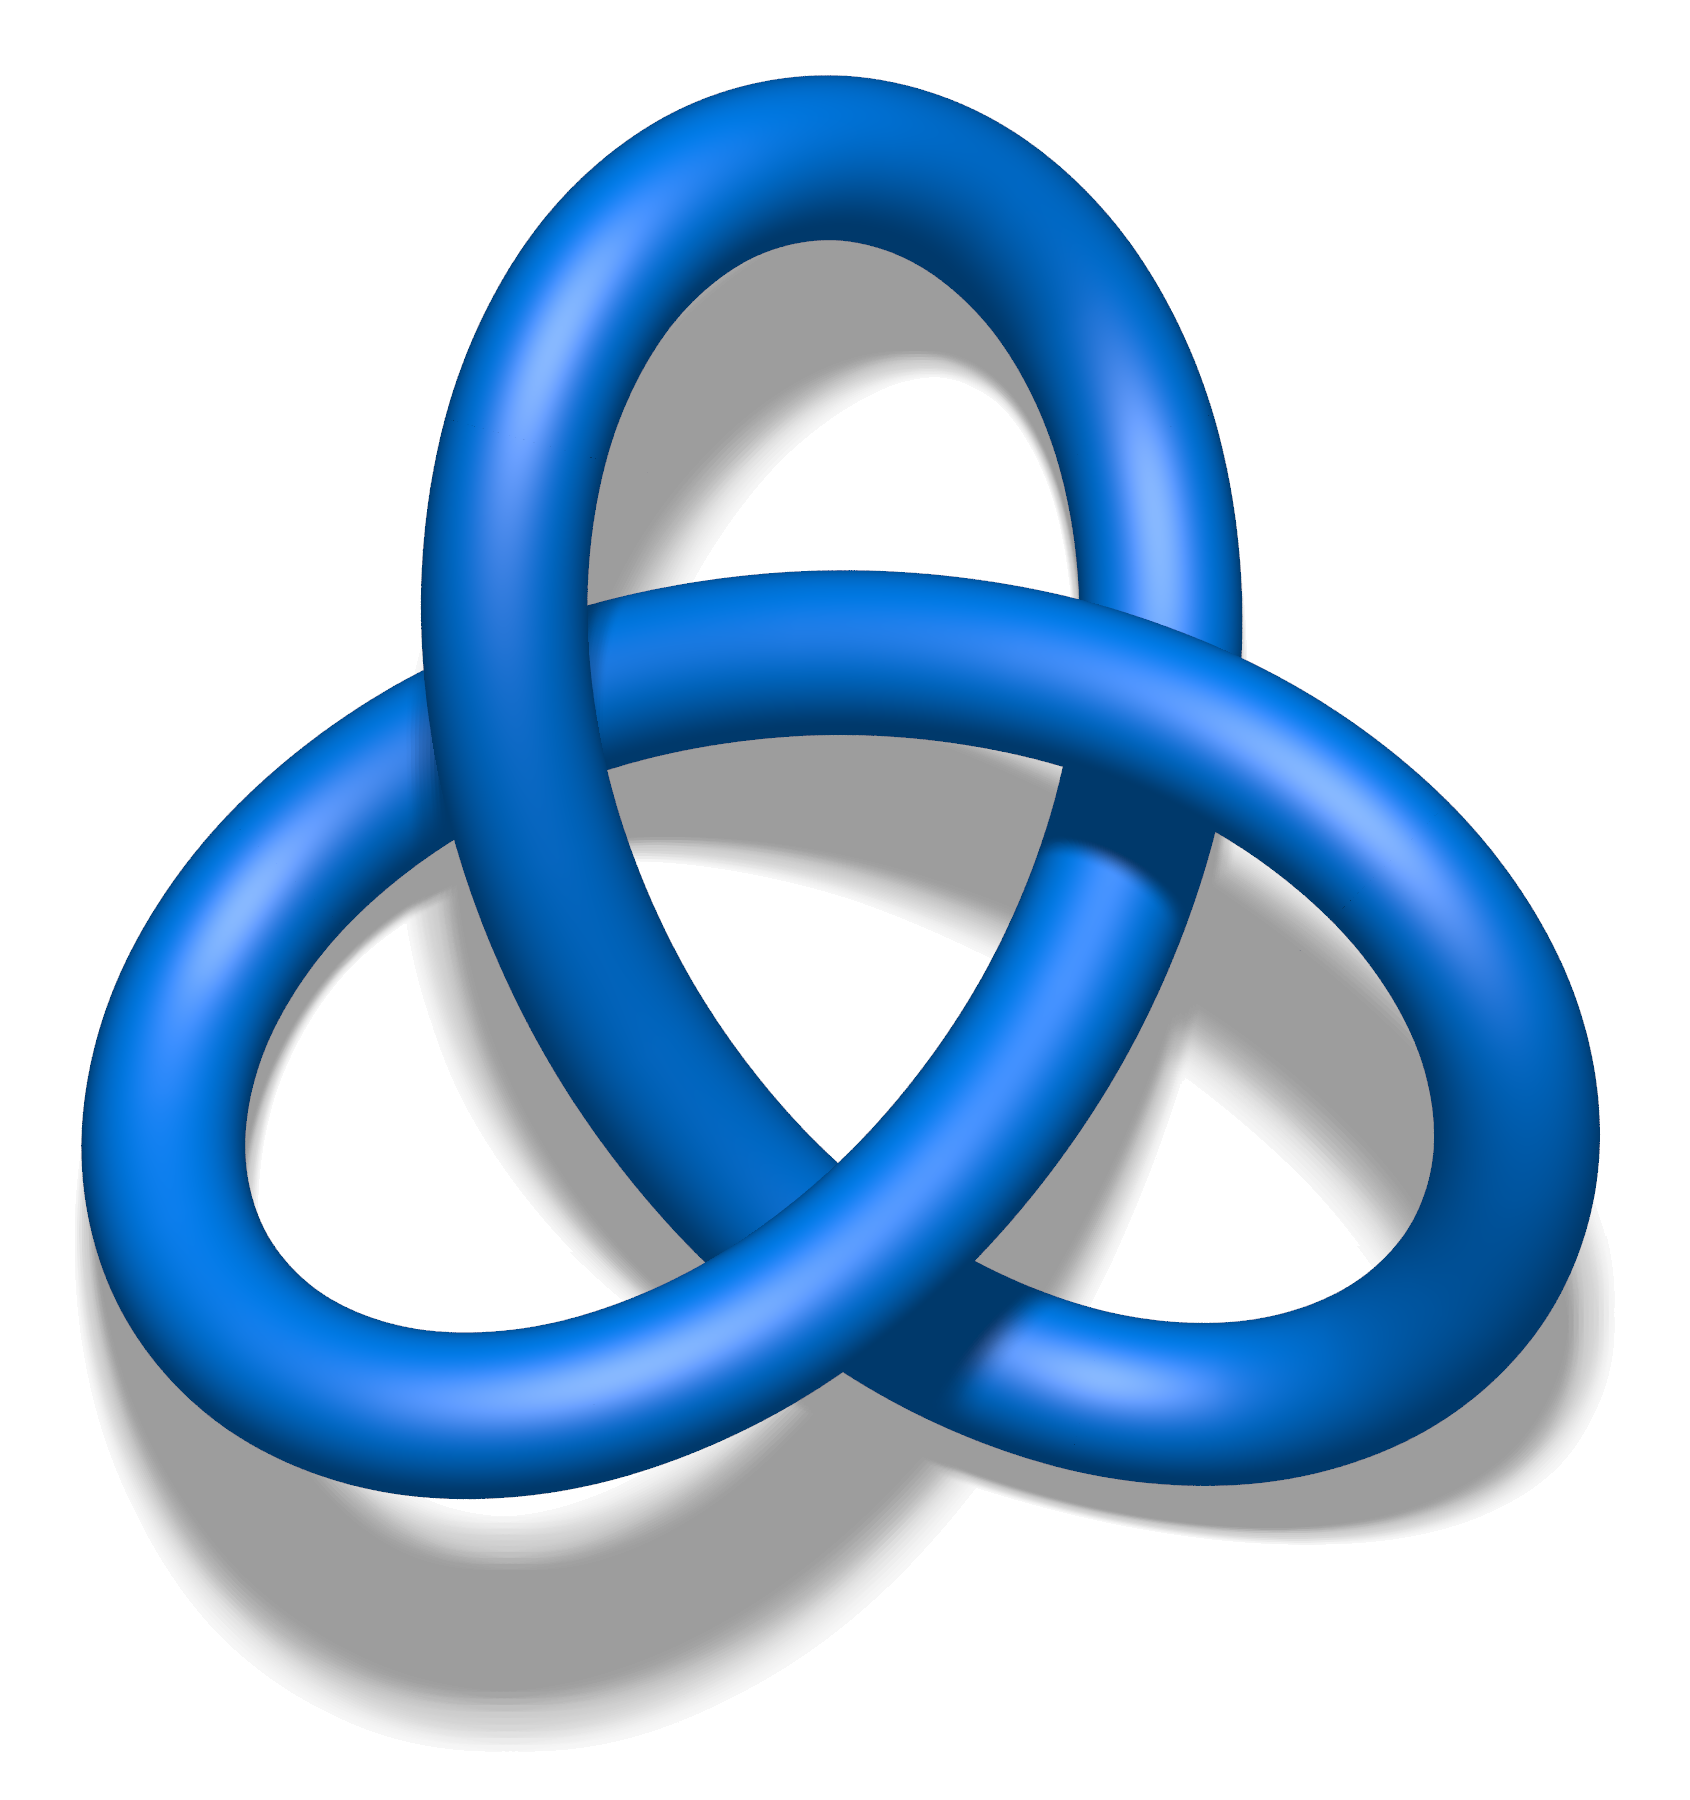
\includegraphics[width=\paperwidth]{Images/trefoil.png}};    

\draw (current page.center) 
	node [fill=white!70, fill opacity=1,text opacity=1,inner sep=1cm]
	{\Huge\centering\bfseries\sffamily\parbox[c][][t]{\paperwidth}{\centering
	 Uma ``rápida'' viagem na teoria dos nós e tranças \\[15pt] % Book title
	{\Large Notas produzidas por Caio Tomás de Paula} \\[20pt] % Subtitle
	{\huge Orientadora: Sheila Campos Chagas}}}; % Author name
\end{tikzpicture}

	\pagestyle{fancy} \addtolength{\headwidth}{\marginparsep}
	\addtolength{\headwidth}{-0.3cm}
	\renewcommand{\headrulewidth}{1pt}
	
	\fancyhf{} \fancyhead[RO,RE]{\small\bfseries\textrm \thepage}
	\fancyhead[LO]{\small\bfseries\textrm \leftmark}
	\fancyhead[LE]{\small\bfseries\textrm \rightmark}
	
	\pagenumbering{roman}
	\tableofcontents
	\newpage
	\pagenumbering{arabic}
	
	\setlength{\baselineskip}{7mm} 
	
	\part{Preliminares}
	
	%----------------------------------------------
	
	\chapter{Grupos de permutação}\label{capitulo grupos de permutacao}
	\begin{lemma}
		\label{lema identidade permutacoes}
		\hspace{12pt} Se $e = \beta_{1}\beta_{2}\cdots\beta_{r}$, com $\beta$ sendo ciclos de tamanho 2, então $r$ é par.
	\end{lemma}
	\begin{proof}
		\vspace{0.3cm}\par Suponha $r>2$. Então, $\beta_{r-1}\beta_{r}$ tem uma das seguintes formas:
		\begin{align}
		e &= (ab)(ab) \\
		(ab)(bc) &= (ac)(ab) \\
		(ac)(cb) &= (bc)(ab) \\
		(ab)(cd) &= (cd)(ab) 
		\end{align}
		Se (1.1) ocorre, então $e = \beta_{1}\beta_{2}\cdots\beta_{r-2}$ e, pelo Segundo Princípio da Indução, $r-2$ é par e, portanto, $r$ é par. Se (1.2), (1.3) ou (1.4) ocorre, podemos substituir o lado direito pelo lado esquerdo em $e$, levando a última ocorrência de $a$ para o penúltimo ciclo da esquerda para a direita. Prosseguindo dessa maneira para reescrever os pares da forma $\beta_{i-1}\beta_{i}$, temos de, em algum momento, obter uma sequência com $r-2$ ciclos de tamanho 2. Porque, do contrário, teríamos
		\begin{equation*}
		e = (a \star)\cdots\gamma_{r}
		\end{equation*}   
		sendo $(a\star)$ a única ocorrência de $a$. Logo, $a$ seria levado em um elemento distinto de $a$ e teríamos um absurdo, pois $e$ fixa todos os  elementos. Portanto, devemos ter uma sequência de $r-2$ ciclos. Pelo Segundo Princípio da Indução Matemática, $r-2$ é par, logo $r$ é par.
	\end{proof}
	\par\vspace{0.3cm} Ao invés de ``ciclos de tamanho $2$'' ou ``$2$-ciclos'', podemos usar o termo \textit{transposições}. De fato, essa nomenclatura é mais intuitiva, pois o que uma permutação de $2$ elementos faz é trocar os dois de lugar, ou seja, transpô-los.
	\par\vspace{0.3cm} Vamos chamar de $A_n$ o conjunto das permutações pares de $n$ elementos, ou seja, as permutações de $n$ elementos que podem ser decompostas em um produto de um número par de transposições. De fato, $A_n$ é subgrupo de $S_n$, como demonstrado abaixo.
	\begin{theorem}
		\label{grupo alternante subgrupo de S_n}
		$A_n \leq S_n$.
	\end{theorem}
	\begin{proof}
	Se $\alpha, \beta \in A_n$, então $\alpha\beta = \sigma_1\sigma_2\cdots\sigma_r\gamma_1\gamma_2\cdots\gamma_s \in A_n$, pois $r+s$ é par já que $r$ e $s$ são pares. \end{proof}
	\begin{theorem}
		\label{ordem do grupo alternante}
		Para todo $n>1, |A_n| = \displaystyle{\frac{n!}{2}}$.\end{theorem}
	\begin{proof}
		Como toda permutação pode ser escrita como produto de ciclos de tamanho 2, sabemos que se $\alpha\in S_n$, $\alpha$ é par ou $\alpha$ é ímpar. 
		\par\vspace{0.3cm} Se $\alpha$ é par, então $(12)\alpha$ é ímpar. Além disso, $(12)\alpha\neq (12)\beta$ para $\alpha\neq\beta$. Logo, a quantidade de permutações pares é maior ou igual à de permutações ímpares, pois multiplicar uma permutação par por $(12)$ gera uma permutação ímpar, mas pode não gerar \textbf{todas} as permutações ímpares.
		\par\vspace{0.3cm} Por outro lado, se $\alpha$ é ímpar, então $(12)\alpha$ é par. Novamente, $(12)\alpha\neq (12)\beta$ para $\alpha\neq\beta$. Logo, a quantidade de permutações ímpares é maior ou igual à de permutações pares, pois multiplicar uma permutação ímpar por $(12)$ gera uma permutação par, mas pode não gerar \textbf{todas} as permutações pares. 
		\par\vspace{0.3cm} Portanto, a quantidade de permutações pares é igual à quantidade de permutações ímpares, logo $|A_n| = \displaystyle{\frac{|S_n|}{2} = \frac{n!}{2} }$. \end{proof} 
	
	%\begin{example}
	%	Mostre que podemos escrever $(16523)$ como combinação de $(13456)$ e $(132)$.
	%\end{example}
	
	%\begin{proof}
	%	Sejam $r = (13456)$ e $s = (132)$. Queremos obter o ciclo $\alpha = (16523) = (13)(12)(15)(16)$. Note que $\alpha$ é par. Com programas de computador, sabemos que $|\langle r,s\rangle| = 360 = |A_6|$, logo $\langle r,s\rangle = A_6$. Como $\alpha\in A_6$, então podemos obter $\alpha$ a partir de $r$ e $s$.
	%\end{proof} 
	\par\vspace{0.3cm} Por exemplo, podemos escrever a permutação $(16523)$ como combinação das permutações $(13456)$ e $(132)$. De fato, façamos $r = (13456)$ e $s = (132)$. Queremos obter o ciclo $\alpha = (16523) = (13)(12)(15)(16)$. Note que $\alpha$ é uma permutação par. Com alguns cálculos (preferencialmente em computadores), podemos obter que $|\langle r,s \rangle| = 360 = |A_6|$, logo $A_6 = \langle r,s \rangle$. Como $\alpha\in A_6$, então é claro que podemos obtê-la a partir de $r$ e $s$.
	
	\chapter{Isomorfismos}\label{capitulo isomorfismos}
	
	\begin{definition}
		\label{def isomorfismo}
		Um \textbf{isomorfismo} $\phi$ de um grupo $G$ em um grupo $\overline{G}$ é uma aplicação bijetora de $G$ em $\overline{G}$ que preserva a operação, isto é, $\phi(ab) = \phi(a)\phi(b),\forall a,b\in G$.
	\end{definition}
	\par\vspace{0.3cm} Na Definição \eqref{def isomorfismo}, no lado esquerdo da igualdade a operação é a de $G$, enquanto que no lado direito a operação é a de $\overline{G}$.
	
	\begin{theorem}[Teorema de Cayley]
		\label{Cayley}
		Todo grupo é isomorfo a um grupo de permutações.
	\end{theorem}
	
	\begin{proof}
		Seja $G$ um grupo. Para qualquer $g\in G$, defina $T_g:G\to G$ por $T_g(x) = gx, \forall x\in G$. Note que $T_g$ é uma permutação no conjunto de elementos de $G$, pois cada elemento $x\in G$ é levado no elemento $gx$, também em $G$. 
		\par\vspace{0.3cm} Agora, seja $\overline{G} = \{ T_g | g\in G \}$. Então, $\overline{G}$ é um grupo sob a composição. Para verificar isso, observe que para quaisquer $g$ e $h$ em $G$, temos $T_gT_h(x) = T_g(T_h(x)) = T_g(hx) = g(hx) = (gh)x = T_{gh}(x)$, logo $T_gT_h = T_{gh}$.
		\par\vspace{0.3cm} Daí, segue que $T_e$ é a identidade, e $(T_g)^{-1} = T_{g^{-1}}$. Como a composição é associativa, $\overline{G}$ é grupo.
		\par\vspace{0.3cm} Agora, podemos definir $\phi: G\to\overline{G}$ dado por $\phi(g) = T_g, \forall g\in G$. Se $T_g = T_h$, então $T_g(e) = T_h(e)$ ou, equivalentemente, $ge = he$. Então, $g = h$ e $\phi$ é injetora. Pela maneira que construímos $\overline{G}$, vemos que $\phi$ é sobrejetora. Por fim, sejam $a,b\in G$ quaisquer. Então
		\begin{align*}
		\phi(ab) = T_{ab} = T_aT_b = \phi(a)\phi(b)
		\end{align*}
	\end{proof}
	\par\vspace{0.3cm} Os isomorfismos têm algumas propriedades, listadas a seguir nos Teoremas \eqref{isomorfismos em elementos} e \eqref{isomorfismos em grupos}.
	
	\begin{theorem}
		\label{isomorfismos em elementos}
		\begin{enumerate}
			\item \vspace{0.3cm} $\phi$ leva a identidade de $G$ na identidade de $\overline{G}$;
			\item $\forall n\in\mathbb{N}, a\in G, \phi (a^n) = [\phi (a)]^n$;
			\item Dados $a,b \in G$ quaisquer, $ab = ba \Leftrightarrow \phi (a)\phi (b) = \phi (b)\phi (a)$;
			\item $G = \langle a \rangle \Leftrightarrow \overline{G} = \langle\phi(a) \rangle$;
			\item $|a| = |\phi(a)|, \forall a\in G$;
			\item Dados $k\in\mathbb{Z}$ e $b\in G$, a equação $x^k = b$ tem a mesma quantidade de soluções em $G$ que a equação $x^k = \phi(b)$ tem em $\overline{G}$;
			\item Se $G$ é finito, $G$ e $\overline{G}$ têm o mesmo número de elementos de cada ordem. 
		\end{enumerate}
	\end{theorem}
	
	\begin{proof}
		\textbf{1.} Sejam $e$, $\overline{e}$ as identidades de $G$ e $\overline{G}$, respectivamente. Logo, temos:
		\begin{equation*}
		e = e\cdot e \Rightarrow \phi (e) = \phi (e)\phi (e)
		\end{equation*} 
		Como $\phi (e)\in \overline{G}$, segue que $\phi(e) = \overline{e}$. 
		\par\vspace{0.4cm}
		\textbf{2.} Se $n=0$, temos $\phi (e) = \overline{e} = (\overline{e})^0$. 
		Para $n>0$, temos $\phi (a^n) = \underbrace{\phi (a)\phi (a)\dots \phi (a)}_{n} = [\phi (a)]^n$.
		Agora, se $n<0$, então $-n>0$ e temos:
		\begin{equation*}
		\phi (e) = \overline{e} = \phi (a^n a^{-n}) = \phi (a^n)[\phi (a)]^{-n} \Rightarrow [\phi (a)]^n = \phi (a^n)
		\end{equation*}
		\par\vspace{0.4cm}
		\textbf{3.} Sejam $a,b \in G$. Temos que:
		\par
		\begin{equation*}
		(\Rightarrow) \hspace{12pt}ab = ba \Rightarrow \phi (ab) = \phi (ba) \Rightarrow \phi (a)\phi (b) = \phi (b)\phi (a)
		\end{equation*}
		\par
		\begin{equation*}
		(\Leftarrow)\hspace{12pt}\phi(a)\phi(b) = \phi(b)\phi(a) \Rightarrow \phi(ab) = \phi(ba) \Rightarrow ab = ba
		\end{equation*}
		em que a volta é devido à injetividade de $\phi$.
		\par\vspace{0.4cm}
		\textbf{4.} Seja $G = \langle a \rangle $. Como $\overline{G}$ é fechado, $\langle \phi(a)\rangle \subseteq \overline{G}$. Como $\phi$ é sobrejetora, então para todo $b\in\overline{G}$, existe $k$ inteiro tal que $b = \phi(a^k) = [\phi(a)]^k \in\langle \phi(a)\rangle $, logo $\overline{G}\subseteq\langle \phi(a)\rangle$ e, portanto, $\overline{G} = \langle \phi(a)\rangle.$
		\par\vspace{0.3cm} Agora, seja $\overline{G} = \langle \phi(a)\rangle$. Como $G$ é fechado, $\langle a\rangle \subseteq G$. Note que $\forall b\in G, \phi(b)\in\langle \phi(a)\rangle$, i.e., existe $k\in\mathbb{Z}$ tal que $\phi(b) = [\phi(a)]^k = \phi(a^k)$. Logo, como $\phi$ é injetora, $b = a^k\in\langle a\rangle $ e $G \subseteq \langle a\rangle$. Portanto, $G = \langle a\rangle$. 
		\par\vspace{0.4cm}
		\textbf{5.} Seja $a\in G$ com $|a| = n$ e $|\phi(a)| = k$. Então:
		\begin{equation*}
		\phi(a^n) = \overline{e} = [\phi(a)]^n.
		\end{equation*}
		logo $k|n$
		.	\par Por outro lado, temos que:
		\begin{equation*}
		[\phi(a)]^k = \overline{e} \Rightarrow a^k = e
		\end{equation*}
		logo $n|k$. Portanto, $n = k$.
		\par\vspace{0.4cm}
		\textbf{6.} Seja $a \in G$ tal que $a^k = b$. Então, $\phi(a^k) = [\phi(a)]^k = \phi(b)$, ou seja, se $a$ é solução de $x^k = b$ em $G$, então $\phi(a)$ é solução de $x^k = b$ em $\overline{G}$. Como $\phi$ é injetora, $\phi(a)\neq\phi(b)$ quando $a\neq b$, ou seja, soluções diferentes da equação em $G$ levam a soluções diferentes da equação em $\overline{G}$. 
		\par\vspace{0.4cm}
		\textbf{7.} Como $|a| = |\phi(a)|$ para todo $a\in G$, então se $G$ tem $k$ elementos de ordem $n_k$, então $\overline{G}$ também terá $k$ elementos de ordem $n_k$ devido à injetividade de $\phi$.	
		
	\end{proof}  
	\par\vspace{0.3cm}
	
	\begin{theorem}
		\label{isomorfismos em grupos}
		\begin{enumerate}
			\item Se $\phi$ é um isomorfismo de $G$ em $\overline{G}$, então $\phi ^{-1}$ é um isomorfismo de $\overline{G}$ em $G$;
			\item $G$ é abeliano se, e só se, $\overline{G}$ é abeliano;
			\item $G$ é cíclico se, e só se, $\overline{G}$ é cíclico;
			\item Se $K$ é um subgrupo de $G$, então $\phi(K) = \{\phi(k)|k\in K\}$ é um subgrupo de $\overline{G}$;
			\item Se $\overline{K}$ é subgrupo de $\overline{G}$, então $\phi^{-1}(\overline{K}) = \{ g\in G|\phi(g)\in\overline{K}\}$ é subgrupo de $G$;
			\item $\phi(Z(G)) = Z(\overline{G})$.
		\end{enumerate}	
	\end{theorem}
	\begin{proof}
		\textbf{1.} Como $\phi$ é bijetiva, $\phi^{-1}$ também é. Logo, basta verificarmos se $\phi^{-1}$ preserva a operação. 
		\par\vspace{0.3cm} Para isso, note que 
		\begin{align*}
		\phi^{-1}(ab) = \phi^{-1}(a)\phi^{-1}(b) \Leftrightarrow ab = \phi(\phi^{-1}(a))\phi(\phi^{-1}(b)) \Leftrightarrow ab = ab.
		\end{align*} 
		Logo, $\phi^{-1}$ de fato preserva a operação.
		\par\vspace{0.4cm}
		\textbf{2.} Pela propriedade 3 do Teorema \eqref{isomorfismos em elementos}, sabemos que $ab = ba$ se, e somente se, $\phi(a)\phi(b) = \phi(b)\phi(a)$, ou seja, os elementos de $G$ comutam se, e só se, os elementos de $\overline{G}$ comutam.
		\par\vspace{0.4cm}
		\textbf{3.} O resultado segue da propriedade 4 do \eqref{isomorfismos em elementos}, que diz que $G = \langle a\rangle \Leftrightarrow \overline{G} = \langle \phi(a)\rangle$.
		\par\vspace{0.4cm}
		\textbf{4.} Sejam $k_1, k_2 \in K$ quaisquer. Temos que:
		\begin{equation*}
		\phi(k_1)\phi(k_2^{-1}) = \phi(k_1k_2^{-1}) \in\phi(K)
		\end{equation*}
		pois $k_1k_2^{-1} \in K$ já que $K$ é subgrupo. 
		\par\vspace{0.4cm}
		\textbf{5.} Se $\overline{K}$ é subgrupo de $\overline{G}$, então para quaisquer $\phi(g_1), \phi(g_2^{-1})\in \overline{K}$, temos:
		\begin{align*}
		\phi^{-1}(\phi(g_1))\phi^{-1}(\phi(g_2^{-1})) = \phi^{-1}(\underbrace{\phi(g_1)\phi(g_2^{-1})}_{\in\overline{K}}) \in \phi^{-1}(\overline{K})
		\end{align*}
		\par\vspace{0.3cm} Portanto, $\phi^{-1}(\overline{K})$ é subgrupo de $G$.
		\par\vspace{0.4cm}
		\textbf{6.} Por definição, sabemos que $Z(G) = \{ z|gz = zg, \forall g\in G \}$. Daí, $\phi(Z(G)) = \{ \underbrace{\phi(z)}_{\in \overline{G}} | \phi(g)\phi(z) = \phi(z)\phi(g), \forall \phi(g)\in\overline{G}\}$, que é, por definição, $Z(\overline{G})$.
		
	\end{proof}
	\par\vspace{0.3cm} Na Definição \eqref{def isomorfismo}, nada nos impede de tomar $G = \overline{G}$. De fato, se o fizermos, obtemos um tipo de isomorfismo especial, chamado automorfismo.
	
	\begin{deff}
		\label{def automorfismo}
		Um isomorfismo de um grupo $G$ em si mesmo é chamado automorfismo. O conjunto de todos os automorfismos de um grupo $G$ é denotado por $\aut(G)$.
	\end{deff}
	\par\vspace{0.3cm} Além disso, podemos ainda definir um tipo especial de automorfismo, chamado automorfismo interno.
	\begin{deff}
		\label{def automorfismo interno}
		O automorfismo de $G$ definido por $\phi_a(x) = axa^{-1}$ para todo $x$ em $G$ é chamado automorfismo interno de $G$ induzido por $a$. O conjunto de todos os automorfismos internos de um grupo $G$ é denotado por $\inn(G)$.
	\end{deff}
	\par\vspace{0.3cm} Um fato interessante de $\aut(G)$ e $\inn(G)$ é o seguinte.
	\begin{theorem}
		$\aut(G)$ e $\inn(G)$ são grupos sob composição.
	\end{theorem}
	\begin{proof}
		\vspace{0.3cm}\par Sejam $\phi_a$ e $\phi_b$ elementos quaisquer de $\inn(G)$. Note que $(\phi_a\circ\phi_b)(x) = \phi_a(\phi_b(x)) = a(bxb^{-1})a^{-1} = abxb^{-1}a^{-1} = (ab)x(ab)^{-1} = \phi_{ab}(x) \in \inn(G)$, logo $\inn(G)$ é fechado para a composição. Além disso, a composição é associativa, $\phi_e(x) = x$ e $(\phi_a\circ\phi_{a^{-1}})(x) = \phi_e(x)$, ou seja, $\inn(G)$ tem identidade e contém os inversos. Logo, $\inn(G)$ é grupo sob composição.
		
		\vspace{0.3cm}\par Agora, sejam $\alpha$ e $\beta$ elementos quaisquer de $\aut(G)$. Note que 
		\begin{equation*}
		\alpha^{-1}(xy) = \alpha^{-1}(x)\alpha^{-1}(y) \Leftrightarrow xy = \alpha(\alpha^{-1}(x)\alpha^{-1}(y)) \Leftrightarrow xy = \alpha(\alpha^{-1}(xy))\ \Leftrightarrow xy = xy
		\end{equation*}
		logo $\alpha^{-1}$ preserva a operação de $G$. Como $\alpha^{-1}$ é bijetiva, então é um isomorfismo, ou seja, temos $\alpha^{-1}\in \aut(G)$. Além disso, como a composição de funções é associativa, $(\alpha\circ\beta)(x) = \alpha(\underbrace{\beta(x)}_{\in G}) \in \aut(G)$ e o isomorfismo $\theta(x) = x$ é a identidade, concluímos que $\aut(G)$ é grupo sob composição.\end{proof}
	\par\vspace{0.3cm} Por exemplo, se tomarmos $(\mathbb{C^{*}}, \cdot)$, o grupo dos complexos não nulos com a multiplicação, e defirnirmos a função $\phi : \mathbb{C^{*}}\to\mathbb{C^{*}}$ tal que $\phi(a+bi) = a-bi$, com $a,b\in\mathbb{R}$, então $\phi$ é automorfismo de $\mathbb{C^{*}}$. 
	\par\vspace{0.3cm} De fato, note que se $\phi(a+bi) = \phi(c+di)$, então:
	\begin{equation*}
	a = bi = c - di \Leftrightarrow \begin{cases}a = b \\ c = d\end{cases}
	\end{equation*}
	\par\vspace{0.3cm} logo $\phi$ é injetora.  Além disso, se $\alpha\in\mathbb{C^{*}}$, então existe $\beta\in\mathbb{C^{*}}$ tal que $\phi(\beta) = \alpha$, a saber, $\beta = \overline{\alpha}$. Logo, $\phi$ é sobrejetora. 
	\par\vspace{0.3cm} Por fim, temos que 
	\begin{align*}
	&\phi[(a + bi)(c + di)] = \phi[(ac - bd) + (ad + bc)i] \\ &= (ac - bd) - (ad + bc)i = (a- bi)(c - di) \\ &= \phi(a + bi)\cdot\phi(c + di)
	\end{align*}.
	\par\vspace{0.3cm} Logo, $\phi$ preserva a operação e, portanto, é automorfismo.
	\par\vspace{0.3cm} Outro exemplo é o conjunto de automorfismos internos de $D_4$, o grupo diedral de ordem $8$. Vamos mostrar que $\inn(D_4) = \displaystyle{ \left\{ \phi_{R_0}, \phi_{R_{90}}, \phi_{H}, \phi_{D} \right\} }$. De fato, para tal basta mostrarmos que $\phi_{R_0}, \phi_{R_{90}}, \phi_{H}, \phi_{D}$ são todos distintos. Para isso, basta notar que
	\begin{align*}
	\phi_{R_{0}}(H) = H &\neq V = \phi_{R_{90}}(H) \\
	\phi_{R_{0}}(R_{90}) = R_{90} &\neq R_{270} = \phi_{H}(R_{90}) \\
	\phi_{R_{0}}(R_{270}) = R_{270} &\neq R_{90} = \phi_{D}(R_{270}) \\
	\phi_{R_{90}}(R_{90}) = R_{90} &\neq R_{270} = \phi_{H}(R_{90}) \\
	\phi_{R_{90}}(R_{90}) = R_{90} &\neq R_{270} = \phi_{D}(R_{90}) \\
	\phi_{H}(V) = V &\neq H = \phi_{D}(V)
	\end{align*}
	\par\vspace{0.3cm} Logo, $\phi_{R_0}, \phi_{R_{90}}, \phi_{H}, \phi_{D}$ são, de fato, todos distintos. 
	\par\vspace{0.3cm} Em geral, dado um grupo $G$ não é simples determinar $\aut(G)$ e $\inn(G)$. Contudo, para alguns grupos conseguimos fazê-lo com relativa facilidade. Um desses grupos é $\mathbb{Z}_n$.
	\begin{theorem}
		\label{automorfismos de Z_n}
		$\aut(\mathbb{Z}_n) \cong U(n)$.
	\end{theorem}
	
	\begin{proof}
		Seja $T: \aut(\mathbb{Z}_n)\to U(n)$ tal que $\alpha\mapsto\alpha(1)$, ou seja, o automorfismo $\alpha$ é levado na imagem de $1$ por $\alpha$. Como $a(k) = k\alpha(1)$, $T$ é injetora, pois se $\alpha(1) = \beta(1)$, então $\alpha(k) = k\alpha(1) = k\beta(1) = \beta(k)$, logo $\alpha = \beta$. 
		\par\vspace{0.3cm} Agora, seja $r\in U(n)$ e tome o automorfismo $\alpha$ de $\mathbb{Z}_n$ dado por $\alpha(s) = sr \pmod n$. Como $T(\alpha) = \alpha(1) = r\pmod n = r$, $T$ é sobrejetora.
		\par\vspace{0.3cm} Por fim, sejam $\alpha$ e $\beta$ elementos quaisquer de $\aut(\mathbb{Z}_n)$. Então, temos:
		\begin{align*}
		T(\alpha\circ\beta) = (\alpha\circ\beta)(1) = \alpha(\beta(1)) = \alpha(\underbrace{1 + 1 + \cdots + 1}_{\beta(1)}) = \underbrace{\alpha(1) + \alpha(1) + \cdots + \alpha(1)}_{\beta(1)} = \alpha(1)\cdot\beta(1).
		\end{align*}
		\par\vspace{0.3cm} Logo, $T$ preserva a operação e, portanto, é isomorfismo.
	\end{proof}
	\par\vspace{0.3cm} Outro exemplo é $\aut(\mathbb{Z})$.	Pela propriedade 4 do Teorema \eqref{isomorfismos em elementos}, um isomorfismo deve levar gerador em gerador. Como $\mathbb{Z}$ possui apenas dois geradores, $1$ e $-1$, há apenas dois automorfismos em $\aut(\mathbb{Z})$: o automorfismo identidade, que leva $1$ em $1$ e $-1$ em $-1$; e o automorfismo que leva $1$ em $-1$ e $-1$ em $1$.
	
	
	\begin{remark}
		Pelo Teorema \eqref{automorfismos de Z_n}, $|\aut(\mathbb{Z}_n)| = |U(n)| = \phi(n)$ (sendo $\phi(n)$ a função totiente de Euler). Por outro lado, vemos, a partir do que fizemos acima, que $|\aut(\mathbb{Z})| = 2$. Logo, em geral, $|\aut(\mathbb{Z}_n)| > |\aut(\mathbb{Z})|$, pois em geral $\phi(n) > 2$.
	\end{remark}
	
	\chapter{Classes laterais} \label{capitulo classes laterais}
	\hspace{12pt} Um conceito importante no estudo de grupos é o de \textbf{classes laterais}.
	\begin{deff}
		\label{def classes laterais}
		Sejam $G$ um grupo e $H$ um subconjunto não vazio de $G$. Para qualquer $a\in G$,	o conjunto $\{ah | h \in H \}$ é denotado por $aH$. Analogamente, $Ha = \{ha | h \in H\}$
		e $aHa^{-1} = \{aha^{-1} | h \in H\}$. Quando $H$ é subgrupo de $G$, o conjunto $aH$ é dito classe lateral à esquerda de $H$ em $G$ contendo $a$, enquanto que $Ha$ é dito classe lateral à direita de $H$ em $G$ contendo $a$. Nesse caso, o elemento $a$ é dito o representante da classe lateral $aH$ (ou $Ha$). Usamos $|aH|$ para denotar o número de elementos no conjunto $aH$, e $|Ha|$ para denotar o número de elementos em $Ha$.
	\end{deff}
	\par\vspace{0.3cm} Assim como os isomorfismos, as classes laterais têm propriedades, listadas a seguir no Lema \eqref{propriedades}.
	\begin{lemma}
		\label{propriedades}
		\begin{enumerate}
			\item $a\in aH$ (a classe lateral à esquerda de $H$ contendo $a$ contém $a$); 
			\item $aH = H \Leftrightarrow a\in H$ (a classe lateral absorve um elemento se, e só se, esse elemento está em $H$);
			\item $(ab)H = a(bH)$ e $H(ab) = (Ha)b$;
			\item $aH = bH \Leftrightarrow a\in bH$ (uma classe lateral é unicamente determinada por um de seus elementos);
			\item $aH = bH$ ou $aH \cap bH = \emptyset$ (duas classes laterais ou são iguais ou disjuntas);
			\item $aH = bH \Leftrightarrow a^{-1}b\in H$ (uma questão de classe lateral se torna uma questão sobre $H$);
			\item $|aH| = |bH|$ (todas as classes laterais têm mesmo tamanho);
			\item $aH = Ha \Leftrightarrow H = aHa^{-1}$;
			\item $aH$ é subgrupo de $G$ se, e só se, $a\in H$ ($H$ é a única classe lateral que é subgrupo de $G$).
		\end{enumerate}	
	\end{lemma}
	\begin{proof}
		\textbf{1.} Como $e\in H$, então $a = ae \in H$.
		\par\vspace{0.4cm}
		\textbf{2.} Se $aH = H$, então $a\in aH = H$. Por outro lado, se $a\in H$, é claro que $aH\subseteq H$. Além disso, se $h\in H$, então $a^{-1}h\in H$, pois $a^{-1}\in H$ já que $H$ é subgrupo. Logo, $h = (aa^{-1})h = a(a^{-1}h)\in aH$. Portanto, $H\subseteq aH$ e $H = aH$. 
		\par\vspace{0.4cm}
		\textbf{3.} Como $(ab)h = a(bh)$ e $h(ab) = (ha)b$, o resultado segue.
		\par\vspace{0.4cm}
		\textbf{4.} Se $aH = bH$, então $a = ae\in aH = bH$. Por outro lado, se $a\in bH$, então $a = bh$, para algum $h\in H$, logo, $aH = (bh)H = b(hH) \overset{\textbf{2}}{=} bH$.
		\par\vspace{0.4cm}
		\textbf{5.} Note que se $c\in aH\cap bH$, então $c\in aH$ e $c\in bH$, i.e., $cH = aH = bH$. Logo, se $aH\cap bH\neq\emptyset$, $aH = bH$.
		\par\vspace{0.4cm}
		\textbf{6.} Temos que
		\begin{equation*}
		aH = bH \Leftrightarrow H = (a^{-1}b)H \overset{\textbf{2}}{\Leftrightarrow} a^{-1}b \in H
		\end{equation*}
		\par\vspace{0.4cm}
		\textbf{7.} Se $aH = bH$, terminamos. Então, seja $f: aH\to bH$ tal que $f(x) = b^{-1}ax$. Tomando $x_1$ e $x_2$ em $aH$, temos que $f(x_1) = f(x_2)$ implica $x_1=x_2$, logo $f$ é injetiva. Além disso, tomando $a^{-1}by$ em $aH$, sendo $y\in bH$, temos $f(a^{-1}by) = y$, logo $f$ é sobrejetora. Consequentemente, definimos uma bijeção de $aH$ em $bH$ e, portanto, $|aH| = |bH|$.
		\par\vspace{0.4cm}
		\textbf{8.} Note que $aH = Ha \Leftrightarrow (aH)a^{-1} = H(aa^{-1}) = H$, i.e., se, e só se, $aHa^{-1} = H$.
		\par\vspace{0.4cm}
		\textbf{9.} Se $aH$ é subgrupo de $G$, então $e\in aH$. Então, $aH\cap eH \neq \emptyset$, logo $aH = eH = H$ e, por isso, $a\in H$. Por outro lado, se $a\in H, aH = H$, que é subgrupo de $G$.	
		
	\end{proof}
	\par\vspace{0.3cm} Com a Definição \eqref{def classes laterais} e o Lema \eqref{propriedades}, podemos enunciar o Teorema \eqref{lagrange}.
	\begin{theorem}
		\label{lagrange}
		Se $|G|<\infty$ e $H$ é subgrupo de $G$, então a ordem de $H$ divide a ordem de $G$. Ademais, a quantidade de classes laterais à esquerda (direita) de $H$ em $G$ é $|G|/|H|$, ou seja, a ordem de um subgrupo divide a ordem do grupo. 
	\end{theorem}
	
	\begin{proof}
		Sejam $a_1H, a_2H, \dots , a_rH$ as classes laterais distintas à esquerda de $H$ em $G$. Então, temos $aH = a_iH$ para todo $a$ em $G$ e algum $i = 1,2,\dots,r$. Pela propriedade \textbf{1} do Lema \eqref{propriedades}, $a\in aH$. Logo, temos $aH = H = a_iH$ e, daí:
		\begin{align*}
		G = \bigcup_{1\leq i\leq r}^{}a_iH \Rightarrow |G| = \sum_{1\leq i\leq r}^{}|a_iH| = \sum_{1\leq i\leq r}^{}|H| = r|H|
		\end{align*} 
		\begin{equation*}
		\therefore |G|/|H| = r
		\end{equation*}
		
	\end{proof}
	\par\vspace{0.3cm} Alguns resultados seguem como consequência imediata do Teorema \eqref{lagrange}.
	
	\begin{corollary}
		\label{c2}
		Em um grupo finito, a ordem de cada elemento divide a ordem do grupo.
	\end{corollary}
	
	\begin{proof}
		Como $|a| = |\langle a\rangle|$ e $\langle a \rangle$ é um subgrupo de $G$, então $|a|$ divide $|G|$. 
	\end{proof}
	
	\begin{corollary}
		\label{c3}
		Um grupo de ordem prima é cíclico.
	\end{corollary}
	
	\begin{proof}
		Se $|G| = p$, $p$ primo, e $a\in G$, $a\neq e$, então $|a| = |\langle a\rangle | \neq 1$ divide $|G|$, logo $|a| = p = |G|$. Portanto, $G = \langle a\rangle$. 
	\end{proof}
	
	\begin{corollary}
		\label{c4}
		Seja $G$ um grupo finito, $a\in G$. Então, $a^{|G|} = e.$
	\end{corollary}
	
	\begin{proof}
		Pelo Corolário \eqref{c2}, $|G| = |a| k, k\in\mathbb{Z}_{+}^{*}$. Logo, $a^{|G|} = a^{|a|k} = e^k = e$. 
	\end{proof}
	
	\begin{corollary}[Pequeno Teorema de Fermat]
		\label{c5}
		Para todo $a$ inteiro e para todo primo $p$, $a^p \pmod p = a\pmod p$.
	\end{corollary}
	
	\begin{proof}
		Pelo algoritmo da divisão, podemos escrever $a = pm + r, 0\leq r < p$. Daí, $a\pmod p = r$ e só precisamos mostrar que $r^p\pmod p = r$.
		\par\vspace{0.3cm} Se $r = 0$, então $p|a$ e é claro que $r^p\pmod p = r\pmod p$.
		\par\vspace{0.3cm} Suponha $r>0$. Então, $r\in U(p) = \{1, 2, \dots, p-1\}$, sendo a operação de $U(p)$ a multilicação módulo $p$. Note que $|U(p)| = p-1$. Daí, pelo Corolário \eqref{c4}, temos que $r^{p-1}\pmod p = 1$ e, consequentemente, $r^p\pmod p = r$. 
	\end{proof}
	
	\begin{theorem}
		\label{ordem de HK}
		Para dois subgrupos finitos $H$ e $K$ de um grupo $G$, seja $HK = \left\{ hk| h\in H, k\in K \right\}$. Então, $|HK| = |H||K|/|H\cap K|$.
	\end{theorem}
	
	\begin{proof}
		Apesar do conjunto $HK$ ter $|H||K|$ produtos, nem todos eles são, necessariamente, distintos, isto é, podemos ter $hk = h'k'$ com $h\neq h'$ e $k\neq k'$. Para determinar $|HK|$, devemos descobrir quantas vezes isso ocorre. 
		\par\vspace{0.3cm} Para todo $t$ em $H\cap K$, podemos escrever $hk = (ht)(t^{-1}k)$, então cada elemento de $HK$ pode ser representado por pelo menos $|H\cap K|$ produtos. Mas note que $hk = h'k'$ implica $t = h^{-1}h' = kk'^{-1}\in H\cap K$, logo $h' = ht$ e $k' = t^{-1}k$. Consequentemente, cada elemento em $HK$ pode ser representado por exatamente $|H\cap K|$ produtos. Daí, $|HK| = |H||K|/|H\cap K|$.
	\end{proof}
	\par\vspace{0.3cm} Um exemplo interessante de isomorfismo é o fato de que $S_3\cong GL(2,\mathbb{Z}_2)$. De fato, seja $\phi:GL(2,\mathbb{Z}_2)\to S_3$, e sejam ainda
	\begin{align*}
	v_1 = \begin{bmatrix}
	1 \\
	0
	\end{bmatrix}, 
	v_2 =  \begin{bmatrix}
	0 \\ 
	1
	\end{bmatrix}, 
	v_3 = \begin{bmatrix}
	1 \\ 
	1
	\end{bmatrix}
	\end{align*}
	Todo elemento de $GL(2,\mathbb{Z}_2)$ permuta $v_1, v_2$ e $v_3$.
	\par\vspace{0.3cm} Por exemplo, $\begin{bmatrix}
	1 & 1 \\ 
	0 & 1
	\end{bmatrix}$
	manda $v_1$ em $v_1$, $v_2$ em $v_3$ e $v_3$ em $v_2$, ou seja, nos dá a permutação $(v_2v_3)$.
	\par\vspace{0.3cm} Além disso, note que matrizes diferentes em $GL(2, \mathbb{Z}_2)$ nos dão permutações diferentes de $\{v_1, v_2,v_3\}$, logo $\phi$ é injetiva.
	\par\vspace{0.3cm} Por fim, como $|GL(2, \mathbb{Z}_2)| = 6 = |S_3|$, $\phi$ é sobrejetiva e, portanto, é bijetiva. Logo, é isomorfismo. 
	\par\vspace{0.3cm} Outra demonstração possível é notar que para $S_3$ temos a tabela de multiplicação:
	\begin{table}[H]
		\centering
		\noindent\begin{tabular}{c|cccccc}
			& 1 & (12) & (13) & (23) & (123) & (132) \\
			\hline
			1 & 1 & (12) & (13) & (23) & (123) & (132) \\
			(12) & (12) & 1 & (132) & (123) & (23) & (13) \\
			(13) & (13) & (123) & 1 & (132) & (12) & (23) \\
			(23) & (23) & (132) & (123) & 1 & (13) & (12) \\
			(123) & (123) & (13) & (23) & (12) & (132) & 1 \\
			(132) & (132) & (23) & (12) & (13) & 1 & (123) \\
		\end{tabular}
	\end{table}
	\par \vspace{0.3cm} Fazendo 
	\begin{align*}
	1 = \begin{bmatrix}
	1 & 0 \\
	0 & 1
	\end{bmatrix}, 
	i = \begin{bmatrix}
	0 & 1 \\
	1 & 0
	\end{bmatrix}, 
	j = \begin{bmatrix}
	1 & 1 \\
	0 & 1
	\end{bmatrix}, 
	k = \begin{bmatrix}
	1 & 0 \\
	1 & 1
	\end{bmatrix},
	a = \begin{bmatrix}
	1 & 1 \\
	1 & 0
	\end{bmatrix}, 
	b = \begin{bmatrix}
	0 & 1 \\
	1 & 1
	\end{bmatrix}
	\end{align*} 
	obtemos a seguinte tabela de multiplicação para $GL(2, \mathbb{Z}_2)$:
	\begin{table}[H]
		\centering
		\noindent\begin{tabular}{c|cccccc}
			& 1 & $i$ & $j$ & $k$ & $a$ & $b$ \\
			\hline
			1 & 1 & $i$ & $j$ & $k$ & $a$ & $b$ \\
			$i$ & $i$ & 1 & $b$ & $a$ & $k$ & $j$ \\
			$j$ & $j$ & $a$ & 1 & $b$ & $i$ & $k$ \\
			$k$ & $k$ & $b$ & $a$ & 1 & $j$ & $i$ \\
			$a$ & $a$ & $j$ & $k$ & $i$ & $b$ & 1 \\
			$b$ & $b$ & $k$ & $i$ & $j$ & 1 & $a$ \\
		\end{tabular}
	\end{table}
	\par\vspace{0.3cm} Daí, podemos ver que os dois grupos são isomorfos via $\phi:GL(2, \mathbb{Z}_2)\to S_3$ com 
	\begin{equation*}
	1\mapsto 1, i\mapsto(12), j\mapsto(13), k\mapsto(23), a\mapsto(123), b\mapsto(132).
	\end{equation*}
	\par\vspace{0.3cm}
	
	\begin{deff}
		\label{def estabilizador}
		Seja $G$ um grupo de permutações de um conjunto $S$. Para cada $i\in S$, seja $\stab_G(i) = \{ \phi\in G | \phi(i) = i\}$. Chamamos $\stab_G(i)$ de estabilizador de $i$ em $G$. Usamos $|\stab_G(i)|$ para denotar o número de elementos em $\stab_G(i)$.
	\end{deff}
	
	\begin{deff}
		\label{def orbita}
		Seja $G$ um grupo de permutações de um conjunto $S$. Para cada $s\in S$, seja $\orb_G(s) = \{ \phi(s) | \phi\in G \}$. O conjunto $\orb_G(s)$ é um subconjunto de $S$ e é chamado de órbita de $s$ sob $G$. Usamos $|\orb_G(s)|$ para denotar o número de elementos em $\orb_G(s)$.
	\end{deff}
	
	\begin{theorem}
		\label{orb-stab}
		Seja $G$ um grupo finito de permutações de um conjunto $S$. Então, para todo $i$ em $G$, $|G| = |\orb_G(s)|\cdot|\stab_G(i)|$.
	\end{theorem}
	
	\begin{proof}
		Pelo Teorema \eqref{lagrange}, $|G|/|\stab_G(i)|$ é o número de classes laterais distintas à esquerda de $\stab_G(i)$ em $G$. Logo, para provar o teorema, basta estabelecer um correspondência biunívoca entre as classes laterais à esquerda de $\stab_G(i)$ e os elementos de $\orb_G(s)$. 
		\par\vspace{0.3cm} Para isso, definimos a correspondência $T$ que mapeia a classe lateral $\phi\stab_G(i)$ para $\phi(i)$. 
		\par\vspace{0.3cm} Note que $T$ está bem definida, pois se $\alpha\stab_G(i) = \beta\stab_G(i)$, então, pela propriedade 6 do Lema \eqref{propriedades}, $\alpha^{-1}\beta\in\stab_G(i)$, ou seja, $(\alpha^{-1}\circ\beta)(i) = i$ e, portanto, $\alpha(i) = \beta(i)$.
		\par\vspace{0.3cm} Por outro lado, se $\alpha(i) = \beta(i)$, então $(\alpha^{-1}\circ\beta)(i) = i$. Logo, $\alpha^{-1}\beta\in\stab_G(i)$ e, pela propriedade 6 do Lema \eqref{propriedades}, $\alpha\stab_G(i) = \beta\stab_G(i)$. Logo, $T$ é injetiva. 
		\par\vspace{0.3cm} Por fim, seja $j\in\orb_G(s)$. Então $\alpha(i) = j$ para algum $\alpha \in G$ e é claro que $T(\alpha\stab_G(i)) = \alpha(i) = j$, logo $T$ é sobrejetiva e, portanto, é bijetiva.
		\par\vspace{0.3cm} Mostramos então que $|G|/|\stab_G(i)| = |\orb_G(i)|$, ou seja, $|G| = |\orb_G(i)|\cdot|\stab_G(i)|$. 
		
	\end{proof}
	
	\begin{theorem}
		\label{part}
		O conjunto das órbitas dos elementos de $S$ sob um grupo $G$ particionam $S$.
	\end{theorem}
	
	\begin{proof}
		Sejam $a,b\in S$ quaisquer. É claro que $a\in\orb_G(a)$ e $b\in\orb_G(b)$. 
		\par\vspace{0.3cm} Agora, seja $c\in\orb_G(a)\cap\orb_G(b)$. Então, $c = \alpha(a) = \beta(b)$ para algum $\alpha$ e algum $\beta$.
		\par\vspace{0.3cm} Por um lado, temos que $b = (\beta^{-1}\circ\alpha)(a)$. Logo, se $x\in\orb_G(b)$, então $x = \gamma(b) = (\gamma\circ\beta^{-1}\circ\alpha)(a)\in\orb_G(a)$, para algum $\gamma$, ou seja, $\orb_G(b)\subseteq\orb_G(a)$.
		\par\vspace{0.3cm} Por outro lado, temos que $a = (\alpha^{-1}\circ\beta)(b)$. Daí, se $y\in\orb_G(a)$, então $y = \sigma(a) = (\sigma\circ\alpha^{-1}\circ\beta)(b)\in\orb_G(b)$, para algum $\sigma$, ou seja, $\orb_G(b)\supseteq\orb_G(a)$. 
		\par\vspace{0.3cm} Logo, as órbitas de elementos distintos ou são iguais ou são disjuntas. Por isso, as órbitas particionam $S$, mas não necessariamente particionam igualmente.  
		
	\end{proof}
	
	
	
	\begin{theorem}
		\label{rotacoes iso a S_4}
		O grupo de rotações de um cubo é isomorfo a $S_4$.
	\end{theorem}
	
	\begin{proof}
		Como o grupo de rotações de um cubo tem a mesma ordem de $S_4$, basta mostrar que o grupo de rotações é isomorfo a um subgrupo de $S_4$ (pela propriedade 5 do Teorema \eqref{isomorfismos em grupos}). 
		\par\vspace{0.3cm} Para isso, note que um cubo possui 4 diagonais e o grupo de rotações no cubo induz um grupo de permutações nas diagonais. Contudo, rotações diferentes não provocam, necessariamente, permutações diferentes. Para ver que esse de fato é o caso, vamos mostrar que todas as 24 permutações são obtidas a partir das rotações.
		\par\vspace{0.3cm} Numerando as diagonais consecutivas com 1, 2, 3 e 4, podemos ver que existe uma rotação de 90 graus que nos dá a permutação $\alpha = (1234)$; outra rotação de 90 graus em torno de um eixo perpendicular ao nosso primeiro eixo nos dá a permutação $\beta = (1423)$.
		\par\vspace{0.3cm} Logo, o grupo de permutações induzido pelas rotações contém o subgrupo \\$\{e, \alpha, \alpha^2, \alpha^3, \beta^2, \beta^2\alpha, \beta^2\alpha^2, \beta^2\alpha^3\}$ de 8 elementos e também contém $\alpha\beta$, que tem ordem 3. 
		\par\vspace{0.3cm} Portanto, o grupo de permutações induzido pelas rotações tem ordem 24 (já que sua ordem deve ser divisível por 8 e por 3) sendo, por isso, isomorfo a $S_4$, uma vez que conseguimos obter todas as permutações das diagonais a partir das rotações $\alpha$ e $\beta$ e suas combinações. 
		
	\end{proof}
	
	
	\chapter{Produto direto externo de grupos}\label{capitulo prod dir ext}
	\hspace{12pt} Vamos definir o produto direto externo de grupos, uma maneira de obter novos grupos a partir de grupos já conhecidos.
	\begin{deff}
		\label{def prod direto externo}
		Seja $G_1, G_2, \dots, G_n$ uma coleção finita de grupos. O produto direto externo de $G_1, G_2, \dots, G_n$, denotado por $\displaystyle{G_1\oplus G_2\oplus\cdots\oplus G_n}$, é o conjunto de todas as $n$-tuplas para as quais o $i$-ésimo componente é um elemento de $G_i$ e a operação é efetuada componente a componente.
	\end{deff}
	
	\begin{theorem}
		Seja $\displaystyle{H = \bigoplus_{i=1}^{n}G_i}$, com $G_i$ grupos. Então, $H$ é também um grupo.
	\end{theorem}
	
	\begin{proof}
		Sejam $a_i, b_i\in G_i$. Da Definição \eqref{def prod direto externo}, sabemos que:
		\begin{align*}
		(a_1, a_2, \dots, a_n)(b_1, b_2, \dots, b_n) = (a_1b_1, a_2b_2, \dots, a_nb_n)\in H \text{ pois cada um dos } G_i \text{ é grupo.}
		\end{align*}
		\par Portanto $H$ é fechado. Além disso, temos que:
		\begin{align*}
		(a_1, a_2, \dots, a_n)[(b_1, b_2, \dots, b_n)(c_1, c_2, \dots, c_n)] &= (a_1, a_2, \dots, a_n)(b_1c_1, b_2c_2, \dots, b_nc_n) \\ &= ((a_1b_1)c_1, (a_2b_2)c_2, \dots, (a_nb_n)c_n) \\ &= (a_1b_1, a_2b_2, \dots, a_nb_n)(c_1, c_2, \dots, c_n) \\ &= [(a_1, a_2, \dots, a_n)(b_1, b_2, \dots, b_n)](c_1, c_2, \dots, c_n)
		\end{align*}
		logo a associatividade se mantém em $H$.
		\par\vspace{0.3cm} Podemos ver que a identidade de $H$ é $(e_1, e_2, \dots, e_n)$, sendo $e_i$ a identidade de $G_i$.
		\par\vspace{0.3cm} Por fim, basta notar que o inverso de todo elemento $(a_1, a_2, \dots, a_n)$ em $H$ é $(a_1^{-1}, a_2^{-1}, \dots, a_n^{-1})$.
		
	\end{proof}
	
	\begin{remark}
		Segue da Definição \eqref{def prod direto externo} que $(g_1, g_2, \dots, g_n)^k = (g_1^k, g_2^k, \dots, g_n^k)$, ou seja, a potência é "distribuída" nas entradas.
	\end{remark}
	
	\begin{theorem}
		Todo grupo de ordem 4 é isomorfo a $\mathbb{Z}_4$ ou $\mathbb{Z}_2\oplus\mathbb{Z}_2$.
	\end{theorem}
	
	\begin{proof}
		Seja $G = \{e, a, b, ab\}$. Se $G$ não é cíclico, então $|a| = |b| = |ab| = 2$, pelo Teorema \eqref{lagrange}. Logo, podemos definir o mapeamento $e\to (0,0)$, $a\to (1,0), b\to (0,1)$, $ab\to (1,1)$, que é um isomorfismo de $G$ em $\mathbb{Z}_2\oplus\mathbb{Z}_2$.
		\par\vspace{0.3cm} Se $G$ é cíclico, então é isomorfo a $\mathbb{Z}_4$, pois todo grupo cíclico de ordem $n$ é isomorfo a $\mathbb{Z}_n$. 
		
	\end{proof}
	
	
	\begin{theorem}
		\label{ordem}
		Seja $\displaystyle{\bigoplus_{i \leq n}}G_i = \{(g_1, g_2, \dots , g_n)| g_i\in G_i \}$. Então, 
		$|(g_1, g_2, \dots , g_n)| = \mmc(|g_1|, |g_2|, \dots , |g_n|)$.
	\end{theorem}
	
	\begin{proof}
		Seja $s = \mmc(|g_1|, |g_2|, \dots , |g_n|)$ e $t = |(g_1, g_2, \dots , g_n)|$. 
		\par\vspace{0.3cm} Por um lado, temos que:
		\begin{align*}
		(g_1, g_2, \dots , g_n)^s = (g_1^s, g_2^s, \dots , g_n^s) = (e_1, e_2, \dots , e_n)
		\end{align*}
		pois $s$ é múltiplo de cada $|g_i|$. Logo, $t\leq s$.
		\par\vspace{0.3cm} Por outro lado, temos que:
		\begin{align*}
		(g_1^t, g_2^t, \dots , g_n^t) = (g_1, g_2, \dots , g_n)^t = (e_1, e_2, \dots , e_n)
		\end{align*}
		logo $t$ é um múltiplo comum de $|g_1|, |g_2|, \dots , |g_n|$. Portanto, $s\leq t$ e concluímos que $s = t$, pelo Princípio da Tricotomia. 
		
	\end{proof}
	
	
	\begin{theorem}
		\label{crit}
		Sejam $G$ e $H$ grupos cíclicos finitos. Então, $G\oplus H$ é cíclico se, e só se, $\mdc(|G|, |H|) = 1$, isto é, $|G|$ e $|H|$ são primos entre si.
	\end{theorem}
	
	\begin{proof}
		Sejam $|G| = m$ e $|H| = n$. Daí, $|G\oplus H| = mn$ (pelo Princípio Fundamental da Contagem). Suponha que $G\oplus H$ é cíclico e que $\langle (g, h) \rangle = G\oplus H$. Suponha que $\mdc(m,n) = d$. Como $(g, h)^{mn/d} = ((g^m)^{n/d} , (h^n)^{m/d}) = (e,e)$, temos que $mn = |(g, h)| \leq mn/d$ e, portanto, $d = 1$.
		
		\par\vspace{0.3cm} Agora, suponha que $\mdc(m, n) = 1$ e $G = \langle g  \rangle $ e $H = \langle h \rangle$. Então, $|(g,h)| = \mmc(|g|, |h|) = \mmc(m, n) \overset{\star}{=} mn = |G\oplus H|$, em que em $\star$ usamos o fato de que $\mmc(a,b)\mdc(a,b) = ab$ para quaisquer $a,b\in\mathbb{Z}$.
		Logo, $G\oplus H = \langle (g, h) \rangle$. 
	\end{proof}
	
	\begin{corollary}
		\label{C1}
		Um produto externo direto $G_1\oplus G_2\oplus\cdots\oplus G_n$ de um número finito de grupos cíclicos finitos é cíclico se, e só se, $|G_i|$ e $|G_j|$ são relativamente primos quando $i\neq j$.
	\end{corollary}
	
	\begin{proof}
		Para $n = 2$ temos o Teorema \eqref{crit}. Suponha que o corolário vale para $n = k>2$. Então, para $n = k+1$, temos $\underbrace{G_1\oplus G_2\oplus\cdots\oplus G_k }_{G}\oplus\underbrace{ G_{k+1}}_{H}$. 
		\par\vspace{0.3cm} Sejam $|G_i| = n_i$ para $i = 1, 2, \dots , k + 1$, $\displaystyle{G = \bigoplus_{i=1}^{k}G_i}$ de modo que $\displaystyle{|G| = \prod_{i =1}^{k}n_i}$ e $H = G_{k+1}$. Daí, $\displaystyle{|G\oplus H| = \prod_{i = 1}^{k+1}n_i}$. 
		\par\vspace{0.3cm} Suponha que $G\oplus H = \langle (g_1, g_2, \dots , g_k, h) \rangle$ e que $\displaystyle{\mdc(|G|, |H|)= \mdc\Bigg(\prod_{i = 1}^{k}n_i, n_{k+1}\Bigg) = d}$. Daí, temos:
		\begin{align*}
		(g_1, g_2, \dots, g_k, h)^{\displaystyle{\frac{1}{d}\prod_{i=1}^{k+1}n_i}} = \Bigg((g_1^{n_1})^{\displaystyle{\frac{1}{d}\prod_{i=2}^{k+1}n_i}}  ,\dots, (h^{n_{k+1}})^{\displaystyle{\frac{1}{d}\prod_{i = 1}^{k}n_i}} \Bigg) = (e, e, \dots, e)
		\end{align*}
		Logo, $\displaystyle{ \prod_{i=1}^{k+1}n_i = |(g_1, g_2,\dots, g_k, h)| \leq \frac{1}{d}\prod_{i=1}^{k+1}n_i }$, ou seja, $d = 1$.
		\par\vspace{0.3cm} Como nenhum dos $n_i$ compartilha fator primo para $i = 1, 2, 3, \dots, k$ e $d = 1$ implica que $n_{k+1}$ não compartilha fator primo com nenhum dos $n_i$, concluímos que todos os $n_i$ são primos entre si para $i = 1, 2, 3, \dots, k, k+1$.
		\par\vspace{0.3cm} Agora, suponha que $\displaystyle{\mdc\Bigg(\prod_{i=1}^{k}n_i , n_{k+1}\Bigg)} = 1$. Daí, pela hipótese de indução, sabemos que todos os $n_i$ são relativamente primos para $1\leq i\leq k$. Pela nossa hipótese, $n_{k+1}$ é relativamente primo ao produto dos $n_i$, que são primos entre si, logo $n_{k+1}$ é relativamente primo a todos os $n_i$, isto é, 
		$\mdc(n_i, n_j) = 1$ para $i\neq j$. 
		\par\vspace{0.3cm} Tome $G = \langle (g_1, g_2, \dots, g_k) \rangle$ e $H = \langle h \rangle$. Então, temos:
		\begin{align*}
		|(g_1, g_2, \dots, g_k, h)| = \mmc(|g_1|, |g_2|, \dots, |g_k|, |h|) = \mmc(n_1, n_2, \dots, n_k, n_{k+1}) \overset{\star}{=} \prod_{i=1}^{k+1}n_i = |G\oplus H|
		\end{align*} 
		\par\vspace{0.3cm} em que $\star$ ressalta o fato de que como nenhum dos $n_i$ compartilha fator primo (já que o mdc de cada par distinto é 1), então o mmc será dado pelo produto dos $n_i$.
		\par\vspace{0.3cm} Portanto, $G\oplus H = \langle (g_1, g_2, \dots, g_k, h) \rangle$. 
		
	\end{proof}
	
	\begin{corollary}
		\label{C2}
		Seja $\displaystyle{m = \prod_{i=1}^{k}n_i}$. Então $\mathbb{Z}_m$ é isomorfo a $\mathbb{Z}_{n_1}\oplus\mathbb{Z}_{n_2}\oplus\cdots\oplus\mathbb{Z}_{n_k}$ se, e só se, $n_i$ e $n_j$ são relativamente primos quando $i\neq j$.
	\end{corollary}
	
	\begin{proof}
		Do Corolário \eqref{C1}, sabemos que $\displaystyle{\bigoplus_{i=n_1}^{n_k} \mathbb{Z}_{n_i}}$ é cíclico se, e só se, $|\mathbb{Z}_{n_i}|$ e $|\mathbb{Z}_{n_j}|$ são primos entre si para $n_i\neq n_j$, ou seja, se, e só se, $n_i$ e $n_j$ são primos entre si para $i\neq j$. 
		\par\vspace{0.3cm} Além disso, $\Bigg|\displaystyle{\bigoplus_{i=n_1}^{n_k} \mathbb{Z}_{n_i}\Bigg| = \prod_{i = 1}^{k}n_i = m = |\mathbb{Z}_m|}$. 
		\par\vspace{0.3cm} Logo, como todo grupo cíclico finito de ordem $n$ é isomorfo a $\mathbb{Z}_n$, então $\displaystyle{\bigoplus_{i=n_1}^{n_k} \mathbb{Z}_{n_i} \cong \mathbb{Z}_{n_1n_2\cdots n_k}} = \mathbb{Z}_m$ se, e só se, $\mdc(n_i, n_j) = 1$ para $i\neq j$. 
		
	\end{proof}
	
	%\begin{remark}
	%	No livro do Fraleigh, o Teorema \eqref{crit} e o corolário \eqref{C1} são enunciados (de certo modo) como o seguinte teorema: o grupo $\mathbb{Z}_m\oplus\mathbb{Z}_n$ é cíclico e isomorfo a $\mathbb{Z}_{mn}$ se, e só se, $\mdc(m,n) = 1$.
	%\end{remark}
	
	
	\begin{lemma}
		\label{lema1}
		Se $\mdc(s, t) = 1$, então $a\pmod {st} = b\pmod {st} \Leftrightarrow \begin{cases}
		a\pmod s = b\pmod s \\ a\pmod t = b\pmod t
		\end{cases}$
		
	\end{lemma}
	
	\begin{proof}
		Sejam 
		\begin{align*}
		a - b = \prod_{i = 1}^{n}p_i^{\alpha_i}, \hspace{0.2cm} s = \prod_{i = 1}^{n}p_i^{\beta_i}, \hspace{0.2cm} t = \prod_{i=1}^{n}p_i^{\gamma_i}, \hspace{0.4cm} p_i\text{ primos }, \alpha_i, \beta_i, \gamma_i\in\mathbb{N}.
		\end{align*}
		
		($\Rightarrow$) Se $a\pmod {st} = b\pmod {st}$, então $st|a-b$. Logo:
		\begin{align*}
		\begin{cases}
		s|a-b \\
		t|a-b
		\end{cases}\Rightarrow
		\begin{cases}
		a\pmod s = b\pmod s\\
		a\pmod t = b\pmod t
		\end{cases}
		\end{align*}
		\par\vspace{0.3cm}($\Leftarrow$) Se 
		\begin{align*}
		\begin{cases}
		a\pmod s = b\pmod s \\
		a\pmod t = b\pmod t
		\end{cases}
		\end{align*}
		\par\vspace{0.3cm} então $s|a-b$ e $t|a-b$. Isso é equivalente a dizer que $\beta_i\leq\alpha_i$ e $\gamma_i\leq\alpha_i$. Como $\mdc(s,t) = 1$, então $\min(\beta_i, \gamma_i) = 0$, logo $\beta_i + \gamma_i \leq \alpha_i$.
		\par\vspace{0.3cm} Mas isso implica que $st|a-b$, ou seja, $a\pmod {st} = b\pmod {st}$.
		
	\end{proof}
	
	\begin{lemma}
		\label{lema2}
		$\mdc(a,bc) = 1 \Leftrightarrow \mdc(a,b) = 1 = \mdc(a,c)$ 
		
	\end{lemma}
	
	\begin{proof}
		Sejam 
		\begin{align*}
		a = \prod_{i = 1}^{n}p_i^{\alpha_i},\hspace{0.2cm}
		b = \prod_{i = 1}^{n}p_i^{\beta_i}, \hspace{0.2cm}
		c = \prod_{i = 1}^{n}p_i^{\psi_i}, \hspace{0.4cm}\alpha_i, \beta_i, \psi_i\in\mathbb{N}
		\end{align*}
		\par\vspace{0.3cm} Note que mostrar que $\mdc(a,bc) = 1 \Leftrightarrow \mdc(a,b) = 1 = \mdc(a,c)$ é equivalente a mostrar que $\min(\alpha_i, \beta_i + \psi_i) = 0 \Leftrightarrow \min(\alpha_i, \beta_i) = 0 = \min(\alpha_i, \psi_i)$.
		\par\vspace{0.3cm} Note que $\min(\alpha_i, \beta_i + \psi_i) = 0$ se, e só se, $\alpha_i = 0$ ou $\beta_i = \psi_i = 0$. Em ambos os casos, temos $\min(\alpha_i, \beta_i) = 0 = \min(\alpha_i, \psi_i)$.
		
	\end{proof}
	\par\vspace{0.3cm} Antes de prosseguir para o próximo teorema, uma definição é necessária.
	\begin{deff}
		\label{def U_k(n)}
		$U_k(n) = \{x\in U(n)|x\pmod k = 1 \}$.
	\end{deff}
	
	\begin{theorem}
		\label{produto direto}
		Suponha que $s$ e $t$ são primos entre si. Então, $U(st)\cong U(s)\oplus U(t)$. Além disso, $U_s(st)\cong U(t)$ e $U_t(st)\cong U(s).$
	\end{theorem}
	
	\begin{proof}
		Um isomorfismo ($\phi_1$) de $U(st)$ em $U(s)\oplus U(t)$ é $x\to (x\pmod s, x\pmod t)$.
		\par\vspace{0.3cm} Um isomorfismo ($\phi_2$) de $U_s(st)$ em $U(t)$ é $x\to x\pmod t$.
		\par\vspace{0.3cm} Um isomorfismo ($\phi_3$) de $U_t(st)$ em $U(s)$ é $x\to x\pmod s$.
		\par\vspace{0.3cm} Vamos mostrar que $\phi_1$ de fato é isomorfismo.
		\vspace{0.3cm}\par Note que se $x, y \in U(st)$, então: \begin{align*} \phi_1(xy) = (xy\text{ }(\mathrm{mod} s), xy\text{ }(\mathrm{mod} t)) = [(x\text{ }\mathrm{mod} s)(y\text{ }\mathrm{mod} s), (x\text{ }\mathrm{mod} t)(y\text{ }\mathrm{mod} t)] = \phi_1(x)\phi_1(y)
		\end{align*} 
		\par\vspace{0.3cm}logo $\phi_1$ preserva a operação.
		\par\vspace{0.3cm} Agora, se $(x\pmod s, x\pmod t) = (y\pmod s, y\pmod t)$, então 
		\begin{align*}
		\begin{cases}
		x\pmod s = y\pmod s \\ x\pmod t = y\pmod t
		\end{cases} \overset{\text{Lema \eqref{lema1}}}{\Leftrightarrow } x\pmod {st} = y\pmod {st} 
		\end{align*}
		\par\vspace{0.3cm}logo $\phi_1$ é injetora.
		\par\vspace{0.3cm} Agora vamos mostrar que $\phi_1$ é sobrejetora.
		\par\vspace{0.3cm} Seja $(a,b)\in U(s)\oplus U(t)$. Então, $\mdc(a,s) = 1 = \mdc(b,t)$. Como $\mdc(s,t) = 1, \exists q_1, q_2\in \mathbb{Z}: sq_1 + tq_2 = 1$. Logo, $\mdc(t,q_1) = 1 = \mdc(s,q_2)$. 
		\par\vspace{0.3cm} Tome $z = bsq_1 + atq_2$. Suponha que um primo $p$ divide $st$. Então $p|s$ ou $p|t$. Se $p|s$, então $p|bsq_1$ mas $p\nmid atq_2$ pois $\mdc(s,a) = 1 = \mdc(s,q_2)$, o que implica que $\mdc(s,aq_2) = 1$ pelo Lema \eqref{lema2}. Além disso, $\mdc(s,t) = 1$, logo $\mdc(s,atq_2) = 1$ pelo Lema \eqref{lema2} novamente.
		\par\vspace{0.3cm} Então, se $p|s$, $p\nmid z$. 
		\par\vspace{0.3cm} Se $p|t$, então $p|atq_2$ mas $p\nmid bsq_1$ pois $\mdc(b,t) = 1 = \mdc(q_1,t)$ logo $\mdc(t,bq_1) = 1$ pelo Lema \eqref{lema2} e, como $\mdc(t,s) = 1$, então $\mdc(t,bsq_1) = 1$ pelo Lema \eqref{lema2} novamente.
		\par\vspace{0.3cm} Então, se $p|t$, $p\nmid z$. 
		\par\vspace{0.3cm} Logo, nenhum primo $p$ que divide $st$ divide $z$. Daí, $\mdc(z,st) = 1$, ou seja, $z\in U(st)$.
		\par\vspace{0.3cm} Finalmente, tendo em mente que $sq_1 + tq_2 = 1$, obtemos:
		\begin{align*}
		\phi_1(z) &= \Big((bsq_1 + atq_2)\text{ }\mathrm{mod} s , (bsq_1 + atq_2)\text{ }\mathrm{mod} t\Big) \\ &= ( atq_2\pmod s, bsq_1\pmod t) \\ &= \Big((a - asq_1)\text{ }\mathrm{mod} s , (b - btq_2)\text{ }\mathrm{mod} t \Big) \\ &= (a\pmod s, b\pmod t)
		\end{align*}
		\par\vspace{0.3cm}logo $\phi_1$ é sobrejetora.
		\vspace{0.3cm}\par Vamos mostrar que $\phi_2$ de fato é isomorfismo.
		\par\vspace{0.3cm} Sejam $x, y\in U_s(st)$ quaisquer. Então, temos:
		\begin{align*}
		\phi_2(xy) = (xy)\text{ }(\mathrm{mod} t) = (x\text{ }\mathrm{mod} t)(y\text{ }\mathrm{mod} t) = \phi_2(x)\phi_2(y)
		\end{align*}
		\par\vspace{0.3cm}logo $\phi_2$ preserva a operação.
		\par\vspace{0.3cm} Agora, suponha $x,y\in U_s(st)$ com $\phi_2(x) = \phi_2(y)$. Sabemos que $x\text{ }\mathrm{mod} s = 1 = y\text{ }\mathrm{mod} s$. Logo, temos
		\begin{align*}
		\begin{cases}
		\phi_2(x) = \phi_2(y) \\
		x\pmod s = y\pmod s
		\end{cases}\Leftrightarrow
		\begin{cases}
		x\pmod t = y\pmod t \\
		y\pmod s = y\pmod s
		\end{cases} \overset{\text{Lema } \eqref{lema1}}{\Leftrightarrow } x\pmod {st} = y\pmod{st} 
		\end{align*}
		\par\vspace{0.3cm}logo $\phi_2$ é injetora. 
		\par\vspace{0.3cm} Agora, vamos mostrar que $\phi_2$ é sobrejetora.
		\par\vspace{0.3cm} Seja $b\in U(t)$. Então, $\mdc(b,t) = 1$. Além disso, sabemos que $\exists q_1, q_2\in\mathbb{Z}: sq_1 + tq_2 = 1$, pois $\mdc(s,t) = 1$ e também sabemos que $\mdc(t,q_1) = 1 = \mdc(s, q_2)$. 
		\par\vspace{0.3cm} Tome $z = bsq_1 + tq_2$ e suponha que um primo $p$ divide $st$. Então, $p|s$ ou $p|t$. Se $p|s$, então $p|bsq_1$ mas $p\nmid tq_2$, pois $\mdc(s,t) = 1 = \mdc(s,q_2)$, logo $\mdc(s, tq_2) = 1$ pelo Lema \eqref{lema2}. 
		\par\vspace{0.3cm} Logo, se $p|s$, $p\nmid z$.
		\par\vspace{0.3cm} Se $p|t$, então $p|tq_2$ mas $p\nmid bsq_1$, pois $\mdc(b,t) = 1 = \mdc(q_1, t) = \mdc(s,t)$, logo $\mdc(t, bsq_1) = 1$ pelo Lema \eqref{lema2}.
		\par\vspace{0.3cm} Logo, se $p|t$, $p\nmid z$.
		\par\vspace{0.3cm} Portanto, $\mdc(z, st) = 1$, pois nenhum primo que divida $st$ divide $z$. Além disso, note que 
		\begin{align*}
		z\text{ }\mathrm{mod} s = tq_2\text{ }\mathrm{mod} s = 1 - sq_1 \text{ }\mathrm{mod} s = 1
		\end{align*} 
		\par\vspace{0.3cm} Logo, $z\in U_s(st)$. 
		\par\vspace{0.3cm} Finalmente, tendo em mente que $sq_1 + tq_2 = 1$, temos
		\begin{align*}
		\phi_2(z) &= (bsq_1 + tq_2)\text{ }\mathrm{mod} t \\ &= bsq_1\text{ }\mathrm{mod} t \\ &= (b - btq_2)\text{ }\mathrm{mod} t \\ &= b\text{ }\mathrm{mod} t
		\end{align*}
		\par\vspace{0.3cm}logo $\phi_2$ é sobrejetora.
		
		
		\vspace{0.3cm}\par Vamos mostrar que $\phi_3$ de fato é isomorfismo.
		\par\vspace{0.3cm} Sejam $x,y\in U_t(st)$ quaisquer. Então, temos:
		\begin{align*}
		\phi_3(xy) = (xy)\text{ }\mathrm{mod} s = (x\text{ }\mathrm{mod} s)(y\text{ }\mathrm{mod} s) = \phi_3(x)\phi_3(y)
		\end{align*}
		\par\vspace{0.3cm}logo $\phi_3$ preserva a operação.
		\par\vspace{0.3cm} Agora, suponha $x,y\in U_t(st)$ com $\phi_3(x) = \phi_3(y)$. Sabemos que $x\text{ }\mathrm{mod} t = 1 = y\text{ }\mathrm{mod} t$. Logo, temos:
		\begin{align*}
		\begin{cases}
		\phi_3(x) = \phi_3(y) \\
		x\text{ }\mathrm{mod} t = y\text{ }\mathrm{mod} t
		\end{cases}\Leftrightarrow
		\begin{cases}
		x\text{ }\mathrm{mod} s = y\text{ }\mathrm{mod} s \\
		y\text{ }\mathrm{mod} t = y\text{ }\mathrm{mod} t
		\end{cases} \overset{\text{Lema } \eqref{lema1}}{\Leftrightarrow } x\text{ }\mathrm{mod} {st} = y\text{ }\mathrm{mod} {st} 
		\end{align*}
		\par\vspace{0.3cm}logo $\phi_3$ é injetora. 
		\par\vspace{0.3cm} Agora, vamos mostrar que $\phi_3$ é sobrejetora.
		\par\vspace{0.3cm} Seja $b\in U(s)$. Então, $\mdc(b,s) = 1$. Além disso, sabemos que $\exists q_1, q_2\in\mathbb{Z}: sq_1 + tq_2 = 1$, pois $\mdc(s,t) = 1$ e também sabemos que $\mdc(t,q_1) = 1 = \mdc(s, q_2)$. 
		\par\vspace{0.3cm} Tome $z = sq_1 + btq_2$ e suponha que um primo $p$ divide $st$. Então, $p|s$ ou $p|t$. Se $p|s$, então $p|sq_1$ mas $p\nmid btq_2$, pois $\mdc(s,t) = 1 = \mdc(s,q_2) = \mdc(s,b)$, logo $\mdc(s, btq_2) = 1$ pelo Lema \eqref{lema2}. 
		\par\vspace{0.3cm} Logo, se $p|s$, $p\nmid z$.
		\par\vspace{0.3cm} Se $p|t$, então $p|btq_2$ mas $p\nmid sq_1$, pois $\mdc(q_1, t) = 1 = \mdc(s,t)$, logo $\mdc(t, sq_1) = 1$ pelo Lema \eqref{lema2}.
		\par\vspace{0.3cm} Logo, se $p|t$, $p\nmid z$.
		\par\vspace{0.3cm} Portanto, $\mdc(z, st) = 1$, pois nenhum primo que divida $st$ divide $z$. Além disso, note que 
		\begin{align*}
		z\text{ }\mathrm{mod} t = sq_1\text{ }\mathrm{mod} t = 1 - tq_2 \text{ }\mathrm{mod} t = 1
		\end{align*} 
		\par\vspace{0.3cm} Logo, $z\in U_t(st)$. 
		\par\vspace{0.3cm} Finalmente, tendo em mente que $sq_1 + tq_2 = 1$, temos
		\begin{align*}
		\phi_3(z) &= (sq_1 + btq_2)\text{ }\mathrm{mod} s \\ &= btq_2\text{ }\mathrm{mod} s \\ &= (b - bsq_1)\text{ }\mathrm{mod} s \\ &= b\text{ }\mathrm{mod} s
		\end{align*}
		\par\vspace{0.3cm}logo $\phi_3$ é sobrejetora.
		
	\end{proof}
	
	
	\begin{corollary}
		\label{produto direto de U(m)}
		Seja $\displaystyle{m = \prod_{i = 1}^{k}n_i}$ com $\mdc(n_i, n_j) = 1$ quando $i\neq j$. Então, 
		$\displaystyle{U(m)\cong\bigoplus_{i = 1}^{k} U(n_i)}$
	\end{corollary}
	
	\begin{proof}
		Para o caso $k = 2$ temos o Teorema \eqref{produto direto}. Suponha então que o corolário vale para $i = k-1$, sendo $k$ um inteiro maior que 3. Vamos mostrar, por indução, que o corolário vale para $i = k$.	Por hipótese, sabemos que $U(n_1n_2\cdots n_{k-1})\cong \displaystyle{\bigoplus_{i=1}^{k-1}U(n_i)}$. Como $\mdc \Bigg(\displaystyle{ \prod_{i=1}^{k-1}n_i }, n_k\Bigg) = 1$, devido às condições do enunciado, temos:
		\begin{align*}
		U(m) &\cong U\Bigg(\displaystyle{\prod_{i=1}^{k-1}n_i}\Bigg)\oplus U(n_k) \\
		&\cong \bigoplus_{i=1}^{k-1}U(n_i)\oplus U(n_k) \\
		&\cong \bigoplus_{i=1}^{k}U(n_i)
		\end{align*}
		
	\end{proof}
	
	
	
	\chapter{Subgrupos normais, grupo quociente}\label{capitulo subgrupos normais}
	
	\begin{deff}
		Um subgrupo $H$ de um grupo $G$ é dito subgrupo \textbf{normal} de $G$ se $aH = Ha$ para todo $a$ em $G$. Denotamos isso por $H\vartriangleleft G$.
	\end{deff}
	
	\begin{theorem}
		\label{condicao}
		Um subgrupo $H$ de $G$ é normal em $G$ se, e somente se, $xHx^{-1}\subseteq H, \forall x\in G$. 
	\end{theorem} 
	
	\begin{proof}
		Se $H$ é normal em $G$, então para todo $x\in G$ e $h\in H$ existe $h'\in H$ tal que $xh = h'x$, ou seja, $xhx^{-1} = h'$ e, portanto, $xHx^{-1}\subseteq H.$
		\par\vspace{0.3cm} Agora, suponha que $xHx^{-1}\subseteq H$. Tomando $x=a$, obtemos $aH\subseteq Ha$ e, tomando $x = a^{-1}$, obtemos $Ha\subseteq aH$, logo $aH = Ha$ e, portanto, $H$ é normal em $G$.
	\end{proof}
	\par\vspace{0.3cm} Note que o Teorema \eqref{condicao} é uma versão mais fraca da propriedade 8 do Lema \eqref{propriedades}. Por exemplo, a partir do Teorema \eqref{condicao}, temos que todo subgrupo de um grupo abeliano é normal. Nesse caso, $ah = ha$ para $a$ no grupo e $h$ no subgrupo. 
	\par\vspace{0.3cm} A partir dos grupos normais, podemos definir o quociente de dois grupos.
	
	\begin{theorem}
		\label{quociente}
		Seja $G$ um grupo e $H$ um subgrupo normal de $G$. O conjunto $G/H = \{ aH|a\in G \}$ é um grupo sob a operação $(aH)(bH) = abH$. Ademais, o grupo $G/H$ é chamado grupo fator ou grupo quociente de $G$ por $H$.
	\end{theorem}
	
	\begin{proof}
		Primeiro, vamos mostrar que a operação é bem definida. Para isso, suponha que para alguns elementos $a, a', b, b'$ em $G$, $aH = a'H$ e $bH = b'H$. Daí, sabemos que $a' = ah_1$ e $b' = bh_2$, para alguns $h_1, h_2$ em $H$. Logo, $a'b'H = ah_1bh_2H = ah_1bH = ah_1Hb = aHb = abH$. 
		\par\vspace{0.3cm} Por fim, basta notar que $a^{-1}H$ é o inverso, $eH = H$ é a identidade e $(aHbH)cH = (ab)HcH = (ab)cH = a(bc)H = aH(bcH) = aH(bHcH)$. Logo, $G/H$ é grupo.
	\end{proof}
	
	\begin{remark}
		O grupo quociente de $G$ por $H$ é o grupo formado pelo conjunto das classes laterais à esquerda (ou direita) de $H$. Eles são úteis pois estudando um grupo quociente podemos obter informações acerca do grupo em si.
	\end{remark}
	
	\begin{theorem}
		\label{teorema G/Z}
		Sejam $G$ um grupo e $Z(G)$ o centro de $G$. Se $G/Z(G)$ é cíclico, então $G$ é abeliano.
	\end{theorem}
	
	\begin{proof}
		Note que $G$ ser abeliano é equivalente a $Z(G) = G$, logo basta mostrar que o único elemento de $G/Z(G)$ é a classe lateral identidade $Z(G)$.
		\par\vspace{0.3cm} Para isso, tome $G/Z(G) = \langle gZ(G) \rangle$ e seja $a\in G$ qualquer. Daí, existe $i\in\mathbb{Z}$ tal que $aZ(G) = (gZ(G))^i = g^iZ(G)$. Logo, $a = g^iz$, para algum $z$ em $Z(G)$. Como $g^i$ e $z$ comutam com $g$, então $a$ comuta com $g$. Mas $a$ é um elemento qualquer de $G$, logo todo elemento de $G$ comuta com $g$, ou seja, $g\in Z(G)$.
		\par\vspace{0.3cm} Portanto, $gZ(G) = Z(G)$ e $G/Z(G) = \langle Z(G) \rangle$.
	\end{proof}
	
	\begin{remark}
		Note que essa demonstração revela que se $G/Z(G)$ é cíclico, então ele tem de ser trivial.
	\end{remark}
	
	\begin{remark}
		Essa demonstração também revela que se $G/H$ é cíclico, sendo $H$ um subgrupo de $Z(G)$, então $G$ é abeliano.
	\end{remark}
	
	\begin{remark}
		Por fim, a contrapositiva do Teorema \eqref{teorema G/Z} é mais usada, isto é, se $G$ não é abeliano, $G/Z(G)$ não é cíclico. Por exemplo, segue dessa sentença e do Teorema \eqref{lagrange} que um grupo não abeliano de ordem $pq$, com $p, q$ primos, deve ter um centro trivial, pois como todo grupo de ordem prima é cíclico, então $|G/Z(G)| \overset{!}{=} pq$ (pois $G/Z(G)$ não pode ser cíclico), o que implica $|Z(G)| = 1$. 
	\end{remark}
	
	\begin{theorem}
		Para todo grupo $G$, $G/Z(G)$ é isomorfo a $\inn(G)$.
	\end{theorem}
	
	\begin{proof}
		Tome a correspondência $T:gZ(G)\to \phi_g$. Primeiro, vamos mostar que $T$ é bem definida. 
		\par\vspace{0.3cm} Para isso, suponha que $gZ(G) = hZ(G)$; daí, $h^{-1}g\in Z(G)$. Portanto, para todo $x$ em $G$, $h^{-1}gx = xh^{-1}g$, logo $gxg^{-1} = hxh^{-1}$ para todo $x$ em $G$ e, portanto, $\phi_g = \phi_h$. 
		\par\vspace{0.3cm} Agora, suponha que $\phi_g = \phi_h$. Então, $gxg^{-1} = hxh^{-1}$, para todo $x$ em $G$, ou seja, $h^{-1}gx = xh^{-1}g$. Daí, $h^{-1}g\in Z(G)$, ou seja, $gZ(G) = hZ(G)$. Logo, $T$ é injetora.
		\par\vspace{0.3cm} Pela maneira que definimos $T$, ela é naturalmente sobrejetora. 
		\par\vspace{0.3cm} Por fim, note que $T$ preserva a operação, pois
		\begin{align*}
		T[(gZ(G))(hZ(G))] = T(ghZ(G)) = \phi_{gh} = \phi_g\circ\phi_h = T(gZ(G))T(hZ(G)).
		\end{align*}
	\end{proof}
	
	\begin{theorem}
		\label{cauchy}
		Seja $G$ um grupo e $p$ um primo que divide a ordem de $G$. Então, $G$ tem um elemento de ordem $p$.
	\end{theorem}
	
	\begin{proof}
		Vamos provar o teorema usando o Segundo Princípio da Indução. 
		\par\vspace{0.3cm} Note que se $G$ tem ordem 2, nosso teorema é satisfeito. Suponha que $G$ tem ordem maior que 2 e que para todo grupo com ordem menor que $|G|$, o teorema é satisfeito. 
		\par\vspace{0.3cm} Certamente $G$ tem elementos de ordem prima, pois se $|x| = m$ e $m = qn$, com $q$ primo, então $(x^n)^q = e$, ou seja, $|x^n| = q$, ou seja, $x^n$ tem ordem prima $q$.
		\par\vspace{0.3cm} Então, seja $x$ um elemento de $G$ de ordem prima $q$. Se $q = p$, acabamos. Então, suponha $q\neq p$ e seja $\overline{G} = G/\langle x \rangle$.
		\par\vspace{0.3cm} Daí, $p$ divide $|\overline{G}|$, pois $|\overline{G}| = |G|/q$. Por indução, pois $|\overline{G}|<|G|$, $\overline{G}$ tem um elemento de ordem $p$, digamos $y\cdot\langle x \rangle$.
		\par\vspace{0.3cm} Logo, $(y\langle x \rangle)^p = y^p\langle x \rangle = \langle x\rangle$, ou seja, $y^p\in\langle x \rangle$. Como $|\langle x \rangle| = q$, então $y^p$ ou é a identidade ou tem ordem $q$, pelo Teorema \eqref{lagrange}.
		\par\vspace{0.3cm} Se $y^p = e$, terminamos, pois $y\in G$ e $|y|=p$. Se $(y^p)^q = e$, então $(y^q)^p = e$ e terminamos, pois $y^q\in G$ e $|y^q| = p$.
	\end{proof}
	
	
	\begin{deff}
		\label{def prod direto interno}
		Dizemos que $G$ é o produto direto interno de $H$ e $K$ e escrevemos $G = H\times K$ se $H$ e $K$ são subgrupos normais de $G$ com $G = HK$ e $H\cap K = \{e\}$.
		\par\vspace{0.3cm} Mais geralmente, se $H_1, H_2, \dots, H_n$ é uma coleção finita de subgrupos normais de $G$, então dizemos que $G$ é o produto direto interno de $H_1, H_2, \dots, H_n$ e escrevemos $G = H_1\times H_2\times\cdots\times H_n$ se: 
		\begin{enumerate}
			\item $G = H_1H_2\cdots H_n = \left\{ h_1h_2\cdots h_n | h_i\in H_i\right\}$
			\item $(H_1H_2\cdots H_i)\cap H_{i+1} = \{e\}$, para $i = 1, 2, \dots, n-1$
		\end{enumerate}
	\end{deff}
	
	
	\begin{theorem}
		\label{isomorfismo entre interno e externo}
		Se um grupo $G$ é o produto direto interno de um número finito de subgrupos $H_1, H_2, \dots, H_n$, então $G$ é isomorfo ao produto direto externo de $H_1, H_2, \dots, H_n$.
	\end{theorem}
	
	\begin{proof}
		Primeiro vamos mostar que a normalidade dos $H's$, junto com a segunda condição da Definição \eqref{def prod direto interno}, implica na comutatividade dos $h's$. Tome $h_i\in H_i$ e $h_j\in H_j$ com $i\neq j$. Então, temos
		
		\begin{align*}
		(h_ih_jh_i^{-1})h_j^{-1} \in H_jh_j^{-1} = H_j \\
		h_i(h_jh_i^{-1}h_j^{-1}) \in h_iH_i = H_i
		\end{align*}
		\par\vspace{0.3cm} Então, $h_ih_jh_i^{-1}h_j^{-1}\in H_i\cap H_j = \{e\}$, logo $h_ih_j = h_jh_i$. Além disso, vamos provar que cada elemento de $G$ pode ser expresso unicamente na forma $h_1\cdots h_n$, com $h_i\in H_i$. Pela condição 1 da Definição \eqref{def prod direto interno}, sabemos que existe pelo menos uma representação. Então, suponha que $g = h_1\cdots h_n$ e $g = h_1'\cdots h_n'$. Daí, usando a comutatividade dos $h's$, podemos resolver a seguinte equação
		
		\begin{equation*}
		h_1\cdots h_n = h_1'\cdots h_n'
		\end{equation*}
		
		\par\vspace{0.3cm} para $h_n'h_n^{-1}$ para obter
		
		\begin{equation*}
		h_n'h_n^{-1} = (h_1')^{-1}h_1\cdots (h_{n-1}')^{-1}h_{n-1}
		\end{equation*}
		
		\par\vspace{0.3cm} Mas então $h_n'h_n^{-1}\in H_1\cdots H_{n-1}\cap H_n = \{e\}$, ou seja, $h_n' = h_n$. Com isso, podemos cancelar $h_n'$ e $h_n$ na equação acima e resolver de modo análogo para $h_{n-1}'h_{n-1}^{-1}$. Procedendo dessa maneira, concluímos que $h_i' = h_i$ para $i = 1, 2, \dots, n$.
		
		\par\vspace{0.3cm} Com isso, podemos definir uma função $\phi$ de $G$ em $\displaystyle{\bigoplus_{i = 1}^{n}H_i}$ por $\phi(h_1\cdots h_n) = (h_1, \dots, h_n)$. Vamos mostrar que $\phi$ é um isomorfismo.
		
		\par\vspace{0.3cm} Note que se $\phi(h_1\cdots h_n) = \phi(h_1'\cdots h_n')$, então $(h_1, \dots, h_n) = (h_1', \dots, h_n')$, ou seja, $h_i = h_i'$ para $i = 1, 2, \dots, n$. Logo, $\phi$ é injetiva.
		
		\par\vspace{0.3cm} Pelo modo que definirmos $\phi$, vemos que ela é naturalmente sobrejetora.
		
		\par\vspace{0.3cm} Por fim, sejam $(h_1\cdots h_n), (h_1'\cdots h_n')\in G$. Daí, temos
		
		\begin{align*}
		\phi[ (h_1\cdots h_n)(h_1'\cdots h_n') ] &= \phi (h_1h_1'\cdots h_nh_n') \\ &= (h_1h_1', \dots, h_nh_n') \\ &= (h_1, \dots, h_n)(h_1', \dots, h_n') \\ &= \phi(h_1\cdots h_n)\phi(h_1'\cdots h_n').
		\end{align*} 
		
		\par\vspace{0.3cm} Portanto, $\phi$ é, de fato, isomorfismo.
		
	\end{proof}
	
	
	\begin{theorem}
		\label{classificacao grupos de ordem p2}
		Todo grupo de ordem $p^2$, $p$ primo, é isomorfo a $\mathbb{Z}_{p^2}$ ou $\mathbb{Z}_p\oplus\mathbb{Z}_p$.
	\end{theorem}
	
	\begin{proof}
		Seja $G$ um grupo de ordem $p^2$. Se $G$ tem um elemento de ordem $p^2$, então $G$ é cíclico e, portanto, isomorfo a $\mathbb{Z}_{p^2}$. Então, suponha que todo elemento não identidade de $G$ tem ordem $p$. Vamos, primeiro, mostrar que para todo $a$ em $G$, $\langle a \rangle\vartriangleleft G$.
		
		\par\vspace{0.3cm} Suponha o contrário. Então, existe $b\in G$ tal que $bab^{-1}\notin\langle a \rangle$. Logo, $\langle a \rangle$ e $\langle bab^{-1} \rangle$ são subgrupos distintos de ordem $p$. Note que $\langle a \rangle\cap \langle bab^{-1} \rangle = \{e\}$. Daí, as classes laterais à esquerda de $\langle bab^{-1} \rangle$ são $\langle bab^{-1} \rangle$, $a\langle bab^{-1} \rangle$, $\dots$, $a^{p-1}\langle bab^{-1} \rangle$. Como $b^{-1}$ deve estar em uma dessas classes, podemos escrever
		\begin{align*}
		b^{-1} = a^i(bab^{-1})^j
		\end{align*}
		\par\vspace{0.3cm} para alguns $i,j\in\mathbb{Z}$. Daí,
		\begin{align*}
		b^{-1} = a^iba^jb^{-1} \Leftrightarrow e = a^iba^j \Leftrightarrow b = a^{-i-j}\in \langle a \rangle
		\end{align*}
		
		\par\vspace{0.3cm} o que é absurdo. Portanto, para todo $a$ em $G$, o subgrupo $\langle a \rangle$ é normal. 
		\par\vspace{0.3cm} Por fim, seja $x$ um elemento não identidade de $G$ e $y$ um elemento de $G$ fora de $\langle x \rangle$. Tanto $\langle x \rangle$ quanto $\langle y \rangle$ são normais de ordem $p$, e sua interseção é trivial. Logo, $G = \langle x \rangle\times\langle y \rangle\cong \langle x \rangle\oplus\langle y \rangle \cong \mathbb{Z}_p\oplus\mathbb{Z}_p$.
		
	\end{proof}
	
	\begin{corollary}
		\label{ordem p^2 implica abeliano}
		Se $G$ é um grupo de ordem $p^2$, $p$ primo, então $G$ é abeliano.
	\end{corollary}
	
	\begin{proof}
		Do Teorema \eqref{classificacao grupos de ordem p2}, segue que $G$ é isomorfo a $\mathbb{Z}_{p^2}$ ou a $\mathbb{Z}_p\oplus\mathbb{Z}_p$. Como ambos são abelianos, segue que $G$ também é abeliano, pois isomorfismos levam grupos abelianos em grupos abelianos.
	\end{proof}
	
	%-------------------------------------------
	
	\chapter{Homomorfismos}
	\begin{deff}
		\label{def homomorfismo}
		Um \textbf{homomorfismo} $\phi$ de um grupo $G$ para um grupo $\overline{G}$ é um mapeamento de $G$ em $\overline{G}$ que preserva a operação do grupo, isto é, $\phi(ab) = \phi(a)\phi(b), \forall a,b\in G$.
	\end{deff}
	
	\begin{deff}
		\label{def nucleo}
		O \textbf{núcleo} de um homomorfismo $\phi$ de um grupo $G$ para um grupo com identidade $e$ é o conjunto $\{ x\in G | \phi(x) = e \}$, ou seja, o conjunto dos elementos que são levados na identidade. O núcleo de $\phi$ é denotado por $\Ker\phi$.
	\end{deff}
	
	\begin{remark}
		Note que, das Definições \eqref{def isomorfismo} e \eqref{def homomorfismo}, vemos que um isomorfismo nada mais é que um homomorfismo bijetor.
	\end{remark}
	\par\vspace{0.3cm} Assim como foi para isomorfismos, os homomorfismos também têm propriedades, que naturalmente são parecidas com as dos isomorfismos.
	\begin{theorem}
		\label{homomorfismos em elementos}
		Sejam $\phi$ um homomorfismo de $G$ em $\overline{G}$ e $g\in G$ um elemento qualquer. Então, 
		\begin{enumerate}
			\item $\phi$ leva a identidade de $G$ na identidade de $\overline{G}$;
			\item $\phi(g^n) = (\phi(g))^n, \forall n\in \mathbb{Z}$;
			\item se $|g|$ é finita, então $|\phi(g)|$ divide $|g|$;
			\item $\Ker\phi$ é subgrupo de $G$;
			\item $\phi(a) = \phi(b) \Leftrightarrow a\Ker\phi = b\Ker\phi$;
			\item Se $\phi(g) = g'$, então $\phi^{-1}(g') = \{ x\in G | \phi(x) = g' \} = g\Ker\phi$.
		\end{enumerate}
	\end{theorem}
	
	\begin{proof}
		\textbf{1.} Note que 
		
		\begin{align*}
		e = ee \Rightarrow \phi(e) = \phi(e)\phi(e) \Rightarrow \phi(e) = \overline{e}\text{ sendo $\overline{e}$ a identidade de $\overline{G}$}
		\end{align*}
		
		\par\vspace{0.3cm}\hspace{17pt}\textbf{2.} Para $n = 0$ a propriedade é imediata. Suponha, então, $n>0$. Daí, temos
		
		\begin{align*}
		\phi(g^n) = \underbrace{\phi(g)\phi(g)\cdots\phi(g)}_{n} = (\phi(g))^n
		\end{align*} 
		
		\par\vspace{0.3cm} Agora, suponha $n<0$. Daí, podemos escrever
		
		\begin{align*}
		\phi(e) = \phi(g^ng^{-n}) = \phi(g^n)(\phi(g))^{-n} = \overline{e} \Rightarrow \phi(g^n) = (\phi(g))^n
		\end{align*}
		
		\par\vspace{0.3cm}\hspace{17pt}\textbf{3.} Sejam $|g| = n$ e $|\phi(g)| = m$. Sabemos, então, que $\phi(e) = \phi(g^n) = (\phi(g))^n = \overline{e}$. Portanto, a ordem de $\phi(g)$ divide a ordem de $g$, ou seja, $m|n$. Note que a volta nem sempre é válida, pois $\phi$ não precisa ser injetora.
		
		\par\vspace{0.3cm}\hspace{17pt}\textbf{4.} Sabemos que $e\in \Ker\phi$. Sejam $a,b\in \Ker\phi$. Então, sabemos que 
		\begin{align*}
		\phi(ab^{-1}) = \phi(a)(\phi(b))^{-1} = \overline{e}\overline{e} = \overline{e} \therefore ab^{-1}\in\Ker\phi\text{ e, pelo teste do subgrupo, Ker $\phi$ é subgrupo de $G$.}
		\end{align*}
		
		\par\vspace{0.3cm}\hspace{17pt}\textbf{5.} Note que 
		\begin{align*}
		\phi(a) = \phi(b) \Leftrightarrow (\phi(b))^{-1}\phi(a) = \overline{e} \Leftrightarrow b^{-1}a\in \Ker\phi \overset{\text{Lema }\eqref{propriedades}}{\Leftrightarrow} a\Ker\phi = b\Ker\phi
		\end{align*}
		
		\par\vspace{0.3cm}\hspace{17pt}\textbf{6.} Seja $x\in\phi^{-1}(g')$. Então, sabemos que
		\begin{align*}
		\phi(x) = \phi(g) \overset{5}{\Leftrightarrow} x\Ker\phi = g\Ker\phi \overset{\text{Lema }\eqref{propriedades}}{\Leftrightarrow} x\in g\Ker\phi \therefore \phi^{-1}(g') \subseteq g\Ker\phi
		\end{align*}
		
		\par\vspace{0.3cm} em que foi usada a propriedade anterior na primeira equivalência. Agora, seja $k\in\Ker\phi$. Daí, sabemos que
		\begin{align*}
		\begin{cases} \phi(k) = \overline{e} \\ 
		\phi(gk) = \phi(g) = g'
		\end{cases} \text{, ou seja, $gk\in \phi^{-1}(g')$}\therefore g\Ker\phi \subseteq \phi^{-1}(g')
		\end{align*}
		
		\par\vspace{0.3cm} Logo, $g\Ker\phi = \phi^{-1}(g')$.
		
	\end{proof}
	
	\begin{theorem}
		\label{homomorfismos em subgrupos}
		Sejam $\phi$ um homomorfismo de $G$ em $\overline{G}$ e $H$ um subgrupo de $G$. Então,
		
		\begin{enumerate}
			\item $\phi(H) = \{ \phi(h) | h\in H \}$ é subgrupo de $\overline{G}$
			\item Se $H$ é cíclico, então $\phi(H)$ é cíclico
			\item Se $H$ é abeliano, então $\phi(H)$ é abeliano
			\item Se $H$ é normal em $G$, então $\phi(H)$ é normal em $\phi(G)$
			\item Se $|\Ker\phi| = n$, então $\phi$ é um mapeamento $n$ para 1 de $G$ em $\phi (G)$
			\item Se $|H| = n$, então $|\phi(H)|$ divide $n$
			\item Se $\overline{K}$ é um subgrupo de $\overline{G}$, então $\phi^{-1}(\overline{K}) = \{ k\in G | \phi(k)\in \overline{K} \}$ é subgrupo de $G$
			\item Se $\overline{K}$ é um subgrupo normal de $\overline{G}$, então $\phi^{-1}(\overline{K}) = \{ k\in G | \phi(k)\in \overline{K} \}$ é subgrupo normal de $G$
			\item Se $\phi$ é sobrejetora e $\Ker\phi = \{e\}$, então $\phi$ é um isomorfismo de $G$ em $\overline{G}$
		\end{enumerate}
		
	\end{theorem}
	
	\begin{proof}
		\textbf{1.} Sejam $\phi(h_1), \phi(h_2)\in \phi(H)$ quaisquer. Então, temos
		
		\begin{align*}
		\phi(h_1)(\phi(h_2))^{-1} = \phi(\underbrace{h_1h_2^{-1}}_{\in H}) \in\phi(H)
		\end{align*}
		
		\par\vspace{0.3cm} Portanto, pelo teste do subgrupo, $\phi(H)$ é subgrupo.
		
		\par\vspace{0.3cm}\hspace{17pt}\textbf{2.} Sejam $H = \langle h_1 \rangle$, $|\phi(h_1)| = k$ e $|h_1| = n$. Por um lado, sabemos que
		\begin{align*}
		\phi(h_1^n) = (\phi(h_1))^n = \overline{e}\therefore k|n
		\end{align*}
		\par\vspace{0.3cm} Por outro lado, sabemos que
		\begin{align*}
		(\phi(h_1))^k = \phi(h_1^k) = \overline{e}\Rightarrow h_1^k = e\therefore n|k
		\end{align*}
		
		\par\vspace{0.3cm} Logo, $n = k$. Agora, basta notar que, como todo elemento de $H$ é uma potência de $h_1$, então todo elemento de $\phi(H)$ é uma potência de $\phi(h_1)$, logo $\phi(H) = \langle \phi(h_1) \rangle$. 
		
		\par\vspace{0.3cm}\hspace{17pt}\textbf{3.} Sejam $h_1, h_2\in H$. Se $H$ é abeliano, então
		\begin{align*}
		h_1h_2 = h_2h_1 \Rightarrow \phi(h_1)\phi(h_2) = \phi(h_2)\phi(h_1)
		\end{align*}
		
		\par\vspace{0.3cm} Logo, $\phi(H)$ é abeliano. Note que a volta nem sempre é verdadeira, pois $\phi$ não é injetora, necessariamente.
		
		\par\vspace{0.3cm}\hspace{17pt}\textbf{4.} Se $H$ é normal em $G$, então existem $h_1, h_2\in H$ tais que, para todo $g\in G$, $gh_1 = h_2g$. Daí, sendo $\phi(g) = g'$, temos
		\begin{align*}
		\phi(g)\phi(h_1) = \phi(h_2)\phi(g) \Rightarrow g'\phi(h_1) = \phi(h_2)g' \Rightarrow g'\phi(H) = \phi(H)g' \therefore \phi(H)\vartriangleleft\phi(G)
		\end{align*}
		
		\par\vspace{0.3cm}\hspace{17pt}\textbf{5.} Sejam $ e = x_1, x_2, \dots, x_n$ os elementos de $\Ker\phi$. Seja ainda $g\in G$ qualquer. Note que para todo $i = 1, 2, \dots, n$, $\phi(x_ig) = \phi(g)$, ou seja, há $n$ elementos que são enviados para $\phi(g)$, a saber $g, x_2g, \dots, x_ng$.
		
		\par\vspace{0.3cm}\hspace{17pt}\textbf{6.} Seja $\phi_H$ a restrição de $\phi$ aos elementos de $H$. Então, $\phi_H$ é um homomorfismo de $H$ em $\phi(H)$. Suponha que $|\Ker\phi_H| = t$. Então, pela propriedade 5, $\phi_H$ é um mapeamento $t$ para 1, logo $|\phi(H)|t = |H| = n$, ou seja, $|\phi(H)|$ divide $n$.
		
		\par\vspace{0.3cm}\hspace{17pt}\textbf{7.} Note que $e$ pertence a $\phi^{-1}(\overline{K})$. Agora, sejam $k_1, k_2\in \phi^{-1}(\overline{K})$. Então, por definição, sabemos que $\phi(k_1), \phi(k_2)\in\overline{K}$. Note que $\phi(k_1k_2^{-1}) = \phi(k_1)(\phi(k_2))^{-1}\in\overline{K}$, pois $k_1k_2^{-1}\in G$ e $\phi(k_1),(\phi(k_2))^{-1}\in\overline{K}$. Logo, por definição, $k_1k_2^{-1}\in\phi^{-1}(\overline{K})$. 	
		
		\par\vspace{0.3cm}\hspace{17pt}\textbf{8.} Vamos usar o Teorema \eqref{condicao}. Basta mostrar que $x\phi^{-1}(\overline{K})x^{-1}\subseteq\phi^{-1}(\overline{K})$, para todo $x$ em $G$. Note que todo elemento em $x\phi^{-1}(\overline{K})x^{-1}$ tem a forma $xkx^{-1}$, sendo $\phi(k)\in\overline{K}$. Como $\overline{K}\vartriangleleft\overline{G}$, então $\phi(xkx^{-1}) = \phi(x)\phi(k)(\phi(x))^{-1}$ deve pertencer a $\overline{K}$. Como $xkx^{-1}\in G$, então de fato $xkx^{-1}\in\phi^{-1}(\overline{K})$
		
		\par\vspace{0.3cm}\hspace{17pt}\textbf{9.} Como $|\Ker\phi| = 1$, sabemos, pela propriedade 5, que $\phi$ é injetora. Como, por hipótese, $\phi$ é sobrejetora e, por definição $\phi$ preserva a operação, concluímos que $\phi$ é isomorfismo.
		
	\end{proof}
	
	\par\vspace{0.3cm} A propriedade 8 do Teorema \eqref{homomorfismos em subgrupos} tem um caso especial interessante, a saber quando $\overline{K} = \{\overline{e}\}$.
	
	\begin{corollary}
		\label{nucleo normal}
		Seja $\phi$ um homomorfismo de $G$ em $\overline{G}$. Então, $\Ker\phi\vartriangleleft G$. 
	\end{corollary}
	
	\begin{proof}
		Tomando $\overline{K}$ trivial na propriedade 8, obtemos o fato de que $\phi^{-1}(\overline{e}) = \Ker\phi$ é normal em $G$.
	\end{proof}
	\par\vspace{0.3cm} Usando as propriedades dos homomorfismos, vamos determinar todos os homomorfismos de $\mathbb{Z}_{12}$ em $\mathbb{Z}_{30}$. Pela propriedade 2 do Teorema \eqref{homomorfismos em elementos}, sabemos que os homomorfismos são completamente definidos pela imagem de 1, ou seja, se $1$ é mapeado em $a$, então $x$ é mapeado em $xa$. Pelo Teorema \eqref{lagrange}, $|a|$ divide 30 e, pela propriedade 3 do Teorema \eqref{homomorfismos em elementos}, $|a|$ divide 12. Daí, $|a| = 1, 2, 3 \text{ ou } 6$. Agora, temos de ver quais elementos de $\mathbb{Z}_{30}$ têm tais ordens. Podemos ver que $a = 0, 15, 10, 20, 5 \text{ ou } 25$. Cada uma dessas seis correspondências nos dá uma aplicação bem definida e que preserva a operação.
	\par\vspace{0.3cm} Outro exemplo é entre $S_n$ e $\mathbb{Z}_2$.	O mapeamento de $S_n$ em $\mathbb{Z}_2$ que leva uma permutação par para 0 e uma permutação ímpar para 1 é um homomorfismo. Para mostrar isso, basta notar que se $a,b$ são duas permutações quaisquer de $S_n$, então $ab$ ou é par ou é ímpar. Se $ab$ é par, então $a$ e $b$ ou são ambos pares ou ambos ímpares. Se ambos são pares, $\phi(ab) = 0 = 0 + 0 = \phi(a) + \phi(b)$. Se ambos são ímpares, $\phi(ab) = 0 = 1 + 1 = \phi(a) + \phi(b)$. Por fim, se $ab$ é ímpar, podemos assumir, sem perda de generalidade, que $a$ é ímpar e $b$ é par. Daí, $\phi(ab) = 1 = 1 + 0 = \phi(a) + \phi(b)$.
	
	\begin{theorem}[1$^\circ$ Teorema de Isomorfismos]
		\label{primeiro teorema de isomorfismo}
		Seja $\phi$ um homomorfismo de $G$ em $\overline{G}$. Então, a correspondência de $G/\Ker\phi$ para $\phi(G)$ dada por $g\Ker\phi \to \phi(g)$, é um isomorfismo. Em símbolos, $G/\Ker\phi\cong\phi(G)$.
	\end{theorem}
	
	\begin{proof}
		Seja $\psi$ tal correspondência. Pela propriedade 5 do Teorema \eqref{homomorfismos em elementos}, $\psi$ é bem definida e injetora. Para mostar que $\psi$ preserva a operação, basta notar que, para quaisquer $x,y\in G$, temos
		\begin{align*}
		\psi(x\Ker\phi y\Ker\phi) = \psi(xy\Ker\phi) = \phi(xy) = \phi(x)\phi(y) = \psi(x\Ker\phi)\psi(y\Ker\phi)
		\end{align*}
		
		\par\vspace{0.3cm} Como todo $\phi(g)$ em $\phi(G)$ é atingido por algum elemento de $G/\Ker\phi$, a saber $g\Ker\phi$, então $\psi$ é sobrejetora e, portanto, isomorfismo.
	\end{proof}
	
	\par\vspace{0.3cm} Usando o Teorema \eqref{lagrange}, a propriedade 1 do Teorema \eqref{homomorfismos em subgrupos} e o Teorema \eqref{primeiro teorema de isomorfismo}, podemos provar o seguinte corolário.
	
	\begin{corollary}
		Se $\phi$ é um homomorfismo de um grupo finito $G$ em outro grupo finito $\overline{G}$, então $|\phi(G)|$ divide $|G|$ e $|\overline{G}|$.
	\end{corollary}
	
	\begin{proof}
		Do Teorema \eqref{primeiro teorema de isomorfismo}, sabemos que $G/\Ker\phi\cong\phi(G)$, ou seja, $|G/\Ker\phi| = |\phi(G)|$. Daí, sabemos que $|G| = |\phi(G)||\Ker\phi|$, portanto $|\phi(G)|$ divide $|G|$. Agora, usando a propriedade 1 do Teorema \eqref{homomorfismos em subgrupos}, sabemos que $\phi(G)$ é subgrupo de $\overline{G}$. Consequentemente, pelo Teorema \eqref{lagrange}, $|\phi(G)|$ divide $|\overline{G}|$.
	\end{proof}
	\par\vspace{0.3cm} Com o Teorema \eqref{primeiro teorema de isomorfismo} podemos mostrar que $\mathbb{Z}/\langle n \rangle\cong \mathbb{Z}_n$. Para isso, considere o mapeamento $\phi$ definido por $\phi(m) = m\text{ }\mathrm{mod} n$. Podemos ver que todos os múltiplos de $n$ são levados na identidade, ou seja, $\Ker\phi = \langle n \rangle$. Então, do Teorema \eqref{primeiro teorema de isomorfismo}, $\mathbb{Z}/\langle n \rangle\cong \mathbb{Z}_n$, uma vez que $\phi(\mathbb{Z}/\langle n \rangle) = \mathbb{Z}_n$.
	
	\begin{theorem}
		\label{normalizador centralizador}
		$N(H)/C(H)$ é isomorfo a um subgrupo de $\aut(H)$. 
	\end{theorem}
	
	\begin{proof}
		Seja $H$ um subgrupo de $G$ e lembre-se que o normalizador de $H$ em $G$ é $N(H) = \{ x\in G| xHx^{-1} = H \}$ e que o centralizador de $H$ em $G$ é $C(H) = \{ x\in G| xhx^{-1} = h, \forall h\in H \}$. Considere o mapeamento de $N(H)$ em $\aut(H)$ dado por $g\mapsto \phi_g$, em que $\phi_g$ é o automorfismo interno de $H$ induzido por $g$ (ou seja, $\phi_g(h) = ghg^{-1}, \forall h\in H$). Esse mapeamento é um homomorfismo (pois se $\gamma$ é tal aplicação, então $\gamma(g_1g_2) = \phi_{g_1g_2} = \phi_{g_1}\circ\phi_{g_2} = \gamma(g_1)\gamma(g_2)$) com núcleo $C(H)$ (pois o núcleo é o conjunto dos $g$ tais que $ghg^{-1} = h, \forall h\in H$, que é $C(H)$, por definição). Daí, do Teorema \eqref{primeiro teorema de isomorfismo}, temos $N(H)/C(H)$ isomorfo a um subgrupo de $\aut(H)$.
	\end{proof}
	
	\begin{theorem}
		\label{subgrupos normais e nucleos}
		Todo subgrupo normal de um grupo $G$ é o núcleo de um homomorfismo de $G$. Em particular, um subgrupo normal $N$ é núcleo do homomorfismo $g\mapsto gN$ de $G\to G/N$. Tal homomorfismo é chamado \textbf{homomorfismo natural} de $G$ em $G/N$.
	\end{theorem}
	
	\begin{proof}
		Seja $\displaystyle{ \underset{g\mapsto gN}{\gamma : G\to G/N   }}$. Note que $\gamma(xy) = (xy)N = xNyN = \gamma(x)\gamma(y)$, logo $\gamma$ é homomorfismo. Além disso, note que se $g$ é um elemento qualquer de $\Ker\gamma$, então $gN = \gamma(g) = N$ que, pela propriedade 2 do Lema \eqref{propriedades}, é verdade se, e só se, $g\in N$. Logo, todo elemento do núcleo é, na verdade, elemento de $N$ e vice-versa. Portanto, $N = \Ker\gamma$.
	\end{proof}
	\par\vspace{0.3cm} Assim como foi o caso com grupos quocientes, as imagens homomórficas de um grupo nos dizem \textbf{algumas} propriedades do grupo original. Uma medida da similaridade entre um grupo e sua imagem homomórfica é o tamanho do núcleo. Se o núcleo é a identidade, então a imagem de $G$ nos diz tudo sobre $G$ (uma vez que ambos são isomorfos). Por outro lado, se o núcleo é o próprio grupo, então a imagem não nos diz nada sobre $G$. Entre esses dois extremos, alguma parte da informação sobre $G$ é preservada e outra é perdida. A utilidade de um homomorfismo particular é preservar propriedades que queremos e descartar propriedades desnecessárias. Desse modo, substituímos $G$ por um grupo mais simples de estudar, mas que possui as características essenciais de $G$ em que estamos interessados.	\par\vspace{0.3cm} Por exemplo, se $G$ tem ordem 60 e uma imagem homomórfica cíclica de ordem 12, então sabemos (pelas propriedades 5, 7 e 8 do Teorema \eqref{homomorfismos em subgrupos}) que $G$ tem subgrupos normais de ordens 5, 10, 15, 20, 30 e 60. Para ilustrar mais, suponha que quiséssemos encontrar um grupo infinito que é dado pela união de três subgrupos próprios. Podemos tornar o problema mais simples encontrando, primeiro, um grupo finito que é a união de três subgrupos próprios. Notando que $\mathbb{Z}_2\oplus\mathbb{Z}_2$ é a união de $H_1 = \langle 1,0 \rangle$, $H_2 = \langle 0,1 \rangle$ e $H_3 = \langle 1,1 \rangle$, encontramos nosso grupo finito. Agora, precisamos encontrar um grupo infinito cuja imagem homomórfica é $\mathbb{Z}_2\oplus\mathbb{Z}_2$ e pegar as imagens inversas de $H_1, H_2$ e $H_3$. Podemos ver que o mapeamento de $\mathbb{Z}_2\oplus\mathbb{Z}_2\oplus\mathbb{Z}$ em $\mathbb{Z}_2\oplus\mathbb{Z}_2$ dado por $\phi(a,b,c) = (a,b)$ satisfaz nossas condições e, portanto, $\mathbb{Z}_2\oplus\mathbb{Z}_2\oplus\mathbb{Z}$ é a união de $\phi^{-1}(H_1) = \{ (a,0,c)|a\in\mathbb{Z}_2, c\in\mathbb{Z} \}$, $\phi^{-1}(H_2) = \{ (0,b,c)|b\in\mathbb{Z}_2, c\in\mathbb{Z} \}$ e $\phi^{-1}(H_3) = \{ (a,a,c)|a\in\mathbb{Z}_2, c\in\mathbb{Z} \}$.
	\par\vspace{0.3cm} Apesar de serem parecidos, homomorfismos e isomorfismos desempenham papeis diferentes. Enquanto isomorfismos nos permitem olhar de um modo diferente para um grupo, homomorfismos agem como ferramentas investigativas. A imagem homomórfica de um grupo nos dá \textbf{algumas} informações sobre o grupo. Em certos áreas de Teoria dos Grupos (especialemente em Física e Química), geralmente queremos saber todas as imagens homomórficas de um grupo, mas sendo essas imagens grupos de matrizes sobre os complexos (chamadas representações de grupos). 
	
	\par\vspace{0.3cm} Antes de definir produto semidireto, seja $N$ um subgrupo normal de $G$. Cada elemento $g$ de $G$ define um automorfismo $n\mapsto gng^{-1}$ de $N$ e isso define um homomorfismo
	\begin{equation*}
	\theta: G\to \aut(N), \text{ }g\mapsto i_g|_N
	\end{equation*}
	\par\vspace{0.3cm} Se existe um subgrupo $Q$ de $G$ tal que $G\to G/N$ mapeia $Q$ isomorficamente em $G/N$, então podemos reconstruir $G$ a partir de $N$, $Q$ e a restrição de $\theta$ a $Q$. De fato, um elemento $g$ de $G$ pode ser escrito de forma única na forma
	\begin{equation*}
	g=nq, \text{ }n\in N, \text{ }q\in Q
	\end{equation*}
	\par\vspace{0.3cm} $q$ deve ser o único elemento de $Q$ sendo mapeado em $gN\in G/N$, e $n$ deve ser $gq^{-1}$. Logo, temos uma correspondência injetiva entre os conjuntos 
	\begin{equation*}
	G\overset{1-1}{\longleftrightarrow} N\oplus Q
	\end{equation*} 
	\par\vspace{0.3cm} Se $g=nq$ e $g'=n'q'$, então
	\begin{equation*}
	gg' = (nq)(n'q') = n(qn'q^{-1})qq' = n\cdot\theta_q(n')\cdot qq'
	\end{equation*}
	
	\begin{deff}
		\label{produto semidireto}
		Um grupo $G$ é o produto semidireto de seus subgrupos $N$ e $Q$ se $N$ é normal e o homomorfismo $G\to G/N$ induz um isomorfismo $Q\to G/N$.
		\par Equivalentemente, $G$ é o produto semidireto de $N$ e $Q$ se
		\begin{equation*}
		N\vartriangleleft Q, \text{ }NQ = G,\text{ }N\cap Q=\left\{1\right\}
		\end{equation*}
	\end{deff}
	\par\vspace{0.3cm} Note que $Q$ não precisa ser normal em $G$. Quando $G$ é o produto semidireto de $N$ e $Q$, escrevemos $G = N \rtimes Q$ ou ainda $G = N\rtimes_{\theta} Q$.
	\par\vspace{0.3cm} Se um grupo $G$ é produto semidireto de dois grupos cíclicos, então $G$ é dito \textbf{metacíclico}. Em outras palavras, um grupo $G$ é \textbf{metacíclico} se existe um subgrupo normal $N$ de $G$ tal que $N$ e $G/N$ são grupos cíclicos.
	\par\vspace{0.3cm} Por exemplo, em $D_n$, $n\geq2$, sejam $C_n = \langle r \rangle$ e $C_2 = \langle s \rangle$, sendo $r$ uma rotação de $2\pi/n$ em torno do centro do polígono e $s$ uma reflexão em torno da reta que liga o vértice 1 ao centro do polígono. Nesse caso, temos
	\begin{equation*}
	D_n = \langle r \rangle \rtimes_{\theta} \langle s \rangle = C_n\rtimes_{\theta}C_2
	\end{equation*}
	\par\vspace{0.3cm} com $\theta_s(r^i) = r^{-i}$
	\par\vspace{0.3cm} O grupo alternante $A_n$ é normal em $S_n$ (pois tem índice 2) e $C_2 = \left\{ (12) \right\}$ é isomorfo a $S_n/A_n$. Portanto, $S_n = A_n\rtimes C_2$
	\par\vspace{0.3cm} Um grupo cíclico de ordem $p^2$, $p$ primo, não pode ser escrito como produto semidireto, uma vez que tem apenas um subgrupo de ordem $p$ e seriam necessários 2.
	\par\vspace{0.3cm} Seja $G = GL(n,\mathbb{F})$. Seja $B$ o subgrupo de matrizes triangulares superiores em $G$, $T$ o subgrupo de matrizes diagonais em $G$ e $U$ o subgrupo de matrizes triangulares superiores com coeficientes diagonais unitários. Então, para $n=2$,
	\begin{equation*}
	B = \left\{ \left(\begin{array}{cc}
	\ast & \ast \\
	0 & \ast 
	\end{array} \right) \right\}, \text{ } T = \left\{ \left(\begin{array}{cc}
	\ast & 0 \\
	0 & \ast 
	\end{array} \right) \right\}, \text{ }U = \left\{ \left(\begin{array}{cc}
	1 & \ast \\
	0 & 1 
	\end{array} \right) \right\}
	\end{equation*}
	\par\vspace{0.3cm} Então, $U\vartriangleleft B$, $UT=B$ e $U\cap T = \left\{1\right\}$. Logo,
	\begin{equation*}
	B = U\rtimes T
	\end{equation*}
	\par\vspace{0.3cm} Note que para $n\geq 2$, $T$ não é normal em $B$ e, portanto
	\begin{equation*}
	B\neq T\rtimes U
	\end{equation*}
	\par\vspace{0.3cm} Vimos que, a partir de um produto semidireto $G = N \rtimes Q$, obtemos a terna
	\begin{equation*}
	(N, Q, \theta:Q\to\aut(N))
	\end{equation*}
	\par\vspace{0.3cm} e que essa terna determina $G$. Agora, vamos mostrar que toda terna $(N,Q,\theta)$ consistindo de dois grupos $N$ e $Q$ e um homomorfismo $\theta:Q\to\aut(N)$ surge de um produto semidireto. Então, seja $G = N\times Q$ e defina
	\begin{equation*}
	(n,q)(n',q') = (n\cdot\theta_q(n'), qq')
	\end{equation*} 
	\begin{prop}
		\label{produto semidireto a partir de grupos}
		A lei de composição acima torna $G$ em um grupo, de fato, o produto semidireto de $N$ e $Q$.
	\end{prop}
	\begin{proof}
		A partir da lei de composição, temos
		\begin{equation*}
		( (n,q)(n',q')  )(n'',q'') = ( n\theta_q(n'), qq'     )(n'',q'') = ( n\cdot\theta_q(n')\cdot\theta_{qq'}(n''), qq'q''  ) = (n,q)( (n',q')(n'',q'') )
		\end{equation*}
		\par\vspace{0.3cm} e, portanto, a associatividade vale. Como $\theta_1(1) = 1$ e $\theta_q(1) = 1$,
		\begin{equation*}
		(1,1)(n,q) = (n,q) = (n,q)(1,1)
		\end{equation*}
		\par\vspace{0.3cm} e, portanto, $(1,1)$ é a identidade. Por fim, 
		\begin{equation*}
		(n,q)( \theta_{q^{-1}}(n^{-1}), q^{-1} ) = (1,1) = ( \theta_{q^{-1}}(n^{-1}), q^{-1} )(n,q)
		\end{equation*}
		\par\vspace{0.3cm} e, portanto, $( \theta_{q^{-1}}(n^{-1}), q^{-1} )$ é o inverso de $(n,q)$. Portanto, $G$ é um grupo e, como $N\vartriangleleft G$, $NQ=G$ e $N\cap Q = \left\{1\right\}$, segue que $G = N \rtimes Q$. Além disso, quando $N$ e $Q$ são pensados como subgrupos de $G$, a ação de $Q$ em $N$ é dada por $\theta$.
	\end{proof}
	\par\vspace{0.3cm} O produto direto pode ser pensado como um produto semidireto. De fato, a bijeção
	\begin{equation*}
	(n,q)\mapsto (n,q):N\times Q\to N \rtimes_{\theta} Q
	\end{equation*}
	\par\vspace{0.3cm} é um isomorfismo de grupos se, e só se, $\theta$ é o homomorfismo trivial $Q\to \aut(N)$, i.e., $\theta_q(n) = n$ para todo $q\in Q, n\in N$.
	\par\vspace{0.3cm} Podemos usar o produto semidireto para construir grupos de ordem $p^3$. De fato, seja $N = \langle a \rangle$ cíclico de ordem $p^2$ e seja $Q = \langle b \rangle$
	cíclico de ordem $p$, sendo $p$ um primo ímpar. Então $\aut(N)\cong C_{p-1}\times C_p$ e $C_p$ é gerado por $\alpha:a\mapsto a^{1+p}$ (note que $\alpha^2(a) = a^{1+2p}$). Defina $Q\to \aut(N)$ por $b\mapsto\alpha$. O grupo $G = N\rtimes_{\theta} Q$ tem geradores $a,b$ e relações
	\begin{equation}
	\label{com p^2}
	a^{p^2} = 1, \text{ }b^p=1, \text{ }bab^{-1} = a^{1+p}
	\end{equation}
	\par\vspace{0.3cm} $G$ é um grupo não comutativo de ordem $p^3$, e possui um elemento de ordem $p^2$.
	\par\vspace{0.3cm} Por outro lado, sejam $N = \langle a,b\rangle$ o produto de dois grupos cíclicos $\langle a \rangle$ e $\langle b \rangle$ de ordem $p$ e $Q = \langle c \rangle$ um grupo cíclico de ordem $p$. Defina $\theta: Q\to\aut(N)$ como o homomorfismo tal que
	\begin{equation*}
	\theta_{c^i}(a) = ab^i, \text{ }\theta_{c^i}(b) = b
	\end{equation*}
	\par\vspace{0.3cm} O grupo $G = N\rtimes_{\theta} Q$ é um grupo de ordem $p^3$ com geradores $a,b,c$ e relaçõs
	\begin{equation}
	\label{sem p^2}
	a^p=b^p=c^p=1, \text{ }ab = cac^{-1}, \text{ }ab = ba, \text{ }bc = cb 
	\end{equation}
	\par\vspace{0.3cm} Como $b\neq 1$, a relação $ab = cac^{-1}$ mostra que $G$ não é comutativo. Quando $p$ é ímpar, todo elemento não trivial tem ordem $p$. Quando $p=2$, $G\cong D_4$, que tem um elemento de ordem $2^2$. Note que isso mostra que um grupo pode ter representações bem diferentes como produto semidireto:
	\begin{equation*}
	D_4\cong C_4\rtimes C_2\cong (C_2\times C_2)\rtimes C_2
	\end{equation*}
	\par\vspace{0.3cm} Para um primo ímpar $p$, um grupo não comutativo (ou não abeliano) de ordem $p^3$ é isomorfo ao grupo em \eqref{com p^2} se possui elemento de ordem $p^2$ e isomorfo ao grupo em \eqref{sem p^2} se não possui elemento de ordem $p^2$. Em particular, há exatamente dois grupos não abelianos de ordem $p^3$, a menos de isomorfismo.
	
	
	\chapter{Grupos livres}\label{capitulo grupos livres}
	
	\hspace{21pt} Primeiramente, algumas definições e notações. Para qualquer conjunto $S = \{ a, b, c, \dots \}$ de símbolos distintos, criamos o novo conjunto $S^{-1} = \{ a^{-1}, b^{-1}, c^{-1}, \dots \}$ substituindo cada $x$ em $S$ por $x^{-1}$. Defina o conjunto $W(S)$ como a coleção de todas as sequências finitas da forma $x_1x_2\cdots x_k$, sendo $x_i\in S\cup S^{-1}$. Os elementos de $W(S)$ são chamados \textit{palavras} de $S$. A sequência com nenhum símbolo está em $W(S)$ e é chamada \textit{palavra vazia}, denotada por $e$.
	
	\par\vspace{0.3cm} Podemos definir uma operação binária em $W(S)$ por justaposição, isto é, se $x_1x_2\cdots x_k$ e $y_1y_2\cdots y_t$ pertencem a $W(S)$, então $x_1x_2\cdots x_ky_1y_2\cdots y_t$ também pertence. Observe que a operação é associativa e que a palavra vazia é a identidade. Além disso, note que uma palavra como $aa^{-1}$ não é a identidade, porque estamos tratando os elementos de $W(S)$ como símbolos formais sem nenhum significado implícito.
	
	\par\vspace{0.3cm} Agora, temos tudo para definir um grupo com $W(S)$, exceto inversos. Aqui encontramos uma dificuldade, pois $abb^{-1}a^{-1}$ não é a palavra vazia. Por isso, utilizamos classes de equivalências.
	
	\begin{deff}[Classes de equivalências de palavras]
		Para quaisquer pares $u$ e $v$ de $W(S)$, dizemos que $u$ está relacionado a $v$ se $v$ pode ser obtido a partir de $u$ através de uma sequência finita de inserções ou exclusões de palavras da forma $xx^{-1}$ ou $x^{-1}x$, $x\in S$.
	\end{deff}
	
	\par\vspace{0.3cm} Vamos mostrar que essa relação é uma relação de equivalência em $W(S)$.
	
	\begin{proof}
		Seja $u$ uma palavra de $S$. Sabemos que $u$ está relacionado a $u$, pois podemos obter $u$ de $u$ sem fazer nenhuma inserção nem exclusão (ou seja, $u\sim u$). Agora, se $u$ está relacionado a $v$, então podemos obter $u$ a partir de $v$ inserindo ou excluindo elementos da forma $xx^{-1}$ ou $x^{-1}x$. Portanto, basta realizar o processo inverso para obter $v$ a partir de $u$ (ou seja, $u\sim v$ implica $v\sim u$). Por fim, Se $u$ pode ser obtido de $v$ e $v$ pode ser obtido de $w$, então, para obter $u$ de $w$ basta primeiro obter $v$ de $w$ e, em seguida, obter $u$ de $v$ (ou seja, $u\sim v$ e $v\sim w$ implica $u\sim w$).
	\end{proof}
	
	\par\vspace{0.3cm} Por exemplo, podemos ter $S = \{a, b, c\}$. Então, $acc^{-1}b$ é equivalente  a $ab$; $aab^{-1}bbaccc^{-1}$ é equivalente a $aabac$; $a^{-1}aabb^{-1}a^{-1}$ é equivalente à palavra vazia e a palavra $ca^{-1}b$ é equivalente a $cc^{-1}caa^{-1}a^{-1}bbca^{-1}ac^{-1}b^{-1}$
	
	
	\begin{theorem}[Grupo livre]
		\label{grupo livre}
		Seja $S$ um conjunto de símbolos distintos. Para qualquer palavra $u$ em $W(S)$, seja $\overline{u}$ o conjunto de todas as palavras de $W(S)$ que são equivalentes a $u$ (ou seja, $\overline{u}$ é a classe de equivalência contendo $u$). Então, o conjunto de todas as classes de equivalência de elementos de $W(S)$ é um grupo sob a operação $\overline{u}\cdot\overline{v} = \overline{uv}$. 
	\end{theorem}
	
	\begin{proof}
		Se $u$ e $v$ são duas palavras de $S$, então $uv$ também é. Daí, é claro que $\overline{u}\cdot\overline{v} = \overline{uv}$, logo nosso conjunto é fechado para essa operação. Podemos ver que a identidade é a classe $\overline{e}$ (ou seja, o conjunto de palavras equivalentes à palavra vazia). Agora, sejam $u,v$ e $w$ palavras distintas de $S$. Então, note que 
		
		\begin{align*}
		(\overline{u}\cdot\overline{v})\cdot\overline{w} = \overline{uv}\cdot\overline{w} = \overline{uvw} = \overline{u}\cdot (\overline{vw}) = \overline{u}\cdot (\overline{v}\cdot\overline{w})
		\end{align*}
		
		\par\vspace{0.3cm} logo, a operação é associativa. Por fim, o inverso de $\overline{u}$ é a classe de equivalência da palavra $v$ que, justaposta com $u$, nos dá uma palavra equivalente à palavra vazia. Em símbolos, se $uv\sim e$, então $\overline{u}\cdot\overline{v} = \overline{e}$ e $\overline{v}$ é o inverso de $\overline{u}$.
		
	\end{proof}
	
	\begin{theorem}[Propriedade do mapeamento universal]
		\label{mapeamento universal}
		Todo grupo é imagem homomórfica de um grupo livre.
	\end{theorem}
	
	\begin{proof}
		Sejam $G$ um grupo, $S$ o conjunto dos geradores de $G$ (tal conjunto existe pois podemos tomar $S = G$) e $F$ o grupo livre em $S$. Para maior claridade, vamos denotar a palavra $x_1x_2\cdots x_n$ em $W(S)$ por $(x_1x_2\cdots x_n)_F$ e o produto em $G$ por $(x_1x_2\cdots x_n)_G$. Além disso, assim como antes, $\overline{x_1x_2\cdots x_n}$ é a classe de equivalência em $F$ contendo $(x_1x_2\cdots x_n)_F$.
		
		\par\vspace{0.3cm} Agora, considere a correspondência $\phi: F\to G$ dada por: 
		
		\begin{align*}
		\phi(\overline{x_1x_2\cdots x_n}) = (x_1x_2\cdots x_n)_G
		\end{align*}
		
		\par\vspace{0.3cm} 
		Podemos ver que $\phi$ está bem definida, uma vez que inserir ou deletar expressões da forma $xx^{-1}$ ou $x^{-1}x$ na palavra equivale a inserir ou deletar identidades no produto em $G$. Agora, para verificar que $\phi$ preserva a operação, basta notar que
		
		\begin{align*}
		&\phi[(\overline{x_1x_2\cdots x_n})(\overline{y_1y_2\cdots y_m})] =  \phi(\overline{x_1x_2\cdots x_ny_1y_2\cdots y_m}) = \\ = &(x_1\cdots x_ny_1\cdots y_m)_G = (x_1\cdots x_n)_G(y_1\cdots y_m)_G
		\end{align*}
		
	\end{proof}
	
	\begin{corollary}
		\label{iso grupo quociente}
		Todo grupo é isomorfo a um grupo quociente de um grupo livre.
	\end{corollary}
	
	\begin{proof}
		Do Teorema \eqref{primeiro teorema de isomorfismo}, sabemos que $F/\Ker\phi\cong \phi(F)$, sendo $\phi(F)$ um subgrupo de $G$. Como $S$ gera $G$, então a nossa aplicação $\phi$ é sobrejetora. Portanto, $\phi(F) = G$ e, consequentemente, $F/\Ker\phi\cong G$.
	\end{proof}
	
	\begin{deff}[Geradores e relações]
		Seja $G$ um grupo gerado por algum subconjunto $A = \{ a_1, a_2, \dots, a_n \}$ e seja $F$ o grupo livre em $A$. Seja $W = \{ w_1, w_2, \dots, w_t \}$ um subconjunto de $F$ e seja $N$ o menor subgrupo normal de $F$ contendo $W$. Dizemos que $G$ é dado pelos geradores $a_1, a_2, \dots, a_n$ e pelas relações $w_1 = w_2 = \cdots = w_t = e$ se existe um isomorfismo de $F/N$ em $G$ que leva $a_iN$ para $a_i$.
	\end{deff}
	
	\par\vspace{0.3cm} A notação para essa situação é
	
	\begin{equation*}
	G = \langle a_1, a_2, \dots, a_n | w_1 = w_2 = \cdots = w_t = e \rangle.
	\end{equation*}
	
	\par\vspace{0.3cm} Note que restringimos o número de geradores e relações a um número finito, mas isso não é necessário. Além disso, geralmente é mais conveniente escrever as relações na forma implícita. Por exemplo, a relação $a^{-1}b^{-3}ab = e$ é usualemente escrita como $ab = b^3a$. Na prática, não escrevemos o subgrupo normal $N$ que contém as relações. Em vez disso, manipulamos os geradores e tratamos qualquer coisa em $N$ como a identidade. Ao invés de dizer que $G$ é dado por  
	
	\begin{equation*}
	G = \langle a_1, a_2, \dots, a_n | w_1 = w_2 = \cdots = w_t = e \rangle.
	\end{equation*}
	
	\par\vspace{0.3cm} muitos autores preferem dizer que $G$ tem a apresentação 
	
	\begin{equation*}
	G = \langle a_1, a_2, \dots, a_n | w_1 = w_2 = \cdots = w_t = e \rangle.
	\end{equation*}
	
	\par\vspace{0.3cm} Note que um grupo livre é "livre" de relações, isto é, a classe de equivalência contendo a palavra vazia é a única relação. Um fato interessante é que todo subgrupo de um grupo livre também é livre: esse é o chamado \textbf{Teorema de Nielsen-Schreier}. Além disso, grupos livres são fundamentais para a Teoria Combinatória dos Grupos, um dos ramos da Álgebra.
	
	\par\vspace{0.3cm}
	
	%\begin{example}
	%	Vamos mostrar que, de fato, os elementos de \\ $\{ bN,baN,ba^2N,ba^3N,b^2N,babN,ba^2bN,ba^3bN \}$ são os mesmos elementos de \\ ${N,aN,a^2N,a^3N,bN,abN,a^2bN,a^3bN}$ (sabendo que $a^4$,$b^2$,$(ab)^2\in N$, sendo $N$ normal e \\ $a^4=b^2=(ab)^2=e$). 
	%	\par\vspace{0.3cm} Para isso, basta notar que 
	
	%	\begin{equation*}
	%	b^2N=b^2aa^{-1}N=ba^{-1}(abab)b^{-1}a^{-1}N=ba^{-1}Nb^{-1}a^{-1}=(ab)^{-2}N=N
	%	\end{equation*}
	
	%	\begin{equation*}
	%	babN=a^{-1}(abab)N=a^3N
	%	\end{equation*}
	
	%	\begin{equation*}
	%	ba^3N=b^{-1}a^{-1}N=(ab)^{-1}N=abN
	%	\end{equation*}
	
	%	\begin{equation*}
	%	ba^3bN=ba^{-1}bN=aN
	%	\end{equation*}
	
	%	\begin{equation*}
	%	ba^2bN=a^{-1}(abab)b^{-1}abN=a^3babN=a^2N
	%	\end{equation*}
	
	%	\begin{equation*}
	%	ba^2N=a^{-1}(abab)b^{-1}aN=a^{-1}b^{-1}aN=a^{-1}baN=a^{-1}a^{-1}b^{-1}N=a^2bN
	%	\end{equation*}
	
	%\end{example}
	\par\vspace{0.3cm} Por exemplo, podemos escrever 
	
	\begin{align}
	D_4 = \langle a,b | a^4 = b^2 = (ab)^2 = e \rangle
	\label{apresentacao d4}
	\end{align}
	
	%\begin{example}
	%	\label{apresentacao d4}
	%	Podemos escrever
	
	%	\begin{align*}
	%	D_4 = \langle a,b | a^4 = b^2 = (ab)^2 = e \rangle
	%	\end{align*}
	
	%\end{example}
	
	\par\vspace{0.3cm} Outro exemplo é o grupo dos quatérnios, aqui denotado por $Q_8$, que tem apresentação
	
	\begin{align}
	Q_8 = \langle a,b| a^2=b^2=(ab)^2 \rangle
	\label{apresentacao quaternios}
	\end{align}
	
	%\begin{example}
	%	\label{apresentacao quaternios}
	%	O grupos dos quatérnios, aqui denotado por $Q_8$, tem apresentação
	
	%	\begin{align*}
	%	Q_8 = \langle a,b| a^2=b^2=(ab)^2 \rangle
	%	\end{align*}
	
	%\end{example}
	
	\par\vspace{0.3cm} Vamos chamar de $\cal{Q}(+)$ o grupo dos racionais com a adição. Observe que os elementos da forma
	\begin{equation*}
	x_n = \frac{1}{n!}, \ n\in\mathbb{N}
	\end{equation*}
	\par\vspace{0.3cm} geram $\cal{Q}(+)$. De fato, se $\displaystyle{ \frac{a}{b}\in\cal{Q}(+) }$, sendo $a\in\mathbb{Z}$ e $b\in\mathbb{N}$, temos que
	\begin{equation*}
	\frac{a}{b} = \frac{a(b-1)!}{b(b-1)!} = a(b-1)!\cdot x_b
	\end{equation*}
	\par\vspace{0.3cm} Como $x_n$ satisfaz a seguinte igualdade
	\begin{equation*}
	nx_n = x_{n-1}
	\end{equation*}
	\par\vspace{0.3cm} então é razoável assumir que $\cal{Q}(+)$ tem apresentação, escrita na forma multiplicativa, dada por
	\begin{equation*}
	P = \langle x_n, n\geq 1 \ | \ x_n^n = x_{n-1}, n\geq 2 \rangle
	\end{equation*}
	\par\vspace{0.3cm} Como quaisquer dois pares de geradores de $P$ comutam, já que um é potência do outro, então $P$ é abeliano. Por conveniência, podemos usar a notação aditiva:
	\begin{equation}
	\mathcal{Q}(+) = \langle x_n, n\geq 1 \ | \ nx_n = x_{n-1}, n\geq 2 \rangle
	\label{apresentacao racionais}
	\end{equation}
	\par\vspace{0.3cm} De fato, a apresentação em \eqref{apresentacao racionais} é uma apresentação de $\mathcal{Q}(+)$. Note que ela é o nosso primeiro exemplo de apresentação com infinitos geradores.
	\par\vspace{0.3cm} Por fim, o grupo dos inteiros com a adição é um grupo livre em uma letra, isto é, $\mathbb{Z} = \langle a|- \rangle$. Esse é o único grupo abeliano não trivial livre.
	
	%\begin{example}
	%	O grupo dos inteiros é um grupo livre em uma letra, ou seja, $\mathbb{Z} = \langle a | -\rangle$. Esse é o único grupo abeliano não trivial que é livre.
	%\end{example}
	
	%\par\vspace{0.3cm}
	
	\begin{theorem}[2$^\circ$ Teorema de Isomorfismos]
		\label{segundo teorema de isomorfismos}
		Sejam $K$ um subgrupo de $G$ e $N$ um subgrupo normal de $G$. Então, $K/(K\cap N)\cong KN/N$.
	\end{theorem}
	
	\begin{proof}
		Seja $\phi:\underset{k\mapsto kN}{K\to KN/N}$. Vamos mostrar que $\phi$ é um homomorfismo cujo núcleo é $K\cap N$.
		\par\vspace{0.3cm}
		Note que $\phi$ está bem definida, pois se $k_1$ e $k_2$ são dois elementos de $K$ tais que $k_1=k_2$, então $k_1k_2^{-1} = e\in N$. Logo, $k_1N = k_2N$, ou seja, $\phi(k_1)=\phi(k_2)$.	
		\par\vspace{0.3cm}
		Além disso, se $kN$ é um elemento qualquer de $KN/N$, então basta tomar $x=k$ para obtermos $\phi(k)=kN$. Logo, $\phi$ é sobrejetora. 	
		\par\vspace{0.3cm}
		Note também que se $k_1,k_2\in K$, então $\phi(k_1k_2)=k_1k_2N=k_1Nk_2N=\phi(k_1)\phi(k_2)$, logo $\phi$ preserva a operação.	
		\par\vspace{0.3cm}
		Por fim, $\Ker\phi= \{ k\in K | \phi(k) = N \} = \{ k\in K | kN = N \}= \{ k\in K | k\in N \} = K\cap N$. Consequentemente, pelo Teorema \eqref{primeiro teorema de isomorfismo},  $K/(K\cap N)\cong KN/N$.  
	\end{proof}
	
	\par\vspace{0.3cm}
	
	\begin{theorem}[3$^\circ$ Teorema de Isomorfismos]
		\label{terceiro teorema de isomorfismos}
		Sejam $M$ e $N$ subgrupos normais de $G$, com $N\leq M$. Então, $(G/N)/(M/N)\cong G/M$.
	\end{theorem}
	
	\begin{proof}
		Seja $\phi:\underset{gN\mapsto gM}{G/N\to G/M}$. Vamos mostrar que $\phi$ é um homomorfismo de núcleo $M/N$.
		\par\vspace{0.3cm}
		Primeiro, note que $\phi$ está bem definida pois se $g_1$ e $g_2$ são dois elementos quaisquer de $G$ e $g_1N=g_2N$, então $g_1g_2^{-1}\in N$. Como $N\subseteq M$, então $g_1g_2^{-1}\in M$ e, por isso, $g_1M=g_2M$, ou seja $\phi(g_1N)=\phi(g_2N)$.
		\par\vspace{0.3cm}
		Além disso, note que se $g_1,g_2\in G$, então $\phi(g_1Ng_2N)=\phi(g_1g_2N)=g_1g_2M=g_1Mg_2M=\phi(g_1N)\phi(g_2N)$, logo $\phi$ preserva a operação.
		\par\vspace{0.3cm}
		Note também que se $gM$ é um elemento qualquer de $G/M$, então basta tomarmos $x=gN$ para obter $\phi(x)=gM$, logo $\phi$ é sobrejetora.
		\par\vspace{0.3cm}
		Por fim,  $\Ker\phi={gN\in G/N|\phi(gN)=M}={gN\in G/N|gM=M}={gN\in G/N|g\in M}=MN/N=M/(M\cap N)=M/N$, em que na penúltima igualdade usamos o Teorema \eqref{segundo teorema de isomorfismos}. Portanto, pelo Teorema \eqref{primeiro teorema de isomorfismo}, $(G/N)/(M/N)\cong G/M$. 
	\end{proof}
	
	\par\vspace{0.3cm}
	
	\begin{theorem}[Teorema de Dyck]
		\label{teorema de Dyck}
		Sejam \begin{align*}
		G = \langle a_1, a_2, \dots, a_n | w_1 = w_2 = \cdots = w_t = e \rangle
		\end{align*} 
		\begin{center}
			e
		\end{center} 
		\begin{align*}
		\overline{G} = \langle a_1, a_2, \dots, a_n | w_1 = w_2 = \cdots = w_t = w_{t+1} = \cdots = w_{t+k} = e \rangle
		\end{align*}
		
		\par\vspace{0.3cm} Então, $\overline{G}$ é uma imagem homomórfica de $G$.
		
	\end{theorem}
	
	\begin{proof}
		Sejam $F$ o grupo livre em $\{a_1, a_2, \dots, a_n\}$, $N$ o menor subgrupo normal contendo $\{w_1, w_2, \dots, w_t\}$ e $M$ o menor subgrupo normal contendo $\{w_1, w_2, \dots, w_t, w_{t+1}, \dots, w_{t+k}\}$. Então, $F/N\cong G$ e $F/M\cong \overline{G}$. 
		
		\par\vspace{0.3cm} A correspondência $\phi:\underset{aN\mapsto aM}{F/N\to F/M}$ define um homomorfismo de $F/N$ em $F/M$. Para ver isso, note que $\phi$ está bem definida, pois se $a_1$ e $a_2$ são elementos quaisquer de $F$ e $a_1N=a_2N$, então $a_1a_2^{-1}\in N\subseteq M$. Logo, $a_1a_2^{-1}\in M$, portanto $a_1M=a_2M$, ou seja, $\phi(a_1N)=\phi(a_2N)$.
		
		\par\vspace{0.3cm} Além disso, se $aM$ é um elemento qualquer de $F/M$, então basta tomarmos $x=aN$ para obter $\phi(x)=aM$, logo $\phi$ é sobrejetora.
		
		Por fim, sejam $a_1N,a_2N\in F/N$. Então, $\phi(a_1Na_2N)=\phi(a_1a_2N)=a_1a_2M=a_1Ma_2M=\phi(a_1N)\phi(a_2N)$, logo $\phi$ preserva a operação. 
		
		Como $F/N\cong G$ e $F/M\cong \overline{G}$, então $\phi$ induz um homomorfismo de $G$ em $\overline{G}$.
	\end{proof}
	
	\par\vspace{0.3cm}
	
	\begin{corollary}
		\label{corolario de Dyck}
		Se $K$ é um grupo que satisfaz as relações de um grupo finito $G$ e $|K|\geq |G|$, então $K$ é isomorfo a $G$.
	\end{corollary}
	
	\begin{proof}
		Do Teorema \eqref{teorema de Dyck} anterior, sabemos que $K$ é imagem homomórfica de $G$, portanto $|K|\leq |G|$. Por hipótese, $|K|\geq |G|$, logo $|K| = |G|$. 
	\end{proof}
	
	\par\vspace{0.3cm}
	
	\begin{theorem}[Classificação dos grupos de ordem 8]
		\label{classificacao grupos de ordem 8}
		A menos de isomorfismo, há apenas 5 grupos de ordem 8: $\mathbb{Z}_8$, $\mathbb{Z}_4\oplus\mathbb{Z}_2$, $\mathbb{Z}_2\oplus\mathbb{Z}_2\oplus\mathbb{Z}_2$, $D_4$ e $Q_8$. %(os quatérnios).
	\end{theorem}
	
	\begin{proof}
		O caso dos grupos abelianos já foi visto anteriormente na Seção \ref{capitulo prod dir ext}. Então, seja $G$ um grupo não abeliano de ordem 8. Além disso, sejam $G_1 = \langle a,b | a^4 = b^2 =(ab)^2 = e \rangle$ e $G_2 = \langle a,b | a^2 = b^2 = (ab)^2 \rangle$. Sabemos, das equações \eqref{apresentacao d4} e \eqref{apresentacao quaternios}, que $G_1$ é isomorfo a $D_4$ e $G_2$ é isomorfo a $Q_8$. Portanto, basta mostrarmos que todo grupo não abeliano de ordem 8 satisfaz as relações de $G_1$ ou de $G_2$. 
		
		\par\vspace{0.3cm} Como todo grupo que tem apenas elementos de ordem 2 é abeliano, %(exercício 47, capítulo 2) 
		então sabemos, pelo Teorema \eqref{lagrange}, que $G$ tem pelo menos um elemento de ordem 4. Seja $a$ tal elemento. Então, se $b$ é um elemento de $G$ que não está em $\langle a \rangle$, sabemos que 
		
		\begin{align*}
		G = \langle a \rangle\cup\langle a \rangle b = \{e, a, a^2, a^3, b, ab, a^2b, a^3b\}
		\end{align*}
		
		\par\vspace{0.3cm} Considere o elemento $b^2$ de $G$. Note que $b^2$ não pode ser $b, ab, a^2b$ nem $a^3b$, pois todos esses casos implicam em absurdos. Também não pode ser $a$, pois $b^2$ comuta com $b$ e $a$ não comuta com $b$. Também não pode ser $a^3$, pelo mesmo motivo. Logo, $b^2 = e$ ou $b^2 = a^2$. 
		
		\par\vspace{0.3cm} Como $\langle a \rangle$ é um subgrupo normal de $G$, sabemos que $bab^{-1}\in\langle a \rangle$. Disso e do fato que $|bab^{-1}| = |a|$, sabemos que $bab^{-1} = a$ ou $bab^{-1} = a^{-1}$. A primeira hipótese implica $G$ abeliano, o que não queremos, logo $bab^{-1} = a^{-1}$.
		
		\par\vspace{0.3cm} Agora, suponha $b^2 = e$. Então, $(ab)^2 = a(ba)b = a(a^{-1}b)b = b^2 = e$, ou seja, $G$ satisfaz as relações de $G_1$. Por outro lado, se $b^2 = a^2$, então $(ab)^2 = a(ba)b = a(a^{-1}b)b = b^2 = a^2$, ou seja, $G$ satisfaz as relações de $G_2$. 
		
	\end{proof}
	
	\par\vspace{0.3cm}
	
	\begin{lemma}
		\label{lema geradores}
		Para qualquer grupo $G$, $\langle a,b \rangle = \langle a,ab \rangle$
	\end{lemma}
	
	\begin{proof}
		Note que $a,ab\in\langle a,b \rangle$ , logo $\langle a,ab \rangle\subseteq \langle a,b \rangle$. Por outro lado, $a=a^1(ab)^0$ e $b=a^{-1}(ab)^1$, ou seja, $a,b\in\langle a,ab \rangle$, logo $\langle a,b \rangle \subseteq \langle a,ab \rangle$. Portanto, $\langle a,b \rangle = \langle a,ab \rangle$.
	\end{proof}
	
	\par\vspace{0.3cm}
	
	\begin{lemma}
		\label{lema diedral}
		A apresentação  $\langle x,y | x^2=y^n=(xy)^2=e \rangle$ de $D_n$ é equivalente à apresentação \par $\langle x,y | x^2=y^n=e,xyx=y^{-1} \rangle$.
	\end{lemma}
	
	\begin{proof}
		Partindo da segunda apresentação, note que $xyx=y^{-1}$ implica $xyxy=(xy)^2=e$. Por outro lado, partindo da primeira apresentação, note que $(xy)^2=xyxy=e$ implica $xyx=y^{-1}$. Logo, ambas as apresentações são equivalentes.
	\end{proof}
	
	\par\vspace{0.3cm}
	
	\begin{theorem}[Classificação dos grupos diedrais]
		Qualquer grupo gerado por um par de elementos de ordem 2 é diedral. 
	\end{theorem}
	
	\begin{proof}
		Seja $G$ um grupo gerado por um par de elementos distintos de ordem 2, $a$ e $b$. Se a ordem de $ab$ é infinita, então $G$ é infinito e satisfaz as relações de $D_{\infty}$. Vamos mostrar que $G\cong D_{\infty}$. 
		
		\par\vspace{0.3cm} Pelo Teorema \eqref{teorema de Dyck}, sabemos que $G$ é isomorfo a um grupo quociente de $D_{\infty}$, digamos $D_{\infty}/H$. Suponha que $h$ é um elemento não identidade de $H$. Como todo elemento de $D_{\infty}$ tem uma das formas $(ab)^i$, $(ba)^i$, $(ab)^ia$ ou $(ba)^ib$, por simetria, podemos assumir que $h = (ab)^i$ ou $h = (ab)^ia$.
		
		\par\vspace{0.3cm} Se $h = (ab)^i$, então $(ab)^i$ está em $H$ e, portanto, temos
		\begin{align*}
		H = (ab)^iH = (abH)^i
		\end{align*}
		\par\vspace{0.3cm} de modo que $(abH)^{-1} = (abH)^{i-1}$. Mas
		\begin{align*}
		(ab)^{-1}H = b^{-1}a^{-1}H = baH
		\end{align*}
		\par\vspace{0.3cm} e segue que
		\begin{align*}
		aHabHaH = a^2HbHaH = baH = (abH)^{-1}
		\end{align*}
		\par\vspace{0.3cm} Pelo Lema \eqref{lema geradores}, $D_{\infty}/H = \langle aH, bH \rangle = \langle aH, abH \rangle$ e note que $D_{\infty}/H$ satisfaz as relações de $D_i$ (basta substituir $x$ e $y$ no lema 8.6 por $aH$ e $abH$, respectivamente). Em particular, $G$ é finito, o que é impossível.
		\par\vspace{0.3cm} Agora, se $h = (ab)^ia$, então
		\begin{align*}
		H = (ab)^iaH = (ab)^iHaH
		\end{align*}
		\par\vspace{0.3cm} e, consequentemente, 
		\begin{align*}
		(abH)^i = (ab^i)H = (aH)^{-1} = a^{-1}H = aH
		\end{align*}
		\par\vspace{0.3cm} Segue então que
		\begin{align*}
		\langle aH, bH \rangle = \langle aH, abH \rangle\subseteq \langle abH \rangle
		\end{align*}
		\par\vspace{0.3cm} Contudo, 
		\begin{align*}
		(abH)^{2i} = (aH)^2 = H
		\end{align*}
		\par\vspace{0.3cm} então $D_{\infty}/H$ é finito novamente. Essa contradição força $H = \{e\}$ e $G$ isomorfo a $D_{\infty}$.
		\par\vspace{0.3cm} Finalmente, suponha que $|ab| = n$. Como $G = \langle a,b \rangle = \langle a,ab \rangle$, podemos mostrar (devido ao Lema \eqref{lema diedral}) que $G$ é isomorfo a $D_n$ provando que $b(ab)b = (ab)^{-1}$, o que é equivalente a provar que $ba = (ab)^{-1}$ o que, por sua vez, é imediato, uma vez que $a$ e $b$ têm ordem 2.
		
	\end{proof}
	
	\par\vspace{0.3cm}
	
	\begin{deff}[Matrizes de permutação]
		Uma \textbf{matriz de permutação} é uma matriz quadrada de ordem $n$ formada apenas por zeros e uns (ou seja, binária). Em cada linha e coluna, há apenas uma entrada não nula. Tais matrizes têm como efeito permutar as linhas ou colunas de outras matrizes (ou, dependendo do contexto, as entradas de um vetor).
	\end{deff}
	
	\par\vspace{0.3cm}
	
	\begin{lemma}
		\label{matrizes de permutacao}
		O grupo formado pelas matrizes de permutação (denotado por $\mathbb{P}_{n\times n}$) é isomorfo a $S_n$.
	\end{lemma}
	
	\begin{proof}
		Seja $\phi: \underset{\alpha\mapsto P_{\alpha}}{S_n\to\mathbb{P}_{n\times n}}$, sendo $\displaystyle{P_{\alpha} = \begin{bmatrix}
			e_{\alpha(1)} \\
			\vdots \\
			e_{\alpha(n)}
			\end{bmatrix}}$ e sendo $e_i$ os vetores da base canônica de $\mathbb{R}^n$.
		
		\par\vspace{0.3cm}
		
		Note que $\psi$ está bem definida, pois permutações iguais são levadas em matrizes iguais.
		
		\par\vspace{0.3cm}
		
		Além disso, note que $\displaystyle{ P_{\alpha}P_{\beta} = \begin{bmatrix}
			e_{\alpha(1)} \\
			\vdots \\
			e_{\alpha(n)}
			\end{bmatrix}\begin{bmatrix}
			e_{\beta(1)} \\
			\vdots \\
			e_{\beta(n)}
			\end{bmatrix} = \begin{bmatrix}
			e_{\alpha(\beta(1))} \\
			\vdots \\
			e_{\alpha(\beta(n))}
			\end{bmatrix} = P_{\alpha\circ\beta} }$. Isso se justifica pois multiplicando $P_{\beta}$ por $P_{\alpha}$, estamos permutando as linhas de $P_{\beta}$ com a permutação $\alpha$. Mas as linhas de $P_{\beta}$ são as linhas da matriz identidade permutadas por $\beta$. Então, $P_{\alpha}P_{\beta}$ tem o mesmo efeito de permutar as linhas da matriz identidade por $\beta$ e depois por $\alpha$, ou seja, permutar por $\alpha\circ\beta$. 
		
		\par\vspace{0.3cm}
		
		Note também que $\psi$ preserva a operação, pois se $\alpha, \beta$ são permutações quaisquer de $S_n$, então $\psi(\alpha\circ\beta) = P_{\alpha\circ\beta} = P_{\alpha}P_{\beta} = \psi(\alpha)\psi(\beta)$.
		
		\par\vspace{0.3cm}
		
		Ademais, $\psi$ é sobrejetora, pois basta tomarmos, em $\mathbb{P}_{n\times n}$, a matriz cujas linhas estão permutadas do mesmo modo que a permutação $\alpha$ em $S_n$; em símbolos, para toda matriz $P_{\alpha}\in\mathbb{P}_{n\times n}$, devemos tomar $\alpha\in S_n$ de modo a obter $\psi(\alpha) = P_{\alpha}$. 
		
		\par\vspace{0.3cm}
		
		Por fim, temos que $\Ker\psi = \{ \alpha\in S_n | \psi(\alpha) = I_n \} = \{ \alpha\in S_n | P_{\alpha} = I_n \} = \{ \alpha\in S_n | \alpha(i) = i, i=1,2,\dots,n \} = \{e\}$, sendo $I_n$ a matriz identidade de ordem $n$.
		
		\par\vspace{0.3cm}
		
		Consequentemente, como $\psi$ é um homomorfismo sobrejetor, então pelo Teorema \eqref{primeiro teorema de isomorfismo} concluímos que $S_n\cong\mathbb{P}_{n\times n}$.
	\end{proof}
	
	\par\vspace{0.3cm}
	
	\begin{remark}
		Pelo Teorema \eqref{Cayley}, sabemos que todo grupo finito $G$ é isomorfo a um subgrupo de $S_n$, digamos, $H$. Como $S_n$ é isomorfo a $\mathbb{P}_{n\times n}$, e este é um subgrupo de $GL(n,K)$ (sendo $K$ um corpo), então podemos imergir $G$ em $GL(n,K)$. Em símbolos, $G\cong H\leq S_n\cong\mathbb{P}_{n\times n}\leq GL(n,K)$.
	\end{remark}
	
	\par\vspace{0.3cm}
	
	\begin{lemma}
		\label{grupos de ordem 2p}
		Seja $p$ primo. Todo grupo de ordem $2p$ é cíclico ou isomorfo a $D_p$.
	\end{lemma}
	
	\begin{proof}
		Primeiro, note que ser cíclico de ordem $2p$ é equivalente a ser isomorfo a $\mathbb{Z}_{2p}$. 
		\par\vspace{0.3cm}
		Pelo Teorema \eqref{cauchy}, sabemos que $G$ tem um elemento de ordem $p$, digamos $a$. Agora, suponha que $G$ não possui elemento de ordem $2p$, ou seja, não é cíclico, e seja $b\in G$ não trivial tal que $b\notin\langle a \rangle$. Então, pelo Teorema \eqref{lagrange}, $|b|=2$ ou $|b|=p$. 
		\par\vspace{0.3cm}
		Como $|\langle a \rangle \cap \langle b \rangle|$ divide $|\langle a \rangle|=p$ e $\langle a \rangle\neq\langle b \rangle$, então $|\langle a \rangle \cap \langle b \rangle|=1$. 
		\par\vspace{0.3cm}
		Então, suponha $|b|=p$. Daí, 
		pelo Teorema \eqref{ordem de HK},	
		$|\langle a \rangle \langle b \rangle| = |\langle a\rangle||\langle b\rangle|/|\langle a\rangle\cap \langle b \rangle|=p^2>2p$, o que é absurdo. Portanto, $|b|=2$, ou seja, $b^2 = e$.
		\par\vspace{0.3cm}
		Usando o mesmo argumento que acima, mostramos que $|ab|=2$, ou seja, $(ab)^2 = e$. 
		\par\vspace{0.3cm}
		Como $D_p=\langle a,b|a^p=b^2=(ab)^2=e\rangle$ e $G$ tem ordem $2p$ e satisfaz as relações de $D_p$, então $G\cong D_p$.
		\par\vspace{0.3cm}
		Finalmente, se $G$ tem um elemento de ordem $2p$, então $G$ é cíclico e, portanto, isomorfo a $\mathbb{Z}_{2p}$.
	\end{proof}
	
	\par\vspace{0.3cm} Sendo $Q_6 = \langle a,b|a^6=1, a^3=b^2=(ab)^2 \rangle$ o grupo dicíclico de ordem $12$ e $A_4$ o grupo alternante de ordem $12$, temos a seguinte tabela:
	
	%\begin{table}[h!]
	\begin{center}	
		\begin{tabular}{ccc}
			Ordem & Abeliano & Não abeliano \\
			1 & $\mathbb{Z}$ & - \\
			2 & $\mathbb{Z}_2$ & - \\
			3 & $\mathbb{Z}_3$ & - \\
			4 & $\mathbb{Z}_2\oplus\mathbb{Z}_2$, $\mathbb{Z}_4$ & - \\
			5 & $\mathbb{Z}_5$ & - \\
			6 & $\mathbb{Z}_6\cong\mathbb{Z}_2\oplus\mathbb{Z}_3\cong\mathbb{Z}_3\oplus\mathbb{Z}_2$ & $S_3\cong D_3\cong GL(2,\mathbb{Z}_2)$ \\
			7 & $\mathbb{Z}_7$ & - \\
			8 & $\mathbb{Z}_2\oplus\mathbb{Z}_2\oplus\mathbb{Z}_2$, $\mathbb{Z}_4\oplus\mathbb{Z}_2$, $\mathbb{Z}_8$ & $D_4$, $Q_8$\\
			9 & $\mathbb{Z}_3\oplus\mathbb{Z}_3$, $\mathbb{Z}_9$ & - \\
			10 & $\mathbb{Z}_{10}\cong\mathbb{Z}_2\oplus\mathbb{Z}_5\cong\mathbb{Z}_5\oplus\mathbb{Z}_2$ & $D_5$ \\
			11 & $\mathbb{Z}_{11}$ & - \\
			12 & $\mathbb{Z}_2\oplus\mathbb{Z}_2\oplus\mathbb{Z}_3\cong\mathbb{Z}_2\oplus\mathbb{Z}_6\cong\mathbb{Z}_6\oplus\mathbb{Z}_2$ , $\mathbb{Z}_{12}$ & $D_6$, $A_4$, $Q_6$ \\
			13 & $\mathbb{Z}_{13}$ & - \\
			14 & $\mathbb{Z}_{14}\cong\mathbb{Z}_2\oplus\mathbb{Z}_7\cong\mathbb{Z}_7\oplus\mathbb{Z}_2$ & $D_7$ \\
			15 & $\mathbb{Z}_{15}\cong\mathbb{Z}_3\oplus\mathbb{Z}_5\cong\mathbb{Z}_5\oplus\mathbb{Z}_3$ & - \\
			\label{tabela grupos}	
		\end{tabular}%\caption*{$Q_6 = \langle a,b|a^6=1, a^3=b^2=(ab)^2 \rangle$ é o grupo dicíclico de ordem $12$.}
	\end{center}
	%\label{tabela grupos}
	%\end{table}
	\section{Apresentações de produtos diretos}
	\hspace{12pt} Podemos, em termos das apresentações de dois grupos, escrever uma apresentação do produto direto desses grupos, da seguinte forma.
	\begin{prop}
	\label{apresentacao prod direto}
	Sejam $G$ e $H$ grupos com apresentações $\langle X|R \rangle$ e $\langle Y|S \rangle$, respectivamente. Então, o produto direto $G\oplus H$ (ou $G\times H$) tem apresentação
	$$ \langle X,Y \ | \ R,S, [X,Y] \ \rangle $$
	onde $[X,Y]$ denota o comutador de $X$ e $Y$, ou seja, o conjunto que contém todos os comutadores de um elemento de $x$ com um elementos de $y$.
	\end{prop}
	\par\vspace{0.3cm} Por exemplo, os grupos $\mathbb{Z}_2 = \langle a\ | \ a^2=1 \rangle$ e $\mathbb{Z}_3 = \langle b\ | \ b^3=1 \rangle$ têm produto direto dado pela apresentação:
	\begin{equation*}
	\mathbb{Z}_3\oplus\mathbb{Z}_2 = \langle a,b \ | \ b^3=a^2=1, ab = ba \rangle \cong \mathbb{Z}_6 
	\end{equation*}
	\par\vspace{0.3cm} e obtemos outra apresentação para o grupo cíclico de ordem $6$, $\mathbb{Z}_6$.
	
	
	\section{Grupos abelianos finitamente gerados}
	\hspace{12pt} Grande parte dos grupos que surgem na topologia como grupos fundamentais de superfícies e também em outras áreas da Matemática são grupos abelianos, ou seja, são grupos $G$ tais que
	\begin{equation*}
	xy = yx\ , \forall x,y\in G
	\end{equation*}
	\par\vspace{0.3cm} No caso de grupos abelianos, é comum adotar a notação aditiva para a operação do grupo. Nessa seção, apresentaremos o \textbf{Teorema Fundamental dos Grupos Abelianos Finitamente Gerados}, que caracteriza os grupos abelianos finitamente gerados como soma direta de grupos cíclicos (finitos e infinitos), e essa soma é unicamente determinada a menos da ordem dos fatores cíclicos. Com isso, vemos que a estrutura de um grupo abeliano finitamente gerado é naturalmente simples. 
	\par\vspace{0.3cm} A primeira demonstração desse Teorema foi obtida por Leopold Kronecker em 1858. Mais precisamente, Kronecker demonstrou esse resultado para grupos abelianos finitos, i.e., ele provou que todo grupo abeliano finito é soma direta de grupos cíclicos de ordem igual à potência de um primo, e que a fatorização é única a menos da ordem dos fatores na decomposição.
	\par\vspace{0.3cm} É interessante nos determos um pouco no estudo dos grupos abelianos finitamente gerados, pois também podemos enxergar suas apresentações de uma maneira interessante: através de matrizes. Antes de começar, vale a pena introduzir o conceito de comutador:
	\begin{deff}
		\label{def comutador}
		Seja $G$ um grupo e $g,h\in G$. O comutador de $g$ e $h$ em $G$ é o elemento $[g,h] = g^{-1}h^{-1}gh$. Note que se $[g,h]=1$, então $g$ comuta com $h$.
	\end{deff}
	\begin{deff}
		\label{def grupo finitamente gerado}
		Dada uma apresentação $G = \langle  X|R \rangle$ de um grupo $G$, se o conjunto de geradores, $X$, é finito, dizemos que $G$ é finitamente gerado.
	\end{deff}
	\par\vspace{0.3cm} Agora podemos começar.
	\subsection{Grupos abelianos finitamente apresentados}
	\begin{deff}
		\label{def grupo finitamente apresentado}
		Dada uma apresentação $G = \langle X|R \rangle$ de um grupo $G$, se o conjunto de geradores, $X$, e o conjunto de relatores, $R$, são finitos, dizemos que $G$ é finitamente apresentado.
	\end{deff}
	\par\vspace{0.3cm} O grupo $\langle a,b,c|a^4=b^2=1, ab=ba, ac=ca,bc=cb \rangle $ é um exemplo de grupo abeliano finitamente apresentado (e, consequentemente, finitamente gerado)\footnote{Todo grupo finitamente apresentado é também finitamente gerado, mas a recíproca é falsa.} escrito na forma multiplicativa. Aditivamente, escreveríamos $\langle a,b,c|4a=2b=0, a+b=b+a, a+c=c+a, b+c=c+b \rangle$. 
	\par\vspace{0.3cm} Contudo, como estamos trabalhando com grupos abelianos, sabemos que os geradores comutam. Por isso, é comum, quando trabalhando apenas com grupos abelianos, omitir as relações de comutação e usar $[ \text{ } ]$ ao inveś de $\langle \text{ } \rangle$. Daí, escrevemos simplesmente $[a,b,c\vert 4a=2b=0]$ ou de forma ainda mais simples $[a,b,c|4a,2b]$.
	\par\vspace{0.3cm} Denotamos o grupo abeliano gerado por $X_1, X_2, \dots, X_n$ com relatores $R_1, R_2, \dots, R_m$ por $[X_1, X_2, \dots, X_n\vert R_1, R_2, \dots, R_m]$ (os relatores são escritos aditivamente pois o grupo é abeliano). Um relator qualquer $R_i$, por sua vez, pode ser escrito na forma $a_{i1}X_1+ \cdots +a_{in}X_n$ em que os $a_{ij}$ formam uma matriz $A$ $m\times n$ de inteiros. Como o nome dos geradores não é importante sua quantidade é a mesma que a quantidade de colunas de $A$, podemos recuperar a aoresentação a partir da matriz $A$.
	\par\vspace{0.3cm} Para qualquer matriz inteira $A=(a_{ij})$ $m\times n$, $[A]$ denota o grupo abeliano em $n$ geradores $X_1, \dots, X_n$, sujeitos às $m$ relações
	\begin{equation*}
	\begin{array}{ccc}
	a_{11}X_1 +  \cdots  + a_{1n}X_n & = & 0 \\
	a_{21}X_1 +  \cdots  + a_{2n}X_n & = & 0 \\
	& \vdots &  \\
	a_{m1}X_1 +  \cdots  + a_{mn}X_n & = & 0 \\
	\end{array} 	
	\end{equation*}
	\par\vspace{0.3cm} Por exemplo, a matriz 
	$$ \begin{bmatrix}
	8 & 0 & 0 \\
	0 & 8 & 0 \\
	0 & 0 & 8 \\
	2 & 2 & 2
	\end{bmatrix} $$
	\par\vspace{0.3cm} denota o grupo abeliano $[ a,b,c \vert 8a=8b=8c=2a+2b+2c=0 ]$.
	\par\vspace{0.3cm} Em essência, um grupo abeliano finitamente apresentado é um sistema linear homogêneo, mas com coeficientes inteiros. A maior diferença entre os sistemas aqui e os sistemas que aparecem na Álgebra Linear é que aqui a divisão não é permitida. Por exemplo, um elemento $x$ de ordem $8$ satisfaz $8x=0$, o que, em Álgebra Linear, implicaria $x=0$\footnote{Isso se deve ao fato de que na Álgebra Linear os coeficientes formam um campo.}. Aqui, isso não acontece porque só podemos dividir pelos inteiros que têm inversos multiplicativos, i.e., $\pm1$.
	\par\vspace{0.3cm} Por exemplo, a matriz 
	$$ \begin{bmatrix}
	8 & 0 & 0 \\
	0 & 8 & 0 \\
	0 & 0 & 8 
	\end{bmatrix} $$
	\par\vspace{0.3cm} denota o grupo abeliano $[x,y,z\vert 8x=8y=8z=0]$ que é claramente a soma direta de $3$ grupos cíclicos de ordem $8$, ou seja, isomorfo a $\mathbb{Z}_8\oplus\mathbb{Z}_8\oplus\mathbb{Z}_8$. Se a matriz $[A]$ é diagonal, como foi o caso do exemplo acima, podemos escrever o grupo abeliano como soma direta a partir das entradas da diagonal principal. Por exemplo, a matriz
	$$ \begin{bmatrix}
	8 & 0 & 0 \\
	0 & 8 & 0 \\
	0 & 0 & 0 
	\end{bmatrix} $$
	\par\vspace{0.3cm} denota o grupo abeliano $[x,y,z \vert 8x=8y=0]$. Estritamente falando, deveríamos ter escrito a relação $0z=0$, mas ela é claramente redundante. O último gerador, $z$, tem ordem infinita, então o grupo é isomorfo a $\mathbb{Z}_8\oplus\mathbb{Z}_8\oplus\mathbb{Z}$, ou seja, as entradas nulas da diagonal principal correspondem (se a matriz é diagonal) a $\mathbb{Z}$. No exemplo acima, a terceira linha é supérflua, e podemos escrever
	$$ \begin{bmatrix}
	8 & 0 & 0 \\
	0 & 8 & 0 \\
	0 & 0 & 8 
	\end{bmatrix}\cong \begin{bmatrix}
	8 & 0 & 0 \\
	0 & 8 & 0 \\ 
	\end{bmatrix} \cong \mathbb{Z}_8\oplus\mathbb{Z}_8\oplus\mathbb{Z} $$
	\subsubsection{Operações elementares de linha}
	\hspace{12pt} Aqui, estamos em uma situação parecida com a de resolver sistemas lineares na Álgebra Linear. Lá, as operações elementares de linha eram fundamentais tanto para a solução dos sistemas quanto para a eliminação de Gauss. Vamos revisar as operações elementares de linha, e observar as diferenças para os grupos abelianos.
	\paragraph{$R_i\leftrightarrow R_j$: trocar as linhas $i$ e $j$.} Esse movimento é equivalente a trocar um par de equações do nosso sistema e, assim como em Álgebra Linear, é permitido. O novo sistema é equivalente ao original e, portanto, os grupos são isomorfos. Por exemplo
	$$
	\begin{bmatrix}
	8 & 6 & 5 \\
	3 & 8 & -2 \\
	1 & 0 & -3
	\end{bmatrix}\cong\begin{bmatrix}
	3 & 8 & -2 \\
	8 & 6 & 5 \\
	1 & 0 & -3
	\end{bmatrix}
	$$
	\par\vspace{0.3cm} pois apenas trocamos as linhas $1$ e $2$.
	\paragraph{$R_i \div k$: dividir a linha $i$ por $k$ ($k=\pm1$ apenas).} Aqui a nossa situação de grupos abelianos difere da Álgebra Linear. Aqui os nossos "escalares" são inteiros e a divisão, em geral, não é permitida. De fato, os únicos valores de $k$ para os quais essa operação é permitida são $k=\pm1$.
	
	\paragraph{$R_i - kR_j$: subtrair $k$ vezes a linha $j$ da linha $i$ ($k$ qualquer inteiro).} Essa é a operação de linha mais útil na Álgebra Linear, e também aqui. Note que aqui só podemos usar valores inteiros de $k$. Por exemplo, seja
	$$
	G = \begin{bmatrix}
	8 & 6 & 5 \\
	3 & 8 & -2 \\
	1 & 0 & -3
	\end{bmatrix} \stackrel{R_1 - 2R_2}{\cong} \begin{bmatrix}
	2 & -10 & 9 \\
	3 & 8 & -2 \\
	1 & 0 & -3
	\end{bmatrix} \stackrel{R_1\leftrightarrow R_3}{\cong} \begin{bmatrix}
	1 & 0 & -3 \\
	3 & 8 & -2 \\
	2 & -10 & 9
	\end{bmatrix}
	$$ 
	\par\vspace{0.3cm} Imitando a eliminação de Gauss, podemos efetuar as seguintes operações
	\begin{align*} 
	G \cong \begin{bmatrix}
	1 & 0 & -3 \\
	3 & 8 & -2 \\
	2 & -10 & 9
	\end{bmatrix} \\ \stackrel{R_2 - 3R_1}{\cong} \begin{bmatrix}
	1 & 0 & -3 \\
	0 & 8 & 7 \\
	2 & -10 & 9
	\end{bmatrix} \\ \stackrel{R_3 - 2R_1}{\cong} \begin{bmatrix}
	1 & 0 & -3 \\
	0 & 8 & 7 \\
	0 & -10 & 15
	\end{bmatrix} \\ \stackrel{R_2 + R_3}{\cong} \begin{bmatrix}
	1 & 0 & -3 \\
	0 & 8 & 7 \\
	0 & -2 & 22
	\end{bmatrix} \\ \stackrel{R_2 + 4R_3}{\cong} \begin{bmatrix}
	1 & 0 & -3 \\
	0 & 0 & 95 \\
	0 & -2 & 22
	\end{bmatrix} \\ \stackrel{R_2\leftrightarrow R_3}{\cong} \begin{bmatrix}
	1 & 0 & -3 \\
	0 & -2 & 22 \\
	0 & 0 & 95 
	\end{bmatrix}
	\end{align*} 
	\par\vspace{0.3cm} Se pudéssemos obter uma matriz diagonal, teríamos identificado nosso grupo $G$ como uma soma direta de grupos cíclicos. Mas aqui parece ser o máximo que podemos atingir: qualquer outra operação elementar de linha tornaria a matriz mais complicada, mais longe de uma matriz diagonal. Precisamos de operações adicionais.
	
	\subsubsection{Operações elementares de coluna}
	\hspace{12pt} Enquanto que as operações elementares de linhas convertem um conjunto de equações homogêneas em outro conjunto, equivalente, nas mesmas variáveis, as operações elementares de colunas também convertem um conjunto de  equações homogêneas em outro conjunto, equivalente, mas muda as variáveis.
	\par\vspace{0.3cm} Contudo, como estamos interessados na estrutura de grupo a menos de isomorfismo, essa mudança pode ser feita e podemos usar tais operações para obter equações mais simples em um conjunto gerador diferente mas equivalente.
	\par\vspace{0.3cm} O caso mais simples é a troca de duas colunas. 
	\paragraph{$C_i\leftrightarrow C_j$: trocar as colunas $i$ e $j$.} O efeito, na apresentação do grupo, é trocar os geradores correspondentes, sendo que os grupos descritos pelas duas apresentações são isomorfos. Por exemplo
	\begin{align*}
	\begin{bmatrix}
	3 & 3 & 6 \\
	8 & 4 & 0 \\
	0 & 12 & 12
	\end{bmatrix} &\cong [ a,b,c \vert 3a+3b+6c=8a+4b=12b+12c=0 ] \\ &\cong [ a,b,c \vert 3a+3c+6b=8a+4b=12c+12b=0 ] \\ &\cong [ a,b,c \vert 3a+6b+3c=8a+4b=12b+12c=0 ] \cong \begin{bmatrix}
	3 & 6 & 3 \\
	8 & 0 & 4 \\
	0 & 12 & 12
	\end{bmatrix}
	\end{align*}
	\par\vspace{0.3cm} No exemplo acima, fizemos $C_2\leftrightarrow C_3$.
	\paragraph{$C_i\times k$: multiplicar uma coluna por $k$ ($k=\pm1$ apenas).} Para $k=1$ não há nenhuma alteração. Para $k=-1$, contudo, o efeito é trocar o sinal de cada entrada da coluna. Se $X_i$ é o gerador correspondente, essa operação equivale a substituir $X_i$ por $-X_i$.
	\paragraph{$C_i - kC_j$: subtrair $k$ vezes a coluna $j$ da coluna $i$ ($k$ qualquer inteiro).} Para essa operação, o efeito é menos óbvio. Considere o exemplo
	\begin{align*}
	\begin{bmatrix}
	3 & 6 & 3 \\
	8 & 17 & 4 \\
	0 & 5 & 2
	\end{bmatrix} = [X_1, X_2, X_3 \vert 3X_1 + 6X_2 + 3X_3 = 8X_1 + 17X_2 + 4X_3 = 5X_2 + 2X_3 = 0] 
	\end{align*}
	\par\vspace{0.3cm} e defina $X_1' = X_1+2X_2$. Claramente, o grupo é gerado por $\left\{ X_1', X_2, X_3 \right\}$ pois $X_1 = X_1' - 2X_2$. Escrevendo as relações em termos do novo conjunto de geradores, temos
	\begin{equation*}
	3(X_1' - 2X_2) + 6X_2  + 3X_3 = 8(X_1' - 2X_2) + 17X_2 + 4X_3 = 5X_2 + 2X_3 = 0
	\end{equation*} 
	\par\vspace{0.3cm} Logo, o grupo tem a apresentação equivalente
	\begin{align*}
	[X_1', X_2, X_3 \vert 3X_1' + 3X_3 = 8X_1' + X_2 + 4X_3 = 5X_2 + 2X_3 = 0] \cong \begin{bmatrix}
	3 & 0 & 3 \\
	8 & 1 & 4  \\
	0 & 5 & 2
	\end{bmatrix}
	\end{align*}
	\par\vspace{0.3cm} O efeito da mudança de variáveis $X_1\to X_1' = X_1 + 2X_2$ é a operação elementar de coluna $C_2 - 2C_1$. Note que o sinal muda e os índices também.
	\par\vspace{0.3cm} Então, se os geradores são $X_1, \dots, X_n$, temos que
	\begin{itemize}
		\item $C_i\leftrightarrow C_j$ corresponde a $X_i\leftrightarrow X_j$
		\item $C_i\times-1$ corresponde a $X_i\to -X_i$
		\item $C_i -kC_j$ corresponde a $X_j\to X_j + kX_i$
	\end{itemize}
	\par\vspace{0.3cm} Com essas observações, provamos o seguinte teorema:
	\begin{theorem}
		\label{equivalencia matrizes}
		Se a matriz inteira (i.e., com entradas inteiras) $B$ é obtida da matriz inteira $A$ por uma sequência de operações elementares de linhas e colunas, então $[B]\cong[A]$.
	\end{theorem}
	\par\vspace{0.3cm} Por exemplo
	\begin{align*}
	\begin{bmatrix}
	10 & 14 & 4 \\
	12 & 16 & 8 \\
	14 & 18 & 8
	\end{bmatrix} \stackrel{C_1\leftrightarrow C_3}{\cong} 
	\begin{bmatrix}
	4 & 14 & 10 \\
	8 & 16 & 12 \\
	8 & 18 & 14
	\end{bmatrix}& \\  \stackrel{C_2 - 3C_1, C_3 - 2C_1}{\cong} 
	\begin{bmatrix}
	4 & 2 & 2 \\
	8 & -8 & -4 \\
	8 & -6 & -2
	\end{bmatrix}& \\ \stackrel{R_2 - 2R_1, R_3 - 2R_1}{\cong}
	\begin{bmatrix}
	4 & 2 & 2 \\
	0 & -12 & -8 \\
	0 & -10 & -6
	\end{bmatrix}& \\ \stackrel{C_1\leftrightarrow C_2}{\cong} 
	\begin{bmatrix}
	2 & 4 & 2 \\
	-12 & 0 & -8 \\
	-10 & 0 & 6
	\end{bmatrix}& \\ \stackrel{C_2 - 2C_1, C_3 - C_1}{\cong} 
	\begin{bmatrix}
	2 & 0 & 0 \\
	-12 & 24 & 4 \\
	-10 & 20 & 4
	\end{bmatrix}& \\ \stackrel{R_2 + 6R_1, R_3 + 5R_1}{\cong} 
	\begin{bmatrix}
	2 & 0 & 0 \\
	0 & 24 & 4 \\
	0 & 20 & 4
	\end{bmatrix}& \\ \stackrel{C_2\leftrightarrow C_3}{\cong} 
	\begin{bmatrix}
	2 & 0 & 0 \\
	0 & 4 & 0 \\
	0 & 4 & -4
	\end{bmatrix}& \\ \stackrel{R_3 - R_2}{\cong} 
	\begin{bmatrix}
	2 & 0 & 0 \\
	0 & 4 & 0 \\
	0 & 0 & -4 
	\end{bmatrix}& \\ \stackrel{R_3\div-1}{\cong} 
	\begin{bmatrix}
	2 & 0 & 0 \\
	0 & 4 & 0 \\
	0 & 0 & 4
	\end{bmatrix}& \cong \mathbb{Z}_2\oplus\mathbb{Z}_4\oplus\mathbb{Z}_4
	\end{align*}
	\paragraph{Teorema Fundamental dos Grupos Abelianos Finitamente Gerados.} Usando as operações elementares de linhas e colunas, podemos colocar todas as matrizes inteiras na forma diagonal, e temos o seguinte teorema:
	\begin{theorem}
		\label{teorema fundamental abelianos finitamente apresentados}
		Todo grupo abeliano finitamente apresentado é uma soma direta de grupos cíclicos.
	\end{theorem}
	\begin{proof}
		Seja $A$ a matriz da apresentação finita de um grupo abeliano. 
		\par\textbf{1° caso: $A$ é $1\times1$.} Seja $A = (m)$. Podemos multiplicar por $-1$, se necessário, então podemos assumir $m\geq0$. Então, $[A]\cong\mathbb{Z}$ se $m=0$ e $[A]\cong\mathbb{Z}_m$ se $m>0$ ($\mathbb{Z}_1$ é o grupo trivial e pode ser desconsiderado caso apareça).
		\par\textbf{2° caso: $A = (m,0,\dots,0)$ para algum $m$.} Nesse caso, podemos ver que $[A]$ é isomorfo à soma direta $\mathbb{Z}_m\oplus\underbrace{\mathbb{Z}\oplus\cdots\oplus\mathbb{Z}}_{n-1}$.
		\par\textbf{3° caso:} \textbf{$A = \begin{pmatrix}m\\0\\\vdots\\0\end{pmatrix}$ para algum $m$.} Podemos ver que $[A]\cong\mathbb{Z}_m$.
		\par\textbf{4° caso: $A$ é a matriz nula $m\times n$.} Podemos ver que $[A]$ é isomorfo à soma direta de $n$ cópias de $\mathbb{Z}$.
		\par\textbf{5° caso: caso geral.} Suponha que $A\neq0$ e possui pelo menos $2$ linhas e $2$ colunas. Escolha um elemento não nulo de menor valor absoluto e permute linhas e colunas para trazer esse elemento para a posição $a_{11}$ multiplicando, se necessário, por $-1$ para torná-lo positivo. Agora, subtraia múltiplos adequados da primeira linha e da primeira coluna das outras linhas e colunas de modo que todas as entradas da primeira linha e da primeira coluna fiquem entre $0$(incluso) e $a_{11}$. Esse processo pode continuar, reduzindo o menor valor absoluto não nulo, até que a matriz tome a forma $(m,0,\dots,0)$, $\begin{pmatrix}
		m\\
		0\\
		\vdots\\
		0
		\end{pmatrix}$ ou $\begin{pmatrix}
		m & 0 \\
		0 & B
		\end{pmatrix}$, sendo $m$ um inteiro não negativo e $B$ uma matriz inteira com uma linha e uma coluna a menos que $A$. O teorema segue, então, por indução: já tratamos os dois primeiros casos e, para o último, aplicamos o processo para a matriz $B$.  
	\end{proof}
	\par\vspace{0.3cm} Por exemplo
	\begin{align*}
	\begin{bmatrix}
	9 & 6 & 7 & 5 \\
	30 & 21 & 17 & 13 \\
	18 & 15 & 7 & 5
	\end{bmatrix} \stackrel{\text{permutar colunas}}{\cong} 
	\begin{bmatrix}
	5 & 9 & 6 & 7 \\
	13 & 30 & 21 & 17 \\
	5 & 18 & 15 & 7
	\end{bmatrix}& \\ \stackrel{C_3 - C_1}{\cong}
	\begin{bmatrix}
	5 & 9 & 1 & 7 \\
	13 & 30 & 8 & 17 \\
	5 & 18 & 10 & 7
	\end{bmatrix}& \\ \stackrel{\text{permutar colunas}}{\cong}
	\begin{bmatrix}
	1 & 5 & 9 & 7 \\
	8 & 13 & 30 & 17 \\
	10 & 5 & 18 & 7
	\end{bmatrix}& \\ \stackrel{R_2 - 8R_1, R_3 - 10R_1}{\cong}
	\begin{bmatrix}
	1 & 5 & 9 & 7 \\
	0 & -27 & -42 & -39 \\
	0 & -45 & -72 & -63 
	\end{bmatrix}& \\ \stackrel{C_2 - 5C_1, C_3 - 9C_1, C_4 - 7C_1}{\cong} 
	\begin{bmatrix}
	1 & 0 & 0 & 0 \\
	0 & 27 & 42 & 39 \\
	0 & 45 & 72 & 63
	\end{bmatrix}& \\ \stackrel{\text{omitir }\mathbb{Z}_1}{\cong}
	\begin{bmatrix}
	27 & 42 & 39 \\
	45 & 72 & 63
	\end{bmatrix}& \\ \stackrel{C_3 - C_1}{\cong}
	\begin{bmatrix}
	27 & 42 & 12 \\
	45 & 72 & 18
	\end{bmatrix}& \\ \stackrel{\text{permutar colunas}}{\cong}
	\begin{bmatrix}
	12 & 27 & 42 \\
	18 & 45 & 72
	\end{bmatrix}& \\ \stackrel{C_2 - 2C_1}{\cong}
	\begin{bmatrix}
	12 & 3 & 42 \\
	18 & 9 & 72
	\end{bmatrix}& \\ \stackrel{\text{permutar colunas}}{\cong}
	\begin{bmatrix}
	3 & 12 & 42 \\
	9 & 18 & 72
	\end{bmatrix}& \\ \stackrel{R_2 - 3R_1}{\cong}
	\begin{bmatrix}
	3 & 12 & 42 \\
	0 & -18 & -54
	\end{bmatrix}& \\ \stackrel{C_2 - 4C_1, C_3 - 14C_1}{\cong}
	\begin{bmatrix}
	3 & 0 & 0 \\
	0 & 18 & 54
	\end{bmatrix}& \\ \stackrel{}{\cong}
	\mathbb{Z}_3\oplus\begin{bmatrix}
	18 & 54
	\end{bmatrix}& \\ \stackrel{C_3 - 3C_1}{\cong}
	\mathbb{Z}_3\oplus\begin{bmatrix}
	18 & 0
	\end{bmatrix}& \cong \mathbb{Z}_3\oplus\mathbb{Z}_{18}\oplus\mathbb{Z}
	\end{align*}
	\par\vspace{0.3cm} Note que o Teorema \eqref{teorema fundamental abelianos finitamente apresentados} lida com grupos abelianos \textit{finitamente apresentados}, i.e., os grupos em que há não só um conjunto finito de geradores, mas também em que as relações entre eles podem ser deduzidas de um conjunto finito de relações.
	\par\vspace{0.3cm} Não obstante, podemos adaptar a demonstração acima para mostrar que grupos abelianos \textit{finitamente gerados} também são somas diretas de grupos cíclicos. Além disso, como somas diretas de um número finito de grupos cíclicos é também finitamente apresentada, segue que todo grupo abeliano finitamente gerado é também finitamente apresentado, ou seja, para grupos abelianos, ser finitamente apresentado e finitamente gerado são características equivalentes.
	\begin{theorem}
		\label{teorema fundamental abelianos finitamente gerados}
		Todo grupo abeliano finitamente gerado é soma direta de grupos cíclicos.
	\end{theorem}
	\begin{proof}
		Suponha que temos um grupo abeliano $G$ finitamente gerado. Considere o conjunto de todas as relações entre seus geradores e sejam os coeficientes organizados em uma matriz inteira. De fato, essa matriz terá tantas colunas quanto houver geradores mas, possivelmente, infinitas linhas. O mesmo algoritmo da demonstração do Teorema \eqref{teorema fundamental abelianos finitamente apresentados} pode ser usado; claro que, havendo infinitas linhas, teríamos dificuldades práticas em implementar o algoritmo, mas como todas as colunas podem ser operadas em paralelo (i.e., simultaneamente), não há problemas na teoria. A finitude do número de colunas implica que o algoritmo terminará eventualmente.
	\end{proof}
	\section{Alguns subgrupos importantes de um grupo abeliano}
	\hspace{12pt} Dados um inteiro $n$ e um grupo abeliano $G$, definimos $nG = \left\{ ng\vert g\in G \right\}$. Note que sendo $x,y^{-1}\in G$, temos que $(nx)(ny^{-1}) = \underbrace{x+\cdots+x}_{n} + \underbrace{(-y-\cdots-y)}_{n} = n(xy^{-1})\in nG$. Logo, $nG$ é subgrupo de $G$. 
	\par\vspace{0.3cm} Em notação multiplicativa, escreveríamos $G^n = \left\{ g^n\vert g\in G \right\}$. Uma vez que $G^n$ pode não ser subgrupo de $G$ caso $G$ não seja abeliano, não definiremos tal grupo se $G$ não for abeliano.
	\par\vspace{0.3cm} Por exemplo, se $G = \mathbb{Z}_4\oplus\mathbb{Z}_8$, então $2G = \left\{ (0,0), (0,2), (0,4), (0,6), (2,0), (2,2), (2,4), (2, 6) \right\}\cong \mathbb{Z}_2\oplus\mathbb{Z}_4$ e também $3G=G$. 
	\par\vspace{0.3cm} Outro exemplo é $G = \mathbb{Z}_4\oplus\mathbb{Z}_6$. Nesse caso, $2G = \left\{ (0,0), (0,2), (0,4), (2,0), (2,2), (2,4) \right\}\cong \mathbb{Z}_2\oplus\mathbb{Z}_3$ e $3G = \left\{ (0,0), (0,3), (3,0), (3,3), (2,0), (2,3), (1,0), (1,3) \right\}\cong \mathbb{Z}_4\oplus\mathbb{Z}_2$. 
	\par\vspace{0.3cm} Em ambos os exemplos acima, constatamos os isomorfismos calculando todos os elementos do grupo, ou seja, de modo braçal. Contudo, não é preciso fazer isso toda vez devido às duas proposições a seguir.
	
	\begin{prop}
		\label{subgrupo abeliano nG}
		Sejam $G$ e $H$ dois grupos abelianos. Então, $n(G\oplus H)\cong nG\oplus nH$.
	\end{prop}
	\begin{proof}
		Vamos mostrar que a correspondência $n(x,y)\mapsto(nx,ny)$ é de fato isomorfismo. Para isso, seja $f: n(G\oplus H)\to nG\oplus nH$ que leva $n(x,y)$ em $(nx,ny)$. Primeiro, note que se $n(x_1,y_1) = n(x_2,y_2)$, então é claro que $f(n(x_1,y_1)) = f(n(x_2,y_2))$, logo $f$ está bem definida.
		\par\vspace{0.3cm} Além disso, note que $\Ker f = \left\{ n(x,y)\in n(G\oplus H)\vert f( n(x,y) ) = (0,0) \right\} = \left\{ (0,0) \right\}$, logo $f$ tem núcleo trivial, ou seja, é injetiva.
		\par\vspace{0.3cm} Note também que dado $(g,h)\in nG\oplus nH$, basta tomarmos $n(x,y)\in n(G\oplus H)$ tal que $nx = g$ e $ny = h$ para obtermos $f(n(x,y)) = (g,h)$, logo $f$ é sobrejetora.
		\par\vspace{0.3cm} Por fim, sejam $n(x,y)$ e $n(x',y')$ em $n(G\oplus H)$. Daí, temos
		\begin{align*}
		f( n(x,y) + n(x',y') ) &= f( n(x+x', y+y') ) \\ &= ( n(x+x'), n(y+y') ) \\ &= (nx + nx', ny + ny') \\ &= (nx, ny) + (nx', ny') \\ &= f(n(x,y)) + f(n(x',y'))
		\end{align*}
		\par\vspace{0.3cm} logo $f$ preserva a operação. Portanto, $f$ é isomorfismo.
	\end{proof}
	\begin{prop}
		\label{regra nG}
		Temos $m\mathbb{Z}_n\cong\mathbb{Z}_d$, sendo $\displaystyle{ d = \frac{n}{\mdc(m,n)} }$.
	\end{prop}
	\begin{proof}
		Note que $m\mathbb{Z}_n$ é cíclico gerado por $m$. Além disso, note que $km = 0$ em $\mathbb{Z}_n$ se, e somente se, $\displaystyle{\frac{n}{\mdc(m,n)}  }$ divide $k$. Isso porque $km = 0\implies n| km\implies \displaystyle{ \frac{n}{\mdc(m,n)}\Bigg| \frac{m}{\mdc(m,n)}k }\implies \displaystyle{ \frac{n}{\mdc(m,n)}\Bigg| k }$, pois $\displaystyle{ \frac{m}{\mdc(m,n)}\text{ e }\frac{n}{\mdc(m,n)}  }$ são relativamente primos.. Logo, $m$ tem ordem $\displaystyle{\frac{n}{\mdc(m,n)}}$ e gera um grupo cíclico isomorfo a $\mathbb{Z}_{n/\mdc(m,n)}$.
	\end{proof}
	\par\vspace{0.3cm} Por exemplo, se $G = \mathbb{Z}_{30}\oplus\mathbb{Z}_{100}$, então $2G \cong \mathbb{Z}_{15}\oplus\mathbb{Z}_{50}$, $3G \cong \mathbb{Z}_{10}\oplus\mathbb{Z}_{100}$, $6G \cong \mathbb{Z}_5\oplus\mathbb{Z}_{50}$ e $28G \cong \mathbb{Z}_{15}\oplus\mathbb{Z}_{25}$.
	\par\vspace{0.3cm} Outro subgrupo muito útil é $G[n] = \left\{ g\in G\vert ng=0 \right\}$, $n\in\mathbb{Z}_+^\ast$. Note que $G[n]$ consiste nos elementos de $G$ cujas ordens dividem $n$. De maneira quase idêntica ao que fizemos para $nG$, podemos mostrar que $G[n]$ é subgrupo de $G$.
	\par\vspace{0.3cm} Na forma multiplicativa, escrevemos $G[n] = \left\{ g\in G\vert g^n=1 \right\}$. Novamente, não definimos $G[n]$ a não ser que $G$ seja abeliano. 
	\par\vspace{0.3cm} Por exemplo, se $G = \mathbb{Z}_4\oplus\mathbb{Z}_8$, então $G[2] = \left\{ (0,0), (0,4), (2,0), (2,4) \right\}\cong\mathbb{Z}_2\oplus\mathbb{Z}_2$ e $G[3] = 0$. 
	\par\vspace{0.3cm} Se $G = \mathbb{Z}_4\oplus\mathbb{Z}_6$, temos $G[2] = \left\{ (0,0), (0,3), (2,0), (2,3) \right\}\cong \mathbb{Z}_2\oplus\mathbb{Z}_2$ e $G[3] = \left\{ (0,0), (0,2), (0,4) \right\}\cong\mathbb{Z}_3$.
	\par\vspace{0.3cm} Se $G = U(20)$, então $G^2 = \left\{ 1, 3^2, 7^2, 9^2, 11^2, 13^2, 17^2, 19^2 \right\} = \left\{ 1, 3^2, 7^2, 9^2 \right\} = \left\{ 1, 9 \right\}\cong\mathbb{Z}_2$ e $G[2] = \left\{ 1,9,11,19 \right\}\cong\mathbb{Z}_2\oplus\mathbb{Z}_2$
	\par\vspace{0.3cm} Assim como foi para o subgrupo $nG$, não precisamos calcular todos os elementos à mão para determinar a soma direta. Para isso, usamos as seguintes proposições.
	
	\begin{prop}
		\label{subgrupo abeliano G[n]}
		Sejam $G$ e $H$ grupos abelianos. Então, $(G\oplus H)[n] \cong G[n]\oplus H[n]$.
	\end{prop}
	\begin{proof}
		Vamos usar a notação multiplicativa. Basta notar que como $(x,y)^n = (x^n, y^n)$, então $(x,y)^n = 1$ se, e somente se, $x^n = 1$ em $G$ e $y^n = 1$ em $H$. 
	\end{proof}
	
	\begin{prop}
		\label{regra G[n]}
		$\mathbb{Z}_m[n]\cong \mathbb{Z}_{\mdc(m,n)}$.
	\end{prop}
	\begin{proof}
		Suponha $k\in \mathbb{Z}_m[n]$. Então, $nk = 0$ em $\mathbb{Z}_m$, ou seja, $m|nk$. Consequentemente, $\displaystyle{ \frac{m}{\mdc(m,n)} }$ divide $k$, uma vez que $m|nk$ implica que $\displaystyle{ \frac{m}{\mdc(m,n)} \Bigg| \frac{n}{\mdc(m,n)}k  }$ que, por sua vez, implica que $\displaystyle{ \frac{m}{\mdc(m,n)} }\Bigg| k$, pois $\displaystyle{ \frac{m}{\mdc(m,n)}\text{ e }\frac{n}{\mdc(m,n)}  }$ são relativamente primos.
		\par\vspace{0.3cm} Então, $\mathbb{Z}_m[n]$ é um grupo cíclico gerado por $\displaystyle{\frac{m}{\mdc(m,n)}}$, sendo isomorfo a $\mathbb{Z}_{\mdc(m,n)}$.
	\end{proof}
	\par\vspace{0.3cm} Por exemplo, se $G = \mathbb{Z}_{30}\oplus\mathbb{Z}_{100}$, temos $G[2]\cong \mathbb{Z}_2\oplus\mathbb{Z}_2$, $G[3]\cong \mathbb{Z}_3\oplus\mathbb{Z}_{100}$, $G[6]\cong \mathbb{Z}_6\oplus\mathbb{Z}_2$ e $G[28]\cong \mathbb{Z}_{2}\oplus\mathbb{Z}_4$.
	
	\subsubsection{O perfil das ordens de um grupo abeliano finito}
	\hspace{12pt} Uma vez que todo grupo abeliano finito $G$ pode ser escrito como uma soma direta de grupos cíclicos, podemos facilmente determinar o número de elementos de cada ordem em $G$. Essa facilidade se deve ao fato de que podemos facilmente identificar os subgrupos $G[n]$ para cada $n$ e, portanto, recuperar informações acerca da ordem. A tabela que lista a quantidade de elementos de cada ordem é chamada de \textit{perfil das ordens} de $G$.
	\par\vspace{0.3cm} Como a ordem de $G[n]$ é a quantidade de elementos cujas ordens dividem $n$, podemos contar a quantidade de elementos de ordem $n$ da seguinta forma:
	\begin{equation*}
	\#\text{elementos de ordem $n$ em $G$} = |G[n]| - \sum_{d|n, d<n}\#\text{elementos de ordem d}
	\end{equation*}
	\par\vspace{0.3cm} Por exemplo, podemos encontrar o perfil das ordens de $G = \mathbb{Z}_4\oplus\mathbb{Z}_6\oplus\mathbb{Z}_9$. Note que como $36G = 0$, a ordem de cada elemento divide $36$. Vamos listar os subgrupos $G[n]$ e suas ordens:
	\begin{center}
		\begin{tabular}{|c|c|c|c|c|c|c|c|c|c|}
		\hline
		$n$ & 1 & 2 & 3 & 4 & 6 & 9 & 12 & 18 & 36 \\
		\hline 
		$G[n]$ & 1 & $\mathbb{Z}_2\oplus\mathbb{Z}_2$ & $\mathbb{Z}_3\oplus\mathbb{Z}_3$ & $\mathbb{Z}_4\oplus\mathbb{Z}_2$ & $\mathbb{Z}_2\oplus\mathbb{Z}_3\oplus\mathbb{Z}_3$ & $\mathbb{Z}_3\oplus\mathbb{Z}_9$ & $\mathbb{Z}_4\oplus\mathbb{Z}_6\oplus\mathbb{Z}_3$ & $\mathbb{Z}_2\oplus\mathbb{Z}_6\oplus\mathbb{Z}_9$ & $G$ \\
		\hline 
		$|G[n]|$ & 1 & 4 & 9 & 8 & 36 & 27 & 72 & 108 & 216 \\
		\hline
		\end{tabular}
	\end{center}
	\par\vspace{0.3cm} Então, o perfil das ordens é
	\begin{center}
		\begin{tabular}{|c|c|l}
			\cline{1-2}
			Ordem & Quantidade & \\
			\cline{1-2}
			1 & 1 & \\
			\cline{1-2}
			2 & 3 & $= 4 - 1$\\
			\cline{1-2}
			3 & 8 & $= 9 - 1$\\
			\cline{1-2}
			4 & 4 & $= 8 - 3 - 1$\\
			\cline{1-2}
			6 & 24 & $= 36 - 8 - 3 - 1$\\
			\cline{1-2}
			9 & 18 & $= 27 - 8 - 1$\\
			\cline{1-2}
			12 & 32 & $= 72 - 24 - 4 - 8 - 3 - 1$\\
			\cline{1-2}
			18 & 54 & $= 108 - 18 - 24 - 8 - 3 - 1$\\
			\cline{1-2}
			36 & 72 & $= 216 - 54 - 32 - 18 - 24 - 4 - 8 - 3 - 1$ \\
			\cline{1-2}
			Total & $216$ &  \\
			\cline{1-2}
		\end{tabular}
	\end{center}
	\par\vspace{0.3cm} O processo acima pode ser revertido para grupos abelianos finitos, i.e., sabendo a quantidade de elementos de cada ordem podemos determinar o grupo, a menos de isomorfismos. Contudo, essa reversão não é possível para grupos não abelianos.
	\section{Subgrupos de Sylow} Um terceiro subgrupo interessante é o chamado \textit{subgrupo de Sylow}.
	\begin{definition}
		\label{def subgrupo de Sylow}
		Sejam $p$ um primo e $G$ um grupo finito. O $p$-subgrupo de Sylow de $G$ é o conjunto de todos os elementos cujas ordens são potências de $p$. Denotamos o $p$-subgrupo de Sylow de $G$ por $\syl_p(G)$.
	\end{definition}
	\par\vspace{0.3cm} O nome é uma homenagem ao matemático norueguês Peter Ludwig Sylow (1832-1918). Por exemplo, o $2$-subgrupo de Sylow de $\mathbb{Z}_{100}$	é $\left\{ 0, 25, 50, 75 \right\} = \langle 25 \rangle$, que é isomorfo a $\mathbb{Z}_4$.
	\par\vspace{0.3cm} Uma das grandes utilidades dos $p$-subgrupos de Sylow é mostrada no seguinte teorema.
	\begin{theorem}
		\label{subgrupos de Sylow e abelianos}
		Todo grupo abeliano finito é a soma direta de seus subgrupos de Sylow.
	\end{theorem}
	\begin{proof}
		Pelo Teorema \eqref{teorema fundamental abelianos finitamente gerados}, podemos escrever todo grupo abeliano finito como soma direta de grupos cíclicos. Além disso, pelo Corolário \eqref{C2}, sabemos que todo grupo cíclico pode ser escrito como soma direta de $p$-grupos, para vários primos $p$. Juntando todos os grupos para um primo $p$ particular, obtemos o $p$-subgrupo de Sylow correspondente, logo podemos escrever nosso grupo como soma direta de seus subgrupos de Sylow.
	\end{proof}
	\par\vspace{0.3cm} Similarmente aos subgrupos $nG$ e $G[n]$, temos a seguinte proposição para subgrupos de Sylow, que não será demonstrada.
	\begin{prop}
		\label{Sylow da soma direta}
		Sejam $G$ e $H$ dois grupos abelianos finitos. Então, segue que  $\syl_p(G\oplus H)\cong \syl_p(G)\oplus\syl_p(H)$.
	\end{prop}
	\par\vspace{0.3cm} Por exemplo, $\syl_2(\mathbb{Z}_{100}\oplus\mathbb{Z}_{50}) \cong \syl_2(\mathbb{Z}_{100})\oplus\syl_2(\mathbb{Z}_{50})\cong \langle 25 \rangle \oplus \langle 25 \rangle$. É importante frisar que as duas parcelas da última soma direta não são iguais, pois apesar de ambas serem geradas aditivamente, elas estão em grupos diferentes. A primeira parcela é isomorfa a $\mathbb{Z}_4$, enquanto que a segunda é isomorfa a $\mathbb{Z}_2$. Logo, $\syl_2(\mathbb{Z}_{100}\oplus\mathbb{Z}_{50})\cong\mathbb{Z}_4\oplus\mathbb{Z}_2$.
	\par\vspace{0.3cm} Como dissemos anteriormente, é possível, dado o perfil das ordens de um grupo abeliano finito, determinar que grupo é esse, identificando-o como soma direta de grupos cíclicos. Por exemplo, suponha que um grupo abeliano $G$ tem ordem $216=8\times 27$. Há $9$ possibilidades para $G$:
	\begin{equation*}
		\begin{array}{lll}
			\mathbb{Z}_8\oplus\mathbb{Z}_{27} & \mathbb{Z}_4\oplus\mathbb{Z}_2\oplus\mathbb{Z}_{27} & \mathbb{Z}_2\oplus\mathbb{Z}_2\oplus\mathbb{Z}_2\oplus\mathbb{Z}_{27} \\
			\mathbb{Z}_8\oplus\mathbb{Z}_9\oplus\mathbb{Z}_3 & \mathbb{Z}_4\oplus\mathbb{Z}_2\oplus\mathbb{Z}_9\oplus\mathbb{Z}_3 & \mathbb{Z}_2\oplus\mathbb{Z}_2\oplus\mathbb{Z}_2\oplus\mathbb{Z}_9\oplus\mathbb{Z}_3 \\
			\mathbb{Z}_8\oplus\mathbb{Z}_3\oplus\mathbb{Z}_3\oplus\mathbb{Z}_3 & \mathbb{Z}_4\oplus\mathbb{Z}_2\oplus\mathbb{Z}_3\oplus\mathbb{Z}_3\oplus\mathbb{Z}_3 & \mathbb{Z}_2\oplus\mathbb{Z}_2\oplus\mathbb{Z}_2\oplus\mathbb{Z}_3\oplus\mathbb{Z}_3\oplus\mathbb{Z}_3	
		\end{array}
	\end{equation*}
	\par\vspace{0.3cm} Suponha também que temos o seguinte perfil das ordens:
	\begin{center}
		\begin{tabular}{|c|c|}
			\cline{1-2}
			Ordem & Quantidade  \\
			\cline{1-2}
			1 & 1  \\
			\cline{1-2}
			2 & 3 \\
			\cline{1-2}
			3 & 8 \\
			\cline{1-2}
			4 & 4 \\
			\cline{1-2}
			6 & 24 \\
			\cline{1-2}
			9 & 18 \\
			\cline{1-2}
			12 & 32  \\
			\cline{1-2}
			18 & 54 \\
			\cline{1-2}
			36 & 72  \\
			\cline{1-2}
			Total & $216$ \\
			\cline{1-2}
		\end{tabular}
	\end{center}
	\par\vspace{0.3cm} Como $G$ tem elementos de ordem $4$ mas não de ordem $8$, temos $\syl_2(G)\cong \mathbb{Z}_2\oplus\mathbb{Z}_4$. Similarmente, $G[3]$ tem ordem $9$ e então $\syl_3(G)$ tem de ser a soma direta de dois grupos cíclicos, ou seja, $\mathbb{Z}_3\oplus\mathbb{Z}_9$. Logo, $G \cong \mathbb{Z}_2\oplus\mathbb{Z}_4\oplus\mathbb{Z}_3\oplus\mathbb{Z}_9\cong \mathbb{Z}_4\oplus\mathbb{Z}_6\oplus\mathbb{Z}_9$, que de fato tem o perfil mostrado, como vimos anteriormente.
	
	\section{Abelianização de um grupo}
	\hspace{12pt} Dado um grupo $G$, o \textbf{subgrupo derivado} de $G$ (ou subgrupo comutador de $G$) é definido como o subgrupo de $G$ gerado por todos os comutadores $\left\{ g^{-1}h^{-1}gh \ | \ g,h\in G \right\}$ de elementos de $G$. Esse grupo é geralmente denotado por $G'$. Podemos ver que $G'\trianglelefteq G$ (a igualdade vale se $G$ é abeliano) e que $G/G'$ é um grupo abeliano. Além disso, $G'$ é o menor subgrupo de $G$ tal que
	\begin{equation*}
	\forall N\trianglelefteq G, \ G/N \text{ é abeliano} \iff N\supseteq
	G'\end{equation*}
	\par\vspace{0.3cm} ou seja, $G'$ é o menor subgrupo normal de $G$ tal que $G/G'$ é abeliano, e que qualquer outro subgrupo normal $N$ tal que $G/N$ é abeliano contém $G'$. Desse modo, temos que $G/G'$ é o maior quociente abeliano de $G$, e definimos $G_{ab} = G/G'$ como a \textbf{abelianização} de $G$. De fato, a abelianização de um grupo $G$ é um invariante de $G$.
	\par\vspace{0.3cm} Sejam  $X = \left\{ x_1, x_2, \dots, x_r \right\}$ e $C = \left\{ [x_i, x_j] \ | \ 1\leq i < j \leq r \right\}, r\in\mathbb{N}$.
	\begin{prop}
		\label{apresentacao abelianizacao}
		Se $G = \langle X|R \rangle$, então $G_{ab} = \langle X|R,C \rangle$.
	\end{prop}
	\begin{proof}
		Pelo Teorema \eqref{teorema de Dyck}, é suficiente mostrar que $G'$ coincide com o fecho normal $\overline{C}$ de $C$ em $G$. Como os geradores de $\langle X|R,C \rangle = G/C$ todos comutam, temos que esse grupo é abeliano e, daí, temos que $G'\subseteq \overline{C}$ pela caracterização de subgrupo derivado. Por outro lado, $G'$ é um subgrupo normal de $G$ que contém $C$, portanto $\overline{C}\subseteq G'$.
	\end{proof}
	\par\vspace{0.3cm} Por exemplo, seja $G$ um grupo dado pela apresentação
	\begin{equation*}
	\langle x,y,z,t \ | \ (xyz)^6 = 1, \ t^2 = (xz)^2, \ (xy^3zt^2)^2 = 1, \ (yt^2)^2 = x^2z^3, \ (xyz)^4(yt)^2 = 1 \rangle.
	\end{equation*}
	\par\vspace{0.3cm} Então, $G_{ab}$ tem apresentação
	\begin{align*}
	\langle x,y,z,t \ | \ &(xyz)^6 = 1, \ t^2 = (xz)^2, \ (xy^3zt^2)^2 = 1, \\ 
	&(yt^2)^2 = x^2z^3, \ (xyz)^4(yt)^2 = 1 \\ 
	&[x,y] = [x,z] = [x,t] = [y,z] = [y,t] = [z,t] = 1\rangle
	\end{align*}
	\par\vspace{0.3cm} Usando as relações de comutadores da apresentação acima, chegamos à apresentação
	\begin{align*}
	\langle x,y,z,t \ | \ &x^6y^6z^6 = x^2z^2t^{-2} = x^2y^6z^2t^4 = x^{-2}y^2z^{-3}t^4 = x^4y^6z^4t^2 = 1, \\
	&[x,y] = [x,z] = [x,t] = [y,z] = [y,t] = [z,t] = 1
	\rangle
	\end{align*}
	\par\vspace{0.3cm} A potência de cada gerador em cada uma das cinco primeiras relações é chamada de seu expoente soma.
	\par\vspace{0.3cm} Agora, suponha que temos uma apresentação $P = \langle X|R \rangle$ para um grupo $G$. Daí, naturalmente surgem as seguintes perguntas:
	\begin{enumerate}[(i)]
		\item Como obter informações de $G_{ab}$ a partir da apresentação $P$ de $G$?
		\item O que as informações obtidas nos dizem? 
	\end{enumerate}
	\par\vspace{0.3cm} Para $X$ finito, ambas as questões podem ser respondidas satisfatoriamente. A resposta da segunda questão é um teorema de classificação: podemos listar todos os grupos abelianos finitamente gerados em um conjunto $L$ tais que todos os outros grupos abelianos finitamente gerados são isomorfos a algum grupo de $L$: esse é o chamado Teorema de Base para grupos abelianos finitamente gerados, cuja demonstração é um algoritmo numérico simples que responde a questão (i). Vamos agora falar de alguns fatos sobre grupos abelianos.
	\par\vspace{0.3cm} Um \textit{grupo de torção} é um grupo em que todos os elementos têm ordem finita, e.g., os grupos cíclicos $\mathbb{Z}/n\mathbb{Z}$. Já sabemos o que é um \textit{grupo livre de torção}.
	\par\vspace{0.3cm} Então, seja $G$ um grupo abeliano. O conjunto de elementos de ordem finita de $G$ é denotado por $\tor(G)$. Para $G$ abeliano, esse conjunto é na verdade um subgrupo de $G$, chamado de \textit{subgrupo de torção} de $G$. Logo, dizemos que $G$ é um grupo de torção se $\tor(G) = G$ e livre de torção se $\tor(G) = \left\{1\right\}$, o grupo trivial.
	\begin{lemma}
		\label{quociente por tor}
		Seja $G$ um grupo abeliano. Então, $\tor(G)$ é um grupo de torção e $G/\tor(G)$ é um grupo livre de torção.
	\end{lemma}
	\begin{proof}
		Para a primeira afirmação, basta notar que $\tor(\tor(G)) = \tor(G)$, logo $\tor(G)$ é um grupo de torção. Seja $x\in G$ e considere a classe $x + \tor(G)$ no quociente $G/\tor(G)$. Vamos mostrar que $x + \tor(G)$ não é elemento de torção, i.e., não tem ordem finita. Para isso, suponha o contrário. Então, existe $m\in\mathbb{Z}$ tal que $m( x+\tor(G) ) = mx + \tor(G) = \tor(G)$, que implica $mx\in\tor(G)$ e, consequentemente, $n(mx) = 0$ para algum $n\in\mathbb{Z}$. Mas isso significa que $x\in\tor(G)$, logo $x+\tor(G) = \left\{0\right\}$. Portanto, apenas a identidade tem ordem finita em $G/\tor(G)$. 
	\end{proof}
	\par\vspace{0.3cm} A proposição a seguir assegura quando que $G/nG$ é um espaço vetorial.
	\begin{prop}
		\label{G/nG espaco vetorial}
		Sejam $G$ um grupo abeliano e $p$ um número primo, então $G/pG$ é um espaço vetorial sobre $\mathbb{F}_p$, o corpo em $p$ elementos.
	\end{prop}
	\begin{proof}
		Como $pG$ é claramente normal em $G$, então o quociente $G/pG$ está bem definido e então basta munirmos $G/pG$ de uma multiplicação por escalar. Definamos então
		\begin{equation*}
		k(g+pG)  = kg + pG
		\end{equation*}
		\par\vspace{0.3cm} sendo $k\in\mathbb{Z}$. Logo, se $k'\equiv k\mod p$, então $k' = k + pm$, para algum $m\in\mathbb{Z}$. Portanto, $k'a + pG = (k+pm)a + pG = ka + pma + pG = ka + pG$, pois $pma\in pG$. resta mostrar as demais propriedades de um espaço vetorial, que fica a cargo do leitor.
	\end{proof}
	
	
	\section{Algumas propriedades de grupos livres}
	\hspace{12pt} Vamos apresentar algumas outras propriedades interessantes dos grupos livres. Então, seja $F = F(X)$ o grupo livre em um conjunto fixo $X$ e considere a seguinte definição.
	\begin{deff}
		\label{def ciclicamente reduzida}
		Uma palavra reduzida $a = x_1x_2\cdots x_l$, $x_i\in X^{\pm}$ (sendo $X^{\pm}$ o conjunto das letras de $X$ com seus respectivos inversos), $1\leq i\leq l$, é dita ciclicamente reduzida se $x_l\neq x_1^{-1}$. 
	\end{deff}
	\par\vspace{0.3cm} Com essa noção, podemos mostrar a seguinte proposição.
	\begin{prop}
		\label{grupo livre livre de torcao}
		$F(X)$ é livre de torção.
	\end{prop}
	\begin{proof} Então, seja $a = x_1x_2\cdots x_l$ uma palavra reduzida qualquer em $X^{\pm}$, e seja $a^2 = x_1x_2\cdots x_{l-r}x_{r+l}\cdots x_l$ reduzida, de modo que $l(a^2) = l(a) - 2r$. O quão grande $r$ pode ser? Claramente, $r=0$ se, e somente se $a$ é ciclicamente reduzida. Para responder essa questão de forma geral, façamos primeiro $l = 2k + 1$, i.e., ímpar. Então, é claro que $r\leq k$, pois do contrário $x_{k+1} = x_{k+1}^{-1}$, isto é, $x_{k+1}^2 = e$. Mas isso é impossíve, pois  nenhuma palvra reduzida de comprimento positivo em $X^{\pm}$ é trivial. Por outro lado, se fizermos $l = 2k$, i.e., par, devemos ter $r<k$, pois do contrário $x_k = x_{k+1}^{-1}$, o que contraria o fato de que $a$ é reduzida. 
		\par\vspace{0.3cm} Portanto, segue que $r< l/2$ e, portanto, $a = u^{-1}\check{a}u$, sendo
		\begin{equation*}
		u^{-1} = x_1\cdots x_r = x_l^{-1}\cdots x_{l-r+1}^{-1}, \ \check{a} = x_{r+1}\cdots x_{l-r}
		\end{equation*}
		\par\vspace{0.3cm} com $\check{a}\neq e$ e $x_{r+1}\neq x_{l-r}^{-1}$, de modo que $\check{a}$ é ciclicamente reduzida. Note que 
		\begin{equation*}
		l(a^2) = 2l - 2r \stackrel{r<l/2}{>} 2l - l = l = l(a)
		\end{equation*}
		\par\vspace{0.3cm} De modo mais geral, dado $n\in\mathbb{N}$, $a^n = u^{-1}\check{a}^nu$, e como é claro que $\check{a}^n$ é ciclicamente reduzida também segue que 
		\begin{equation}
		\label{comprimento de a^n}
		l(a^n) = nl(\check{a}) + 2r > (n-1)l(\check{a}) + 2r = l(a^{n-1})
		\end{equation}
		\par\vspace{0.3cm} Logo, $F(X)$ não possui elementos não triviais de ordem finita, uma vez que tomar potências de uma palavra qualquer sempre aumenta seu comprimento. Concluímos, então, que $F(X)$ de fato é livre de torção.
	\end{proof}
	\par\vspace{0.3cm} O próximo ponto é que grupos livres são o mais não comutativos possível. Em qualquer grupo, se dois elementos são potências de um mesmo elemento, então eles comutam. O seguinte lema assegura que a recíproca é verdadeira para grupos livres.
	\begin{lemma}
		\label{comutatividade em grupos livres}
		Sejam $a,b\in F(X)$ tais que $ab=ba$. Então, existe $c\in F(X)$ tal que $a = c^k$ e $b = c^h$, $k, h\in\mathbb{Z}$.
	\end{lemma}
	\begin{proof}
		Vamos proceder por indução em $l(a) + l(b)$. Como o resultado é claro quando $a$ ou $b$ são triviais, já temos a base de indução e podemos assumir $a\neq e\neq b$. Tomando $a = x_1\cdots x_l$ e $b = y_1\cdots y_m$, assuma, por simetria, que $l = l(a) \leq l(b) = m$. Agora, considere a equação $ab=ba$ na forma reduzida:
		\begin{equation}
		\label{comutatividade reduzida}
		x_1\cdots x_{l-r}y_{r+1}\cdots y_m = y_1\cdots y_{m-r}x_{r+1}\cdots x_l
		\end{equation}
		\par\vspace{0.3cm} sendo $0\leq r\leq\min(l,m) = l$, por hipótese. Vamos dividir nossa análise em três casos.
		\paragraph{Caso (i):} $r=0$. Daí, segue de \eqref{comutatividade reduzida} que $x_i=y_i$, $1\leq i\leq l$ por comparação dos segmentos iniciais. Então, $b = au$, com $l(u) = m-l<m$, de modo que $l(a) + l(u)< l(a) + l(b)$. Então, $au = b = a^{-1}ba = a^{-1}aua = ua$ e a hipótese de indução nos dá que $a$ e $u$ são potências de um $c\in F(X)$, logo $b=au$ também é.
		\paragraph{Caso (ii):} $r = l$. Aqui, $y_i = x_{l-i+1}^{-1}$ e $b = a^{-1}u$, com $l(u) = m-l<m$. Segue como no caso (i) que $a^{-1}$ e $u$ comutam e, portanto, são novamente potências de um elemento $c\in F(X)$, logo $b = a^{-1}u$ também é.
		\paragraph{Caso (iii):} $0 < r < l$. Nesse caso, 
		\begin{equation*}
		x_1 = y_1, \ x_l = y_m, \ x_l = y_1^{-1}, \ y_m = x_1^{-1}
		\end{equation*}
		\par\vspace{0.3cm} de onde segue que
		\begin{equation*}
		a = x_1a'x_1^{-1}, \ b = x_1b'x_1^{-1}
		\end{equation*}
		\par\vspace{0.3cm} sendo $l(a') = l-2$ e $l(b') = m-2$. Pela hipótese de indução, $a'$ e $b'$ são potências de um mesmo elemento $c'$. Como a conjugação de $ab=ba$ por $x_1$ nos dá $a'b' = b'a'$, segue que $a$ e $b$ são potência de $c = x_1c'x_1^{-1}$, concluindo nossa demonstração. 
	\end{proof}
	\begin{prop}
		\label{raizes n-esimas em grupos livres}
		\begin{enumerate}
			\item Em um grupo livre $F$, raízes $n$-ésimas, quando existem, são únicas, ou seja, se $a,b\in F$ satisfazem $a^n = b^n$, $n\in\mathbb{N}$, então $a = b$.
			\item Qualquer elemento $w\in F$ tem um número finito de raízes, isto é, o conjunto $\left\{ a\in F \ \vert \ a^n = w, n\in\mathbb{N} \right\}$ é finito.
		\end{enumerate}
	\end{prop}
	\begin{proof} Vamos começar com o item 1. Primeiro, escreva $a = u^{-1}\check{a}u$ e $b = v^{-1}\check{b}v$, com $\check{a}$ e $\check{b}$ ciclicamente reduzidas e $l(u) = r, l(v) = s$, digamos. Agora, aplique \eqref{comprimento de a^n} nas equações $a^n = b^n$ e $a^{2n} = b^{2n}$ para obter
		\begin{align*}
		nl(\check{a}) + 2r &= nl(\check{b}) + 2s \\
		2nl(\check{a}) + 2r &= 2nl(\check{b}) + 2s
		\end{align*}
		\par\vspace{0.3cm} Então, $l(\check{a}) = l(\check{b})$ e $r=s$, e como a equação
		\begin{equation*}
		u^{-1}\check{a}^n = v^{-1}\check{b}^nv
		\end{equation*}
		\par\vspace{0.3cm} não tem cancelamentos, segue que $u = v$ e $\check{a} = \check{b}$, logo $a=b$.
		\par\vspace{0.3cm} Para a demonstração do item 2, seja $a$ uma raiz de $w$, digamos $a^n = w, n\in\mathbb{N}$. Se $w = e$, o resultado segue da Proposição \eqref{grupo livre livre de torsao}. Se $w\neq e$, então nem $a$ nem $\check{a}$ são triviais, e segue de \eqref{comprimento de a^n} que $n\leq l(w)$. Então, $w$ é uma potência $n$-ésima para no máximo uma quantidade finita de $n$ e, para cada $n$, $w$ é a $n$-ésima potência de no máximo um elemento devido ao item 1. Logo, o número total de raízes é finito.
	\end{proof}
	\par\vspace{0.3cm} O item 1 da Proposição \eqref{raizes n-esimas em grupos livres} pode ser usado para fortalecer o Lema \eqref{comutatividade em grupos livres} da seguinte forma.
	\begin{lemma}
		\label{comutatividade fortalecida em grupos livres}
		Se $a^hb^k = b^ka^h$ para $a,b\in F$ e $h,k\in\mathbb{Z}^\ast$, então $a$ e $b$ são potências de um elemento comum.
	\end{lemma}
	\begin{proof}
		Devido a uma manipulação simples, podemos assumir $h,k\in\mathbb{N}$. Então, 
		\begin{equation*}
		a^h = b^ka^hb^{-k} = (b^kab^{-k})^h
		\end{equation*}
		\par\vspace{0.3cm} de onde segue que $a = b^kab^{-k}$ pelo item 1 da Proposição \eqref{raizes n-esimas em grupos livres}. Logo,
		\begin{equation*}
		b^k = ab^ka^{-1} = (aba^{-1})^k
		\end{equation*}
		\par\vspace{0.3cm} de onde segue, novamente pelo item 1 da Proposição \eqref{raizes n-esimas em grupos livres}, que $b = aba^{-1}$, ou seja, $ab = ba$. Daí, o resultado segue do Lema \eqref{comutatividade em grupos livres}.
	\end{proof}
	
	\begin{prop}
		\label{comutatividade e relacao de equivalencia em grupos livres}
		Comutatividade é uma relação de equivalência em $F - \left\{ e \right\}$, isto é, o centralizador $C(w) = \left\{ w\in F \ \vert \ aw = wa \right\}$ de qualquer $a\in F - \left\{e\right\}$ é abeliano.
	\end{prop}
	\begin{proof}
		Devemos mostrar que se $u,v\in F$ comutam com algum $a\in F - \left\{ e \right\}$, então eles comutam um com o outro. Suponha que $ua=au$ e $va = av$, e que $u\neq e\neq v$ para evitar trivialidade. Então, pelo Lema \eqref{comutatividade em grupos livres}, existem $b,d\in F$ e $p,q,r,s\in\mathbb{Z} - \left\{0\right\}$ tais que 
		\begin{equation*}
		u = b^p, \ a = b^q, \ a = d^r, \ v = d^s
		\end{equation*}
		\par\vspace{0.3cm} Mas então $b^q$ e $d^r$ comutam, pois são iguais, e segue do Lema \eqref{comutatividade fortalecida em grupos livres} que existe um $c\in F$ e $h,k\in\mathbb{Z}$ tais que
		\begin{equation*}
		b = c^h, \ d = c^k
		\end{equation*}
		\par\vspace{0.3cm} Logo, $u = c^{hp}$ e $v = c^{ks}$ também comutam.
	\end{proof}
	\par\vspace{0.3cm} Por fim, a Proposição \eqref{comutatividade e relacao de equivalencia em grupos livres} pode ser fortalecida da seguinte forma.
	\begin{theorem}
		\label{centralizadores em grupos livres}
		Para qualquer $w\in F - \left\{ e \right\}$, $C(w)$ é um grupo cíclico infinito.
	\end{theorem}
	\begin{proof}
		Como $e\neq w\in C(w)$, $C(w)$ não pode ser finito pela Proposição \eqref{grupo livre livre de torsao}.
		\par\vspace{0.3cm} Agora, seja $d$ um elemento de comprimento minimal	em $C(w) - \left\{ e \right\}$, e seja $v\in C(w)$ arbitrário. Então, $v$ deve ser uma potência de $d$. Como $v$ e $d$ comutam (pela Proposição \eqref{comutatividade e relacao de equivalencia em grupos livres}), eles são potência de um elemento comum (pelo Lema \eqref{comutatividade em grupos livres}):
		\begin{equation*}
		d = a^h, \ v = a^k
		\end{equation*}
		\par\vspace{0.3cm} Da segunda equação, $a^k$ comuta com $w$, de onde temos que $a\in C(w)$ pelo Lema \eqref{comutatividade fortalecida em grupos livres}. Aplicando \eqref{comprimento de a^n} na primeira equação, 
		\begin{equation*}
		l(d) = l(a^h) = |h|l(\check{a}) + 2r \stackrel{2r = l(a) - l(\check{a})}{=} (|h| - 1)l(\check{a}) + l(a)
		\end{equation*}
		\par\vspace{0.3cm} sendo $|h|\neq 0$ e $d\neq e$. Como $a\in C(w)$, segue da minimalidade de $l(d)$ que $|h| = 1$ e então $v = d^{\pm k}$, como desejado.
	\end{proof}
	
	
	\section{Grupos, isometrias e polinômios}
	\hspace{12pt} Vamos mostrar duas aplicações interessantes de apresentações de grupos: para isometrias de $\mathbb{R}^2$ e para polinômios.
	\par\vspace{0.3cm} Primeiro, considere o reticulado dos pontos inteiros em $\mathbb{R}^2$, isto é,
	\begin{equation*}
	L = \left\{ (k,l)\in\mathbb{R}^2 \ | \ k,l\in\mathbb{Z} \right\}
	\end{equation*}
	\par\vspace{0.3cm} e o grupo $G = \Sim(L)$ das isometrias de $\mathbb{R}^2$ que levam $L$ em $L$, isto é, que deixam o reticulado fixo. Um exemplo de isometria é a translação $t$. Se $t$ leva a origem de $\mathbb{R}^2$ para o ponto $(m,n)$, então um ponto qualquer $(k,l)\in\mathbb{R}^2$ é levado em $(k+m, l+n)$.
	\par\vspace{0.3cm} Então, vemos que a translação $t$ é determinada pelo par $(m,n)$. Além disso, denotando por $a$ e $b$ as translações $(0,0)\mapsto (1,0)$ e $(0,0)\mapsto(0,1)$, respectivamente, temos $t = a^mb^n$. Note também que se $t'$ é a translação $(0,0)\mapsto(k,l)$, então 
	\begin{equation*}
	tt'(0,0) = t(k,l) = (k+m, l+n)
	\end{equation*}
	\par\vspace{0.3cm} Em outras palavras, temos que $a^kb^la^mb^n = a^{k+m}b^{l+n}$. Portanto, o conjunto de todas as translações $T$ de $G$ formam um subgrupo de $G$. Sabendo disso, temos
	\begin{equation*}
	T = \langle a \rangle \times \langle b \rangle \stackrel{\text{Proposição }\eqref{apresentacao prod direto}}{=} \langle a,b \ | \ [a,b]=1 \rangle 
	\end{equation*} 
	\par\vspace{0.3cm} e, consequentemente, vemos que $T$ é um grupo abeliano livre com dois geradores (posto $2$).
	\par\vspace{0.3cm} Agora, considere as isometrias $S$ que fixam a origem: a rotação $y$ no sentido anti-horário de um ângulo $\theta$, $0\leq \theta\leq \pi/2$, e a reflexão $x$ sobre a direção $(1,0)$, ou seja, sobre o eixo das abscissas. Em termos de matrizes sobre o sistema de coordenadas usual (pela direita), temos
	\begin{equation*}
	x = \begin{pmatrix}
	-1 & 0 \\
	0 & 1
	\end{pmatrix}, \ y = \begin{pmatrix}
	0 & -1 \\
	1 & 0 
	\end{pmatrix}
	\end{equation*} 
	\par\vspace{0.3cm} Note que todo elemento de $S$ induz uma única simetria do quadrado de vértices $(\pm1, 0), (0,\pm1)$. Logo, não podem haver mais de $8$ simetrias. Desse modo, como valem as relações $y^4=x^2=1$, $x^{-1}yx = y^{-1}$, então $S$ define o grupo
	\begin{equation*}
	S = \langle x,y \ | \ y^4=x^2=1, xyx^{-1}=y^{-1} \rangle
	\end{equation*} 
	\par\vspace{0.3cm} que é o grupo diedral de ordem $8$, $D_4$.
	\par\vspace{0.3cm} Agora, seja $g\in G$ um elemento qualquer. Se $g(0) = (m,n)$ e $t = a^mb^n\in T$, então $gt^{-1}$ fixa a origem e, portanto, pertence a $S$. Fazendo $gt^{-1} = s\in S$, temos $g = st$, logo $G = ST$, pois $g$ é um elemento qualquer. Como uma translação que fixa qualquer ponto deve ser a identidade, temos $S\cap T = 1$ e, consequentemente, podemos ver $G$ como produto semidireto.
	\par\vspace{0.3cm} Para mostrar que esse de fato é o caso, seja $P = (m,n)$ um ponto qualquer e note que, a partir das matrizes $x$ e $y$, temos
	\begin{align*}
	xax^{-1}(P) &= xa(-m,n) = x(-m+1, n) = (m-1, n) = a^{-1}(P) \\
	xbx^{-1}(P) &= xb(-m,n) = x(-m, n+1) = (m, n+1) = b(P) \\
	yay^{-1}(P) &= ya(n,-m) = y(n+1,-m) = (m, n+1) = b(P) \\
	yby^{-1}(P) &= yb(n,-m) = y(n,-m+1) = (m-1,n) = a^{-1}(P)
	\end{align*}
	\par\vspace{0.3cm} Portanto, 
	\begin{equation}
	xax^{-1} = a^{-1}, \ xbx^{-1} = b, \ yay^{-1} = b, \ yby^{-1} = a^{-1}
	\label{normaliza}
	\end{equation}
	\par\vspace{0.3cm} Então, $T$ é normalizado por $S$. Sendo $G=ST$ e $T$ abeliano, segue que $T\trianglelefteq G$. As equações em \eqref{normaliza} mostram que as matrizes $x$ e $y$ definem um homomorfismo 
	\begin{equation*}
	\alpha: S\to GL_2(\mathbb{Z}) = \aut(T)
	\end{equation*}
	\par\vspace{0.3cm} Portanto, $G = T\rtimes_{\alpha} S$. Também é possível mostrar que usando
	\begin{equation*}
	T = \langle a \rangle \times \langle b \rangle = \langle a,b \ | \ [a,b]=1 \rangle, \ S = \langle x,y \ | \ y^4=x^2=1, xyx^{-1} = y^{-1} \rangle
	\end{equation*}
	\par\vspace{0.3cm} e \eqref{normaliza}, $G$ tem apresentação
	\begin{equation*}
	G = \langle x,y,a,b \ | \ [a,b]=x^2=y^4=1,xyx^{-1} = y^{-1}, xax^{-1} = a^{-1}, \ xbx^{-1} = b, \ yay^{-1} = b, \ yby^{-1} = a^{-1} \rangle
	\end{equation*}
	\par\vspace{0.3cm} e obtemos uma apresentação para $\Sim(L)$.
	\par\vspace{0.3cm} Agora, sejam $p$ primo e $n\in\mathbb{N}$. Considere
	\begin{equation*}
	f(x) = \sum_{k=0}^{n}a_kx^k = a_1x + a_2x^2 + \cdots + x^n, 
	\end{equation*}
	\par\vspace{0.3cm} ou seja, os monômios de grau menor ou igual a $n$, sobre o corpo $\mathbb{Z}_p$, com coeficiente independente nulo. Vamos chamar de $G_n(p)$ o conjunto de todos esses polinômios, isto é
	\begin{equation*}
	G_n(p) = \left\{ f(x) \ | \ gr(f)\leq n, a_i\in\mathbb{Z}_p, a_0=0,a_n=1 \right\}
	\end{equation*}
	\par\vspace{0.3cm} De fato, $( G_n(p), \circ )$ é grupo, sendo $\circ$ a operação de composição de funções $\mod(x^{n+1})$. Além disso, $|G_n(p)| = p^{n-1}$.
	\par\vspace{0.3cm} Esse grupo tem muitas propriedades interessantes; vamos, no momento, obter uma apresentação para o grupo $G = G_5(2)$, de ordem $2^{5-1} = 16$. Note que os coeficientes são obtidos módulo $2$ e que a maior potência é $5$.
	\par\vspace{0.3cm} Seja $a = x+x^2$. Daí, temos o seguinte:
	\begin{align*}
	a^2 &= a(x+x^2) = x+x^2+(x+x^2)^2 = x+x^4 \\
	a^3 &= a(x+x^4) = x+x^4+(x+x^4)^2 = x+x^2+x^4 \\
	a^4 &= a^2(x+x^4) = x+x^4+(x+x^4)^4 = x
	\end{align*}
	\par\vspace{0.3cm} Logo, $a$ tem ordem $4$ em $G$ e, portanto, $A = \langle a \rangle$ é um subgrupo de ordem $4$. Seja agora $b = x+x^3$. Semelhantemente:
	\begin{align*}
	b^2 &= b(x+x^3) = x+x^3 + (x+x^3)^3 = x+x^3+x^3+x^5 = x+x^5 \\
	b^3 &= b(x+x^5) = x+x^5+(x+x^5)^3 = x+x^3+x^5 \\
	b^4 &= b(x+x^3+x^5) = x+x^3+x^5+(x+x^3+x^5)^3 = x
	\end{align*}
	\par\vspace{0.3cm} Logo, o subgrupo $B = \langle b \rangle$ tem ordem $4$. Como $A\cap B = 1$ e $AB$ tem $16$ elementos, temos $AB=G$. Contudo, nesse caso nem $A$ nem $B$ são normais em $G$ e, portanto, não temos um produto semidireto. 
	\par\vspace{0.3cm} Também temos que
	\begin{align*}
	ab &= a(x+x^3) = x+x^3+(x+x^3)^2 = x+x^2+x^3 \\
	b^{-1} &= x+x^3+x^5 \\
	\end{align*}
	\par Desse modo
	\begin{equation*}
	ab^{-1} = a(x+x^3+x^5) = x+x^3+x^5+(x+x^3+x^5)^2 = x+x^2+x^3+x^5
	\end{equation*}
	\par\vspace{0.3cm} Assim, temos
	\begin{align*}
	(ab)^2 &= ab(x+x^2+x^3) = x+x^2+x^3 + (x+x^2+x^3)^2 + (x+x^2+x^3)^3 = x \\
	(ab^{-1}) &= (ab^{-1})(x+x^2+x^3+x^5) = x
	\end{align*}
	\par\vspace{0.3cm} Portanto, temos $(ab)^2=(ab^{-1})^2$.
	
	
	\part{Tranças e Nós}
	\chapter{Introdução}
	\begin{deff}
		\label{def informal tranca}
		Uma \textbf{trança} de $n$ cordas nada mais é que um conjunto de $n$ cordas (que podem se cruzar ou não). Contudo, em uma trança cada corda deve "se mover" monotônicamente da esquerda para a direita, isto é, se seguirmos qualquer corda da esquerda para a direita, ela não pode "voltar" (ir para a esquerda), apenas "ir" (ir para a direita) e, também, duas cordas não podem passar uma por dentro da outra.
	\end{deff}
	
	\par\vspace{0.3cm} A Definição \eqref{def informal tranca}, apesar de informal, ajuda a ter um entendimento intuitivo do conceito de trança. Essa definição será formalizada no Teorema \eqref{apresentacao de B_n}.
	
	\par\vspace{0.3cm} O conjunto das tranças de $n$ cordas (mais precisamente, o conjunto das classes de equivalência das tranças de $n$ cordas) forma um grupo sob a operação de concatenação (que será aqui tratada como produto), grupo esse denotado por $B_n$. 
	\par\vspace{0.3cm} Podemos ainda imaginar as tranças como cordas que tiveram suas extremidades coladas em duas paredes opostas no espaço tridimensional. Nesse sentido, é fácil pensar em vários exemplos de tranças que surgem no cotidiano: a trança francesa no cabelo, os pães artesanais feitos com a massa trançada (nas extremidades do pão as "cordas" da trança são "coladas" juntas, então o pão não é, em si, uma trança, mas o padrão contido nele é). Veja os exemplos abaixo.
	
	\begin{figure}[H]
		\begin{center}
			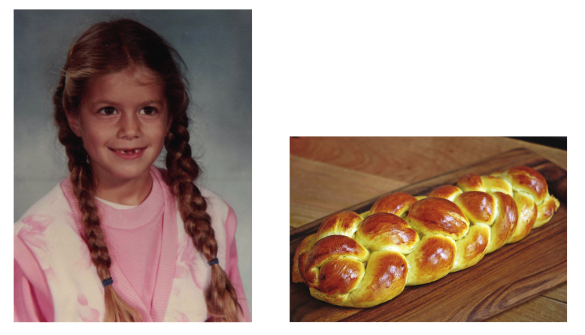
\includegraphics[width=6.1cm]{Images/exemplos_trancas.png}
		\end{center}
		\caption{Trança francesa (à esquerda) e pão trançado (à direita)}\label{exemplos de trancas}
	\end{figure}
	\par\vspace{0.3cm} Podemos ainda representar as tranças através de diagramas, como mostram os exemplos abaixo.
	
	\begin{figure}[H]
		\captionsetup{justification=centering}
		\begin{center}
			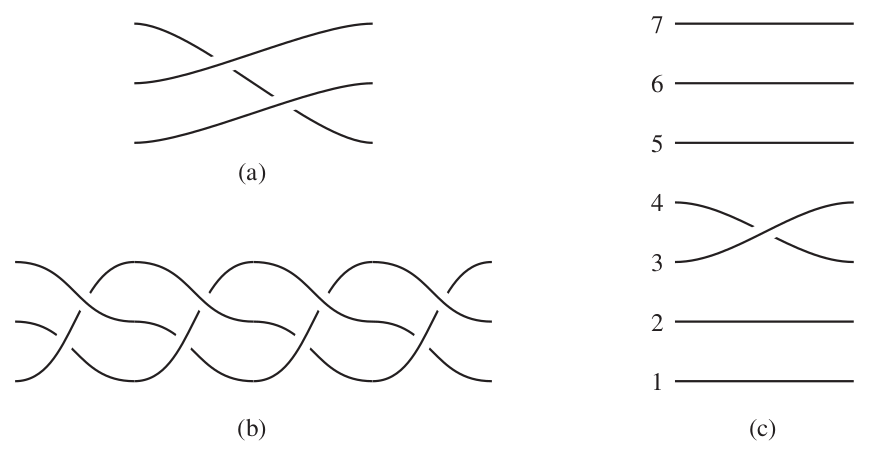
\includegraphics[width=12cm]{Images/exemplos_diagrama.png}
			\caption{
				(a) Uma trança de 3 cordas com 2 cruzamentos \\
				(b) A trança "comum" de 3 cordas (trança francesa) \\
				(c) Corda 3 passa sobre a corda 4
			}\label{diagramas de trancas}\end{center}
	\end{figure}
	
	\par\vspace{0.3cm} Note que cada corda recebe um número (a numeração pode ser feita de cima para baixo ou de baixo para cima). Como dito anteriormente, podemos definir o produto de duas tranças como sendo a concatenação dessas tranças. Além disso, também definimos a trança identidade de maneira bastante intuitiva: ela é apenas o conjunto de $n$ cordas, sem nenhum cruzamento. Veja exemplos abaixo.
	
	\begin{figure}[H]
		\captionsetup{justification=centering}
		\begin{center}
			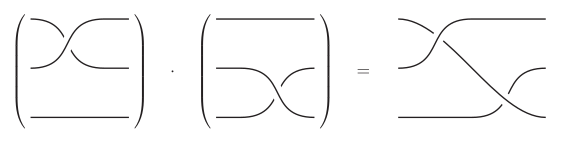
\includegraphics[width=12cm]{Images/produto.png}
		\end{center}\caption{O produto de duas tranças de 3 cordas
		}\label{produto de trancas}
	\end{figure}
	
	\begin{figure}[H]
		\captionsetup{justification=centering}
		\begin{center}
			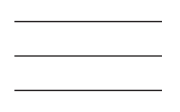
\includegraphics[width=5cm]{Images/identidade_b3.png}
		\end{center}\caption{A identidade em $B_3$}\label{identidade em b3}
	\end{figure}
	
	\begin{figure}[H]
		
		\captionsetup{justification=centering}
		\begin{center}
			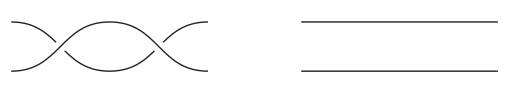
\includegraphics[width=10cm]{Images/identidade_b2.png}
		\end{center}\caption{Duas representações para a identidade em $B_2$. Apesar de parecerem diferentes à primeira vista, elas pertencem à mesma classe de equivalência, ou seja, são a mesma trança em $B_n$}\label{identidade b2}
	\end{figure}
	
	\par\vspace{0.3cm} Definido o produto da forma acima, o que significa ter o inverso de uma trança? Por exemplo, qual seria o inverso da trança $\alpha$ na Figura \eqref{diagramas de trancas}(b)?. Bom, para saber isso devemos, primeiro, conhecer a identidade em $B_3$, que é mostrada acima.
	
	\par\vspace{0.3cm} Bom, como poderíamos estender $\alpha$ para fazê-la parecer a identidade? É impossível: $\alpha$ tem cruzamentos, e desenhar mais coisas não vai mudar isso. Precisamos de uma maneira de cancelar cruzamentos, de modo que as duas tranças na Figura \eqref{identidade b2} sejam equivalentes. 
	
	\par\vspace{0.3cm} Para isso, a ideia é que devemos ser capazes de mover as tranças do mesmo modo que fazemos no espaço (ou seja, sem passar nenhuma corda por dentro de outra) e obter uma trança equivalente. Para definir equivalência, é necessário dizer que quando movemos as tranças, as extremidades devem ficar fixas (do contrário, qualquer trança seria equivalente à identidade).
	
	\par\vspace{0.3cm} Podemos ainda imaginar que as extremidades da esquerda de cada trança estão presas à parede vertical $x=0$ no espaço tridimensional e as extremidades da direita estão presas à parede $x=1$. Nessa configuração, duas tranças são ditas \textit{equivalentes} se podemos mover uma delas, mantendo-a entre as paredes e com as extremidades fixas, e fazê-la parecer a outra. 
	
	\par\vspace{0.3cm} Com essa definição, as duas últimas tranças da Figura \eqref{identidade b2} são equivalentes, assim como as tranças abaixo.
	
	\begin{figure}[H]
		\captionsetup{justification=centering}
		\begin{center}
			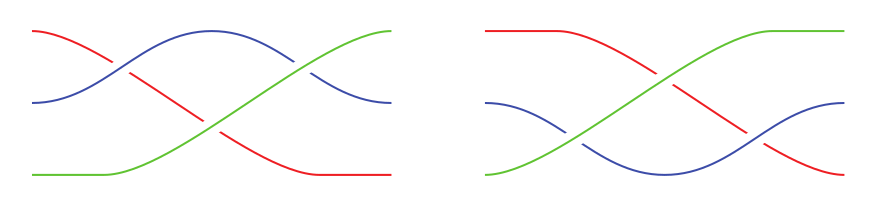
\includegraphics[width=12cm]{Images/fig_18_6.png}
		\end{center}\caption{Duas tranças equivalentes}\label{trancas equivalentes}
	\end{figure}   
	
	\par\vspace{0.3cm} Apenas um aspecto técnico: se fixarmos as paredes que limitam as tranças como sendo $x = 0$ e $x=1$, devemos tomar mais cuidado com o que significa multiplicar duas tranças. Especificamente, para formar $\beta$ vezes $\beta'$, devemos transladar $\beta'$ uma unidade no eixo $x$, tomar a união de $\beta$ com a versão transladada de $\beta'$ e redimensionar tudo por um fator de $1/2$. Isso torna o produto de duas tranças em uma trança.
	
	\par\vspace{0.3cm} Desse modo, note que se fizermos o produto de uma trança $\gamma$ qualquer pela segunda trança da Figura \eqref{identidade b2}, seja à esquerda ou à direita, não alteraremos o número de cruzamentos nem sua configuração, ou seja, não alteraremos a trança $\gamma$. Portanto, de fato, a segunda trança da Figura \eqref{identidade b2} é a identidade em $B_2$.
	
	\par\vspace{0.3cm} Note também que para obter o inverso de uma trança $\alpha$, basta espelharmos $\alpha$, ou seja, o inverso de uma trança qualquer $\alpha$, denotado por $\alpha^{-1}$, nada mais é que a imagem espelhada de $\alpha$.   
	
	
	%\begin{exercise}
	%\label{exercicio 1 tranca}
	%(a) Se convença de que a segunda trança da Figura \eqref{identidade b2} é de fato a identidade em relação ao produto. \\
	
	%(b) Encontre uma trança $\beta$ tal que $\alpha$ (Figura \eqref{diagramas de trancas}(b)) vezes $\beta$ é igual (equivalente) à identidade. \\
	
	%(c) Descreva um procedimento geral para construir o inverso de uma trança.
	%\end{exercise}
	
	%\begin{solution}
	%	(a) Se fizermos o produto de qualquer trança $\gamma$ pela segunda trança da Figura \eqref{identidade b2}, seja à esquerda ou à direita, não alteraremos o número de cruzamentos nem sua configuração, ou seja, não alteraremos nada na trança. \\
	
	%	(b) $\beta$ nada mais é do que $\alpha$ refletida em um espelho. (Introduziremos mais à frente uma notação que nos permitirá representar tranças apenas com símbolos. Nessa notação, $\alpha = (\sigma_1\sigma_2^{-1})^4$ e $\beta = (\alpha)^{-1} = (\sigma_2\sigma_1^{-1})^4$ \\
	
	%	(c) Análogo ao item anterior: basta espelhar a trança desejada.
	%\end{solution}
	
	\par\vspace{0.3cm} 
	
	\begin{remark}
		Nesse sentido, encontrar o inverso de uma trança é parecido com encontrar o inverso de uma matriz: devemos ir "desfazendo" a trança, de trás para frente (da direita para a esquerda), assim como o inverso de um produto $ABC$ de matrizes é dado por $(ABC)^{-1} = C^{-1}B^{-1}A^{-1}$.
	\end{remark}
	
	\par\vspace{0.3cm} 
	
	\begin{lemma}
		\label{B_n grupo}
		Mostre que, para $n$ fixo, as (classes de equivalência de) tranças de $n$ cordas forma um grupo.
	\end{lemma}
	
	\begin{proof}
		A identidade é evidente: ela é apenas o conjunto de n cordas, sem nenhum cruzamento. Anteriormente, enunciamos um procedimento para construir o inverso de uma trança (inverso esse que também é uma trança), logo toda trança possui inverso (inverso esse que também é uma trança). A concatenação (que nada mais é que o produto) de duas tranças de $n$ cordas nos dá outra trança também de $n$ cordas (como vimos anteriormente), logo o conjunto é fechado para o produto. Por fim, a associatividade pode ser verificada através de um diagrama, como o da Figura \eqref{associatividade de trancas}.
		
		\begin{figure}[H]
			\captionsetup{justification=centering}
			\begin{center}
				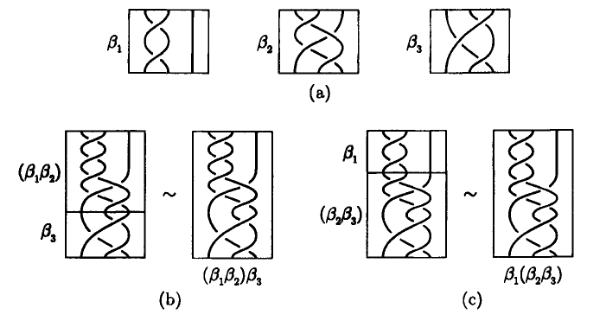
\includegraphics[width=7.1cm]{Images/associatividade.png}
			\end{center}\caption{Associatividade do produto de tranças}\label{associatividade de trancas}
		\end{figure}
	\end{proof}
	\par\vspace{0.3cm} Quando estamos desenhando uma trança, podemos sempre usar a equivalência para evitar que três ou mais cordas se cruzem no mesmo ponto do desenho. Também podemos fazer com que nenhum cruzamento ocorra diretamente acima de outro, como mostra a Figura abaixo.
	
	\begin{figure}[H]
		\captionsetup{justification=centering}
		\begin{center}
			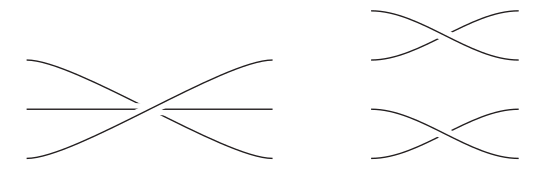
\includegraphics[width=12cm]{Images/desenhos_evitaveis.png}
		\end{center}\caption{Podemos evitar fazer desenhos como esses}\label{diagramas indesejaveis}
	\end{figure}
	
	\par\vspace{0.3cm} Por conta disso, podemos sempre "cortar" qualquer trança, usando linhas verticais, de modo que cada pedaço seja uma trança que contenha somente um cruzamento, como abaixo.
	
	\begin{figure}[H]
		\captionsetup{justification=centering}
		\begin{center}
			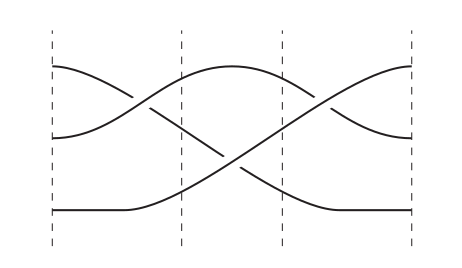
\includegraphics[width=8.6cm]{Images/fig_18_8.png}
		\end{center}\caption{Uma trança como produto de cruzamentos}\label{cortar trancas}
	\end{figure} 
	
	\par\vspace{0.3cm} Em outras palavras, $B_n$ é gerado pelo conjunto de todas as tranças de $n$ cordas que têm exatamente um cruzamento. A trança em que a corda $i$ passa por cima da corda $i+1$ é usualmente denotada por $\sigma_i$. Por exemplo, a Figura \eqref{diagramas de trancas}(c) mostra a trança $\sigma_3$ em $B_7$. O seu inverso seria $\sigma_3^{-1}$, a corda 3 passando por baixo da corda 4. Em geral, a trança em que a corda $i$ passa por baixo da corda $i+1$ (ou, equivalentemente, a corda $i+1$ passa por cima da corda $i$) é denotada por $\sigma_i^{-1}$. 
	
	\par\vspace{0.3cm} Agora, podemos ver que $B_n$ é gerado pelo conjunto $ \{ \sigma_1, \dots, \sigma_{n-1} \} $. Note, porém, que a notação $\sigma_i$ não diz em que grupo de trança estamos, exceto que deve ser pelo menos $B_{i+1}$. Por exemplo, o cruzamento $\sigma_2$ é um gerador de $B_3$, mas também de $B_4$, $B_5$ e assim por diante. O contexto geralmente deixa claro em qual grupo de tranças estamos. 
	
	\par\vspace{0.3cm} Tendo isso em mente, podemos escrever algumas das tranças vistas anteriormente em termos dos geradores $\sigma_i$. Por exemplo, as tranças (a), (b) e (c) da Figura \eqref{diagramas de trancas} podem ser escritas, respectivamente, como $\sigma_2\sigma_1$, $(\sigma_1\sigma_2^{-1})^4$ e $\sigma_3$; a trança da Figura \eqref{produto de trancas} pode ser escrita como $\sigma_2\sigma_1^{-1}$; tanto a trança da Figura \eqref{identidade em b3} quanto a trança da Figura \eqref{identidade b2} são a identidade em seus respectivos grupos ($B_3$ e $B_2$), podendo ser denotadas por $e$ ou, para evitar confusões, $1_3$ e $1_2$, respectivamente (de modo geral, podemos denotar a identidade em $B_n$ por $1_n$); a trança da Figura \eqref{trancas equivalentes} pode ser escrita como $\sigma_1\sigma_2\sigma_1$ ou também como $\sigma_2\sigma_1\sigma_2$. Mais à frente veremos que esse fato não é coincidência, mas uma relação muito importante para o grupo de trança.
	
	%\begin{exercise}
	%	Escreva cada uma das tranças vistas anteriormente como produto de $\sigma_i$ e seus inversos.
	%\end{exercise}
	
	%\begin{solution}
	%	Figura \eqref{diagramas de trancas}(a): $\sigma_2\sigma_1$ \\
	%	Figura \eqref{diagramas de trancas}(b): $(\sigma_1\sigma_2^{-1})^4$ \\
	%	Figura \eqref{diagramas de trancas}(c): $\sigma_3$ \\
	%	Figura \eqref{produto de trancas}: $\sigma_2\sigma_1^{-1}$ \\
	%	Figura \eqref{identidade em b3}: $e$ (em $B_3$) \\
	%	Figura \eqref{identidade b2}: $e$ (em $B_2$) \\
	%	Figura \eqref{trancas equivalentes}: $\sigma_2\sigma_1\sigma_2$ e $\sigma_1\sigma_2\sigma_1$ %(esquerda e direita, respectivamente) 
	%\end{solution}
	
	\par\vspace{0.3cm} Queremos agora pensar sobre como os diferentes $\sigma_i$ se relacionam. Note que se $\sigma_i$ e $\sigma_j$ envolvem cordas completamente distintas, então eles comutam, como ilustrado abaixo.
	
	\begin{figure}[H]
		\captionsetup{justification=centering}
		\begin{center}
			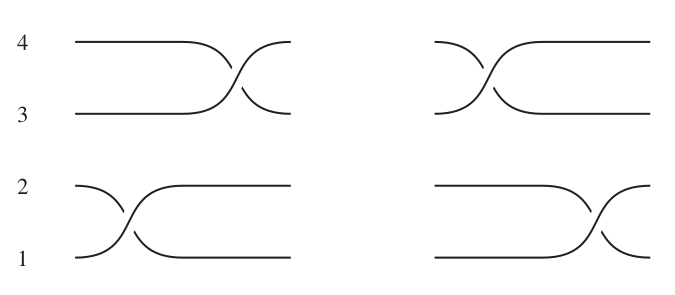
\includegraphics[width=10cm]{Images/comutatividade.png}
		\end{center}\caption{$\sigma_1\sigma_3$ e $\sigma_3\sigma_1$ são equivalentes.}\label{comutatividade de trancas}
	\end{figure}
	
	\par\vspace{0.3cm}
	
	\begin{remark}
		Intuitivamente, se dois cruzamentos envolvem cordas completamente distintas, então podemos "deslizá-los" livremente. Daí vem a comutatividade.
	\end{remark}
	
	\par\vspace{0.3cm} É natural pensar, então, que se dois cruzamentos têm uma corda em comum, então a comutatividade não deve valer. De fato, isso é demonstrado pelo seguinte lema.
	
	\begin{lemma}
		\label{vizinhos nao comutam}
		Dado $B_n$ e $\sigma_i$ um gerador de $B_n$, com $1\leq i\leq n-1$, os cruzamentos vizinhos não comutam, isto é, $\sigma_i\sigma_{i+1}\neq\sigma_{i+1}\sigma_i$.
	\end{lemma}
	
	\begin{proof}
		Basta fazer o desenho, como o do diagrama abaixo.%\eqref{trancas vizinhas nao comutam}.
		
		\begin{center}
			\begin{tikzpicture}
			\braid[braid colour=black,strands=3,braid start={(0,0)}]	{\sigma_1\sigma_2}
			\node[font=\Huge] at (4.5,-1.0) {\(\neq\)};
			\braid[strands=3,braid start={(5,0)}]
			{\sigma_2\sigma_1}
			\end{tikzpicture}
		\end{center}
		
		\par\vspace{0.3cm} Note que não é possível deslizar os cruzamentos de uma das tranças para obter a outra e, consequentemente, cruzamentos vizinhos não comutam. 
		
		%\begin{figure}[H]
		%	\captionsetup{justification=centering}
		%	\begin{center}
		%		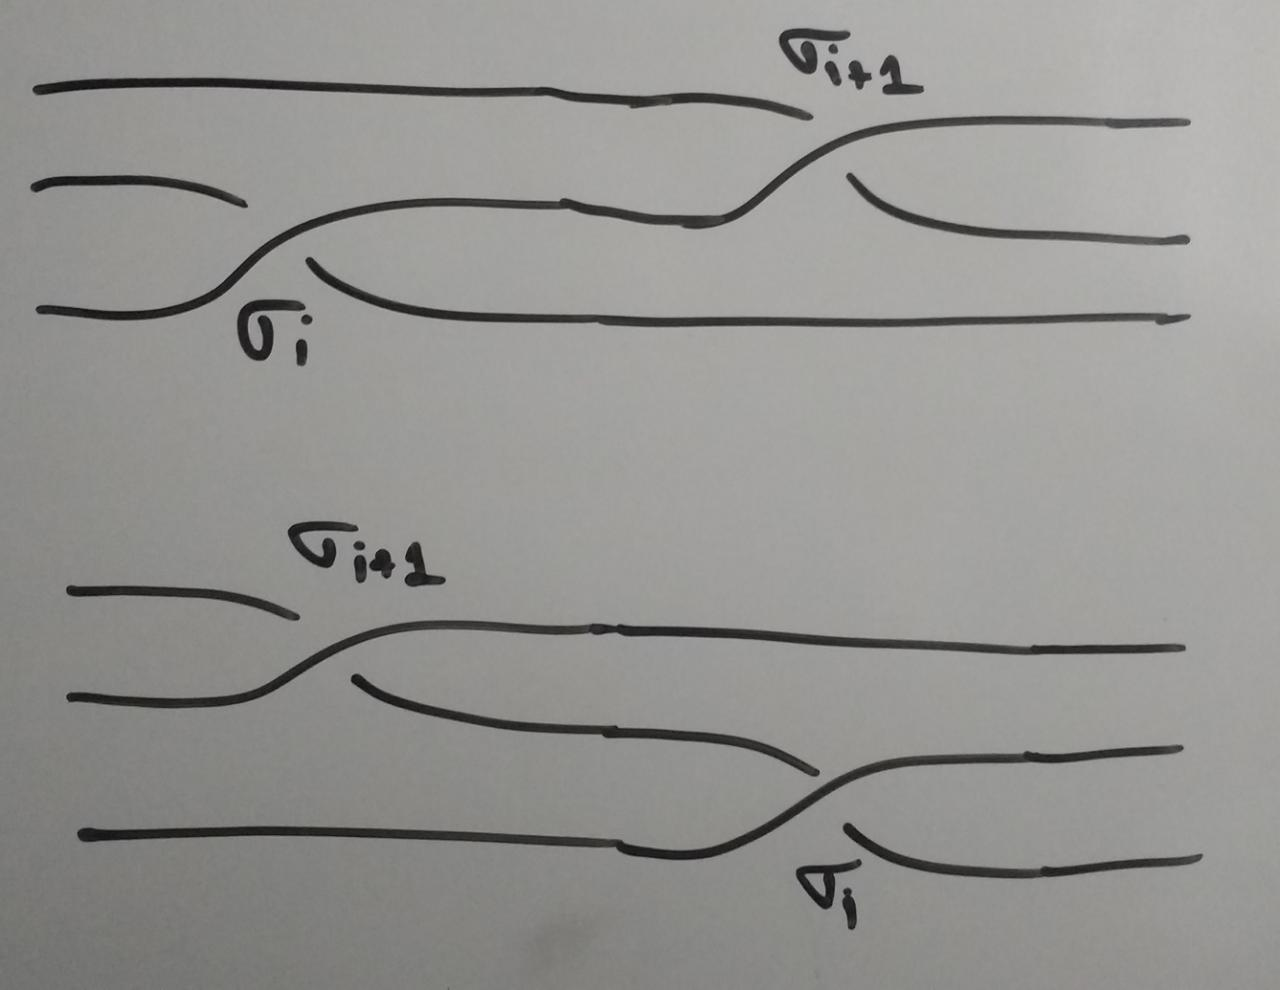
\includegraphics[width=6.4cm]{Images/trancas_vizinhas_nao_comutam.jpeg}
		%	\end{center}\caption{$\sigma_i\sigma_{i+1}\neq\sigma_{i+1}\sigma_i$}\label{trancas vizinhas nao comutam}		
		%\end{figure}
	\end{proof}
	
	\par\vspace{0.3cm} Contudo, os $\sigma_i$'s vizinhos satisfazem a seguinte relação, chamada \textit{relação de trança}:
	
	\begin{equation*}
	\sigma_i\sigma_{i+1}\sigma_i = \sigma_{i+1}\sigma_i\sigma_{i+1}
	\end{equation*}
	
	\par\vspace{0.3cm} 
	
	\begin{lemma}
		Em $B_n$, $\sigma_i\sigma_{i+1}\sigma_i = \sigma_{i+1}\sigma_i\sigma_{i+1}$, para todo $1\leq i\leq n-1$. 
	\end{lemma}
	
	\begin{proof}
		Basta olhar o diagrama abaixo.%\eqref{relacao de tranca}.
		
		\begin{center}
			\begin{tikzpicture}
			\braid[braid colour=black,strands=3,braid start={(0,0)}]	{\sigma_1\sigma_2\sigma_1}
			\node[font=\Huge] at (4.5,-1.5) {\(=\)};
			\braid[strands=3,braid start={(5,0)}]
			{\sigma_2\sigma_1\sigma_2}
			\end{tikzpicture}
		\end{center}
		\par\vspace{0.3cm} Note que podemos obter o diagrama da direita a partir do diagrama da esquerda da seguinte forma: a corda $i$ (à esquerda) é puxada um pouco para baixo; a corda $i+1$ (centro) é puxada para a direita; e a corda $i+2$ (à direita) é puxada um pouco para cima.
		\par\vspace{0.3cm} Então, de fato $\sigma_i\sigma_{i+1}\sigma_i = \sigma_{i+1}\sigma_i\sigma_{i+1}$ para todo $1\leq i\leq n-1$, como queríamos demonstrar.
		%\begin{figure}[H]
		%	\captionsetup{justification=centering}
		%	\begin{center}
		%		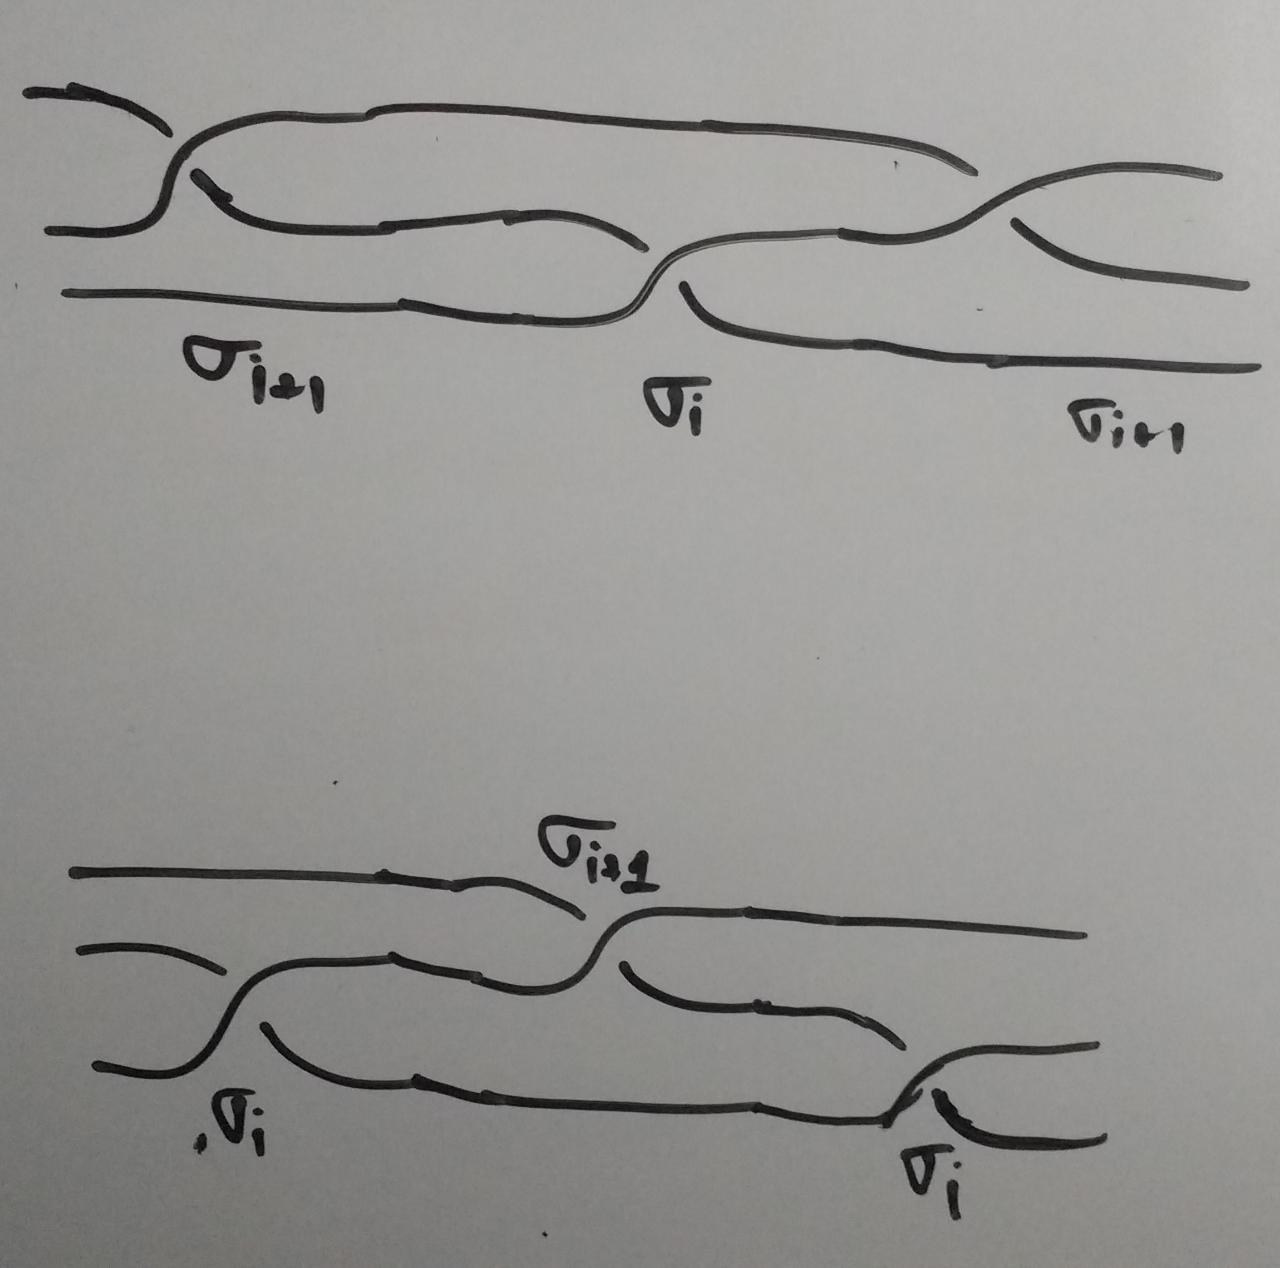
\includegraphics[width=6.4cm]{Images/braid_relation.jpeg}
		%	\end{center}\caption{A relação fundamental das tranças}\label{relacao de tranca}
		%\end{figure}
	\end{proof}
	%
	\par\vspace{0.3cm} Essas duas relações, a comutatividade e a relação de trança, implicam todas as outras relações entre os $\sigma_i$. Em outras palavras:
	
	\begin{theorem}
		\label{apresentacao de B_n}
		O grupo de trança tem a apresentação
		\begin{equation*}
		B_n = \langle \sigma_1, \dots, \sigma_{n-1} | \sigma_i\sigma_j = \sigma_j\sigma_i, \text{ para } |i - j|>1, \\ 
		\sigma_i\sigma_{i+1}\sigma_i = \sigma_{i+1}\sigma_i\sigma_{i+1}, \text{ para } 1\leq i\leq n-2 \rangle
		\end{equation*}
	\end{theorem}
	
	\par\vspace{0.3cm} Aceitaremos o Teorema \eqref{apresentacao de B_n} sem demonstração.
	
	\par\vspace{0.3cm} As duas relações do Teorema \eqref{apresentacao de B_n} nos ajudam a simplificar e manipular palavras em $B_n$. Por exemplo, sabendo que $[a,b] = a^{-1}b^{-1}ab$, podemos manipular $(\sigma_i\sigma_{i+1})^{-1}[\sigma_{i+2}\sigma_i^{-1}, \sigma_i\sigma_{i+1}^{-1}]\sigma_i\sigma_{i+1}$ para obter $\sigma_{i+2}\sigma_i^{-1}$ da seguinte forma:
	\begin{align*}
	&(\sigma_i\sigma_{i+1})^{-1}[\sigma_{i+2}\sigma_i^{-1}, \sigma_i\sigma_{i+1}^{-1}]\sigma_i\sigma_{i+1} \\ 
	&= \sigma_{i+1}^{-1}\sigma_i^{-1}\sigma_i\sigma_{i+2}^{-1}\sigma_{i+1}\sigma_i^{-1}\sigma_{i+2}\sigma_{i+1}^{-1}\sigma_i\sigma_{i+1}  \\
	&= (\sigma_{i+1}^{-1}\sigma_{i+2}^{-1}\sigma_{i+1})\sigma_i^{-1}\sigma_{i+2}(\sigma_{i+1}^{-1}\sigma_i\sigma_{i+1})
	\end{align*}
	
	\par\vspace{0.3cm} Usando a relação de trança, deduzimos a seguinte relação:
	\begin{align*}
	\sigma_i^{-1}\sigma_{i+1}^{-1}\sigma_i = \sigma_{i+1}\sigma_i^{-1}\sigma_{i+1}^{-1} \\
	\sigma_{i+1}^{-1}\sigma_i\sigma_{i+1} = \sigma_i\sigma_{i+1}\sigma_i^{-1}   
	\end{align*}
	
	\par\vspace{0.3cm} Usando essa igualdade, temos
	\begin{align*}
	&(\sigma_{i+1}^{-1}\sigma_{i+2}^{-1}\sigma_{i+1})\sigma_i^{-1}\sigma_{i+2}(\sigma_{i+1}^{-1}\sigma_i\sigma_{i+1}) \\
	&= (\sigma_{i+2}\sigma_{i+1}^{-1}\sigma_{i+2}^{-1})\sigma_i^{-1}\sigma_{i+2}(\sigma_i\sigma_{i+1}\sigma_i^{-1}) \\
	&= \sigma_{i+2}\sigma_{i+1}^{-1}\sigma_{i+2}^{-1}\sigma_i^{-1}\sigma_i\sigma_{i+2}\sigma_{i+1}\sigma_i^{-1} \\
	&= \sigma_{i+2}\sigma_i^{-1}.
	\end{align*}
	
	%\begin{exercise}
	%	Verifique a identidade
	%	\begin{align*}
	%	\sigma_{i+2}\sigma_i^{-1} = (\sigma_i\sigma_{i+1})^{-1}[\sigma_{i+2}\sigma_i^{-1}, \sigma_i\sigma_{i+1}^{-1}]\sigma_i\sigma_{i+1}
	%	\end{align*}
	%	\par\vspace{0.3cm} sendo $1\leq i\leq n-3$ e $[a,b] = a^{-1}b^{-1}ab$.
	
	%\end{exercise}
	
	%\begin{solution}
	%	Vamos manipular o lado direito. Temos
	
	%	\begin{align*}
	%	&(\sigma_i\sigma_{i+1})^{-1}[\sigma_{i+2}\sigma_i^{-1}, \sigma_i\sigma_{i+1}^{-1}]\sigma_i\sigma_{i+1} \\ 
	%	&= \sigma_{i+1}^{-1}\sigma_i^{-1}\sigma_i\sigma_{i+2}^{-1}\sigma_{i+1}\sigma_i^{-1}\sigma_{i+2}\sigma_{i+1}^{-1}\sigma_i\sigma_{i+1}  \\
	%	&= (\sigma_{i+1}^{-1}\sigma_{i+2}^{-1}\sigma_{i+1})\sigma_i^{-1}\sigma_{i+2}(\sigma_{i+1}^{-1}\sigma_i\sigma_{i+1})
	%	\end{align*}
	
	%	\par\vspace{0.3cm} Da relação $\sigma_i\sigma_{i+1}\sigma_i = \sigma_{i+1}\sigma_i\sigma_{i+1}$, obtemos que
	
	%	\begin{align*}
	%	\sigma_i^{-1}\sigma_{i+1}^{-1}\sigma_i = \sigma_{i+1}\sigma_i^{-1}\sigma_{i+1}^{-1} \\
	%	\sigma_{i+1}^{-1}\sigma_i\sigma_{i+1} = \sigma_i\sigma_{i+1}\sigma_i^{-1}   
	%	\end{align*}
	
	%	\par\vspace{0.3cm} Substituindo acima, segue
	
	%	\begin{align*}
	%	&(\sigma_{i+1}^{-1}\sigma_{i+2}^{-1}\sigma_{i+1})\sigma_i^{-1}\sigma_{i+2}(\sigma_{i+1}^{-1}\sigma_i\sigma_{i+1}) \\
	%	&= (\sigma_{i+2}\sigma_{i+1}^{-1}\sigma_{i+2}^{-1})\sigma_i^{-1}\sigma_{i+2}(\sigma_i\sigma_{i+1}\sigma_i^{-1}) \\
	%	&= \sigma_{i+2}\sigma_{i+1}^{-1}\sigma_{i+2}^{-1}\sigma_i^{-1}\sigma_i\sigma_{i+2}\sigma_{i+1}\sigma_i^{-1} \\
	%	&= \sigma_{i+2}\sigma_i^{-1}.
	%	\end{align*}
	
	%	\par\vspace{0.3cm} que conclui a verificação.
	%\end{solution}
	
	\par\vspace{0.3cm} Outra aplicação do Teorema \eqref{apresentacao de B_n} é o fato de que $B_2\cong\mathbb{Z}$. Para perceber isso, basta notar que pelo Teorema \eqref{apresentacao de B_n}, $B_2 = \langle \sigma_1 | - \rangle$ e $\mathbb{Z}$ tem essa mesma apresentação. 
	
	\par\vspace{0.3cm} Também com o Teorema \eqref{apresentacao de B_n}, podemos escrever $B_3 = \langle \sigma_1,\sigma_2 | \sigma_1\sigma_2\sigma_1 = \sigma_2\sigma_1\sigma_2 \rangle$ e, com isso, mostrar que $B_3 \cong\langle x,y | x^3=y^2 \rangle$ da seguinte maneira.
	
	\par\vspace{0.3cm} Da apresentação $B_3 = \langle \sigma_1,\sigma_2 | \sigma_1\sigma_2\sigma_1 = \sigma_2\sigma_1\sigma_2 \rangle$, podemos obter a relação equivalente $(\sigma_1\sigma_2)^3 = (\sigma_2\sigma_1\sigma_2)^2 = (\sigma_1\sigma_2\sigma_1)^2$. Daí, usando o Lema \eqref{lema geradores}, sabemos que $\langle \sigma_1,\sigma_2 \rangle = \langle \sigma_1\sigma_2,\sigma_2 \rangle = \langle \sigma_1\sigma_2, \sigma_2\sigma_1 \rangle = \langle \sigma_1\sigma_2, \sigma_1\sigma_2\sigma_1 \rangle$. Portanto, fazendo $x = \sigma_1\sigma_2$ e $y = \sigma_1\sigma_2\sigma_1$, concluímos que $B_3 \cong \langle x,y | x^3=y^2 \rangle$.
	
	%\begin{exercise}
	%	\label{outra apresentacao de B_3}
	%	(a) Usando o Teorema \eqref{apresentacao de B_n}, mostre que $B_2\cong\mathbb{Z}$. \\
	
	%	(b) Usando o Teorema \eqref{apresentacao de B_n}, escreva uma apresentação para $B_3$. \\
	
	%	(c) Mostre que $B_3\cong\langle x,y | x^3 = y^2 \rangle$.
	%\end{exercise}
	
	%\begin{solution}
	%	(a) Do Teorema \eqref{apresentacao de B_n}, $B_2 = \langle \sigma_1|- \rangle$, ou seja, $B_2$ é gerado por um elemento e não possui nenhuma relação, assim como $\mathbb{Z}$. Logo, eles são isomorfos. Podemos enxergar $\sigma_1$ como sendo equivalente a somar $1$ e $\sigma_1^{-1}$ como somar $-1$.\\
	
	%	(b) Do Teorema \eqref{apresentacao de B_n}, temos $B_3 = \langle \sigma_1, \sigma_2 | \sigma_1\sigma_2\sigma_1 = \sigma_2\sigma_1\sigma_2 \rangle$. \\
	
	%	(c) Da apresentação do item (b), sabemos que os geradores de $B_3$ satisfazem a relação $\sigma_1\sigma_2\sigma_1=\sigma_2\sigma_1\sigma_2$. Isso é equivalente a $(\sigma_1\sigma_2)^3=(\sigma_2\sigma_1\sigma_2)^2=(\sigma_1\sigma_2\sigma_1)^2$. Daí, usando o fato de que $\langle a,b\rangle=\langle a,ab\rangle$, também sabemos que $B_3$ é gerado por $\langle \sigma_1\sigma_2,\sigma_2\rangle=\langle \sigma_1\sigma_2,\sigma_2\sigma_1\rangle=\langle \sigma_1\sigma_2,\sigma_1\sigma_2\sigma_1\rangle$. Portanto, fazendo $x=\sigma_1\sigma_2$ e $y=\sigma_1\sigma_2\sigma_1$, concluímos que $B_3=\langle x,y|x^3=y^2\rangle$.
	%\end{solution}
	
	\par\vspace{0.3cm}
	
	\begin{remark}
		Um fato interessante é que como $SL(2,\mathbb{Z}) = \langle s,t | s^3 = t^2, t^4 = 1 \rangle$ (não será demonstrado), e $B_3 = \langle x,y| x^3 = y^2 \rangle$, podemos ver que o conjunto de relações de $B_3$ está contido no conjunto de relações de $SL(2,\mathbb{Z})$. Consequentemente, pelo Teorema \eqref{teorema de Dyck}, $SL(2,\mathbb{Z})$ é imagem homomórfica de $B_3$, i.e., $B_3$ é homomorfo a $SL(2,\mathbb{Z})$. 
	\end{remark}
	
	\par\vspace{0.3cm}
	
	\begin{lemma}
		\label{homomorfismo de comprimento}
		Defina a função $l$, chamada homomorfismo de comprimento, de $B_n$ para os inteiros da seguinte forma: Se $w$ é uma palavra nos geradores $\sigma_i$ e seus inversos, faça $l(w)$ ser a soma dos expoentes dos $\sigma_i$ em $w$. Em outras palavras, cada $\sigma_i$ conta como $1$ e cada $\sigma_i^{-1}$ conta como $-1$. Mostre que $l$ está bem definida e é um homomorfismo.
	\end{lemma}
	
	\begin{proof}
		Sejam $w_1,w_2$ duas palavras em $B_n$ tais que $w_1=w_2$. Então, por definição, podemos, após uma quantidade finita de inserções e remoções de elementos da forma $\sigma_i\sigma_i^{-1}$, sair de $w_1$ e chegar em $w_2$. Como cada inserção/remoção desse tipo não altera a soma dos expoentes, pois estamos somando 0, então $l(w_1)=l(w_2)$, i.e., $l$ está bem definida. 
		\par\vspace{0.3cm} Agora, sejam $w_1,w_2$ duas palavras quaisquer em $B_n$. Note que $l(w_1w_2)$ é, por definição, a soma dos expoentes de $w_1w_2$. Mas essa soma nada mais é do que a soma dos expoentes de $w_1$ acrescida à soma dos expoentes de $w_2$, i.e., nada mais é do que $l(w_1)+l(w_2)$. Note que essa igualdade vale ainda que o final de $w_1$ seja o inverso do início de $w_2$ (por exemplo, $w_1 = \cdots\sigma_1\sigma_2^{-1}$ e $w_2 = \sigma_2\sigma_3\cdots$. Nesse caso, $l(w_1w_2)$ continua sendo igual a $l(w_1) + l(w_2)$). Logo, $l(w_1w_2)=l(w_1)+l(w_2)$ e $l$ preserva a operação, sendo portanto, homomorfismo.
		\par\vspace{0.3cm} Por fim, note também que $l$ é sobrejetora, uma vez que dado $n\in\mathbb{Z}$, podemos tomar a palavra $w = \underbrace{\sigma_1\sigma_1\cdots\sigma_1}_{n}$ de forma a obter $l(w) = n$.
	\end{proof}
	
	\begin{remark}
		A função $l$ do Lema \eqref{homomorfismo de comprimento} é bem útil na verificação de equivalência entre duas tranças. Isso porque a função $l$ é um invariante no grupo de tranças, i.e, se duas tranças são equivalentes, suas imagens por $l$ (expoentes) devem ser iguais (segue da boa definição de $l$). Daí, podemos usar a contrapositiva: se duas tranças têm expoentes diferentes, então elas não podem ser equivalentes.
	\end{remark}
	
	\par\vspace{0.3cm} Da definição de $l$, é imediato que dada uma palavra $w$ qualquer, $l(w^{-1}) = -l(w)$.
	
	\par\vspace{0.3cm} Uma aplicação interessante de $l$ é a seguinte: se $\gamma$ é uma trança qualquer conjugada ao seu inverso, i.e., se existe um trança $\delta$ tal que $\delta\gamma\delta^{-1} = \gamma^{-1}$, então $l(\gamma) = 0$.
	
	\par\vspace{0.3cm} De fato, se $\gamma$ é conjugada ao seu inverso, sabemos que $l(\delta\gamma\delta^{-1}) = l(\gamma^{-1})$. Pela definição de $l$, temos que $l(\delta\gamma\delta^{-1}) = l(\gamma)$. Daí, $l(\gamma) = l(\gamma^{-1}) = -l(\gamma)$ e, consequentemente, $l(\gamma) = 0$.
	
	%\begin{exercise}
	%	(a) Mostre que os geradores $\sigma_i$ de $B_n$ são conjugados uns dos outros.\\
	
	%	(b) Sejam $\delta=\sigma_1\sigma_2\sigma_1$ e $\gamma=\sigma_2\sigma_1^{-1}$. Mostre que $\delta\gamma\delta^{-1}=\gamma^{-1}$. Então o grupo de tranças contém um elemento $\gamma$ que é conjugado ao próprio inverso.\\
	
	%	(c) Mostre que se $\gamma$ é qualquer trança que é conjugada ao próprio inverso, então $l(\gamma)=0$.
	%\end{exercise}
	
	%\begin{proof}
	%	(a) Sabemos que $\sigma_i\sigma_{i+1}\sigma_i=\sigma_{i+1}\sigma_i\sigma_{i+1}$, para $1\leq i\leq n-2$. Isso é equivalente a $(\sigma_i\sigma_{i+1})\sigma_i(\sigma_i\sigma_{i+1})^{-1}=\sigma_{i+1}$, logo $\sigma_i$ é conjugado de $\sigma_{i+1}$.\\
	
	%	(b) Note que $\delta\gamma^{-1}\delta^{-1}=(\sigma_1\sigma_2\sigma_1)(\sigma_2\sigma_1^{-1})(\sigma_1^{-1}\sigma_2^{-1}\sigma_1^{-1})=(\sigma_1\sigma_1\sigma_2)(\sigma_2^{-1}\sigma_1^{-1}\sigma_2^{-1})=\sigma_1\sigma_2^{-1}=\gamma^{-1}$.\\
	
	%	(c) Se $\gamma$ é conjugada ao seu inverso, então $\delta\gamma\delta^{-1}=\gamma^{-1}$, para algum $\delta$. Daí, note que $l(\delta\gamma\delta^{-1})=l(\gamma^{-1})\Rightarrow l(\gamma)=-l(\gamma)\Rightarrow l(\gamma)=0.$
	%\end{proof}
	
	\par\vspace{0.3cm} Podemos, ainda, pensar em tranças em termos de permutações, no sentido de que existe um mapa $\pi: B_n\to S_n$ em que tomamos uma trança, ignorando se os cruzamentos são por cima ou por baixo, e, numerando as posições inicial e final de cada corda, apenas lemos a permutação correspondente (lembre que $S_n$ se refere ao grupo simétrico).
	
	\par\vspace{0.3cm}
	
	\begin{lemma}
		\label{B_n iso S_n}
		Mostre que $\pi: B_n\to S_n$ é um homomorfismo.
	\end{lemma}
	
	\begin{proof}
		Seja $\psi:\underset{\sigma_i\mapsto(i\text{ }i+1)}{B_n\to S_n}$. Note que $\psi$ está bem definida, uma vez que $\sigma_i=\sigma_j\Rightarrow\psi(\sigma_i)=\psi(\sigma_j)$. Então, sejam $\sigma_i,\sigma_j\in B_n$ quaisquer. Suponha $|i-j|>1$. Então, $\psi(\sigma_i\sigma_j)=(i\text{ } i+1)(j\text{ } j+1)=\psi(\sigma_i)\psi(\sigma_j)$. Se $|i-j|=1$, podemos supor, sem perda de generalidade, que $j=i+1$. Então, temos $\psi(\sigma_i\sigma_{i+1})=(i\text{ } i+2\text{ } i+1)=(i\text{ } i+1)(i+1\text{ } i+2)=\psi(\sigma_i)\psi(\sigma_{i+1})$. Portanto, $\psi$ preserva a operação. 
		\par\vspace{0.3cm} Por fim, note também que $\psi$ é sobrejetora, uma vez que dada uma permutação qualquer, sempre podemos construir uma trança cuja imagem por $\psi$ é tal permutação. Esse argumento será formalizado mais adiante.
	\end{proof}
	
	\par\vspace{0.3cm}
	
	\begin{lemma}
		\label{apresentacao de S_n}
		Considere a seguinte apresentação, que lembra a apresentação do Teorema \eqref{apresentacao de B_n}:
		
		\begin{align*} G = \langle \tau_1,\dots,\tau_{n-1} | &\tau_i\tau_j = \tau_j\tau_i, \text{ para }|i - j|>1,\\ &\tau_i\tau_{i+1}\tau_i = \tau_{i+1}\tau_i\tau_{i+1}, \text{ para } 1\leq i\leq n-2, \\ &\tau_i^2 = 1, \text{ para }1\leq i\leq n-1\rangle. 
		\end{align*}
		
		\par\vspace{0.3cm} Mostre que $S_n\cong G$, ou seja, \begin{align*} S_n = \langle \tau_1,\dots,\tau_{n-1} | &\tau_i\tau_j = \tau_j\tau_i, \text{ para }|i - j|>1,\\ &\tau_i\tau_{i+1}\tau_i = \tau_{i+1}\tau_i\tau_{i+1}, \text{ para } 1\leq i\leq n-2, \\ &\tau_i^2 = 1, \text{ para }1\leq i\leq n-1\rangle. 
		\end{align*}
		
		%(a) Encontre elementos $\tau_i\in S_n$ que satisfaçam tais relações. \\
		
		%(b) Use o item (a) para mostrar que a função levando $\tau_i\in G$ para $\tau_i\in S_n$ se extende para um homomorfismo sobrejetor bem definido de $G$ em $S_n$. \\
		
		%(c) Mostre que esse homomorfismo também é injetivo. Logo, a apresentação acima é a apresentação de $S_n$.
		
	\end{lemma}
	
	\begin{proof}
		Primeiro, note que as transposições $\tau_i$ em $S_n$ satisfazem todas as relações de $G$. Seja $\gamma:\underset{\tau_i\mapsto (i\text{ }i+1)}{G\to S_n}$. A boa definição de $\gamma$ e a propriedade de preservar a operação são demonstradas de maneira análoga ao que foi feito no Lema \eqref{B_n iso S_n}.
		\par\vspace{0.3cm} Então, seja $(i\text{ }i+1)\in S_n$ qualquer e tome $\tau_i\in G$. Daí, $\gamma(\tau_i) = (i\text{ }i+1)$ e, portanto, $\gamma$ é sobrejetora.
		\par\vspace{0.3cm} Por fim, suponha $\gamma(\tau_i) = \gamma(\tau_j)$. Então, $(i\text{ }i+1) = (j\text{ }j+1)$, ou seja, $i = j$, o que é equivalente a $\tau_i = \tau_j$. Portanto, $\gamma$ é injetora e, consequentemente, $\gamma$ é um isomorfismo de $G$ em $S_n$, como queríamos demonstrar.
	\end{proof}
	
	%\begin{solution}
	%	(a) Tais elementos são as transposições $(i\text{ } i+1)$ de dois elementos (cordas) consecutivos. \\
	
	%	(b) Seja $\gamma:\underset{\tau_i\mapsto(i\text{ } i+1)}{G\to S_n}$. A boa definição e a preservação da operação são demonstradas de maneira análoga ao exercício anterior. Por fim, seja $(i\text{ } i+1)\in S_n$ qualquer. Então, tome $\tau_i\in G$. Daí, $\gamma(\tau_i)=(i\text{ } i+1)$ e, portanto, $\gamma$ é sobrejetora. \\
	
	%	(c) Suponha $\gamma(\tau_i)=\gamma(\tau_j)$. Então, $(i\text{ } i+1)=(j\text{ } j+1)$, ou seja, $i=j \Leftrightarrow \tau_i=\tau_j$. Portanto, $\gamma$ é injetora e, consequentemente, $\gamma$ define um isomorfismo de $G$ em $S_n$. Logo, $S_n$ tem a apresentação acima.
	%\end{solution}
	
	\par\vspace{0.3cm} Podemos, ainda, definir uma trança geometricamente, como a seguir.
	
	\begin{deff}
		\label{def geometrica tranca}
		Seja $I = [0,1]$. Uma trança geométrica em $n\geq 1$ cordas é um conjunto $b\subset\mathbb{R}^2\times I$ formado por $n$ intervalos topológicos disjuntos chamados cordas de $b$ tal que a projeção $\mathbb{R}^2\times I\to I$ mapeia cada corda homeomorficamente em $I$ e 
		
		\begin{align*}
		b\cap (\mathbb{R}^2\times \{ 0 \}) &= \left\{ (1,0,0), (2,0,0), \dots, (n,0,0) \right\} \\
		b\cap (\mathbb{R}^2\times \{ 1 \}) &= \left\{ (1,0,1), (2,0,1), \dots, (n,0,1) \right\}.
		\end{align*}
	\end{deff}
	
	\par\vspace{0.3cm} Da Definição \eqref{def geometrica tranca}, podemos ver que cada corda de $b$ intersecta cada plano $\mathbb{R}^2\times\{t\}$, com $t\in I$, em exatamente um ponto. Também vemos que cada corda de $b$ conecta um ponto $(i,0,0)$ a um ponto $(s(i), 0, 1)$, com $i,s(i)\in \{1, 2, \dots, n\}$. A sequência $(s(1), s(2), \dots, s(n))$ é uma permutação do conjunto $\{1, 2, \dots, n\}$ chamada permutação subjacente de $b$.
	
	\begin{remark}
		Apesar de ser técnica, note que o que a Definição \eqref{def geometrica tranca} nos diz algo simples; o que ela está falando é que uma trança é um subconjunto $b$ da região $0\leq z\leq 1 $ de $\mathbb{R}^3$. Além disso, as interseções entre $b$ e os planos $z = 0$ e $z = 1$ são, respectivamente, o conjunto de pontos $\left\{  (1,0,0), \dots, (n,0,0)\right\}$ e o conjunto de pontos $\left\{ (1,0,1), \dots, (n,0,1) \right\}$. Esses dois conjuntos são as extremidades de cada corda da trança.
		
		\par\vspace{0.3cm} Note também que, da Definição \eqref{def informal tranca}, sabemos que as cordas de uma trança não podem passar uma por dentro da outra, ou seja, não podem se interceptar e também sabemos que cada corda deve ir monotonicamente da esquerda para a direita, ou seja, não pode haver loops. A Definição \eqref{def geometrica tranca} respeita essas condições, uma vez que cada plano $\mathbb{R}^2\times\{t\}$, com $t\in [0,1]$, intercepta cada corda de $b$ em exatamente um ponto, logo cada corda vai monotonicamente de cima para baixo, e as cordas de $b$ são disjuntas, isto é, não se interpcetam. Essa última propriedade significa que entre os planos $\mathbb{R}^2\times \{0\}$ e $\mathbb{R}^2\times \{1\}$, o valor da coordenada $y$ varia: começa em $0$, aumenta (em módulo), e retorna a $0$.
	\end{remark}
	
	\par\vspace{0.3cm} Podemos, ainda, reescrever a Definição \eqref{def geometrica tranca} da seguinte forma:
	
	\begin{deff}
		\label{outra def geometrica tranca}
		Seja $n\in\mathbb{N}$ fixo. Sejam ainda $n$ pontos distintos $p_1, \dots, p_n$ em $\mathbb{R}^2$. Seja $(f_1, \dots, f_n)$ uma $n$-upla de funções $f_i:[0,1]\to\mathbb{R}^2$ tais que $f_i(0) = p_i$, $f_i(1) = p_j$ para algum $j=1,\dots,n$ e tais que os $n$ caminhos 
		
		\begin{align*}
		[0,1]&\to\mathbb{R}^2\times[0,1] \\
		t&\mapsto (f_i(t), t)
		\end{align*}
		
		\par\vspace{0.3cm} chamados cordas, tenham imagens disjuntas. Essas $n$ cordas são chamadas de trança. O grupo de trança $B_n$ em $n$ cordas é o grupo de classes de isotopia de tranças. O produto de uma trança $( f_1(t), \dots, f_n(t) )$ por uma trança $( g_1(t), \dots, g_n(t) )$ é definido por
		
		\begin{align}
		\label{def prod trancas}
		(f\bullet g)_i(t) = \begin{cases}
		f_i(2t), 0\leq t\leq \displaystyle{\frac{1}{2}} \\
		g_j(2t-1), \displaystyle{\frac{1}{2}}\leq t\leq 1
		\end{cases}\text{ sendo } j \text{ tal que }f_i(1) = p_j.
		\end{align}
		
	\end{deff}
	
	\par\vspace{0.3cm} O interessante de se observar na Definição \eqref{outra def geometrica tranca} é o modo como o produto de tranças foi apresentado na Definição \eqref{outra def geometrica tranca}. O que a equação \eqref{def prod trancas} nos diz é que para multiplicar a trança $\alpha = ( f_1(t), \dots, f_n(t) )$ pela trança $\beta = ( g_1(t), \dots, g_n(t) )$, devemos diminuir o "tamanho" de ambas as tranças pela metade e, em seguida, conectá-las, colocando $\alpha$ "em cima" de $\beta$. Outra maneira equivalente de pensar é que apenas "encurtamos" $\alpha$ por um fator de $1/2$, sem transladá-la, e "encurtamos" $\beta$ também por um fator de $1/2$, mas transladamos $1/2$ na direção negativa do eixo $\cal{O}z$. Essa definição é a mesma que a Definição \eqref{def informal tranca}, apenas formalizada!
	
	\chapter{Propriedades de $B_n$ e o grupo de tranças puras}
	
	\hspace{12pt} Vamos demonstrar algumas propriedades das tranças. Para evitar confusões, por vezes será usada a notação $1_n$ para indicar a identidade de $B_n$.
	
	%\begin{prop}
	%	\label{centro de B_n}
	%	Para $1\leq i\leq n-1$, $(\sigma_1\sigma_2\cdots\sigma_{n-1})^n\sigma_i = \sigma_i(\sigma_1\sigma_2\cdots\sigma_{n-1})^n$, ou seja, $(\sigma_1\sigma_2\cdots\sigma_{n-1})^n$ pertence ao centro de $B_n$.
	%\end{prop}
	
	%\begin{proof}
	
	%\end{proof}
	
	%\begin{remark}
	%	É possível mostrar que $(\sigma_1\sigma_2\cdots\sigma_{n-1})^n$ gera o centro de $B_n$. Além disso, como $l((\sigma_1\sigma_2\cdots\sigma_{n-1})^n)\neq 0 = l(1_n)$ (sendo $l$ a função definida no Lema \eqref{homomorfismo de comprimento}), então $(\sigma_1\sigma_2\cdots\sigma_{n-1})^n\neq 1_n$ e, consequentemente, o centro de $B_n$ não é trivial.
	%\end{remark}
	
	\begin{prop}
		\label{B_m subgrupo de B_n}
		Para $1\leq m\leq n$, o mapa $\psi: \underset{\sigma_i\mapsto\sigma_i}{B_m\to B_n}$ para $1\leq i\leq m-1$ é um homomorfismo injetor de $B_m$ em $B_n$ e então podemos considerar $B_m$ um subgrupo de $B_n$. 
	\end{prop}
	
	
	\begin{proof}
		Pelo Teorema \eqref{apresentacao de B_n}, temos
		
		\begin{align*}
		B_m = \langle \sigma_1, \sigma_2, \dots, \sigma_{m-1} | &\sigma_i\sigma_j = \sigma_j\sigma_i, \text{ para }|i-j|>1 \\ 
		&\sigma_i\sigma_{i+1}\sigma_i = \sigma_{i+1}\sigma_i\sigma_{i+1}, 1\leq i\leq m-2\rangle \\
		B_n = \langle \sigma_1, \sigma_2, \dots, \sigma_{m-1}, \dots, \sigma_{n-1} | \sigma_i\sigma_j = &\sigma_j\sigma_i, \text{ para }|i-j|>1 \\ 
		&\sigma_i\sigma_{i+1}\sigma_i = \sigma_{i+1}\sigma_i\sigma_{i+1}, 1\leq i\leq n-2\rangle
		\end{align*} 
		
		\par\vspace{0.3cm} Daí, como $B_n$ satisfaz as relações de $B_m$, então pelo Teorema \eqref{teorema de Dyck}, $\psi$ é homomorfismo.
		
		\par\vspace{0.3cm} Agora, suponha que existe $\beta\in B_n$ tal que $\psi(\beta) = 1_n$, ou seja, existe uma trança $\beta$ de $m$ cordas que, quando adicionamos $n-m$ cordas retas, se torna a trança trivial em $B_n$. Mas então devemos ter $\beta = 1_m$, logo $\psi$ é injetora.
		
	\end{proof}
	
	\begin{remark}
		\begin{enumerate}
			\item Como consequência da Proposição \eqref{B_m subgrupo de B_n}, se $\beta\in B_m$ é não trivial, então $\beta\in B_n$, $n\geq m$, também é não trivial (sendo $\beta\in B_n$ a trança $\beta$ de $m$ cordas adicionada de $n-m$ cordas retas).
			\item Outra observação interessante é o fato de que, Em particular, $B_m\cong B_n$ se, e só se, $m=n$.
		\end{enumerate}
	\end{remark}
	
	\begin{prop}
		\label{geradores de B_n tem ordem infinita}
		$B_n$ é \textbf{livre de torção}, i.e., todo gerador de $B_n$ tem ordem infinita. Equivalentemente, $\sigma_i^k \neq 1, \forall k\in\mathbb{Z}^{\ast}$.
	\end{prop}
	
	\begin{proof}
		Vamos demonstrar a Proposição \eqref{geradores de B_n tem ordem infinita} por indução em $i$, o índice dos geradores.	Como $B_2 = \langle \sigma_1 | - \rangle$, então $|\sigma_1| = \infty$. Logo, em $B_n$, $|\sigma_1| = \infty$. Suponha, então, que $\sigma_2\in B_n$ tem ordem finita. Logo, por definição, $\exists l\in\mathbb{Z}$ tal que $\sigma_2^l = 1_n$. Daí, 
		
		\begin{equation*}
		(\sigma_1\sigma_2\sigma_1)\sigma_2^l(\sigma_1\sigma_2\sigma_1)^{-1} = 1_n
		\end{equation*}
		
		\par\vspace{0.3cm} Note que como $\sigma_i\sigma_{i+1}\sigma_i = \sigma_{i+1}\sigma_i\sigma_{i+1}$, então $\sigma_i\sigma_{i+1}\sigma_i^{-1} = \sigma_{i+1}^{-1}\sigma_i\sigma_{i+1}$ e, consequentemente, $\sigma_i\sigma_{i+1}^l\sigma_i^{-1} = \sigma_{i+1}^{-1}\sigma_i^l\sigma_{i+1}$. Substituindo na equação acima, temos
		
		\begin{align*}
		1_n &= \sigma_1\sigma_2\sigma_1\sigma_2^l\sigma_1^{-1}\sigma_2^{-1}\sigma_1^{-1} \\
		&= \sigma_1\sigma_2\sigma_2^{-1}\sigma_1^l\sigma_2\sigma_2^{-1}\sigma_1^{-1} \\
		&= \sigma_1^l
		\end{align*}
		
		\par\vspace{0.3cm} o que é absurdo, logo $|\sigma_2| = \infty$.
		
		\par\vspace{0.3cm} Então, suponha indutivamente que $|\sigma_j| = \infty, 1\leq j\leq i-1$. Suponha que $|\sigma_i| = l, l\in\mathbb{Z}$. Então, 
		
		\begin{align*}
		1_n &= \sigma_{i-1}\sigma_i\sigma_{i-1}\sigma_i^l\sigma_{i-1}^{-1}\sigma_i^{-1}\sigma_{i-1}^{-1} \\
		&= \sigma_{i-1}\sigma_i\sigma_i^{-1}\sigma_{i-1}^l\sigma_i\sigma_i^{-1}\sigma_{i-1}^{-1} \\
		&= \sigma_{i-1}^l
		\end{align*}
		
		\par\vspace{0.3cm} o que é absurdo também. Então, por indução, $|\sigma_i| = \infty, i\geq 1$. 
	\end{proof}
	
	\begin{remark}
		Como todo elemento não trivial de $B_n$ tem ordem infinita, é possível mostrar que para toda trança $\beta$ não trivial de $B_n$, $\beta^k\neq 1_n$ se $k\neq 0$.
	\end{remark}
	
	\begin{prop}
		\label{sigma1 e alfa geram B_n}
		O grupo $B_n$, $n\geq 1$, é gerado pelos elementos $\sigma_1$ e $\alpha = \sigma_1\sigma_2\cdots\sigma_{n-1}$.
	\end{prop}
	
	\begin{proof}
		Queremos obtes os $\sigma_i$, $i\geq 2$, em termos de $\sigma_1$ e $\alpha$. Primeiro, vamos mostrar que 
		
		\begin{equation}
		\label{conjugacao}
		\sigma_{i+1} = \alpha\sigma_i\alpha^{-1}
		\end{equation} 
		
		\par\vspace{0.3cm} Para isso, note que 
		
		\begin{align*}
		\alpha\sigma_i &= \sigma_1\sigma_2\cdots\sigma_{i-1}\sigma_i\sigma_{i+1}\sigma_{i+2}\cdots\sigma_{n-1}\sigma_i \\ 
		&=\sigma_1\sigma_2\cdots\sigma_{i-1}(\sigma_{i}\sigma_{i+1}\sigma_i)\sigma_{i+2}\cdots\sigma_{n-1}  \\
		&= \sigma_1\sigma_2\cdots\sigma_{i-1}(\sigma_{i+1}\sigma_i\sigma_{i+1})\sigma_{i+2}\cdots\sigma_{n-1} \\
		&= \sigma_{i+1}\sigma_1\sigma_2\cdots\sigma_{i-1}\sigma_i\sigma_{i+1}\cdots\sigma_{n-1} \\
		&= \sigma_{i+1}\alpha
		\end{align*}
		
		\par\vspace{0.3cm} em que usamos as duas relações do Teorema \eqref{apresentacao de B_n}. Mas $\alpha\sigma_i = \sigma_{i+1}\alpha$ é equivalente à equação \eqref{conjugacao}, como queríamos demonstrar.
		
		\par\vspace{0.3cm} Agora, vamos mostrar, por indução, que $\sigma_i = \alpha^{i-1}\sigma_1\alpha^{1-i}$. 
		
		\par\vspace{0.3cm} Para $i=1$, temos $\sigma_1 = \alpha^0\sigma_1\alpha^0 = \sigma_1$. Suponha que $\sigma_{i-1} = \alpha^{(i-1)-1}\sigma_1\alpha^{1-(i-1)}$. Daí, temos
		
		\begin{align*}
		\alpha^{i-1}\sigma_1\alpha^{1-i} &= \alpha\Big( \alpha^{(i-1)-1}\sigma_1\alpha^{1- (i-1)} \Big) \alpha^{-1} \\
		&= \alpha\sigma_{i-1}\alpha^{-1} \\
		&= \sigma_i
		\end{align*}
		
		\par\vspace{0.3cm} em que usamos a equação \eqref{conjugacao} na última igualdade. 
		
		\par\vspace{0.3cm} Ora! Então, como $\sigma_i = \alpha^{i-1}\sigma_1\alpha^{1-i}$, podemos representar todo gerador de $B_n$ em termos de $\sigma_1$ e $\alpha$. Consequentemente, $\sigma_1$ e $\alpha$ geram $B_n$.
		
	\end{proof}
	
	\begin{deff}
		\label{def P_n}
		O núcleo do homomorfismo $\pi$ definido no Lema \eqref{B_n iso S_n} é chamado grupo de tranças puras e denotado por $P_n$. Uma trança geométrica de $n$ cordas representa um elemento de $P_n$ se, e só se, para todo $i=1,2\dots,n$, a corda dessa trança ligada ao ponto $(i,0,0)$ tem o segundo ponto fixo em $(i,0,1)$. Em símbolos, $P_n = \Ker(\pi: B_n\to S_n )$.
	\end{deff}
	
	\par\vspace{0.3cm} Em outras palavras, o grupo de tranças puras $P_n$ nada mais é que o grupo formado pelas tranças cujas cordam chegam na posição original, correspondendo à permutação identidade. Abaixo segue um exemplo de trança pura.
	
	\begin{center}
		\begin{tikzpicture}
		\braid[braid colour=black,strands=4,braid start={(0,0)}]	{\sigma_3\sigma_2\sigma_1\sigma_1\sigma_2^{-1}\sigma_3^{-1}}
		%\node[font=\Huge] at (5.5,-5.5) {\(=\)};
		%\braid[strands=3,braid start={(5,0)}]
		%{\sigma_1 \sigma_2 \sigma_3\sigma_4\sigma_1\sigma_2\sigma_3\sigma_1\sigma_2\sigma_1\sigma_3}
		\end{tikzpicture}
		%\begin{tikzpicture}
		%\braid[braid colour=black,strands=5,braid start={(0,0)}]	{\sigma_4\sigma_3\sigma_2\sigma_2\sigma_3^{-1}\sigma_4^{-1}}
		%	\node[font=\Huge] at (5.5,-5.5) {\(=\)};
		%	\braid[strands=5,braid start={(5,0)}]
		%	{\sigma_1 \sigma_2 \sigma_3\sigma_4\sigma_1\sigma_2\sigma_3\sigma_1\sigma_2\sigma_1\sigma_3}
		%\end{tikzpicture}	
	\end{center}
	\par\vspace{0.3cm} Note que todas as cordas saem e chegam à posição original
	
	\begin{prop}
		\label{P_n normal em B_n}
		Temos que $P_n\vartriangleleft B_n$. Além disso, $B_n/P_n \cong S_n$ e $[B_n:P_n] = |B_n/P_n| = |S_n| = n!$.
	\end{prop}
	
	\begin{proof}
		Suponha $\alpha = \begin{bmatrix}
		1 & 2 & \cdots & n \\
		i_1 & i_2 & \cdots & i_n
		\end{bmatrix}$ uma permutação de $S_n$. Queremos construir uma trança de $n$ cordas baseados em $\alpha$. Para isso, tome $n$ pontos $A_1, A_2, \dots, A_n$ na reta $l_1$ e $n$ pontos $B_1, B_2, \dots, B_n$ na reta $l_2$ paralela e "abaixo" de $l_1$. Tome os segmentos $d_j$ que ligam o ponto $A_j$ ao ponto $B_{i_j}$ e escolha para todo cruzamento dos $d_j$, escolha arbitrariamente se ele é por cima ou por baixo. Desse modo, formamos uma trança, $\gamma$ que, por construção, é tal que $\pi(\gamma) = \alpha$. Portanto, o homomorfismo $\pi$ do Lema \eqref{B_n iso S_n} é sobrejetor. 
		
		\par\vspace{0.3cm} Por exemplo, para a permutação $(1\text{ }2\text{ }3\text{ }4\text{ }5)$ em $S_5$, podemos construir a seguinte trança:
		\begin{center}
			\begin{tikzpicture}
			\braid[braid colour=black,strands=5,braid start={(0,0)}]	{\sigma_4\sigma_3\sigma_2\sigma_1}
			%\node[font=\Huge] at (5.5,-5.5) {\(=\)};
			%\braid[strands=3,braid start={(5,0)}]
			%{\sigma_1 \sigma_2 \sigma_3\sigma_4\sigma_1\sigma_2\sigma_3\sigma_1\sigma_2\sigma_1\sigma_3}
			\end{tikzpicture}
		\end{center}
		
		\par\vspace{0.3cm} Pela Definição \eqref{def nucleo}, $\Ker\pi = \left\{ \gamma\in B_n | \pi(\gamma) = (1) \right\} = P_n$. Daí, pelo Teorema \eqref{subgrupos normais e nucleos}, temos $P_n\triangleleft B_n$ e, pelo Teorema \eqref{primeiro teorema de isomorfismo}, temos $B_n/P_n\cong S_n$. Consequentemente, $[B_n:P_n] = |B_n/P_n| = |S_n| = n!$. 
		
	\end{proof}
	
	\par\vspace{0.3cm} Para $P_n$, encontrar um conjunto de geradores não é tão simples quanto foi com $B_n$, pois nem sempre podemos "fatiar" uma trança pura em pedações óbvios que também são puros. Michael Artin mostrou que, para $1\leq i<j\leq n$, se definirmos
	
	\begin{equation*}
	\tag{Geradores de Artin}
	\label{geradores de Artin}
	A_{i,j} = \sigma_{j-1}\sigma_{j-2}\cdots\sigma_{i+1}\sigma_i^2\sigma_{i+1}^{-1}\cdots\sigma_{j-2}^{-1}\sigma_{j-1}^{-1} 
	\end{equation*}
	
	\vspace{0.3cm} então o conjunto $\{ A_{i,j} \}_{i,j}$ gera $P_n$. Em particular note que, usando um argumento combinatório, a cardinalidade desse conjunto é
	
	\begin{align*}
	(n-1) + (n-2) + \cdots + 2 + 1 = \frac{n(n-1)}{2} = \binom{n}{2}.
	\end{align*}
	
	\par\vspace{0.3cm} Abaixo está o diagrama de $A_{i,j}$, sendo $i$ a corda mais à esquerda e $j$ a corda mais à direita.
	\begin{center}
		\begin{tikzpicture}
		\braid[braid colour=black,strands=6,braid start={(0,0)}]	{\sigma_5\sigma_4\sigma_3\sigma_2\sigma_1\sigma_1\sigma_2^{-1}\sigma_3^{-1}\sigma_4^{-1}\sigma_5^{-1}}
		%\node[font=\Huge] at (5.5,-5.5) {\(=\)};
		%\braid[strands=3,braid start={(5,0)}]
		%{\sigma_1 \sigma_2 \sigma_3\sigma_4\sigma_1\sigma_2\sigma_3\sigma_1\sigma_2\sigma_1\sigma_3}
		\end{tikzpicture}
	\end{center}
	
	\par\vspace{0.3cm} Algo interessante de se notar é que as tranças do conjunto $\{A_{i,j}\}_{i,j}$ são conjugadas umas às outras em $B_n$. De fato, seja
	
	$$\alpha_{i,j} = \sigma_{j-1}\sigma_{j-2}\cdots\sigma_i$$
	
	\vspace{0.3cm} para $1\leq i<j\leq n$. Através de diagramas, podemos verificar que valem as relações abaixo, dados quaisquer $1\leq i<j<k\leq n$.
	
	\begin{equation*}
	\alpha_{j,k}A_{i,j}\alpha_{j,k}^{-1} = A_{i,k} \quad\text{ e }\quad \alpha_{i,k}A_{i,j}\alpha_{i,k}^{-1} = A_{j,k}
	\end{equation*}
	
	\par\vspace{0.3cm} Abaixo mostramos a primeira relação para $i=1, j=5, k=7=n$.
	\begin{center}
		\begin{tikzpicture}
		\braid[braid colour=black,strands=7,braid start={(0,0)}]	{\sigma_6\sigma_5\sigma_4\sigma_3\sigma_2\sigma_1\sigma_1\sigma_2^{-1}\sigma_3^{-1}\sigma_4^{-1}\sigma_5^{-1}\sigma_6^{-1}}
		%\node[font=\Huge] at (5.5,-5.5) {\(=\)};
		%\braid[strands=3,braid start={(5,0)}]
		%{\sigma_1 \sigma_2 \sigma_3\sigma_4\sigma_1\sigma_2\sigma_3\sigma_1\sigma_2\sigma_1\sigma_3}
		%\braid[braid colour=black,strands=7,braid %start={(7,0)}]{\sigma_6\sigma_5\sigma_5\sigma_6^{-1}}
		\end{tikzpicture}
	\end{center}
	
	%
	\section{Centro de $B_n$}\label{secao centro de B_n}
	\hspace{12pt} Para estudar o centro de $B_n$ (e também de $P_n$), a trança abaixo é muito útil, chamada \textit{volta completa} e denotada por $\Delta_n^2$. 
	%\newpage
	\begin{figure}[H]
		\begin{center}
			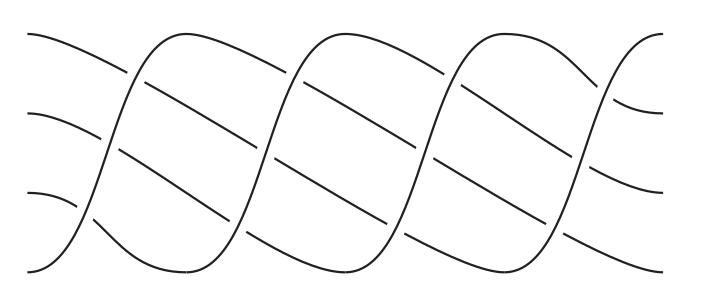
\includegraphics[width=6.5cm]{Images/volta_completa.png}
		\end{center}\caption{A volta completa, $\Delta_n^2$.}
		\label{full twist}
	\end{figure}
	
	\par\vspace{0.3cm} Da Figura \eqref{full twist}, podemos ver que $\Delta_n^2 = (\sigma_1\sigma_2\cdots\sigma_{n-1})^n$. Além disso, podemos também denotar por $\Delta_n$ a meia volta, e podemos escrevê-la em termos dos geradores $\sigma_i$ de $B_n$ da seguinte forma: $\Delta_n = (\sigma_1\sigma_2\cdots\sigma_{n-1})(\sigma_1\sigma_2\cdots\sigma_{n-2})\cdots(\sigma_2\sigma_1)\sigma_1$. Daí, como a notação sugere, $\Delta_n^2$ realmente é o quadrado de uma trança (e também a raiz $n$-ésima de uma trança, como podemos ver da Figura \eqref{full twist}).
	
	\par\vspace{0.3cm} Em particular, note que a meia volta não comuta, em geral, com os geradores de $B_n$, uma vez que $\Delta_n\sigma_2\neq\sigma_2\Delta_n$, por exemplo. De fato, o que ocorre é que $\sigma_i\Delta_n = \Delta_n\sigma_{n-i}$, ou seja, o cruzamento $\sigma_i$ "desliza" (é claro que se $n$ é par e $i=n/2$, então $\Delta_n$ comuta com $\sigma_i$).
	
	\begin{figure}[H]
		\label{delta5}
		\begin{center}	
			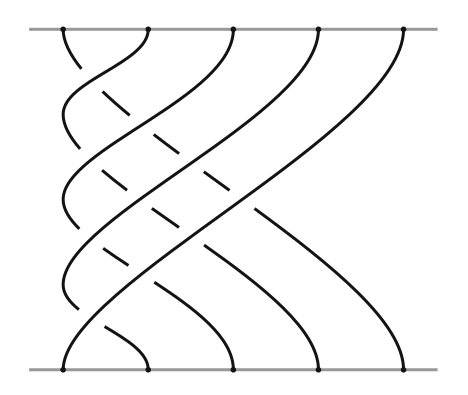
\includegraphics[width=6cm]{Images/delta5.png}
		\end{center}\caption{Diagrama de $\Delta_5$. Podemos ver que o cruzamento $\sigma_{i}$ "desliza", se tornando $\sigma_{n-i}$.}
	\end{figure}
	
	
	%\begin{center}
	%	\begin{tikzpicture}
	%	\label{delta}
	%	\braid[braid colour=black,strands=5,braid start={(0,0)}]	{\sigma_2\sigma_1 \sigma_2 \sigma_3\sigma_4\sigma_1\sigma_2\sigma_3\sigma_1\sigma_2\sigma_1}
	%	\node[font=\Huge] at (5.5,-5.5) {\(=\)};
	%	\braid[strands=5,braid start={(5,0)}]
	%	{\sigma_1 \sigma_2 \sigma_3\sigma_4\sigma_1\sigma_2\sigma_3\sigma_1\sigma_2\sigma_1\sigma_3}
	%	\end{tikzpicture}
	%\end{center}
	
	\par\vspace{0.3cm} Contudo, $\Delta_n^2$ comuta com toda trança de $B_n$, como é mostrado abaixo.
	
	\begin{proof}
		%Queremos mostrar que $\forall\beta\in B_n$, $\Delta_n^2\beta = \beta\Delta_n^2$. Isso equivale a mostrar que $\Delta_n^2\sigma_i = \sigma_i\Delta_n^2$. Por outro lado, como mostrado na Proposição \eqref{sigma1 e alfa geram B_n}, todo gerador de $B_n$ pode ser escrito em termos de $\sigma_1$ e $\alpha = \sigma_1\sigma_2\cdots\sigma_{n-1}$. Como $\alpha$ comuta com $\alpha^n = \Delta_n^2$, basta mostrarmos que $\sigma_1$ comuta com $\alpha^n$.
		
		
		
		Primeiro, note que $\sigma_i\Delta_n = \Delta_n\sigma_{n-i}$, como ilustram os diagramas acima. Daí, temos
		
		\begin{equation*}
		\sigma_i\Delta_n^2 = \sigma_i\Delta_n\Delta_n = \Delta_n\sigma_{n-i}\Delta_n = \Delta_n^2\sigma_i
		\end{equation*}
		
		\par\vspace{0.3cm} ou seja, $\Delta_n^2$ comuta com todo gerador de $B_n$ e, consequentemente, com toda trança de $B_n$.
		
		\par\vspace{0.3cm} 
		
	\end{proof}
	
	\par\vspace{0.3cm} Ora! Então $\Delta_n^2$ pertence ao centro de $B_n$. Na verdade, é possível mostrar que $\Delta_n^2$ gera o centro de $B_n$ para $n\geq 3$, i.e.
	
	
	\begin{theorem}
		\label{centro de B_n}
		Se $n\geq 3$, então $Z(B_n) = Z(P_n) = \langle \Delta_n^2 \rangle = \langle (\sigma_1\sigma_2\cdots\sigma_{n-1})^n \rangle$.
	\end{theorem}
	
	\par\vspace{0.3cm} Em outras palavras, toda trança do centro de $B_n$ é uma potência de $\Delta_n^2$.%, isto é, toda trança que comuta com todas as outras é uma potência da volta completa.
	
	\par\vspace{0.3cm} Demonstramos o Teorema \eqref{centro de B_n} para $n=3$.
	
	\begin{prop}
		$Z(B_3) = \langle (\sigma_1\sigma_2)^3 \rangle$
	\end{prop}
	
	\begin{proof}
		Primeiro, note que $(\sigma_1\sigma_2)^3\sigma_1 = \sigma_1\sigma_2\sigma_1\sigma_2\sigma_1\sigma_2\sigma_1 = \sigma_1(\sigma_1\sigma_2\sigma_1\sigma_2\sigma_1\sigma_2) = \sigma_1(\sigma_1\sigma_2)^3$ e também que $(\sigma_1\sigma_2)^3\sigma_2 = \sigma_1\sigma_2\sigma_1\sigma_2\sigma_1\sigma_2\sigma_2 = \sigma_2(\sigma_1\sigma_2\sigma_1\sigma_2\sigma_1\sigma_2) = \sigma_2(\sigma_1\sigma_2)^3$. Portanto, $\langle (\sigma_1\sigma_2)^3 \rangle\subseteq Z(B_3)$.
		
		\par\vspace{0.3cm} Agora, seja $g\in Z(B_3)$. Então, devemos ter, necessariamente, $g\sigma_1 = \sigma_1g$ e $g\sigma_2 = \sigma_2g$. Suponha, então, $g = \sigma_1^i\sigma_2^j$. Daí, temos
		
		\begin{align*}
		\begin{cases}
		\sigma_1^i\sigma_2^j\sigma_1 = \sigma_1^{i+1}\sigma_2^j \\
		\sigma_1^i\sigma_2^{j+1} = \sigma_2\sigma_1^{i}\sigma_2^j
		\end{cases} \Rightarrow \begin{cases}
		\sigma_2^j\sigma_1 = \sigma_1\sigma_2^j \\
		\sigma_1^i\sigma_2 = \sigma_2\sigma_1^i
		\end{cases} \Rightarrow i = j = 0 
		\end{align*} 
		
		\par\vspace{0.3cm} Suponha, agora, $g = (\sigma_1\sigma_2)^i$, $i\neq 0$. Então, temos
		
		\begin{align*}
		\begin{cases}
		(\sigma_1\sigma_2)^i\sigma_1 = \sigma_1(\sigma_1\sigma_2)^i \\
		(\sigma_1\sigma_2)^i\sigma_2 = \sigma_2(\sigma_1\sigma_2)^i
		\end{cases} \Rightarrow i = 3k, k\in\mathbb{Z}
		\end{align*}
		
		\par\vspace{0.3cm} A última implicação se deve ao seguinte raciocínio. A quantidade de termos no produto $(\sigma_1\sigma_2)^i\sigma_1$ é $2i+1$. Para transformar $(\sigma_1\sigma_2)^i\sigma_1$ em $\sigma_1(\sigma_1\sigma_2)^i$, devemos manipular os $2i$ termos de $\sigma_2(\sigma_1\sigma_2)^{i-1}\sigma_1$ usando a relação $\sigma_1\sigma_2\sigma_1 = \sigma_2\sigma_1\sigma_2$ para chegar em $(\sigma_1\sigma_2)^i$. Ora! Mas para utilizar a relação, precisamos de blocos de $3$ geradores, ou seja, devemos ter $i\in\mathbb{Z}$ tal que $\displaystyle{\frac{2i}{3}\in\mathbb{Z}}$. Como $2$ e $3$ são relativamente primos, devemos ter $i$ múltiplo de $3$.
		\par Por exemplo, $$\sigma_2(\sigma_1\sigma_2)^{4-1}\sigma_1 = \sigma_2\sigma_1\sigma_2\sigma_1\sigma_2\sigma_1\sigma_2\sigma_1 = \sigma_1\sigma_2\sigma_1\sigma_2\sigma_1\sigma_2\sigma_2\sigma_1 = (\sigma_1\sigma_2)^3\sigma_2\sigma_1\neq(\sigma_1\sigma_2)^4.$$
		
		\par\vspace{0.3cm} Daí, concluímos que todo elemento do centro de $B_3$ é uma potência de $(\sigma_1\sigma_2)^3$, ou seja, $Z(B_3)\subseteq\langle (\sigma_1\sigma_2)^3 \rangle$.
		
		\par\vspace{0.3cm} Portanto, $Z(B_3) = \langle (\sigma_1\sigma_2)^3 \rangle$.
		
	\end{proof}
	
	\begin{prop}
		Mostre que $l(\Delta_n^2) = n(n-1)$, sendo $l$ a função homomorfismo de comprimento definida no Lema \eqref{homomorfismo de comprimento} e $\Delta_n^2$ a volta completa em $B_n$.
	\end{prop}
	
	\begin{proof}
		Escrevendo $\Delta_n^2 = (\sigma_1\sigma_2\cdots\sigma_{n-1})^n$, segue da definição de $l$ que $l(\Delta_n^2) = n(n-1)$. 
		
		\par\vspace{0.3cm} Também podemos escrever $l(\Delta_n^2) = 2l(\Delta_n)$ e, como $\Delta_n = (\sigma_1\sigma_2\cdots\sigma_{n-1})(\sigma_1\sigma_2\cdots\sigma_{n-2})\cdots(\sigma_1\sigma_2)\sigma_1$, então $l(\Delta_n^2) = 2\Big( (n-1) + (n-2) + \cdots + 2 + 1 \Big) 2\Big( \displaystyle{\frac{n(n-1)}{2}} \Big) = n(n-1)$.
		
	\end{proof}
	
	%\begin{remark}
	%	No Teorema \eqref{centro de B_n}, usamos o fato de que $Z(B_n) = Z(P_n)$. Isso se deve ao fato de que $P_n$ é homomorfo a $B_n$, logo (como um homomorfismo preserva a operação) o centro de $B_n$ é levado no centro de $P_n$.
	%\end{remark}
	
	
	
	%\begin{theorem}
	%	$B_n$ e todos seus subgrupos são residualmente finitos.
	%\end{theorem}
	
	\par\vspace{0.3cm} Por fim, seja $f_n: P_n\to P_{n-1}$. Essa função é um homomorfismo sobrejetor, chamada \textit{homomorfismo esquecido}. A função $f_n$ pega uma trança em $P_n$, retira a $n$-ésima corda e a mapeia à trança resultante em $P_{n-1}$.
	\par\vspace{0.3cm} Para $n\geq 2$, definimos $U_n\vcentcolon=\Ker(f_n: P_n\to P_{n-1})$. Do diagrama do gerador de Artin, $A_{i,j}$, fica claro que $A_{i,n}\in U_n$, com $1\leq i\leq n-1$. 
	
	\begin{theorem}
		\label{U_n livre nos geradores de Artin}
		Para todo $n\geq 2$, $U_n$ é livre nos $n-1$ geradores $\{ A_{i,n} \}_{i=1,2,\dots,n-1}$.
	\end{theorem}
	
	\par\vspace{0.3cm} Aceitaremos o Teorema \eqref{U_n livre nos geradores de Artin} sem demonstração. Contudo, um corolário interessante é o seguinte.
	
	\begin{corollary}
		\label{B_n residualmente finito}
		$B_n$ e seus subgrupos são residualmente finitos.
	\end{corollary}
	
	\begin{proof}
		Um grupo $G$ é dito residualmente finito se para todo $\beta\in G-\{1\}$ existe um homomorfismo $f$ de $G$ em um grupo finito tal que $f(\beta)\neq 1$.
		\par\vspace{0.3cm} Sabemos que grupos livres são residualmente finitos e que o produto semidireto de dois grupos finitamente gerados e residualmente finitos é também residualmente finito.
		\par\vspace{0.3cm} Também sabemos, do Teorema \eqref{subgrupos normais e nucleos}, que $U_n\vartriangleleft P_n$. Da Definição \eqref{produto semidireto}, temos $P_n\cong U_n\rtimes P_{n-1}$. Tanto $U_n$ quanto $P_{n-1}$ são finitamente gerados e do Teorema \eqref{U_n livre nos geradores de Artin}, $U_n$ é residualmente finito. Daí, por indução em $n$, o Teorema \eqref{U_n livre nos geradores de Artin} implica $P_n$ residualmente finito.
		\par\vspace{0.3cm} Note que qualquer extensão de um grupo residualmente finito $P$ por um grupo finito é residualmente finita. Como $B_n$ é uma extensão de $P_n$ por $S_n$ e $P_n$ é residualmente finito, concluímos que $B_n$ também é.
		\par\vspace{0.3cm} Por fim, observe que todos os subgrupos de um grupo residualmente finito são também residualmente finitos.	
	\end{proof}
	\section{Tranças como espaços de configuração}\label{secao trancas como espacos de configuracao}
	\hspace{12pt} Há varias conexões entre grupos de tranças e topologia, e uma delas envolve \textit{espaços de configuração}, que nada mais são do que um espaço que contém todos os estados possíveis de um sistema. Por vezes, espaços de configuração são chamados de \textit{espaços de estado} ou \textit{espaços de parâmetros}.
	\par\vspace{0.3cm} Por exemplo, podemos usar um espaço de configuração para modelar o movimento coletivo de vários objetos, como carros nas ruas de uma cidade ou pacotes em uma \textit{network} ou moléculas em uma solução ou ainda robôs em uma fábrica.
	\par\vspace{0.3cm} Para um exemplo mais concreto, considere o seu braço. Nele, há três juntas: uma no ombro, uma no cotovelo e uma no pulso. Tanto o seu ombro quanto o seu pulso têm dois graus de liberdade (i.e., podem girar em dois sentidos diferentes), enquanto que o seu cotovelo tem apensa um grau de liberdade, totalizando cinco dimensões de configuração.
	\par\vspace{0.3cm} Um braço robótico modelado a partir do seu braço tem de navegar por um espaço de configuração cinco-dimensional para poder aproveitar toda a flexibilidade existente nesse sistema de juntas. Para ilustrar, imagine que ao invés de uma mão, você tem uma plataforma rígida conectada ao seu pulso e suponha que você queira levantar um copo d'água de abaixo da sua cintura até acima do seu ombro. Isso não será possível de fazer com a plataforma rígida no lugar da mão, porque apenas a rotação do ombro não é suficiente para fazer o movimento desejado (isso é o que os bebês fazem, e eles derramam a água sempre).
	\par\vspace{0.3cm} Mas qual a conexão entre espaços de configuração e grupos de trança? Bom, até agora, falamos de tranças individuais como objetos topológicos, como indicam as Definições \eqref{def geometrica tranca} e \eqref{outra def geometrica tranca}. Contudo, os grupos de trança em si também são objetos topológicos, no sentido de que cada grupo de trança descreve, de forma natural, os diferentes tipos de \textit{loops} que existem em um certo espaço de configuração. O espaço em questão modela o movimento coletivo de $n$ partículas distintas no plano que não podem colidir.
	\par\vspace{0.3cm} Então, imagine $n$ partículas no plano e estenda esse plano para formar a parede esquerda de uma trança. Agora, deslize o plano da esquerda para a direita, e imagine que cada partícula deixa um rastro à medida que o plano se move. O que acontece?
	\par\vspace{0.3cm} Bom, se as partículas ficam paradas (no plano), então quando o plano parar, você terá $n$ trilhas paralelas: a trança identidade! 
	
	
	\begin{figure}[H]
		\begin{center} 
			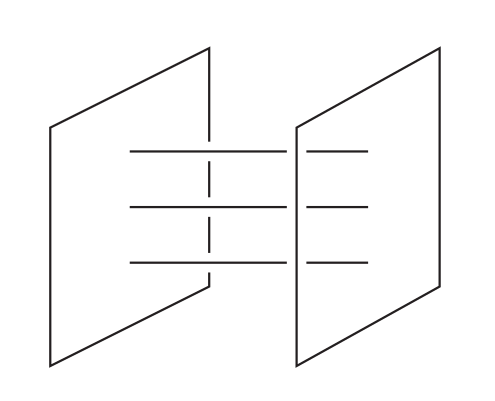
\includegraphics[width=9cm]{Images/tranca_identidade_conf.png}
		\end{center}\caption{A trança identidade em um espaço de configuração}\label{tranca identidade espaco configuracao}
	\end{figure}
	
	\par\vspace{0.3cm} Entretanto, se as partículas se movem no plano à medida que eles desliza, o que ocorre? Bom, desde que nenhum par de partículas colida, veremos uma trança! E claramente toda trança pode ser feita desse modo. Veja a figura abaixo. Note que estamos visualizando a direção $x$ como o eixo temporal.
	\par\vspace{0.3cm} Para um exemplo mais visual, podemos observar o movimento dos planetas do Sistema Solar, como nesse vídeo.\footnote{ \url{https://www.youtube.com/watch?v=0jHsq36_NTU&list=WL&index=2&t=50s}} 
	
	\begin{figure}[H]
		\begin{center}
			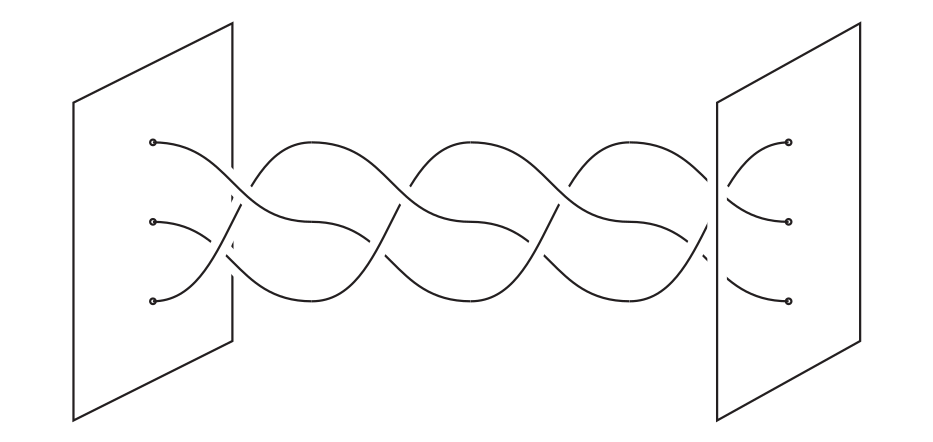
\includegraphics[width=10cm]{Images/tranca_conf.png}
		\end{center}\caption{Uma trança não trivial em um espaço de configuração.}\label{tranca espaco configuracao}
	\end{figure} 
	%\newpage
	\par\vspace{0.3cm} Para fazermos o produto de duas tranças usando essa ideia, precisamos ter certeza de que o coletivo de partículas no final da trança está no mesmo lugar que no começo da trança, pois assim podemos concatenar duas tranças sem haver nenhuma descontinuidade no meio.
	\par\vspace{0.3cm} A posição inicial é uma \textit{configuração} de $n$ partículas. O conjunto de todas as configurações possíveis é o espaço de configuração
	\begin{align}
	C_n(\mathbb{R}^2) = \{ (p_1, \dots, p_n)\in (\mathbb{R}^2)^n | p_i\neq p_j \text{ para }i\neq j \} 
	\label{configuracao ordenada}
	\end{align}
	\par\vspace{0.3cm} em que a condição $p_i\neq p_j$ indica a necessidade de um par partículas não colidirem.
	\par\vspace{0.3cm} O que definimos em \eqref{configuracao ordenada} foi o conjunto de configurações \textit{ordenadas}. Como o nosso propósito é descrever tranças, gostaríamos de ignorar a ordem e apenas focar no conjunto de partículas, e.g., queremos considerar $(p_1, p_2)$ como o mesmo que $(p_2, p_1)$ e pensar em ambos apenas como $\{p_1, p_2\}$. Para isso, definimos a versão não ordenada:
	\begin{align}
	UC_n(\mathbb{R}^2) = \{ \{ p_1, \dots, p_n\}\subset\mathbb{R}^2| p_i\neq p_j \text{ para }i\neq j  \}\label{configuracao nao ordenada}
	\end{align} 
	\par\vspace{0.3cm} ou, em palavras, o conjunto de subconjuntos de $n$ pontos do plano. 
	\par\vspace{0.3cm} Podemos também denotar $C_n(\mathbb{R}^2)$ por $\mathbb{F}_n(\mathbb{R}^2)$ e $UC_n(\mathbb{R}^2)$ por $\widetilde{\mathbb{F}}_n(\mathbb{R}^2)$, sendo $\sim$ a relação de equivalência cujas classes são os conjuntos de permutações de um dado ponto em $(\mathbb{R}^2)^n$. 
	\par\vspace{0.3cm} De forma geral, se $\mathbb{M}$ é uma variedade de dimensão maior ou igual a 2, então $\mathbb{F}_n(\mathbb{M})$ denota o subespaço de $\mathbb{M}^{(n)}$ definido por
	\begin{align}
	\mathbb{F}_n(\mathbb{M}) = \{ (x_1, \dots, x_n)\in \mathbb{M}^{(n)} | x_i\neq x_j \text{ para }i\neq j \} 
	\label{espaco de configuracao de M}
	\end{align}
	\par\vspace{0.3cm} Esse subespaço é chamado \textit{espaço de configuração} de $\mathbb{M}$. Sendo $\sim$ a mesma relação de equivalência definida acima, o espaço quociente $^{\displaystyle{\mathbb{F}_n(\mathbb{M})}}/_{\sim}$, que também pode ser denotado por $\widetilde{\mathbb{F}}_n(\mathbb{M})$, é definido por
	\begin{align}
	\widetilde{\mathbb{F}}_n(\mathbb{M}) = \{ \{ x_1, \dots, x_n\}\subset\mathbb{M}| x_i\neq x_j \text{ para }i\neq j  \}\label{espaco de configuracao nao ordenado de M}
	\end{align} 
	\par\vspace{0.3cm} Pelo modo como definimos $\sim$ acima, podemos ver que $UC_n(\mathbb{R}^2) = \displaystyle{C_n(\mathbb{R}^2)}/\displaystyle{S_n}$. Agora, voltando na Figura \eqref{tranca espaco configuracao}, tanto a parede da esquerda quando a parede da direita representam pontos de $UC_3(\mathbb{R}^2)$. Na verdade, as duas paredes representam o mesmo ponto (mas não o mesmo ponto de $C_3(\mathbb{R}^2)$, pois a configuração final é $(p_2, p_3, p_1)$, sendo $p_1$ o ponto inferior e $p_3$ o ponto superior). 
	\par\vspace{0.3cm} Além disso, quando deslizamos a parede da esquerda para a direita de forma a criar a trança, em cada instante de tempo temos um ponto de $UC_3(\mathbb{R}^2)$. Isso se deve ao fato de que cada corda é monotônica. Em outras palavras, podemos ver a trança como um \textit{loop} em $UC_3(\mathbb{R}^2)$.
	\par\vspace{0.3cm} Para fixar, podemos pensar em esquerda-direita como o eixo temporal, e então a trança tridimensional toda é como um filme de três partículas dançando no plano bidimensional (sem colidir) e retornando ao lugar onde começaram.
	\par\vspace{0.3cm} Equivalentemente, a trança é o gráfico de uma função $[0,1]\to UC_3(\mathbb{R}^2)$, cujos pontos inicial e final concordam. Ou seja, podemos pensar em tranças como \textit{loops} de configurações. De fato, essa é, essencialmente, uma correspondência injetiva.
	\par\vspace{0.3cm} Antes de prosseguir, definimos (informalmente) o conceito de grupo fundamental.
	
	\begin{deff}
		\label{def informal grupo fundamental}
		Dado um espaço topológico $X$ e um ponto $x_0\in X$, o conjunto de loops que começam e terminam em $x_0$ e que são caminhos fechados em $X$ é chamado grupo fundamental de $X$ com ponto base $x_0$ e denotado por $\pi_1(X,x_0)$.
	\end{deff}
	
	\par\vspace{0.3cm} Um detalhe importante é que se $X$ é conexo por caminhos (i.e., dado um par de pontos em $X$, existe um caminho totalmente contido em $X$ que liga esses dois pontos), então a escolha do ponto base não faz diferença. Esse é o nosso caso, e então denotaremos o grupo fundamental de $X$ por $\pi_1(X)$ apenas.
	\par\vspace{0.3cm} Com a Definição \eqref{def informal grupo fundamental}, podemos enunciar o seguinte teorema.
	
	\begin{theorem}
		\label{grupo fundamental de tranca}
		O grupo fundamental $\pi_1(UC_n(\mathbb{R}^2))$ é isomorfo ao grupo de trança $B_n$, e o grupo fundamental $\pi_1(C_n(\mathbb{R}^2))$ é isomorfo ao grupo de tranças puras $P_n$.
	\end{theorem} 
	
	\par\vspace{0.3cm} Da Definição \eqref{def informal grupo fundamental}, podemos ver que o grupo fundamental trata sobre os diferentes \textit{loops} em um espaço topológico. A noção de equivalência de \textit{loops} (i.e., homotopia, que nada mais é que uma deformação contínua de um caminho para outro) se traduz diretamente para nossa noção de equivalência de tranças.
	\par\vspace{0.3cm} Portanto, o Teorema \eqref{grupo fundamental de tranca} nos diz não só que tranças podem ser vistas como \textit{loops} em um espaço de configuração, mas também que podemos construir todos os \textit{loops} nesse espaço de configuração dessa maneira.
	\par\vspace{0.3cm} Além de nos proporcionar um outro modo de pensar em tranças, essa perspectiva topológica é útil tanto para provar coisas sobre tranças quanto para realizar generalizações interessantes. Por exemplo, é possível demonstrar o Teorema \eqref{apresentacao de B_n} usando essas ideias. 
	\par\vspace{0.3cm} Para outro exemplo, observe que a própria notação, $C_n(\mathbb{R}^2)$ sugere uma generalização óbvia, de substituir $\mathbb{R}^2$ por outros espaços topológicos, como superfícies, grafos ou variedades. Da mesma forma, o conjunto de (classes de equivalência de) \textit{loops} em um espaço de configuração de $n$ partículas em um espaço topológico $X$ é chamado de \textit{grupo de trança associado a $X$}.
	\par\vspace{0.3cm} Em símbolos, escrevemos $\pi_1(UC_n(X)) = B_n(X)$ e $\pi_1(C_n(X)) = P_n(X)$. Desse modo, os grupos usuais $B_n$ e $P_n$ são, na verdade, $B_n(\mathbb{R}^2)$ e $P_n(\mathbb{R}^2)$.
	\par\vspace{0.3cm} Por exemplo, sendo $X = \mathbb{R}$ e tomando $n=2$, temos que
	\begin{align*}
	UC_2(\mathbb{R}) = \big\{  \{p_1,p_2\}\subset\mathbb{R}|p_1\neq p_2  \big\} \\
	C_2(\mathbb{R}) = \big\{ (p_1,p_2)\in\mathbb{R}^2|p_1\neq p_2 \big\}
	\end{align*}
	\par\vspace{0.3cm} ou seja, os espaços de configuração não ordenado e ordenado, respectivamente, de dois pontos em uma reta. Não é difícil perceber que tanto $C_2(\mathbb{R})$ quanto $UC_2(\mathbb{R})$ possuem 3 componentes conexos e, em geral, $C_n(\mathbb{R})$ e $UC_n(\mathbb{R})$ possuem $n+1$ componentes conexos. Também podemos tomar $X = \mathbb{S}^1$, ou seja, uma circunferência. Nesse caso, $C_n(\mathbb{S}^1)$ e $UC_n(\mathbb{S}^1)$ têm $n$ componentes conexos.
	\par\vspace{0.3cm} Agora, vamos considerar $X = \mathbb{S}^2$, a esfera em $\mathbb{R}^3$. Nesse caso, $B_n(X) = B_n(\mathbb{S}^2)$ é chamado de \textit{grupo de tranças esféricas}. Uma primeira pergunta natural seria: qual a diferença entre tranças esféricas e "tranças planares"? Bom, podemos imaginar as paredes dos diagramas das tranças planares como sendo pequenos pedaços de esferas enormes, por exemplo, como mostra a figura \eqref{diagrama tranca esferica}abaixo (na verdade, essa ideia pode ser aplicada a tranças em qualquer superfície, não apenas na esfera).
	
	\begin{figure}[H]
		\begin{center}
			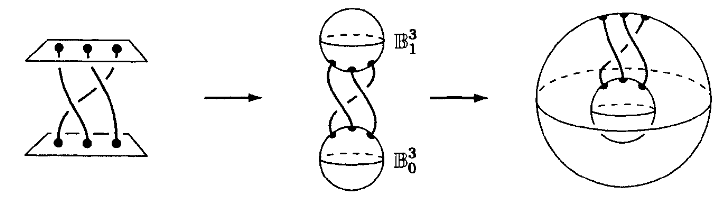
\includegraphics[width=12cm]{Images/diagrama_tranca_esferica.png}
		\end{center}\caption{Diagrama de uma trança esférica}
		\label{diagrama tranca esferica}
	\end{figure}
	\par\vspace{0.3cm} Logo, temos de modo natural a função $f: B_n(\mathbb{R}^2)\to B_n(\mathbb{S}^2)$. Não é muito difícil perceber que podemos obter toda trança esférica a partir de uma trança planar, i.e., que $f$ é sobrejetora. Contudo, $f$ não é injetora.
	\par\vspace{0.3cm} Isso se deve ao fato de que, para tranças esféricas, as cordas podem ser deformadas de modo a "darem a volta", como mostra a figura a seguir. Podemos pensar em $B_n(\mathbb{R}^2)$ como tranças dentro de um cubo, ficando "presas" lá dentro e, portanto, impossibilitadas de realizar movimentos como os que estão abaixo.
	
	\begin{figure}[H]
		\begin{center}
			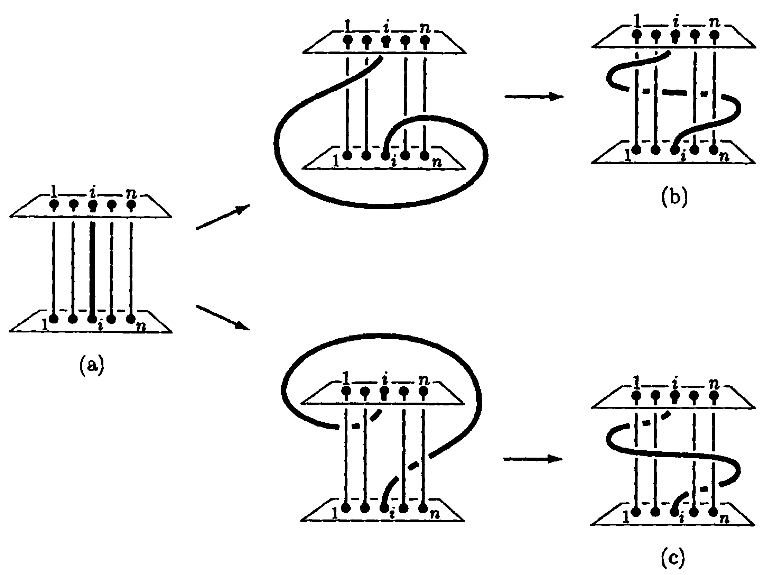
\includegraphics[width=10cm]{Images/movimentos_trancas_esfericas.png}
		\end{center}\caption{Movimentos possíveis para tranças esféricas, mas impossíveis para tranças planares}
		\label{movimentos trancas esfericas}
	\end{figure} 
	
	\par\vspace{0.3cm} Como os geradores $\sigma_i$ de $B_n(\mathbb{R}^2)$ também são geradores de $B_n(\mathbb{S}^2)$, as relações das tranças planares continuam válidas para as tranças esféricas. Contudo, os novos movimentos mostrados na Figura \eqref{movimentos trancas esfericas} nos dão uma nova relação em $B_n(\mathbb{S}^2)$, a saber
	\begin{align}
	\sigma_{i-1}\sigma_{i-2}\cdots\sigma_2\sigma_1^2\sigma_2\sigma_3\cdots\sigma_{n-2}\sigma_{n-1}^2\sigma_{n-2}\sigma_{n-3}\cdots\sigma_i = 1
	\label{novas relacoes}
	\end{align}
	\par\vspace{0.3cm} Contudo, toda relação, para $i=1,2\dots,n-1$, em \eqref{novas relacoes} é consequência da única relação
	\begin{align}
	(\sigma_1\sigma_2\cdots\sigma_{n-1})(\sigma_{n-1}\sigma_{n-2}\cdots\sigma_1) = 1
	\label{nova relacao}
	\end{align}
	\par\vspace{0.3cm} De fato, essa relação é dada pelo mesmo movimento que o diagrama (b) da Figura \eqref{movimentos trancas esfericas}, mas com a corda $1$ indo para a direita, como o diagrama abaixo.
	\begin{center}
		\begin{tikzpicture}
		\braid[braid colour=black,strands=4,braid start={(0,0)}]	{\sigma_1\sigma_2\sigma_3\sigma_3\sigma_2\sigma_1}
		%\node[font=\Huge] at (4.5,-1.0) {\(\neq\)};
		%\braid[strands=3,braid start={(5,0)}]
		%{\sigma_2\sigma_1}
		
		%gama em $B_4(\mathbb{S}^2)$
		\end{tikzpicture}
	\end{center}
	\par\vspace{0.3cm} Portanto, uma apresentação de $B_n(\mathbb{S}^2)$ tem os mesmos geradores e relações que $B_n(\mathbb{R}^2)$, mas com a última relação em \eqref{nova relacao}. De fato, essa é a apresentação completa de $B_n(\mathbb{S}^2)$, conforme o teorema abaixo, que não será demonstrado.
	
	\begin{theorem}
		\label{apresentacao de B_n(S^2)}
		O grupo de tranças esféricas $B_n(\mathbb{S}^2)$ tem apresentação	
		\begin{align*}
		B_n(\mathbb{S}^2) = \langle \sigma_1, \sigma_2, \dots, \sigma_{n-1}|&\sigma_i\sigma_j = \sigma_j\sigma_i, \text{ para } |i - j|>1, \\ 
		&\sigma_i\sigma_{i+1}\sigma_i = \sigma_{i+1}\sigma_i\sigma_{i+1}, \text{ para } 1\leq i\leq n-2 , \\
		&\sigma_1\sigma_2\cdots\sigma_{n-2}\sigma_{n-1}^2\sigma_{n-2}\cdots\sigma_2\sigma_1 = 1  \rangle.
		\end{align*} 
	\end{theorem}  
	
	\par\vspace{0.3cm} Então, voltando à nossa função $f$: ela não é injetora, pois a trança em \eqref{nova relacao} pertence ao núcleo de $f$, ou seja, $\Ker f$ não é trivial. Outra trança que pertence ao núcleo de $f$ é $\displaystyle{(\Delta_n^2)^2}$, o quadrado da volta completa, que tem ordem $2$ em $B_n(\mathbb{S}^2)$.
	\par\vspace{0.3cm} Na verdade, esse fato pode ser generalizado no seguinte lema.
	
	\begin{lemma}
		\label{potencia da volta completa trivial}
		Para todo $n> 2$, a trança de Dirac $\delta = (\sigma_1\sigma_2\cdots\sigma_{n-1})^{kn} = (\Delta_n^2)^k$ é trivial em $B_n(\mathbb{S}^2)$ se, e só se, $k$ é par. 
	\end{lemma}
	
	\begin{proof}
		Já sabemos que $(\Delta_n^2)^2 = 1$ em $B_n(\mathbb{S}^2)$. Então, se $k$ é par, podemos escrever $k=2j$ e segue que $(\Delta_n^2)^k = [(\Delta_n^2)^2]^j = 1^j = 1$. Por outro lado, como $|\Delta_n^2| = 2$ em $B_n(\mathbb{S}^2)$, então $(\Delta_n^2)^k = 1$ implica que $2|k$, i.e, $k$ par.
	\end{proof}
	\par\vspace{0.3cm} Do Teorema \eqref{apresentacao de B_n(S^2)}, podemos obter alguns fatos interessantes sobre o grupo de tranças esféricas. Por exemplo, $B_2(\mathbb{S}^2) = \langle \sigma_1|\sigma_1^2=1 \rangle$, ou seja, $B_2(\mathbb{S}^2)$ é um grupo finito de ordem $2$ com um gerador: $\mathbb{Z}_2$. Além disso, também podemos definir o homomorfismo de comprimento que definimos para as tranças planares, mas com uma pequena alteração.
	
	\begin{prop}
		\label{homomorfismo de comprimento em trancas esfericas}
		Seja $\beta\in B_n(\mathbb{S}^2)$. Tomando $\beta = \sigma_{i_1}^{\varepsilon_1}\cdots\sigma_{i_k}^{\varepsilon_k}$, sendo $\varepsilon_i = \pm1$ para $i=1,2,\dots,k$, então podemos definir a função $l$, chamada \textit{homomorfismo de comprimento}, de $B_n(\mathbb{S}^2)$ em $\mathbb{Z}$ como	
		\begin{align*}
		l(\beta) = \sum_{i=1}^{k}\varepsilon_i\text{ }\mathrm{mod}(2(n-1))
		\end{align*}
		\par\vspace{0.3cm} ou seja, a soma dos expoentes módulo $2(n-1)$. Então, $l$ é invariante em $B_n(\mathbb{S}^2)$, i.e., se $\beta = \beta'$ em $B_n(\mathbb{S}^2)$, então $l(\beta) = l(\beta')\text{ }\mathrm{mod}(2(n-1))$.
	\end{prop}
	
	\begin{proof}
		Do Teorema \eqref{apresentacao de B_n(S^2)}, sabemos todas as relações de $B_n(\mathbb{S}^2)$. Para as duas primeiras, $l(\beta)$ é constante para cada uma dessas relações. Contudo, para a terceira relação, $l(\beta)$ difere por um fator de $\pm2(n-1)$ para os dois lados da relação. Como $l(1) = 0$ e $l$ está bem definida (demonstração análoga à do Lema \eqref{homomorfismo de comprimento}), devemos ter a igualdade módulo $2(n-1)$.
	\end{proof}
	
	\par\vspace{0.3cm} Por exemplo, como $l((\sigma_1\sigma_2)^3) = 6\neq 0\text{ }\mathrm{mod}4$ e $l(1) = 0$, então, em $B_3(\mathbb{S}^2)$, $(\sigma_1\sigma_2)^3\neq 1$. Outro exemplo: $\sigma_1^4=1$ em $B_3(\mathbb{S}^2)$, mas $\sigma_1^4\neq1$ em $B_4(\mathbb{S}^2)$. Esse exemplo nos mostra uma diferença notável entre $B_n(\mathbb{R}^2)$ e $B_n(\mathbb{S}^2)$, pois se $\beta$ é trivial em $B_m(\mathbb{R}^2)$ e $m\leq n$, então $\beta$ também é trivial em $B_n(\mathbb{R}^2)$, enquanto que para $B_m(\mathbb{S}^2)$ e $B_n(\mathbb{S}^2)$ isso, em geral, não é verdade.
	\par\vspace{0.3cm} Note também que a recíproca da Proposição \eqref{homomorfismo de comprimento em trancas esfericas} é falsa. Por exemplo, $\sigma_1^6\neq1$ em $B_4(\mathbb{S}^2)$ mas $l((\sigma_1)^6) = 0\text{ }\mathrm{mod}6 = l(1)$.
	\par\vspace{0.3cm} A apresentação no Teorema \eqref{apresentacao de B_n(S^2)} tem também uma interessante consequência, enunciada no Lema \eqref{B_3(S^2) tem ordem 12}. Antes, contudo, introduziremos um pequeno conceito, as \textit{transformações de Tietze}.
	\subsubsection{Transformações de Tietze}
	\hspace{12pt} Dada uma apresentação de um grupo $G$, temos os seguintes movimentos:
	\begin{enumerate}
		\item se uma relação pode ser deduzida a partir das relações existentes, então podemos adicionar essa nova relação à apresentação. Por exemplo, se $G = \langle x|x^3=1 \rangle$, obtemos a relação $x^6 = 1$ a partir de $x^3=1$. Logo, podemos escrever $G = \langle x|x^3=1,x^6=1 \rangle$.
		\item Reciprocamente, se uma relação da apresentação pode ser deduzida a partir das outras, então podemos removê-la. Em $G = \langle x|x^3=1,x^6=1 \rangle$, a relação $x^6=1$ pode ser deduzida de $x^3=1$ e, portanto, pode ser removida da apresentação. Contudo, note que não podemos remover $x^3=1$, pois teríamos outro grupo.
		\item Podemos adicionar um gerador escrito como uma palavra nos geradores originais. Começando com $G = \langle x|x^3=1 \rangle$ e fazendo $y=x^2$, a nova apresentação $G = \langle x,y|x^3=1,y=x^2 \rangle$ define o mesmo grupo.
		\item De modo semelhante, se podemos formar uma relação em que um dos geradores é uma palavra nos outros geradores, então esse gerador pode ser removido. Por exemplo, a apresentação do grupo abeliano de ordem $4$, $G = \langle x,y,z|x=yz, y^2=1, z^2=1, x=x^{-1} \rangle$ pode ser substituído por $G = \langle y,z|y^2=1,z^2=1,(yz)=(yz)^{-1} \rangle$.
	\end{enumerate}
	
	\par\vspace{0.3cm} Usaremos essas transformações para demonstrar o seguinte lema.
	
	\begin{lemma}
		\label{B_3(S^2) tem ordem 12}
		$B_3(\mathbb{S}^2)$ tem apresentação $\langle a,b|b^6=1,a^2=b^3=(ab)^2 \rangle$, sendo, portanto, isomorfo a $Q_6$, o grupo dicíclico de ordem $12$. 
	\end{lemma} 
	
	\begin{proof}
		Sabemos, do Teorema \eqref{apresentacao de B_n(S^2)}, que $B_3(\mathbb{S}^2) = \langle \sigma_1,\sigma_2 | \sigma_1\sigma_2\sigma_1 = \sigma_2\sigma_1\sigma_2\text{, } \sigma_1\sigma_2^2\sigma_1 = 1\rangle$. Fazendo $a = \sigma_1\sigma_2\sigma_1$ e $b = \sigma_1\sigma_2$, temos:
		
		\begin{align*}
		a^2 = \sigma_1\sigma_2\sigma_1\sigma_1\sigma_2\sigma_1 = \sigma_1\sigma_2\sigma_1\sigma_2\sigma_1\sigma_2 = (\sigma_1\sigma_2)^3 = b^3 \\
		(ab)^2 = \sigma_1\sigma_2\sigma_1\sigma_1\sigma_2\sigma_1\sigma_2\sigma_1\sigma_1\sigma_2 =  \sigma_1\sigma_2\sigma_1\sigma_2\underbrace{\sigma_1\sigma_2\sigma_2\sigma_1}_{1}\sigma_1\sigma_2 = (\sigma_1\sigma_2)^3 = b^3 \\
		b^6 = \sigma_1\sigma_2\sigma_1\sigma_2\sigma_1\sigma_2\sigma_1\sigma_2\sigma_1\sigma_2 = \underbrace{\sigma_1\sigma_2\sigma_2\sigma_1}_{1}\sigma_2\sigma_2\underbrace{\sigma_1\sigma_2\sigma_2\sigma_1}_{1}\sigma_2\sigma_2 = \sigma_2^4 
		\end{align*}
		
		\par\vspace{0.3cm} Vamos mostrar que tanto $\sigma_1$ quanto $\sigma_2$ têm ordem 4. Então, seja $N$ o fecho normal de $a^2$, i.e., $N = \{1,a\}$. Daí, $N\vartriangleleft B_3(\mathbb{S}^2)$ e, portanto, o grupo quociente $B_3(\mathbb{S}^2)/N$ tem apresentação $\langle a,b|a^2=b^3=(ab)^2=1 \rangle$, que é a apresentação de $S_3$, o grupo simétrico em $3$ elementos. Logo, $|B_3(\mathbb{S}^2)| = |N||S_3| = 12$.
		\par\vspace{0.3cm} Por fim, note que $(ab)^2 = a^2$ implica $a = b^{-1}ab^{-1}$, logo
		\begin{align*}
		\sigma_1^4 = (b^{-1}a)^4 = (b^{-1}ab^{-1})a(b^{-1}ab^{-1})a = a^4 = 1\text{ (observe o diagrama abaixo)}
		\end{align*}  
		
		\begin{figure}[H]
			\begin{center}
				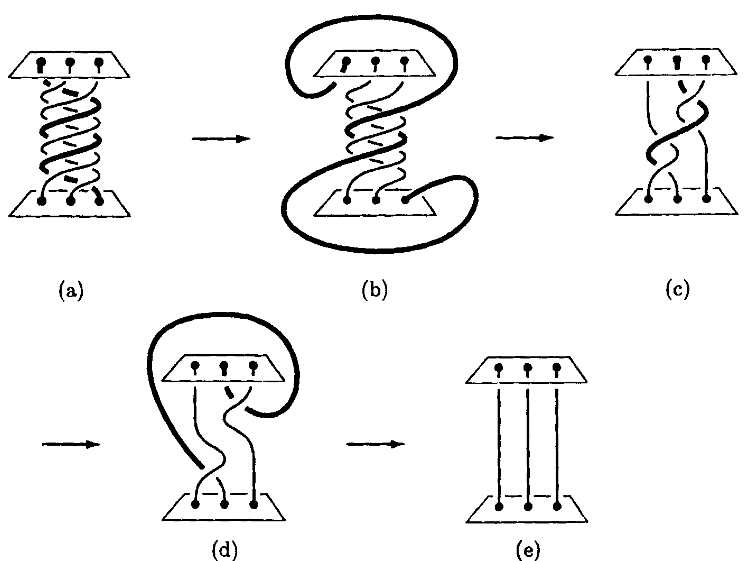
\includegraphics[width=12cm]{Images/manipulacao_de_a4.png}
			\end{center}\caption{$a^4 = 1$ em $B_3(\mathbb{S}^2)$}
		\end{figure}
		
		\par\vspace{0.3cm} Como $\sigma_1\neq 1$ e $\sigma_1^2\neq 1$, então, pela Proposição \eqref{homomorfismo de comprimento em trancas esfericas}, $|\sigma_1| = 4$.
		\par\vspace{0.3cm} Similarmente, $(ab)^2 = a^2$ implica $bab=a$ e também $ba=a^{-1}b^2$, logo
		\begin{align*}
		\sigma_2^4 = (a^{-1}b^2)^4 = (ba)^4 = (bab)a(bab)a = a^4 = 1
		\end{align*}
		\par\vspace{0.3cm} Como $\sigma_2\neq1$ e $\sigma_2^2\neq1$ então, da Proposição \eqref{homomorfismo de comprimento em trancas esfericas}, temos $|\sigma_2|=4$. 
		\par\vspace{0.3cm} Além disso, como $a^4 = 1$, temos $b^6=1$.
		\par\vspace{0.3cm} Por fim, da tabela \eqref{tabela grupos}, vemos que $B_3(\mathbb{S}^2)\cong Q_6$, o grupo dicíclico de ordem 12.
	\end{proof}
	
	\par\vspace{0.3cm} Do Lema \eqref{B_3(S^2) tem ordem 12}, podemos listar os elementos de $B_3(\mathbb{S}^2)$:
	\begin{align*}
	B_3(\mathbb{S}^2) = \left\{ 1, a, a^2, a^3, b, b^2, b^4, b^5, ab, ab^2, ab^4, ab^5 \right\}
	\end{align*}
	\par\vspace{0.3cm} Podemos ainda escrever esse elementos em termos dos geradores $\sigma_1$ e $\sigma_2$. Com algumas simplificações, obtemos:
	\begin{align*}
	B_3(\mathbb{S}^2) = \left\{ 1, \sigma_1\sigma_2\sigma_1, (\sigma_1\sigma_2\sigma_1)^2, (\sigma_1\sigma_2\sigma_1)^3, \sigma_1\sigma_2, (\sigma_1\sigma_2)^2, \sigma_1^3\sigma_2, \sigma_2\sigma_1, \sigma_1, \sigma_2^3, \sigma_2\sigma_1^3\sigma_2, \sigma_1^3 \right\}
	\end{align*}
	\par\vspace{0.3cm} Fazendo os diagramas, vemos que apenas $1$ e $(\sigma_1\sigma_2\sigma_1)^2 = a^2 = b^3$ são tranças puras. Além disso, como $a^4 = 1 = b^6$, concluímos que $P_3(\mathbb{S}^2) = \langle a^2 \rangle = \langle b^3 \rangle$.
	
	\par\vspace{0.3cm} Agora, vamos considerar $B_4(\mathbb{S}^2)$, que tem apresentação
	\begin{align*}
	B_4(\mathbb{S}^2) = \langle \sigma_1, \sigma_2, \sigma_3| &\sigma_1\sigma_2\sigma_1 = \sigma_2\sigma_1\sigma_2 \\ &\sigma_2\sigma_3\sigma_2 = \sigma_3\sigma_2\sigma_3 \\
	&\sigma_1\sigma_3 = \sigma_3\sigma_1\\
	&\sigma_1\sigma_2\sigma_3^2\sigma_2\sigma_1 = 1\rangle
	\end{align*}
	
	\par\vspace{0.3cm} Seja $N$ o fecho normal de $\sigma_1\sigma_3^{-1}$. Então, a apresentação do grupo quociente $G = B_4(\mathbb{S}^2)/N$, é obtida de $B_4(\mathbb{S}^2)$ adicionando a relação $\sigma_1\sigma_3^{-1} = 1$ ou, equivalentemente, $\sigma_1=\sigma_3$. O efeito dessa relação extra é reduzir o número de relações para duas, a saber
	\begin{center}
		\begin{tabular}{ccc}
			$\sigma_1\sigma_2\sigma_1 = \sigma_2\sigma_1\sigma_2$ & e & $\sigma_1\sigma_2\sigma_1^2\sigma_2\sigma_1 = 1$ \\
		\end{tabular}
	\end{center}
	
	\par\vspace{0.3cm} A última relação pode ser manipulada como a seguir:
	\begin{align*}
	1 &= \sigma_1\sigma_2\sigma_1\sigma_1\sigma_2\sigma_1 \\
	&= \sigma_1\sigma_2\sigma_1\sigma_2\sigma_1\sigma_2 \\ 
	&= (\sigma_1\sigma_2)^3  
	\end{align*}
	\par\vspace{0.3cm} Portanto, $G = \langle \sigma_1, \sigma_2| \sigma_1\sigma_2\sigma_1=\sigma_2\sigma_1\sigma_2\text{, } (\sigma_1\sigma_2)^3=1 \rangle$. Como antes, tome $a = \sigma_1\sigma_2\sigma_1$ e $b = \sigma_1\sigma_2$. Como $\sigma_1 = b^{-1}a$ e $\sigma_2 = a^{-1}b^2$, as relações de $G$ se tornam $a^2 = b^3$ e $b^3 = 1$, logo $G = \langle a,b|a^2=b^3=1 \rangle$. Vamos mostrar que $G$ é infinito, usando o seguinte lema, que será aceito sem demonstração.
	
	\begin{lemma}
		\label{grupo triangular}
		O grupo triangular, ou grupo de Dyck, $T(l,m,n) = \langle a,b|a^l=b^m=(ab)^n=1 \rangle$ é finito se, e só se, $\displaystyle{\frac{1}{l} + \frac{1}{m} + \frac{1}{n} - 1 > 0}$.
	\end{lemma}
	
	
	\begin{prop}
		\label{quociente de B4(S2) infinito}
		$G = \langle a,b|a^2=b^3=1 \rangle$ é infinito e, consequentemente, $B_4(\mathbb{S}^2)$ é infinito.
	\end{prop}
	
	\begin{proof}
		Seja $\widehat{G} = \langle a,b|a^2=b^3=(ab)^7=1 \rangle$. Note que $\widehat{G}$ é um grupo quociente de $G$ e, além disso, $\widehat{G} = T(2,3,7)$. Do Lema \eqref{grupo triangular}, temos $\widehat{G}$ infinito, pois $\displaystyle{\frac{1}{2} + \frac{1}{3} + \frac{1}{7} - 1 < 0}$. Logo, como $\widehat{G}$ é um grupo quociente de $G$, então $G$ também é infinito, pois se todo grupo finito com apresentação finita tem, no máximo, tantos geradores quanto relações. Por fim, como $G$ é um grupo quociente de $B_4(\mathbb{S}^2)$, temos $B_4(\mathbb{S}^2)$ infinito, também pelo mesmo fato citado acima sobre grupos finitos e finitamente apresentados. Observe que o número $7$ não tem nada de especial: poderíamos tomar qualquer $k\geq 7$.
	\end{proof}
	
	\par\vspace{0.3cm} Podemos, ainda, generalizar esse fato no seguinte lema, que não será demonstrado.
	
	\begin{lemma}
		\label{grupo de trancas esfericas infinitos}
		$|B_n(\mathbb{S}^2)| = \infty$ para todo $n\geq 4$.
	\end{lemma}
	
	\par\vspace{0.3cm} Observando o Lema \eqref{grupo de trancas esfericas infinitos}, a distinção mais simples que podemos fazer entre $B_n(\mathbb{R}^2)$ e $B_n(\mathbb{S}^2)$ é que $B_n(\mathbb{R}^2)$ é finito apenas para $n=1$, enquanto que $B_n(\mathbb{S}^2)$ é finito para $n=1,2$ e $3$.
	\par\vspace{0.3cm} Contudo, a maior diferença entre esses dois grupos (ou famílias de grupos) é o fato de que $B_n(\mathbb{R}^2)<B_{n+1}(\mathbb{R}^2)$, como mostrado na Proposição \eqref{B_m subgrupo de B_n}, enquanto que $B_n(\mathbb{S}^2)\nless B_{n+1}(\mathbb{S}^2)$.
	\par\vspace{0.3cm} De fato, a relação $(\sigma_1\sigma_2\cdots\sigma_{n-1})(\sigma_{n-1}\cdots\sigma_2\sigma_1) = 1$ em $B_n(\mathbb{S}^2)$ pode não ser válida em $B_{n+1}(\mathbb{S}^2)$. Por exemplo, do Teorema \eqref{apresentacao de B_n(S^2)}, sabemos que $\sigma_1^2 = 1$ em $B_2(\mathbb{S}^2)$, mas não em $B_3(\mathbb{S}^2)$, devido à Proposição \eqref{homomorfismo de comprimento em trancas esfericas}.
	\par\vspace{0.3cm} Além disso, também do Teorema \eqref{apresentacao de B_n(S^2)}, $\sigma_1\sigma_2^2\sigma_1 = 1$ em $B_3(\mathbb{S}^2)$, mas não em $B_4(\mathbb{S}^2)$, de novo devido à Proposição \eqref{homomorfismo de comprimento em trancas esfericas}.
	\par\vspace{0.3cm} Consequentemente, a função identidade $\displaystyle{\psi: \underset{\sigma_i\mapsto\sigma_i}{B_n(\mathbb{S}^2)\to B_{n+1}(\mathbb{S}^2)}}$, para $1\leq i\leq n-1$, não é um homomorfismo e não podemos considerar $B_n(\mathbb{S}^2)$ como um subgrupo natural de $B_{n+1}(\mathbb{S}^2)$.
	\par\vspace{0.3cm} É interessante notar também que algumas tranças não identidades são triviais em $B_n(\mathbb{S}^2)$, i.e., $B_n(\mathbb{S}^2)$ \textbf{não é} livre de torção, como mostrado no seguinte lema.
	
	\begin{lemma}
		\label{B_(S^2) nao livre de torcao}
		Para todo $n\geq2$, $\gamma = \sigma_1\sigma_2\cdots\sigma_{n-1}$ (a raiz $n$-ésima da volta completa) tem ordem finita maior que $1$ e, portanto, $B_n(\mathbb{S}^2)$ tem elementos de torção.
	\end{lemma}
	
	\begin{proof}
		Primeiro, note que como $l(\gamma) = (n-1)\neq0\text{ }\mathrm{mod}(2(n-1))$, então, para todo $n\geq2$, $\gamma\neq1$. Por outro lado, sabemos que o quadrado da volta completa é trivial, i.e., $(\Delta_n^2)^2 = 1$, logo, como $\Delta_n^2 = \gamma^n$, temos $\gamma^{2n} = 1$.
		\par\vspace{0.3cm} Portanto, $\gamma$ tem ordem finita $k$ com $2\leq k\leq 2n$, para todo $n\geq 2$. Consequentemente, $B_n(\mathbb{S}^2)$ tem elemento não trivial de ordem finita, não sendo, portanto, livre de torção.
	\end{proof}
	
	\section{Diagrama de van Kampen}
	\hspace{12pt} Vamos nos deter brevemente para descrever o \textbf{diagrama de van Kampen}. Inicialmente, podemos descrever o diagrama de van Kampen de modo visual: ele ilustra o fato de que uma palavra $w\in F(X)$ no grupo livre sobre $X$ é uma relação em um grupo $G$, i.e., $w$ é um produto de palavras em $R\cup R^{-1}$. Em um nível mais rigoroso, os diagrama de van Kampen são a base de um dos métodos mais poderosos da Teoria Combinatória dos Grupos.
	\par\vspace{0.3cm} Informalmente, o diagrama de van Kampen para uma apresentação $G = \langle X|R \rangle$ é um grafo conexo finito planar $\Gamma\subseteq\mathbb{R}^2$, cujas arestas são direcionadas e marcadas por elementos de $X$ em um caminho tal que toda face de $\Gamma$ é um disco cuja fronteira é marcada e pertence a $R$ (ou seja, é uma relação). Daí, é quase imediato que a palavra marcada sobre o bordo de $\Gamma$ é ela própria uma relação em $G$. Assim, o diagrama de van Kampen pode ser utilizado para ilustrar a dedução de novas relações a partir das antigas relações.
	\par\vspace{0.3cm} Antes dos exemplos, vejamos como que cada relator de $G$ é uma palavra limitando algum diagrama de van Kampen $\Gamma$ de $G$. Podemos, ainda, assumir que $\Gamma$ está reduzido, no sentido de que nenhum circuito não trivial carrega a palavra vazia. Agora, o fato de que $\Gamma$ está imerso no plano impõe severas restrições sobre sua estrutura, e.g., sobre a característica de Euler. Essas restrições podem ser usadas para argumentar sobre propriedades locais de $\Gamma$ (correspondendo a condições combinatoriais no conjunto $R$) e sobre propriedades do bordo (correspondendo a propriedades grupo teóricas de $G$).
	\par\vspace{0.3cm} Um modo de construir o diagrama de van Kampen para uma apresentação $G = \langle X|R \rangle$ é o seguinte. Pensemos em cada relator como o bordo de uma célula bidimensional. Podemos, então, colar coleções dessas células ao longo de arestas com a mesma palavra e orientação.
	\par\vspace{0.3cm} Por exemplo, o grupo dos quatérnios, $Q_8$, tem ordem $8$ e apresentação:
		\begin{equation*}
		\langle x,y \ | \ x^4=1, x^2=y^2, y^{-1}xy = x^{-1} \rangle
		\end{equation*}
		\par\vspace{0.3cm} Vamos fazer $r = x^4$, $s = x^2y^{-2}$ e $t = y^{-1}xyx$. Daí, o diagrama de van Kampen é o seguinte.
		\begin{figure}[H]
			\begin{center}
				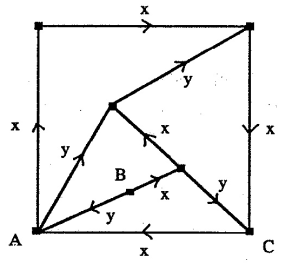
\includegraphics[width=5cm]{Images/diagrama_quaternios.png}
			\end{center}
		\caption{Diagrama de van Kampen para o grupo dos quatérnios, $Q_8$}
		\label{figura diagrama quaternios}
		\end{figure}
	\par\vspace{0.3cm} Na parte superior da face esquerda, a fronteira, lida no sentido horário a partir de $A$ é $s = x^2y^{-2}$. De modo análogo, a face contendo $B$, lida no sentido anti-horário a partir de $B$ também nos dá $s = x^2y^{-2}$. Na face inferior contendo $B$, a delimitação do bordo lida no sentido horário a partir de $A$ nos dá $t = y^{-1}xyx$. Do mesmo modo, a face mais à direita, lida no sentido horário a partir de $C$ também nos dá $t = y^{-1}xyx$. Por fim, como a marca sobre a fronteira, lida no sentido horário a partir de $A$, é $x^4=1$, isso nos mostra que essa primeira relação na apresentação de $Q_8$ é supérflua.	
	\par\vspace{0.3cm} Outro exemplo é o grupo 
		\begin{equation*}
		G = \langle a,b,c,d \ | \ ab = c, bc = d, cd = a, da = b \rangle
		\end{equation*}
		\par\vspace{0.3cm} é claramente gerado por $a$ e $b$, uma vez que $c = ab$ e $d = bc = bab$. Contudo, esse fato pode ser verificado a partir do diagrama de van Kampen para essa apresentação. Nele, as faces estão marcadas pelas seguintes relações definidoras:
		\begin{equation*}
		r_1 = abc^{-1}, \ r_2 = bcd^{-1}, \ r_3 = cda^{-1}, \ r_4 = dab^{-1}
		\end{equation*}
		\begin{figure}[H]
			\begin{center}
				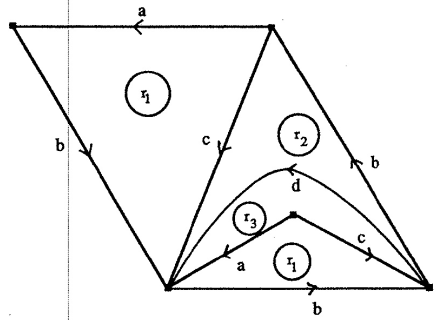
\includegraphics[width=7.5cm]{Images/diagrama_ciclico.png}
			\end{center}
		\caption{Diagrama de van Kampen de $G$}
		\label{figura diagrama ciclico}
		\end{figure}
		\par\vspace{0.3cm} A partir do diagrama, vemos que lendo a fronteira, no sentido anti-horário, a partir do vértice superior direito, temos $ab^3 = 1$, ou seja, $a = b^{-3}$ e, portanto, $G$ é gerado apenas por $b$, sendo cíclico. De fato, podemos fazer uma manipulação desse diagrama para obter o seguinte diagrama:
		\begin{figure}[H]
			\begin{center}
				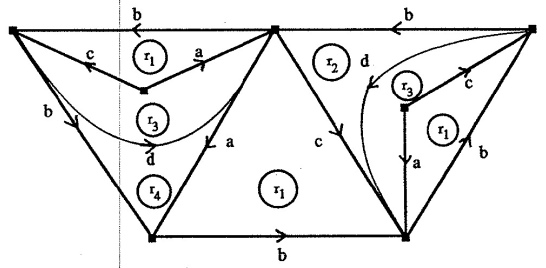
\includegraphics[width=7.5cm]{Images/diagrama_ciclico_2.png}
			\end{center}
		\caption{Diagrama de van Kampen manipulado de $G$}
		\label{figura diagrama ciclico 2}
		\end{figure}
	\par\vspace{0.3cm} A partir desse diagrama, vemos, a partir da leitura do bordo, que $b^5=1$. Logo, $G$ é o grupo cíclico de ordem $5$ ($b$ não trivial) ou $1$ ($b$ trivial).
	\par\vspace{0.3cm} É interessante notar que se $a$, $b$, $c$ e $d$ são geradores de um grupo tais que $a$ e $b$ comutam com $c$ e $d$, então o fato de que $ab$ comuta com $cd$ pode ser deduzido pelo seguinte diagrama:
		\begin{figure}[H]
			\begin{center}
				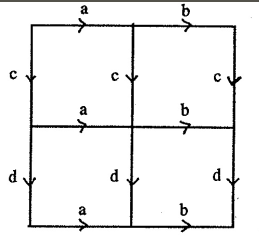
\includegraphics[width=5cm]{Images/diagrama_comutatividade.png}
			\end{center}
		\caption{Diagrama de van Kampen em que $a$ e $b$ comutam com $c$ e $d$}
		\label{figura diagrama comutatividade}
		\end{figure}
	\par\vspace{0.3cm} Do diagrama, é imediato que $abcd(ab)^{-1}(cd)^{-1} = 1$, ou seja, $[ab,cd] = 1$.	
	\par\vspace{0.3cm} Um último exemplo é o seguinte: fazendo $r = x^2yxy^3 = 1 = y^2xyx^3 = s$, obtemos o seguinte diagrama:
		\begin{figure}[H]
			\begin{center}
				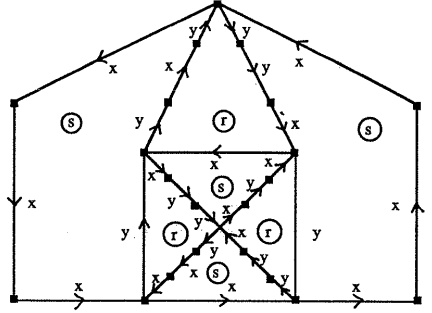
\includegraphics[width=7.5cm]{Images/diagrama_complicado.png}
			\end{center}
		\end{figure}
		\par\vspace{0.3cm} Da leitura do bordo no sentido anti-horário, obtemos $x^7=1$.
	\par\vspace{0.3cm} Dos exemplos acima, podemos ver que os diagramas de van Kampen nos ajudam a deduzir relações que não são tão imediatas tendo apenas a apresentação do grupo.
	
	\section{Tranças como discos perfurados}\label{secao trancas como discos perfurados}
	\hspace{12pt} Podemos, ainda, pensar em tranças de uma terceira maneira. Voltando na trança da Figura \eqref{tranca espaco configuracao}, vamos imaginar o seguinte: suponha que a trança é feita de fios rígidos, e que o plano é, na verdade, uma seção quadrada do plano (como está desenhado), ou seja, um disco topológico, exceto que esse disco tem buracos.
	\par\vspace{0.3cm} Agora, imagine que o interior do disco é feito de um material muito flexível e que a fronteira (bordo) quadrada é uma armação rígida (parecida com aqueles \textit{frisbees} de tecido, apenas quadrados). Imagine o processo de empurrar esse disco perfurado ao longo da trança de fios rígidos até chegar na parede da direita. A trança não se moveu, mas o disco em si foi todo torcido, ou seja, a trança provocou uma mudança na superfície.
	\par\vspace{0.3cm} Mais especificamente, o que aconteceu ao disco perfurado foi que a trança implementou um homeomorfismo da superfície nela mesma. O bordo fica fixo, porque é rígido, e as perfurações são permutadas conforme a permutação associada à trança. Funções como essa, a menos de homotopia, formam o \textit{grupo de classes} de $D_n$, um disco com $n$ perfurações com bordo $\partial D_n$ (e não o grupo diedral):
	\begin{align*}
	\Mod(D_n) = \{ f:D_n\to D_n|& f\text{ é homeomorfismo}, \\
	&f|_{\partial D_n} = 1 \}/\text{Homotopia}
	\end{align*}
	
	\begin{figure}[H]
		\begin{center}
			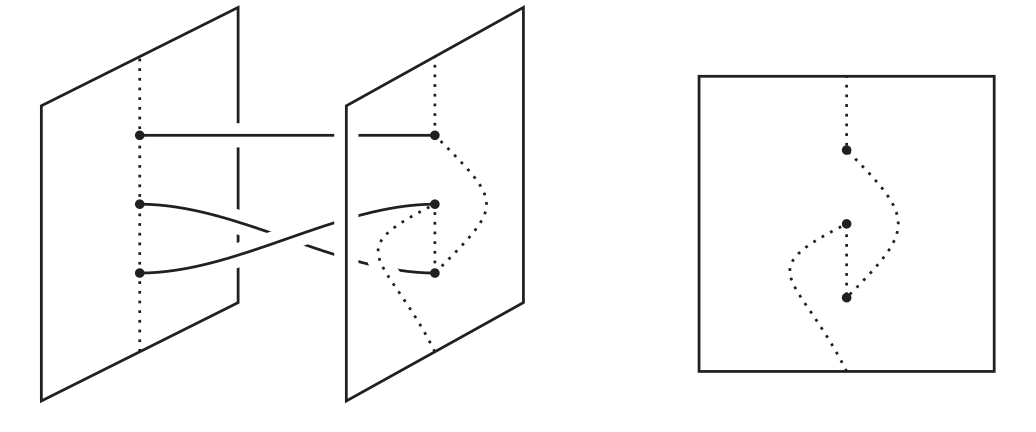
\includegraphics[width=10cm]{Images/tranca_disco_perfurado.png}
		\end{center}\caption{Diagrama de curva associado a $\sigma_1$.}
		\label{tranca disco perfurado}
	\end{figure}
	
	\par\vspace{0.3cm} A operação do grupo é a composição de funções: dois homeomorfismos $f$ e $g$ podem ser compostos para formar um homeomorfismo $g\circ f$ (ou $f\circ g$, que geralmente é diferente). Acima, descrevemos uma função $\psi: B_n\to\Mod(D_n)$, a saber, dada uma trança, deslize o disco pela trança e considere o homeomorfismo resultante. De fato, $\psi$ é, na verdade, um isomorfismo.
	
	\begin{theorem}
		\label{B_n isomorfo a Mod(D_n)}
		$B_n\cong \Mod(D_n)$ 
	\end{theorem}
	
	\begin{proof}
		Não demonstraremos a sobrejetividade de $\psi$, pois exige conhecimentos além do escopo deste relatório.
		\par\vspace{0.3cm} Primeiro, note que $\psi$ está bem definida, pois se $\alpha, \beta\in B_n$ são tais que $\alpha = \beta$, então elas induzem a mesma deformação no disco, i.e., o mesmo homeomorfismo e, portanto, temos $\psi(\alpha) = \psi(\beta)$.
		\par\vspace{0.3cm} Além disso, o núcleo de $\psi$ é, por definição, formado pelas tranças que induzem o homeomorfismo identidade, ou seja, as tranças que não fazem nada com o interior do disco (o bordo fica fixo sempre). Ora, mas a única trança que não deforma o interior do disco é a identidade e, portanto, $\Ker\psi = \{1\}$.
		\par\vspace{0.3cm} Agora, sejam $\alpha, \beta\in B_n$ duas tranças quaisquer tais que $\psi(\alpha) = f$ e $\psi(\beta) = g$. Daí, temos
		\begin{align*}
		\psi(\alpha\beta) = g\circ f = \psi(\alpha)\circ\psi(\beta)
		\end{align*}
		\par\vspace{0.3cm} Essa última igualdade nos diz simplesmente que, fazendo o produto de duas tranças $\alpha$ e $\beta$, a deformação resultante é equivalente a aplicar a deformação da segunda trança ($\beta$) na deformação da primeira trança ($\alpha$), ou seja, compor as duas deformações. 
		\par\vspace{0.3cm} Portanto, como $\psi$ é um homomorfismo sobrejetor de núcleo trivial, então $B_n\cong\Mod(D_n)$.
	\end{proof}
	
	\subsection{Diagramas de curvas}
	\hspace{12pt} Vamos nos aprofundar um pouco nessa nova perspectiva dos grupos de tranças. Olhe novamente a Figura \eqref{tranca espaco configuracao}, mas foque agora nos discos quadrados perfurados nas extremidades da imagem. Imagine que há uma linha vertical pontilhada no disco da esquerda passando por todas as perfurações. A pergunta é: para onde irá a linha pontilhada após deslizarmos o disco pela trança?
	\par\vspace{0.3cm} A Figura \eqref{tranca disco perfurado} mostra um exemplo mais simples. Nela, a trança é simplesmente $\sigma_1$, e tanto a linha pontilhada original quanto o resultado torcido estão desenhados. A linha pontilhada na parede da direita é dita \textit{diagrama de curva} induzido pela trança ($\sigma_1$, nesse caso). 
	\par\vspace{0.3cm} Vamos chamar a linha pontilhada original de \textbf{eixo} do disco. Ele consiste de $n+1$ segmentos pontilhados $a_0, \dots, a_n$, numerados em ordem de baixo para cima. Então, em geral, o diagrama de curva associado a uma trança $\beta$ é a união dos arcos $\psi_{\beta}(a_i)$ (os arcos que são as imagens dos $a_i$'s), i.e., você pensa em $\beta$ como um homeomorfismo do disco e o diagrama de curva é para onde o eixo vai (a imagem do eixo). 
	\par\vspace{0.3cm} Denotaremos os arcos do diagrama de curva por $c_i$, e o diagrama todo por $c$. Note que, como $\beta$ fixa $\partial D_n$ (o bordo), os $c_i$'s (isto é, o diagrama de curva) se encaixam ponta a ponta, em ordem, para formar o único arco $c$ que começa no centro inferior, nunca se cruza, passa por cada perfuração uma única vez e termina no centro superior. Veja novamente a Figura \eqref{tranca disco perfurado}.  
	\par\vspace{0.3cm} Diagramas de curva podem ser extremamente complicados, como poderíamos esperar se tivermos uma trança longa. Por exemplo, o diagrama de curva da trança da Figura \eqref{tranca espaco configuracao} é bem complicado de desenhar. 
	\par\vspace{0.3cm} Uma maneira preliminar de simplificar um diagrama de curva é ter certeza de que ele está \textit{reduzido}, no seguinte sentido: dado um diagrama de cruva em um disco perfurado, desenhe o eixo no mesmo disco. O diagrama é dito \textit{reduzido} se não existem \textit{biágonos} na figura, i.e., regiões cujas fronteiras consistem de um subarco de um único $a_i$ e um subarco de um único $c_i$. 
	\par\vspace{0.3cm} Podemos resumir o que foi dito no parágrafo anterior nas seguintes definições:
	\begin{deff}
		\label{def biagono}
		Um biágono é um região cuja fronteira consiste de um subarco de um único $a_i$ e um subarco de um único $c_i$.
	\end{deff}
	\begin{deff}
		\label{def reducao}
		Um diagrama de curva é dito reduzido quando não possui biágonos.
	\end{deff}
	\par\vspace{0.3cm} Os biágonos podem ser facilmente eliminados, de modo que todo diagrama de curva pode ser reduzido. 
	
	\begin{figure}[H]
		\begin{center}
			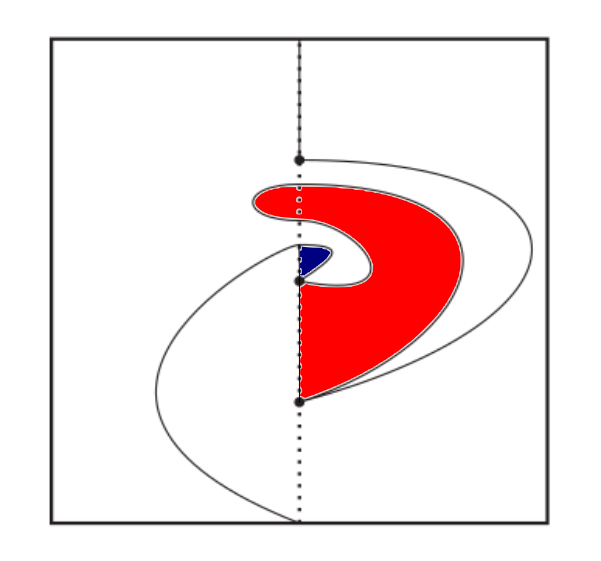
\includegraphics[width=7cm]{Images/biagonos.png}
		\end{center}\caption{Esse diagrama possui 2 biágonos (em vermelho e em azul), e pode ser reduzido ao diagrama da Figura \eqref{tranca disco perfurado}.}
		\label{diagrama nao reduzido com biagonos}
	\end{figure}
	\par\vspace{0.3cm} É, então, natural considerar os diagramas das Figuras \eqref{tranca disco perfurado} e \eqref{diagrama nao reduzido com biagonos} como equivalentes. Esse fato nos leva à seguinte definição.
	
	\begin{deff}
		\label{def equivalencia diagramas}
		Dois diagramas de curva são ditos equivalentes se têm a mesma forma reduzida.
	\end{deff}  
	\par\vspace{0.3cm} Vamos, agora, mostrar uma aplicação interessante dos diagramas de curva, a saber, na demonstração da Proposição \eqref{geradores de B_n tem ordem infinita}.
	\par\vspace{0.3cm} Dada uma trança $\beta$, vamos olhar para o seu diagrama de curva $c$. Começe na parte de baixo e observe o primeiro arco $c_i$ que não é igual ao arco correspondente $a_i$ no eixo. Se $c_i$ está à direita de $a_i$, dizemos que $\beta$ é \textit{desviada à direita} e, se $c_i$ está à esquerda de $a_i$, dizemos que $\beta$ é \textit{desviada à esquerda}. Se $c_i = a_i$ para todo $i$, então $\beta$ é a trança identidade (tecnicamente, estamos usando o Teorema \eqref{B_n isomorfo a Mod(D_n)}). A trança da Figura \eqref{tranca disco perfurado} é desviada à esquerda, pois começando na parte inferior, o arco $c_0$ desvia para a esquerda.
	\begin{prop}
		\label{desvio a direita desvio a esquerda}
		Se $\beta$ é desviada à esquerda, então $\beta^{-1}$ é desviada à direita.
	\end{prop}
	\begin{proof}
		O efeito, no diagrama de curva, de inverter uma trança é simplesmente realizar uma reflexão em torno de uma das arestas do disco paralelas ao eixo. Observe a Figura \eqref{diagrama inverso de sigma1}.
		\begin{figure}[H]
			\begin{center}
				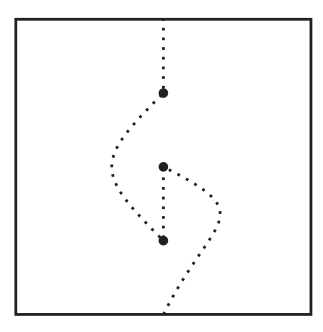
\includegraphics[width=5cm]{Images/inverso.png}
			\end{center}\caption{Diagrama de curva de $\sigma_1^{-1}$}\label{diagrama inverso de sigma1}
		\end{figure}
		\par\vspace{0.3cm} Portanto, como inverter uma trança equivale a refletir o seu diagrama de curva, segue que se a trança original era desviada à esquerda, o seu inverso será desviado à direita e vice-versa.
	\end{proof}
	\par\vspace{0.3cm} Queremos mostrar que $B_n$ é livre de torção. Esse fato segue do seguinte lema.
	
	\begin{lemma}
		\label{desviada a direita, sempre a direita}
		Se $\beta$ é desviada à direita, então $\beta^n$ é desviada à direita para todo $n>0$.
	\end{lemma}
	\begin{proof}
		Suponha que $\beta$ é desviada à direita, e observe o diagrama de curva reduzido $c$ de $\beta$. Encontre o primeiro $c_i$ que difere do $a_i$ correspondente, e chame esse arco de $c_k$. Denotando por $c^2$ o diagrama de curva de $\beta^2$, e por $c_i^2$ os arcos de $c^2$, imagine dois discos separados: um em que $a_i$ e $c_i$ estão desenhados e um em que $c_i$ e $c_i^2$ estão desenhados. Observe que a segunda figura é obtida da primeira aplicando a trança $\beta$ (pensada como um homeomorfismo). Então, como $c_k$ está à direita de $a_k$, segue que $c_k^2$ está à direita de $c_k$. Além disso, como não há biágonos na primeira figura, também não há biágonos na segunda figura.
		\par\vspace{0.3cm} Queremos mostrar que $\beta^2$ é desviada à direita, i.e, que $c_k^2$ está à direita de $a_k$. Sabemos que $\beta$ não afeta os arcos $a_i$ para $i<k$, e então $\beta^2$ também não. Também sabemos que, nas figuras, $c_k$ está à direita de $a_k$ e $c_k^2$ está à direita de $c_k$.
		\par\vspace{0.3cm} O que falta observar é que o diagrama de $\beta^2$ pode não estar reduzido. Sabemos que não há biágonos entre o eixo e $c$, e também que não há biágonos entre $c$ e $c^2$, mas se $c^2$ e o eixo formarem um biágono, então $c^2$ precisa ser reduzido e pode acabar não sendo desviado à direita.
		\par\vspace{0.3cm} Felizmente, isso não ocorre. Para ver que esse é o caso, seja $d$ o segmento inicial de $c_k$ que vai até a primeira vez que $c_k$ intercepta o eixo, de forma que $d$ está contido em uma metade (a metade da direita) do disco (é possível que $d$ seja $c_k$ inteiro, mas em geral $c_k$ pode "passear" bastante antes de atingir uma perfuração). Agora, a única maneira de $c_k^2$ estar à esquerda (ou ser igual) do arco $a_k$ do eixo é formando um biágono com $a_k$. Mas isso forçaria $c_k^2$ a cruzar $d$, criando um biágono entre $c$ e $c^2$, o que sabemos que não existe. Veja a figura abaixo.
		
		\begin{figure}[H]
			\begin{center}
				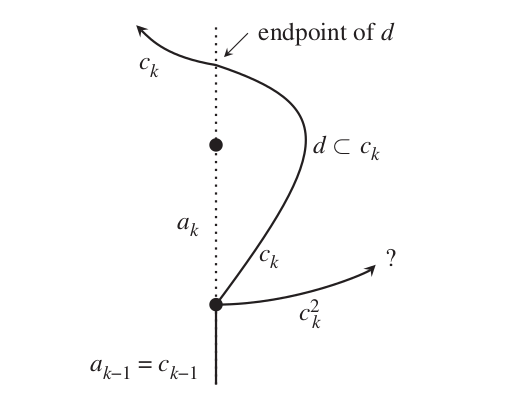
\includegraphics[width=8cm]{Images/demosntracao_lema.png}
			\end{center}\caption{Ilustração da demonstração}
			\label{ilustracao da demonstracao}
		\end{figure}
		\par\vspace{0.3cm} Portanto, $\beta^2$ é, de fato, desviada à direita. Repetindo o argumento, mostramos que $\beta^n$ é desviada à direita para todo $n>0$.
	\end{proof}
	
	\begin{corollary}
		\label{B_n livre de torcao por diagramas de curva}
		$B_n$ é livre de torção.
	\end{corollary}
	\begin{proof}
		Do Lema \eqref{desviada a direita, sempre a direita}, sabemos que se $\beta$ é desviada à direita, $\beta^n$ também o é para todo $n$ positivo. Da Proposição \eqref{desvio a direita desvio a esquerda}, sabemos que $\beta^{-1}$ é desviada à esquerda e então, novamente do Lema \eqref{desviada a direita, sempre a direita}, $(\beta^{-1})^n$ também o é para todo $n$ positivo. Portanto, toda trança que é desviada (seja à direita ou à esquerda) tem ordem infinita. Como, do Teorema \eqref{B_n isomorfo a Mod(D_n)}, a trança trivial é a única trança que não é desviada, temos que $B_n$ é livre de torção.
	\end{proof}
	
	\begin{remark}
		Na demonstração do Lema \eqref{desviada a direita, sempre a direita}, alguns detalhes foram omitidos. Por exemplo, homeomorfismos podem ser complicados: poderia ser o caso de que o arco $c_0$ interceptasse $a_0$ infinitas vezes. Então, como reduzi-lo? Esse e outros detalhes podem ser tratados de maneira rigorosa, o que está além do escopo desse relatório.
	\end{remark}
	
	\par\vspace{0.3cm} Uma última aplicação interessante dessa nova visualização dos grupos de trança é na identificação de tranças (palavras) que são equivalentes à identidade, ou seja, o problema da palavra (veja Seção \ref{secao o problema da palavra}). Usando o Teorema \eqref{B_n isomorfo a Mod(D_n)}, sabemos que uma trança $\beta$ é trivial se, e só se, $\psi(\beta) = \text{Id}$, ou seja, se, e só se, $\beta$ induz o homeomorfismo identidade (não faz nada com o disco). Portanto, dada uma trança $\beta$ qualquer, basta observarmos o efeito de $\beta$ no disco perfurado: se provoca torção, não é trivial; se não provoca torção, é trivial. Esse procedimento é complicado de computar para tranças longas, mas continua sendo uma solução igualmente válida.
	
	\chapter{Tranças e Teoria dos Nós}\label{secao trancas e teoria dos nos}
	\hspace{12pt} Vamos agora discutir algumas conexões entre tranças e a teoria dos nós.
	\par\vspace{0.3cm} Resumidamente, um nó é uma curva poligonal simples fechada em $\mathbb{R}^3$, mas para os propósitos desse relatório poderemos pensar em um nó como sendo uma curva suave simples, como os diagramas da figura \eqref{exemplos de nos}.
	
	\par\vspace{0.3cm} Os nós (ou, de modo mais geral, \textit{links}) e as tranças possuem semelhanças. Por exemplo, ambos são definidos em termos de figuras de cordas no espaço tridimensional, e ambos têm uma noção de equivalência, geralmente chamada de isotopia, que descreve quando duas figuras são equivalentes, ou seja, quando duas figuras representam o mesmo nó ou a mesma trança.  
	
	\begin{figure}[H]
		\begin{center}
			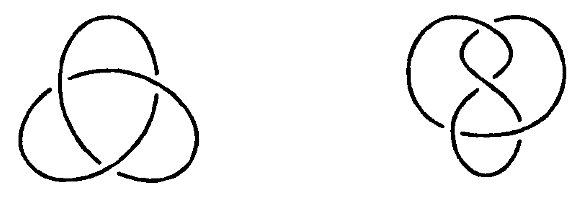
\includegraphics[width=7cm]{Images/exemplos_de_no.png}
		\end{center}\caption{Exemplos de nós}
		\label{exemplos de nos}
	\end{figure}
	
	\par\vspace{0.3cm} É claro que há algumas diferenças, a principal delas sendo o fato de que as tranças têm extremidades que não podem se mover durante isotopias, i.e., as extremidades ficam fixas conforme deformamos a trança, como vimos nas seções anteriores. Outra diferença é que cada corda de uma trança vai monotonicamente da esquerda para a direita, enquanto que não há essa restrição em relação aos \textit{links}. 
	\par\vspace{0.3cm} Na verdade, uma das primeiras motivações para o estudo das tranças era ajudar a entender a teoria dos nós e \textit{links}. A conexão é que toda trança pode ser "fechada" para formar um \textit{link}. Era esperado que a estrutura de grupo nas tranças levasse a algum tipo de estrutura de grupo no conjunto de \textit{links}, o que não acontece. Não obstante, há outras maneiras de usar tranças para ajudar com o estudo de \textit{links}.
	\par\vspace{0.3cm} Mas como formamos um \textit{link} a partir de uma trança? Fácil: basta ligar as extremidades sem introduzir novos cruzamentos.
	\par\vspace{0.3cm} Assim como fizemos para as tranças, também é possível alterar diagramas de nós através de deformações (ou movimentos) elementares (e seus respectivos inversos). Esses movimentos são chamados de \textit{movimentos de Reidemeister}, classificados em 3 tipos.
	
	\begin{figure}[H]
		\begin{center}
			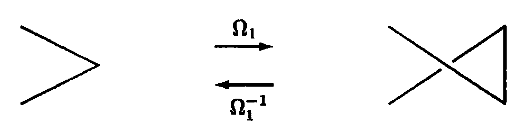
\includegraphics[width=10cm]{Images/reidemeister_1.png}
		\end{center}\caption{Movimento de Reidemeister do tipo I}
		\label{reidemeister tipo 1}
	\end{figure}
	
	\begin{figure}[H]
		\begin{center}
			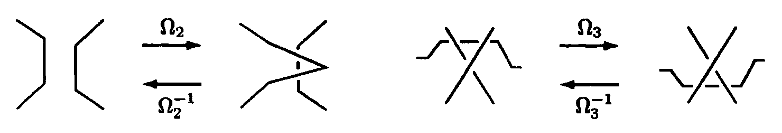
\includegraphics[width=14cm]{Images/reidemeister_2_e_3.png}
		\end{center}\caption{Movimentos de Reidemeister dos tipos II e III}
		\label{reidemeister tipos 2 e 3}
	\end{figure}
	\par\vspace{0.3cm} O teorema a seguir, que não será demonstrado, nos dá os análogos, para nós e \textit{links}, das relações de trança.
	
	\begin{theorem}
		\label{equivalencia de nos}
		Seja $K$ um nó (ou \textit{link}) e suponha que $D$ e $D'$ são dois diagramas de nó de $K$. Então, $D$ pode ser deformado em $D'$ através de uma sequência finita de movimentos de Reidemeister, ou seja, através de uma sequência finita das deformações $\Omega_1^{\pm1}, \Omega_2^{\pm1}$ e $\Omega_3^{\pm1}$. 
	\end{theorem}  
	
	\par\vspace{0.3cm} O Teorema \eqref{equivalencia de nos} nos dá um algoritmo conceitualmente muito simples para verificar se dois diagramas são, de fato, equivalentes, i.e., representam o mesmo nó: basta tentar todas as sequências possíves de movimentos em um dos diagramas e ver se o outro diagrama é produzido em alguma dessas sequências. Esse método de tentativa é válido pois recentemente foi provado que, dados dois diagramas, se um deles pode ser deformado no outro, ou seja, se eles representam o mesmo nó, então a quantidade de movimentos é limitada superiormente por uma função do número de cruzamentos no diagrama. Contudo, como esse limite superior é extremamente grande\footnote{Para detalhes, veja \cite{limite superior 1}, \cite{limite superior 2}, \cite{limite superior 3}}, esse algoritmo ainda não é prático. Ainda assim, os movimentos de Reidemeister são úteis para vários propósitos teóricos, como estabelecer vários invariantes de nós.
	\par\vspace{0.3cm} Os movimentos de Reidemeister, definidos para nós e \textit{links}, possuem análogos para as tranças. Esses análogos são os próprios movimentos de Reidemeister, com exceção do tipo I, uma vez que cada corda da trança deve ser monotônica. Isso significa que nunca podemos fazer um movimento do tipo I, pois não podemos ter \textit{loops}.  
	\par\vspace{0.3cm} Mas e os movimentos tipo II? Se, na trança, há uma parte que parece com o diagrama à esquerda da Figura \eqref{identidade b2}, então podemos endireitar ambas as cordas: esse é um movimento tipo II. Algebricamente, ele corresponde a cancelar $\sigma_i\sigma_i^{-1}$ (ou $\sigma_i^{-1}\sigma_i$) em uma palavra, o que é claro que podemos fazer. Também podemos sempre inserir tais pares sempre que quisermos, sem alterar a trança.
	\par\vspace{0.3cm} E os movimentos tipo III? Observe a Figura \eqref{trancas equivalentes}: ela é um movimento de Reidemeister tipo III!
	\par\vspace{0.3cm} De forma análoga ao Teorema \eqref{equivalencia de nos}, por meio de uma sequência de movimentos de Reidemeister dos tipos II e III, podemos partir de um diagrama de uma trança e chegar em qualquer outro diagrama de uma trança equivalente. Note, em particular, que esses movimentos (tipo II e tipo III) não alteram a paridade do número de cruzamentos. 
	\par\vspace{0.3cm} Voltando às conexões entre tranças e \textit{links} (e nós), lembre-se do que foi dito no início da seção: que fechando uma trança, obtemos um \textit{link}. De fato, não só podemos obter \textit{links} (e nós) a partir de tranças, como também podemos obter \textbf{todos} os \textit{links} a partir de tranças, como diz o seguinte teorema, que não será demonstrado aqui.
	
	\begin{theorem}[Alexander]
		\label{teorema de Alexander}
		Qualquer nó ou link $K$ pode ser representado como uma trança fechada.
	\end{theorem}
	
	\par\vspace{0.3cm} Uma consequência boa do Teorema \eqref{teorema de Alexander} é que temos uma maneira direta de descrever qualquer nó (e \textit{link}) sem precisar fazer um desenho. Em vez de dizer "é o nó que vai por cima, depois por baixo, e volta por trás para onde estava antes só que do outro lado e$\dots$", o que tem desvantagens óbvias, podemos simplesmente dizer "é o nó que obtemos fechando a trança de 3 cordas $\sigma_1\sigma_2^{-1}\sigma_1\sigma_2^2\sigma_1^2\sigma_2^3$". Muito mais simples.
	\par\vspace{0.3cm} Contudo, o Teorema \eqref{teorema de Alexander} não nos dá uma correspondência única entre tranças e \textit{links}. Várias tranças diferentes podem ser fechadas no mesmo \textit{link} e pode até ser o caso de que tranças com quantidades de cordas diferentes fechem no mesmo \textit{link}, como mostra a figura a seguir.
	
	\begin{figure}[H]
		\begin{center}
			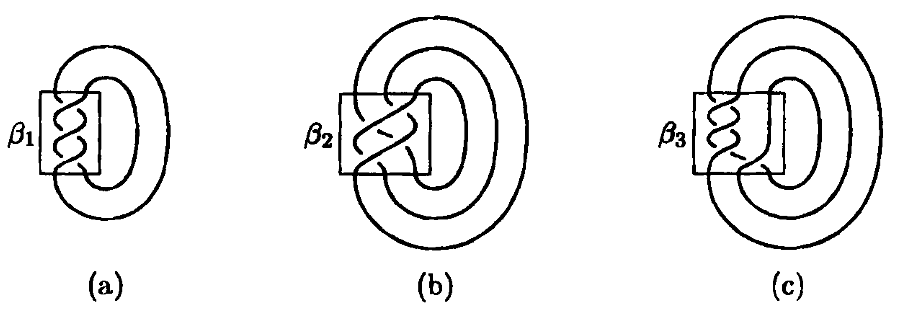
\includegraphics[width=12cm]{Images/fechamento_de_trancas_em_nos.png}
		\end{center}\caption{Tranças não equivalentes que fecham em nós equivalentes.}
		\label{fechamento de trancas em nos}
	\end{figure} 
	\par\vspace{0.3cm} Quando dois nós (ou \textit{links}) podem ser deformados um no outro, dizemos que eles são \textit{equivalentes} ou \textit{isotópicos}. Por exemplo, todas as tranças de $B_2(\mathbb{R}^2)$ (ou seja, todas as tranças de duas cordas) são fechadas no mesmo nó: o trivial.
	\par\vspace{0.3cm} Logo, se queremos estudar teoria dos nós via teoria das tranças, precisamos de um método para determinar se duas tranças fechadas são equivalentes, ou seja, se dois \textit{links} são isotópicos. De fato, a resposta para essa pergunta está no chamado \textit{teorema de Markov}, que será enunciado mais à frente.
	\par\vspace{0.3cm} Outro fato importante é que invariantes de trança podem não ser invariantes na trança fechada associada. Por exemplo, sabemos que dada uma trança $\beta$, $l$ (o homomorfismo de comprimento) é um invariante de $\beta$. Contudo, $l$ não precisa ser um invariante de $\widetilde{\beta}$, a trança fechada associada a $\beta$. Por exemplo, na Figura \eqref{fechamento de trancas em nos} $l(\beta_1) = 3 \neq 4 = l(\beta_2)$, mas $\widetilde{\beta_1}\sim\widetilde{\beta_2}$, i.e., os seus fechamentos são nós equivalentes.
	\par\vspace{0.3cm} Isso suscita a seguinte questão: existe um invariante de nó da trança fechada $\widetilde{\beta}$ que é definido a partir de um invariante da trança $\beta$?
	\par\vspace{0.3cm} A resposta é sim. Consideremos a permutação $\pi(\beta)$ associada à trança $\beta$. Sabemos que $\pi(\beta)$ pode ser expressa como produto de transposições, a saber
	\begin{align*}
	\pi(\beta) = C_1\cdots C_k
	\end{align*} 
	\par\vspace{0.3cm} Então $k$, que denotaremos por $\mu(\beta)$, é o número de componentes de $\widetilde{\beta}$ e um invariante do link $\widetilde{\beta}$, uma vez que o seguinte é válido:
	\begin{align*}
	\beta\sim\beta' \Rightarrow \pi(\beta) = \pi(\beta') \Rightarrow \mu(\beta) = \mu(\beta')
	\end{align*}
	\par\vspace{0.3cm} Portanto, $\widetilde{\beta}$ é um nó se, e somente se, $\pi(\beta)$ é um ciclo de ordem $n$, isto é, $\pi(\beta)$ não deixa pontos fixos. Nesse caso, dizemos que $\beta$ é uma trança fechada de um componente. Como um ciclo de ordem $n$ é escrito por um produto de $n-1$ transposições, então $\widetilde{\beta}$ é um nó se, e só se, $k = n-1$.
	\par\vspace{0.3cm} Note também que da maneira que definimos $\mu(\beta)$, é claro que, escrevendo $\beta = \sigma_{i_1}^{\varepsilon_1}\cdots\sigma_{i_k}^{\varepsilon_k}$, sendo $\varepsilon_i = \pm1$, temos como consequência imediata o fato de que $\mu(\beta) = \displaystyle{\sum_{i}^{k}|\varepsilon_i|}$. 
	\par\vspace{0.3cm} Até agora, vimos que a toda trança podemos associar um \textit{link}, mas que essa correspondência não é única (veja a Figura \eqref{fechamento de trancas em nos}). Esse fato levanta a questão: é possível dizer quando que o fechamento de duas tranças não equivalentes nos dá o mesmo \textit{link}? 
	\par\vspace{0.3cm} A resposta (em parte) é sim, contida no \textit{teorema de Markov} (ainda que não tenha sido o próprio Markov quem demonstrou). Mas o quê exatamente é o teorema de Markov?
	\par\vspace{0.3cm} Primeiro, vamos observar alguns fatos, como o lema a seguir.
	
	\begin{lemma}
		\label{conjugacoes dao o mesmo link}
		Sejam $\beta$ e $\gamma$ duas tranças de $n$ cordas. Então, o fechamento de $\beta$ e o fechamento de $\gamma\beta\gamma^{-1}$ nos dão o mesmo \textit{link}.
	\end{lemma}
	
	\begin{proof}
		A demonstração segue a ideia da Figura \eqref{conjugacao nao altera link}. Basicamente, fechando a trança $\gamma\beta\gamma^{-1}$, podemos mover a trança $\gamma^{-1}$ pelo \textit{link} de modo que tenhamos a trança $\beta\gamma^{-1}\gamma$, ou seja, a trança  $\beta$. Observe a figura.
		
		\begin{figure}[H]
			\begin{center}
				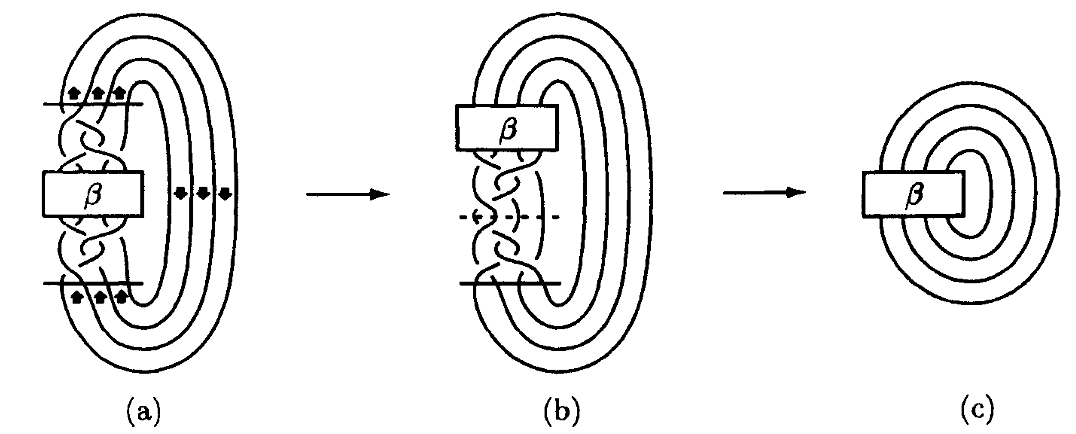
\includegraphics[width=12cm]{Images/conjugacao_nao_altera_link.png}
			\end{center}\caption{Conjugações não alteram o \textit{link}.}
			\label{conjugacao nao altera link}
		\end{figure}
	\end{proof}  
	\par\vspace{0.3cm} Por fim, antes de enunciarmos o teorema de Markov, suponha que $\beta$ é um trança de $n$ cordas e considere $\sigma_n$ um gerador de $B_{n+1}(\mathbb{R}^2)$. De maneira natural, se considerarmos $\beta$ como um elemento de $B_{n+1}(\mathbb{R}^2)$ em vez de $B_n(\mathbb{R}^2)$, podemos definir outras duas tranças de $n+1$ cordas,
	\[
	\begin{array}{ccc}
	\beta' = \beta\sigma_n & \text{e} & \beta'' = \beta\sigma_n^{-1}
	\end{array}
	\]
	\par\vspace{0.3cm} Nesse caso, $\beta$, $\beta'$ e $\beta''$ fecham no mesmo \textit{link}, como ilustra a figura abaixo. A figura (a) mostra o fecho de $\beta$, a figura (b), o fecho de $\beta\sigma_n$ e a (c), o fecho de $\beta\sigma_n^{-1}$.
	
	\begin{figure}[H]
		\begin{center}
			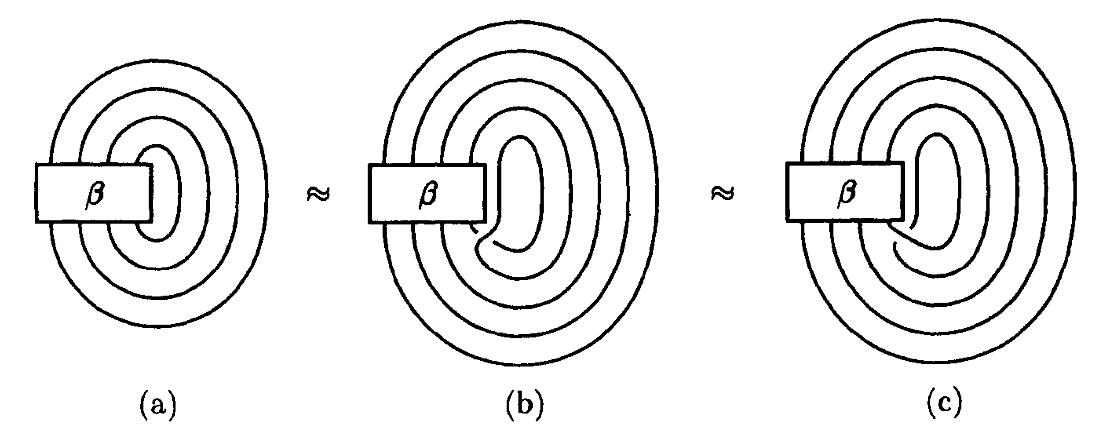
\includegraphics[width=13cm]{Images/movimentos_de_markov.png}
		\end{center}\caption{Movimentos de Markov}
		\label{movimentos de Markov}
	\end{figure}
	\par\vspace{0.3cm} É claro que há outras maneiras de obter tranças cujos fechos representam o mesmo \textit{link}, mas, como veremos adiante, as duas tranformações acima mostradas nas Figuras \eqref{conjugacao nao altera link} e \eqref{movimentos de Markov} são especiais. Como foi Markov quem primeiro as introduziu, elas são usualmente chamadas de \textit{movimento de Markov tipo I} e \textit{movimentos de Markov tipo II}. Vamos defini-los formalmente.
	\begin{deff}
		\label{def movimento de Markov tipo 1}
		Um movimento de Markov tipo I, denotado $M_1$, substitui uma trança $\beta$ de $n$ cordas pelo seu conjugado $\gamma\beta\gamma^{-1}$, sendo $\gamma$ uma trança de $n$ cordas arbitrária.  
	\end{deff}
	\begin{deff}
		\label{def movimento de Markov tipo 2}
		Um movimento de Markov do tipo II, denotado $M_2$, substitui a trança $\beta$ de $n$ cordas pela trança $\beta\sigma_n$ ou $\beta\sigma_n^{-1}$ de $n+1$ cordas, sendo $\beta$ visualizada com uma trança de $B_{n+1}(\mathbb{R}^2)$ e $\sigma_n$ um gerador de $B_{n+1}(\mathbb{R}^2)$. 
	\end{deff}
	\par\vspace{0.3cm} É claro que podemos definir também os inversos de $M_1$ e $M_2$, que denotaremos por $M_1^{-1}$ e $M_2^{-1}$, respectivamente. Agora, estamos prontos para enunciar o teorema (que não será demonstrado).
	
	\begin{theorem}[Markov]
		\label{teorema de Markov}
		Suponha $\beta$ e $\beta'$ duas tranças (orientadas) não necessariamente com o mesmo número de cordas. Então, os fechos de $\beta$ e $\beta'$ representam o mesmo \textit{link} ou nó $K$ (orientado) se, e somente se, $\beta$ pode ser deformada em $\beta'$ por uma sequência finita dos movimentos $M_1^{\pm1}, M_2^{\pm1}$. Em símbolos, existe a seguinte sequência finita,
		\begin{align*}
		\beta = \beta_0\to\beta_1\to\cdots\to\beta_m = \beta',
		\end{align*}
		\par\vspace{0.3cm} tal que, para $i = 0,1,\dots,m-1$, $\beta_{i+1}$ é obtida a partir de $\beta_i$ pela aplicação de um dos movimentos $M_1^{\pm1}$ e $M_2^{\pm1}$.
	\end{theorem}
	\par\vspace{0.3cm} Podemos, ainda, pensar nos movimentos de Markov para as tranças como paralelos diretos dos movimentos de Reidemeister para \textit{links}. Por conveniência, diremos que duas tranças $\beta$ e $\beta'$ são \textit{Markov equivalentes}, denotado por $\beta\underset{M}{\sim}\beta'$, se uma pode ser deformada na outra por meio de uma sequência finita de movimentos de Markov. De fato,
	\begin{prop}
		\label{Markov equivalencia}
		Markov equivalência é uma relação de equivalência.
	\end{prop}  
	\begin{proof}
		Sejam $\alpha$, $\beta$ e $\gamma$ tranças quaisquer, não necessariamente com o mesmo número de cordas. Note que 
		\begin{align*}
		\alpha = \alpha_0\overset{M_1}{\to}\alpha_1\overset{M_1^{-1}}{\to}\alpha_2 = \alpha
		\end{align*}
		\par\vspace{0.3cm} logo $\alpha\underset{M}{\sim}\alpha$ e, portanto, a relação $\underset{M}{\sim}$ é reflexiva.
		\par\vspace{0.3cm} Agora, suponha que $\alpha\underset{M}{\sim}\beta$. Então, por definição, existe uma sequência finita
		\begin{align*}
		\alpha\to\cdots\to\beta 
		\end{align*}
		\par\vspace{0.3cm} de movimentos de Markov que nos permite deformar $\alpha$ em $\beta$. Consequentemente, podemos partir de $\beta$ e, usando a mesma sequência, só que de trás para frente, chegar em $\alpha$. Portanto, $\alpha\underset{M}{\sim}\beta$ implica $\beta\underset{M}{\sim}\alpha$ e a relação $\underset{M}{\sim}$ é simétrica.
		\par\vspace{0.3cm} Por fim, suponha $\alpha\underset{M}{\sim}\beta$ e $\beta\underset{M}{\sim}\gamma$. Por definição, existem duas sequências finitas, $S_1$ e $S_2$, digamos, 
		\begin{align*}
		\alpha\overset{S_1}{\to}\beta \\
		\beta\overset{S_2}{\to}\gamma 	
		\end{align*}
		\par\vspace{0.3cm} e, consequentemente, existe uma sequência finita $S_3$ de $\alpha$ em $\gamma$
		\begin{align*}
		\alpha\overset{S_1}{\to}\beta\overset{S_2}{\to}\gamma 
		\end{align*}
		\par\vspace{0.3cm} sendo $S_3$ a sequência $S_1$ seguida de $S_2$. Portanto, $\underset{M}{\sim}$ é transitiva e configura uma relação de equivalência.
	\end{proof}
	\par\vspace{0.3cm} Com a noção de Markov equivalência, podemos reescrever o Teorema \eqref{teorema de Markov} da seguinte forma.
	\begin{theorem}[Markov simplificado]
		\label{teorema de Markov simplificado}
		Sejam $\widetilde{\beta}$ e $\widetilde{\beta'}$ dois \textit{links} (ou nós). Então, $\widetilde{\beta}$ é equivalente a $\widetilde{\beta'}$ se, e somente se, $\beta\underset{M}{\sim}\beta'$.
	\end{theorem}
	\par\vspace{0.3cm} Algumas obeservações são necessárias.
	\begin{remark}
		Primeiro, note que o Teorema \eqref{teorema de Markov}, em si, não é suficiente para classificarmos todos os \textit{links} e nós. O obstáculo é que, atualmente, não existe nenhum algoritmo conhecido para determinar se duas tranças $\beta$ e $\beta'$ são Markov equivalentes ou não. Dito isso, nos casos relativamente simples de tranças de 2 ou 3 cordas, se os fechos de $\beta$ e $\beta'$ são equivalentes, então (a menos de uma família de tranças de 3 cordas que já foi completamente classificada) $\beta$ e $\beta'$ são conjugadas.\cite{classificacao}
		\par\vspace{0.3cm} Segundo, tenha em mente que nos restringimos a \textit{links} e nós \textbf{orientados}. Se ignorarmos a orientação, o teorema de Markov pode não valer. Por exemplo, considere a figura abaixo.
		
		\begin{figure}[H]
			\begin{center}
				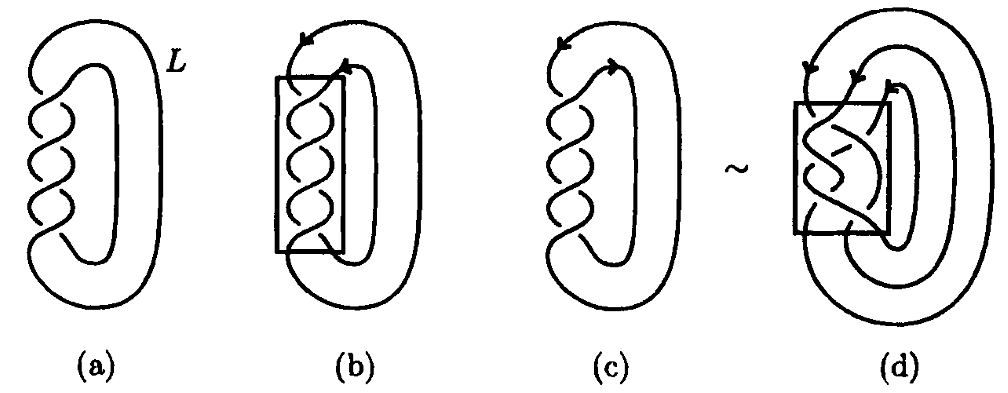
\includegraphics[width=12cm]{Images/orientacao_markov_link.png}
			\end{center}\caption{O \textit{link} $L$ e duas orientações possíveis.}\label{orientacao markov link}
		\end{figure}
		\par\vspace{0.3cm} Se orientarmos $L$ como na Figura \eqref{orientacao markov link}(b), então (o \textit{link} orientado) $L$ é o fecho da trança de 2 cordas $\sigma_1^4$. Por outro lado, se orientarmos $L$ como na Figura \eqref{orientacao markov link}(c), então o mesmo \textit{link} $L$ não pode ser o fecho de nenhuma trança de 2 cordas. Mas, de fato, é possível mostrar que com essa orientação, $L$ na verdade é o fecho da trança de 3 cordas $\sigma_1^{-1}\sigma_2\sigma_1^{2}\sigma_2^{1}$, Figura \eqref{orientacao markov link}(d).
		\par\vspace{0.3cm} Portanto, o \textit{link} (não orientado) $L$ da Figura \eqref{orientacao markov link}(a) pode ser representado por duas tranças distintas, $\sigma_1^4$ e $\sigma_1^{-1}\sigma_2\sigma_1^{2}\sigma_2^{1}$. Contudo, essas duas tranças \textbf{não} são Markov equivalentes. 
		\par\vspace{0.3cm} Outro exemplo é o da Figura \eqref{orientacao markov no}.
		
		\begin{figure}[H]
			\begin{center}
				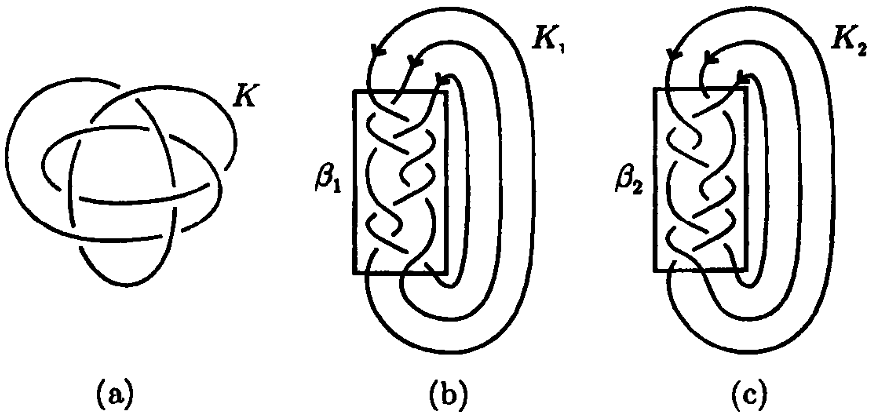
\includegraphics[width=9cm]{Images/orientacao_markov_no.png}
			\end{center}\caption{O nó $K$ e duas orientações possíveis.}\label{orientacao markov no}
		\end{figure}
		
		\par\vspace{0.3cm} É sabido, mas não é fácil mostrar, que os nós (orientados) $K_1$ e $K_2$ da Figura \eqref{orientacao markov no}, apesar de obtidos a partir do mesmo nó não orientado $K$, não são equivalentes, justamente por serem dados por orientações diferentes. Pela figura, $K_1$ e $K_2$ são representados pelas tranças $\beta_1$ e $\beta_2$, respectivamente. Como $K_1$ e $K_2$ não são equivalentes, então $\beta_1$ e $\beta_2$ não são Markov equivalentes.  
		
	\end{remark}
	\section{Algumas aplicações do Teorema de Markov}
	\hspace{12pt} Seja $K$ um nó (ou \textit{link}) orientado em $\mathbb{R}^3$. Se considerarmos o plano $xy$ como um espelho, então a imagem de $K$ nesse espelho também é um nó em $\mathbb{R}^3$, veja a figura abaixo.
	
	\begin{figure}[H]
		\begin{center}
			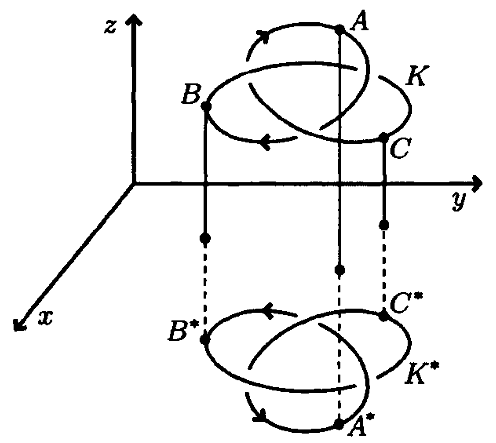
\includegraphics[width=6cm]{Images/no_espelhado.png}
		\end{center}\caption{O nó $K$ refletido em torno do plano $xy$.}\label{no espelhado}
	\end{figure}
	\par\vspace{0.3cm} O nó $K^\ast$ é chamado de imagem espelhada de $K$. Como $K$ é orientado, $K^\ast$ herda uma orientação de $K$.
	\begin{prop}
		\label{troca de cruzamentos}
		Seja $D$ um diagrama (orientado) de um nó $K$. Então, o diagrama $D^\ast$ do nó $K^\ast$ é obtido de $D$ substituindo cruzamentos superiores por cruzamentos inferiores.	
	\end{prop}
	\begin{proof}
		Como a imagem espelhada de $K$ é obtida a partir de uma rotação de $K$, então os cruzamentos superiores passam a ser inferiores e vice-versa.
	\end{proof}
	\par\vspace{0.3cm} Na Figura \eqref{no de trevo} abaixo estão representados os diagramas $D$ e $D^\ast$ de um nó $K$. Esse nó $K$ é chamado de \textit{nó de trevo}.
	
	\begin{figure}[H]
		\begin{center}
			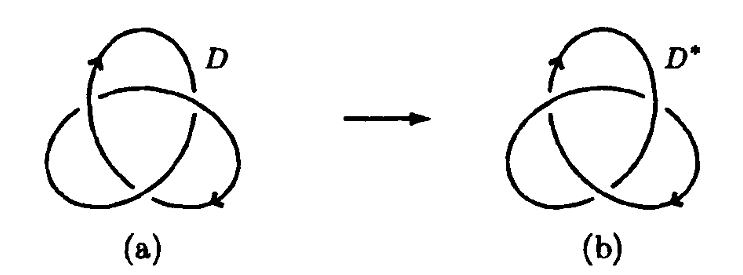
\includegraphics[width=9cm]{Images/no_de_trevo.png}
		\end{center}\caption{O nó de trevo orientado.}
		\label{no de trevo}
	\end{figure} 
	
	\par\vspace{0.3cm} Apesar de que, em geral, um nó e sua imagem espelhada não são equivalentes, há casos em que isso acontece. Um nó que é equivalente a sua imagem espelhada é chamado de \textit{anfiquiral} ou \textit{aquiral}. Um exemplo de nó aquiral é o nó da figura abaixo.
	
	\begin{figure}[H]
		\begin{center}
			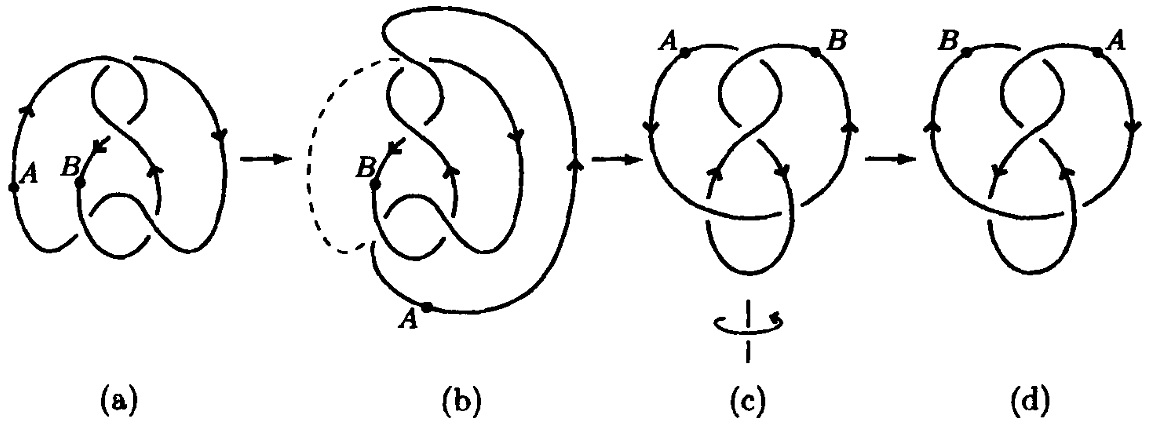
\includegraphics[width=11cm]{Images/no_aquiral.png}
		\end{center}\caption{O nó figura oito, um exemplo de nó aquiral.}\label{no aquiral}
	\end{figure}
	
	\par\vspace{0.3cm} O nó da Figura \eqref{no aquiral}(a), representado pelo diagrama $D$, pode ser representado pelo fecho da trança de $3$ cordas $\beta = \sigma_1\sigma_2^{-1}\sigma_1\sigma_2^{-1} = (\sigma_1\sigma_2^{-1})^2$. Na sua forma de trança, a imagem espelhada $K^\ast$ de $K$ é exatamente o fecho da trança $\beta^{-1}$ (com a orientação inversa), como mostra a figura abaixo.
	
	\begin{figure}[H]
		\begin{center}
			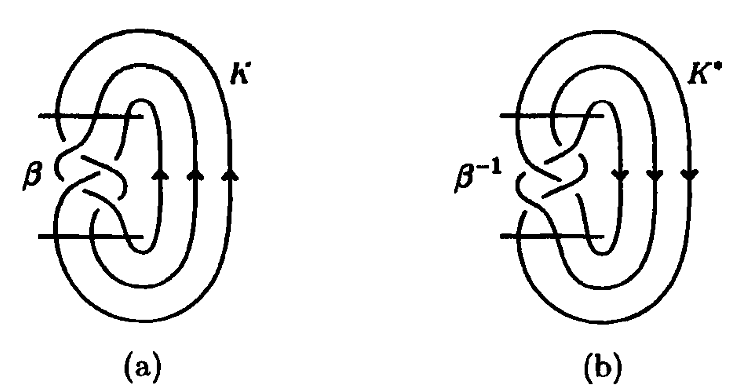
\includegraphics[width=10cm]{Images/tranca_no_de_oito.png}
		\end{center}\caption{Trança do nó figura oito.}\label{tranca no de oito}
	\end{figure} 
	
	\par\vspace{0.3cm} Esse exemplo suscita a pergunta: dado um nó (ou \textit{link}) orientado e uma trança que representa esse nó, como podemos expressar $K^\ast$ baseados em $\beta$? A resposta está na proposição a seguir.
	
	\begin{prop}
		\label{representacao no espelhado}
		Seja $K$ um nó (ou \textit{link}) orientado e suponha que $K$ é o fecho de uma trança de $n$ cordas $\beta = \sigma_{i_1}^{\varepsilon_1}\cdots\sigma_{i_k}^{\varepsilon_k}$, sendo $1\leq i_1, i_2, \dots, i_k\leq n-1$ e $\varepsilon_i=\pm1$. Então, 
		\begin{enumerate}
			\item a imagem espelhada $K^\ast$ de $K$, com a orientação invertida, pode ser representada como o fecho de 
			$\beta^{-1}  = \sigma_{i_k}^{-\varepsilon_{k}}\cdots\sigma_{i_1}^{-\varepsilon_1}$ 
			\item o nó $\overline{K}$ obtido de $K$ revertendo a orientação de $K$ pode ser representado por
			
			\begin{align*}
			\overline{\beta} = \sigma_{i_k}^{\varepsilon_k}&\cdots\sigma_{i_i}^{\varepsilon_1} \\
			&\text{ou} \\
			\overline{\overline{\beta}} = \sigma_{n-i_k}^{\varepsilon_k}&\cdots\sigma_{n - i_1}^{\varepsilon_1}
			\end{align*}
			\par\vspace{0.3cm} e, portanto, $\overline{\beta}\underset{M}{\sim}\overline{\overline{\beta}}$. 
		\end{enumerate}
	\end{prop}
	
	\begin{proof}
		A demonstração do item 1 segue diretamente dos diagramas da Figura \eqref{tranca no de oito}. De fato, inverter a orientação de $K$ equivale a espelhar a trança $\beta$, ou seja, invertê-la. Para o item 2, observe a Figura \eqref{no invertido}, que ilustra o processo aqui descrito. Primeiro, mude a orientação da Figura \eqref{no invertido}(a) para obter a Figura \eqref{no invertido}(b). Então, vire a Figura \eqref{no invertido}(b) de cabeça para baixo, Figura \eqref{no invertido}(c). Em seguida, rotacione a Figura \eqref{no invertido}(c) em torno do eixo vertical por um ângulo de $\pi$ radianos, Figura \eqref{no invertido}(d). Podemos ver que a Figura \eqref{no invertido}(c) é $\overline{\overline{\beta}}$ e que a Figura \eqref{no invertido}(d) é $\overline{\beta}$. Como não alteramos o nosso nó $\overline{K}$, então os fechos de $\overline{\beta}$ e $\overline{\overline{\beta}}$ são equivalentes e representam o mesmo nó, $\overline{K}$. Por fim, pelo Teorema \eqref{teorema de Markov simplificado}, temos $\overline{\beta}\underset{M}{\sim}\overline{\overline{\beta}}$.
		
		\begin{figure}[H]
			\begin{center}
				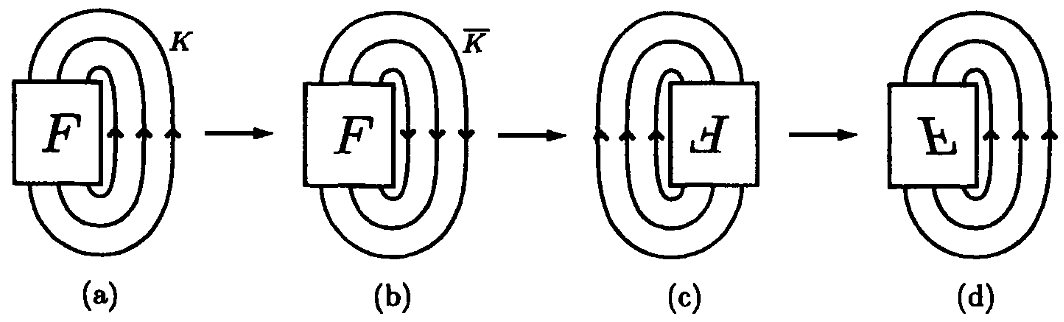
\includegraphics[width=12cm]{Images/no_invertido.png}
			\end{center}\caption{Inversão da orientação de um nó.}\label{no invertido}
		\end{figure}
		
		\par\vspace{0.3cm} 
		
	\end{proof}
	\par\vspace{0.3cm} Se os nós $K$ e $\overline{K}$ são equivalentes, então $K$ é dito \textit{inversível}. O nó da Figura \eqref{no aquiral}(a) é inversível, uma vez que os dois nós das Figuras \eqref{no aquiral}(c) e (d) são equivalentes. Apesar de muitos nós serem inversíveis, isso não quer dizer que todos os nós o são. De fato, um contraexemplo é o nó $K$ da Figura \eqref{orientacao markov no}.
	%COMECEI AQUI
	\section{Grupos de nó}
	\hspace{12pt} Até agora, tratamos de nós de maneira um tanto quanto informal. Contudo, assim como fizemos para a trança, podemos tomar uma abordagem mais topológica. De fato, podemos utilizar, assim como foi com as tranças, grupos fundamentais. Para isso, recorde que definimos nó como uma curva poligonal simples fechada em $\mathbb{R}^3$. Contudo, por conveniência, é comum substituir $\mathbb{R}^3$ por $\mathbb{S}^3$ (a 3-esfera unitária), pois $\mathbb{S}^3$ pode ser obtida de $\mathbb{R}^3$ adicionando um único ponto (de fato, isso é verdade para $\mathbb{S}^n$ e $\mathbb{R}^n$, realizando-se um análogo da projeção estereográfica para dimensões superiores. Como exercício, imagine o caso $n = 1$. Informalmente, estamos adicionando a $\mathbb{R}$ o "ponto infinito", $\infty$.)
	\par\vspace{0.3cm} Nesse contexto, podemos definir o \textit{complemento de um nó}.
	\begin{deff}
		\label{def complemento no}
		Dado um nó $K$, o complemento de $K$ é o subconjunto $\mathbb{S}^3 - K$ de $\mathbb{S}^3$.
	\end{deff}
	\par\vspace{0.3cm} Com essa definição, podemos então definir o \textbf{grupo fundamental do complemento de nó}, muitas vezes chamado simplesmente de \textbf{grupo fundamental de nó}.
	\begin{deff}
		\label{grupo fundamental de no}
		O grupo fundamental de um nó $K$ com ponto base $b\in\mathbb{S}^3 - \text{Im}(K)$ é o grupo fundamental do complemento de $K$, com $b$ como ponto base.
	\end{deff}
	\par\vspace{0.3cm} Como $\mathbb{S}^3$ é conexo por caminhos, podemos omitir o ponto base, pois a escolha dele não afeta a estrutura de grupo. Em síbolos, denotamos o grupo fundamental do nó $K$ por $\pi_1(\mathbb{S}^3\setminus K)$. 
	\par\vspace{0.3cm} Um primeiro exemplo é o grupo fundamental do nó trivial. Apesar do nó ser trivial, seu grupo não o é; de fato, o grupo fundamental do nó trivial é o grupo cíclico infinito, $\mathbb{Z}$. Outro exemplo é o nó de trevo, mostrado na figura \eqref{no de trevo}; o seu grupo fundamental tem apresentação 
	\begin{align*}
	\langle x,y|x^3 = y^2 \rangle
	\end{align*}
	\par\vspace{0.3cm} ou seja, o grupo do nó de trevo é (isomorfo a) $B_3(\mathbb{R}^2)$! Um último exemplo é o nó figura oito, mostrado na figura \eqref{no aquiral}; seu grupo fundamental tem apresentação
	\begin{align*}
	\langle x,y | yxy^{-1}xy = xyx^{-1}yx \rangle
	\end{align*}
	\par\vspace{0.3cm} O grupo fundamental de nó também é um invariante: se dois nós são equivalentes, então seus grupos fundamentais são isomorfos. Contudo, o contrário não é verdadeiro. Por exemplo, os dois nós de trevo abaixo têm o mesmo grupo fundamental, mas não são equivalentes (pois o nó de trevo é quiral, como vimos).
	
	\begin{figure}[H]
		\begin{center}
			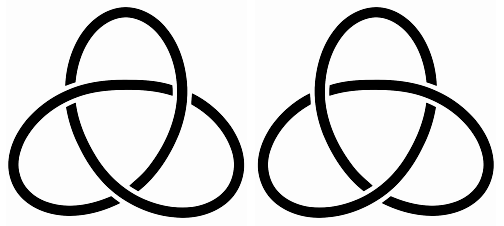
\includegraphics[width=6cm]{Images/nos_de_trevo.png}
		\end{center}\caption{Os nós de trevo destro (à esquerda) e canhoto (à direita).}\label{nos de trevo destro e canhoto}
	\end{figure} 
	
	\par\vspace{0.3cm} Uma das maiores questões quando estudamos nós é determinar se dois nós são ou não equivalentes, ou seja, como podemos distinguir dois nós. Uma das ferramentas que nos ajuda nessa tarefa são os chamados \textit{invariantes de nós}. Demos um exemplo de invariante de nó acima, a saber, o número de componentes $\mu(\beta)$. Esse invariante era, de certo modo, esperado, uma vez que não podemos "cortar" nosso nó, ou seja, é impossível alterar o número de componentes por meio de movimentos de Reidemeister ($\Omega_1^{\pm1}$, $\Omega_2^{\pm1}$ e $\Omega_3^{\pm1}$). Outros exemplos de invariantes são o polinômio de Alexander e o polinômio de Jones, que serão abordados a seguir. Antes, porém, uma curiosidade.
	\par\vspace{0.3cm} Um tipo particular de nó são os chamados \textit{nós de toro} (ou \textit{nós torais}). Como o nome sugere, são nós que pertencem à superfície de um toro (que, por sua vez, é um subconjunto de $\mathbb{R}^3$). Podemos definir um nó de toro usando coordenadas da seguinte forma.\footnote{Veja \cite{no toral}.}
	
	\begin{deff}
		\label{def no de toro}
		Para todo par de inteiros $a$ e $b$ coprimos, o nó de toro padrão $K_{a,b}: \mathbb{S}^1\to\mathbb{S}^3$ correspondente ao par $(a,b)$ é dado, em coordenadas Euclidianas, por 
		\begin{align*}
		\theta\mapsto
		\left( 
		\begin{matrix}
		(2+\cos(b\theta))\cos(a\theta) \\
		(2+\cos(b\theta))\sin(a\theta) \\
		-\sin(a\theta)
		\end{matrix} 
		\right)
		\end{align*}	
	\end{deff}
	\par\vspace{0.3cm} Essa função é uma imersão do círculo ($\mathbb{S}^1$) no toro $T$ parametrizado por
	\begin{align*}
	(\theta, \varphi)\mapsto 
	\left( \begin{matrix}
	(2+\cos(\theta))\cos(\varphi) \\
	(2+\cos(\theta))\sin(\varphi) \\
	\sin(\theta)
	\end{matrix}  \right)
	\end{align*}
	\begin{figure}[H]
		\begin{center}
			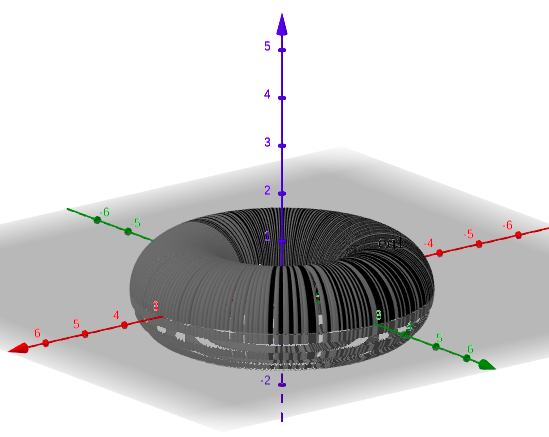
\includegraphics[width=8cm]{Images/toro.png}
		\end{center}\caption{O toro $T$ em $\mathbb{R}^3$.}\label{toro}
	\end{figure}
	\par\vspace{0.3cm} Os exemplos mais simples de nós torais são os nós de toro $K_{2,3}$ e $K_{2,-3}$, que são os nós de trevo destro e canhoto, respectivamente. Note que os nós de trevo ficam completamente contidos na superfície do toro $T$, assim como todos os nós torais. Em particular, se $a = \pm1$ ou se $b = \pm1$, então o nó $K_{a,b}$ resultante é trivial.
	
	\begin{figure}[H]
		\centering
		\begin{subfigure}[t]{0.5\textwidth}
			\centering
			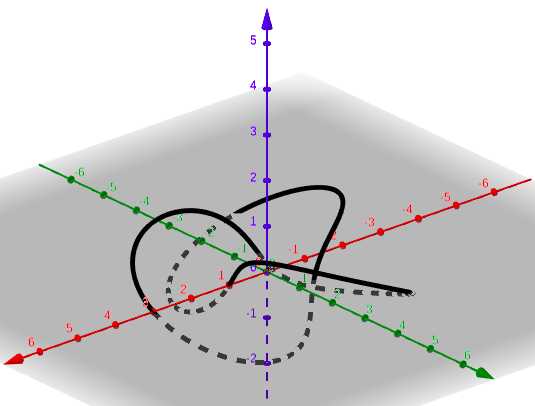
\includegraphics[width=6cm,height=5cm]{Images/no_de_trevo_parametrizado.png}
			\caption{}
		\end{subfigure}%
		~ 
		\begin{subfigure}[t]{0.5\textwidth}
			\centering
			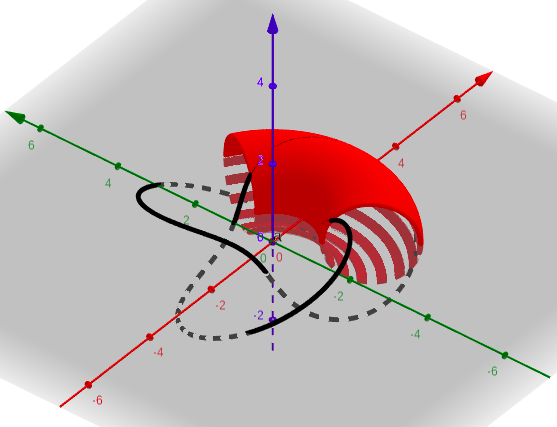
\includegraphics[width=6cm,height=5cm]{Images/no_de_trevo_no_toro.png}
			\caption{}
		\end{subfigure}
		\caption{O nó toral $K_{2,3}$ (nó de trevo destro), figura (a) e parte do toro, envolvendo $K_{2,3}$, figura (b)}
	\end{figure}
	%\newpage
	\par\vspace{0.3cm} É interessante observar que, sem a restrição de $(a,b)$ coprimos, a função de $K_{a,b}:\mathbb{S}^1\to\mathbb{S}^3$ descreve um \textit{link}. Logo, podemos generalizar a Definição \eqref{def no de toro} para \textit{links}, da seguinte forma.
	\begin{deff}
		\label{def link de toro}
		Para todo par de inteiros $a$ e $b$ (não necessariamente coprimos), o \textit{link} de toro (ou link toral) padrão $K_{a,b}: \mathbb{S}^1\to\mathbb{S}^3$ correspondente ao par $(a,b)$ é dado, em coordenadas Euclidianas, por 
		\begin{align*}
		\theta\mapsto
		\left( 
		\begin{matrix}
		(2+\cos(b\theta))\cos(a\theta) \\
		(2+\cos(b\theta))\sin(a\theta) \\
		-\sin(a\theta)
		\end{matrix} 
		\right)
		\end{align*}
		\par\vspace{0.3cm} O número de componentes do link correspondente ao par $(a,b)$ é dado por $d = \mdc(a,b)$, e cada componente é uma cópia do nó $\displaystyle{K_{a/d, b/d}}$ rotacionado em torno do eixo $z$.
	\end{deff}
	\par\vspace{0.3cm} Uma propriedade interessante é que todo nó toral não trivial é quiral, i.e., não é igual à sua imagem espelhada (daí a nomenclatura "destro" e "canhoto"). Por fim, vale mencionar que todo nó toral $K_{a,b}$ pode ser representado pela trança fechada $(\sigma_1\sigma_2\cdots\sigma_{a-1})^b$.  
	
	\subsection{Cálculo do grupo de nó}
	\hspace{12pt} Como dito antes, dados dois nós equivalentes $K_1$ e $K_2$, então $\pi_1(\mathbb{R}^3\setminus K_1) \cong \pi_1(\mathbb{R}^3\setminus K_2)$. Contudo, novamente, a recíproca não é verdadeira: $\pi_1(\mathbb{R}^3\setminus K_1) \cong \pi_1(\mathbb{R}^3\setminus K_2)$ não implica $K_1$ e $K_2$ equivalentes. 
	\par\vspace{0.3cm} Se queremos usar os grupos de nó para obter informações acerca dos nós, devemos ser capazes de efetivamente determinar esses grupos. Felizmente, existe um algoritmo simples, introduzido por Wirtinger por volta de 1904 em suas aulas em Vienna e publicado em 1908 por Tietze. Vamos descrever o \textbf{método de Wirtinger}.
	\subsubsection*{Algoritmo de Wirtinger}
	\hspace{12pt} Suponha que temos uma projeção de nó.
	\begin{enumerate}
		\item Fixe uma direção ao longo de $K$ e denote os arcos sucessivos entre dois cruzamentos inferiores por $\alpha_1, \dots, \alpha_n$.
		\item Para $1\leq i\leq n$, desenhe um seta curta $x_i$ passando por baixo de $\alpha_i$, em que a direção de $x_i$ é dada pela regra da mão direita, com o dedão apontando na direção escolhida sobre $K$. Tal seta representa um \textit{loop} em $\mathbb{R}^3\setminus K$ do seguinte modo: tome um ponto base acima do plano de desenho; então o \textit{loop} consiste do triângulo orientado a partir do ponto base para a cauda de $x_i$, ao longo de $x_i$ até a ponta e de volta para o ponto base.
		\begin{figure}[H]
			\begin{center}
				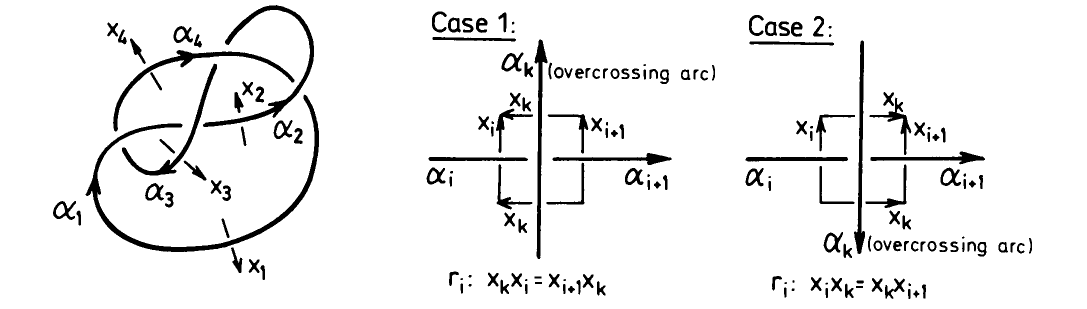
\includegraphics[width=15cm]{Images/arcosgrupono.png}
			\end{center}\caption{Desenhos possíveis}
			\label{desenhos possiveis}
		\end{figure}
		\item Em cada cruzamento, indique o quadrado formado pelas setas sob os arcos envolvidos no cruzamento, e escreva a relação $r_i$ indicada por esse quadrado; há duas possibilidades dadas pelos desenhos na Figura \eqref{desenhos possiveis}(note que $k=i$ ou $k=i+1$ é possível)
		\par Então o grupo do nó $K$ é gerado por (classes de homotopia de) \textit{loops} $x_i$ e tem apresentação
		\begin{align*}
		\tag{Apresentação de Wirtinger}
		\pi_1(\mathbb{R}^3\setminus K) = \left< x_1, \dots, x_n \ | \ r_1, \dots, r_n \right>
		\end{align*}
		\par Ademais, qualquer das relações $r_i$ é consequência das $n-1$ relações restantes e pode, portanto, ser omitida.
	\end{enumerate}
	\par\vspace{0.3cm} Não vamos, aqui, demonstrar precisamente o teorema, mas vamos dar algumas observações. É razoavelmente claro, geometricamente, que $\pi_1(\mathbb{R}^3\setminus K)$ é gerado pelos \textit{loops} $x_i$; para qualquer \textit{loop} em $\mathbb{R}^3\setminus K$, basta checar quantas voltas ele dá em cada um dos arcos $\alpha_i$ e deformá-lo conformemente. Também é claro que as relações $r_i$ devem valer, i.e., que $x_kx_ix_k^{-1}x_{i+1}^{-1}$ (caso 1) ou $x_ix_kx_{i+1}^{-1}x_k^{-1}$ (caso 2) podem ser reduzidas a um ponto em $\mathbb{R}^3\setminus K$. Isso é mostrado nas seguintes figuras.
	\begin{figure}[H]
		\begin{center}
			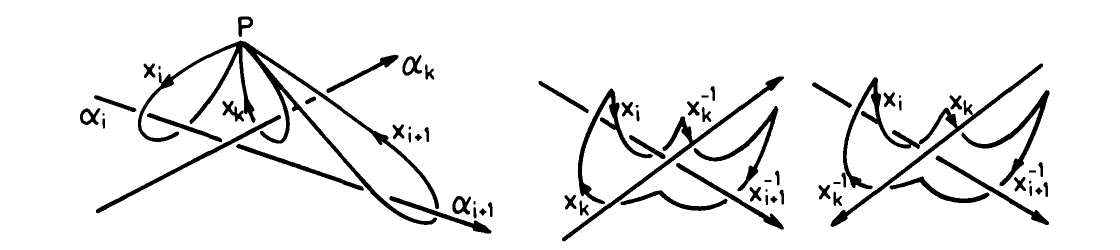
\includegraphics[width=15cm]{Images/deformacaoloops.png}
		\end{center}\caption{Redução em cada caso}
	\end{figure}
	\par\vspace{0.3cm} O que não é tão óbvio é que nenhuma relação adicional vale e que qualquer uma das $n$ relações pode ser omitida. Vamos olhar os dois exemplos dados acima, do nó de trevo e do nó figura oito, mais de perto.
	\begin{example}[Nó de trevo]
		Seja $K$ o nó de trevo dado abaixo.
		\begin{figure}[H]
			\begin{center}
				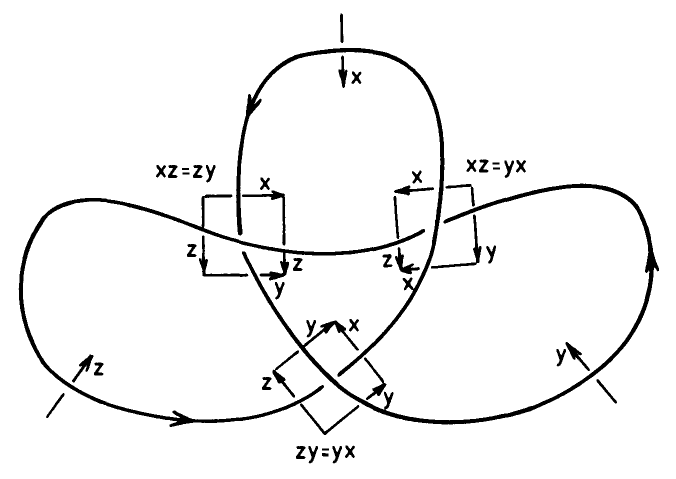
\includegraphics[width=12cm]{Images/gruponotrevo.png}
			\end{center}\caption{Cálculo do grupo de nó do nó de trevo.}
			\label{grupo no de trevo}
		\end{figure}
		\par\vspace{0.3cm} Usando a terminologia da figura, vemos que $\pi_1(\mathbb{R}^3\setminus K)$ é gerado por $3$ elementos $x, y, z$, sujeitos às relações $xz = zy, xz = yx$ e $zy = yx$. De acordo com o teorema de Wirtinger, qualquer uma dessas relações, digamos a terceira, pode ser omitida; isso pode ser verificado algebricamente: eliminando $z = x^{-1}yx$ da segunda relação, a primeira relação se torna $xyx = yxy$. Logo, obtemos uma apresentação para $\pi_1(\mathbb{R}^3\setminus K)$ do nó de trevo:
		\begin{align*}
		\pi_1(\mathbb{R}^3\setminus K) = \left< x,y \ | \ xyx = yxy \right>
		\end{align*}
		\par\vspace{0.3cm} Fazendo $a = xyx$ e $b = xy$, temos $x = b^{-1}a, y = a^{-1}b^2$ e $a^2 = (xyx)^2 = (xyx)(xyx) = (xyx)(yxy) = (xy)^3 = b^3$. Assim, podemos escrever o grupo do nó de trevo como
		\begin{align*}
		\pi_1(\mathbb{R}^3\setminus K) = \left< a,b \ | \ a^2 = b^3 \right>
		\end{align*}
		\par\vspace{0.3cm} Note que $\alpha = (12)$ e $\beta = (123)$ em $S_3$ também satisfazem $\alpha^2 = \beta^3 = e$. Logo, $S_3$ é imagem homomórfica de $\pi_1(\mathbb{R}^3\setminus K)$, o que implica que $\pi_1(\mathbb{R}^3\setminus K)$ não é abeliano. Em particular, o grupo de $K$ não é isomorfo ao grupo do nó trivial ($\mathbb{Z}$), logo $K$ não pode ser desatado sem cortes e colagens (como esperado).
	\end{example}
	\begin{example}[Nó figura oito]
		O nó figura oito é mostrado abaixo.
		\begin{figure}[H]
			\begin{center}
				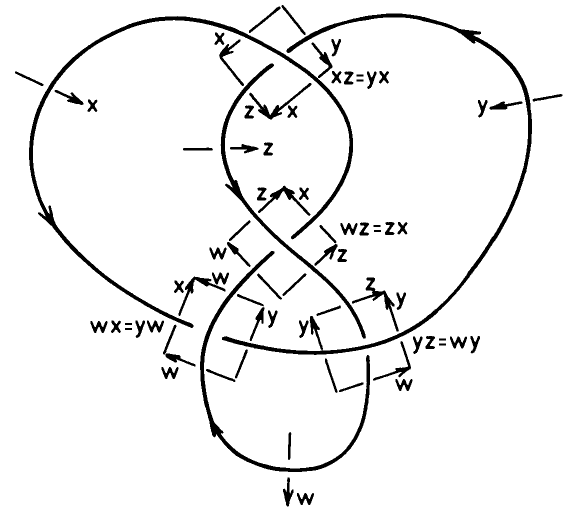
\includegraphics[width=10cm]{Images/gruponooito.png}
			\end{center}\caption{Cálculo do grupo de nó do nó figura oito}
			\label{grupo no de oito}	
		\end{figure}
		\par\vspace{0.3cm} O algoritmo de Wirtinger nos dá quatro geradores $x,y,z,w$ e quatro relações $xz = yx, wz = zx, yz = wy$ e $wx = yw$. Novamente, a última dessas relações pode ser omitida. Escrevemos a primeira relação na forma $z = x^{-1}yx$ e então a segunda relação na forma $w = zxz^{-1} = (x^{-1}yx)x(x^{-1}y^{-1}x) = x^{-1}yxy^{-1}x$; e a última relação, a terceira, torna-se $yx^{-1}yx = x^{-1}yxy^{-1}xy$. Logo, o grupo $\pi_1(\mathbb{R}^3\setminus K)$ do nó de trevo pode ser apresentado como
		\begin{align*}
		\pi_1(\mathbb{R}^3\setminus K) = \left< x,y \ | \ yx^{-1}yx = x^{-1}yxy^{-1}xy \right>
		\end{align*}
	\end{example}
	\par\vspace{0.3cm} Se dois nós têm grupos não isomorfos, então não é possível deformar um dos nós no outro; em particular, se o grupo de um nó não é isomorfo a $\mathbb{Z}$, então esse nó não é trivial. Portanto, podemos utilizar a teoria dos grupos para distinguir tipos diferentes de nós. Contudo, vale pontuar que se dois nós são dados por uma apresentação (como a apresentação de Wirtinger), em geral é um problema algébrico difícil decidir se esses grupos são isomorfos ou não.
	\par\vspace{0.3cm} Por outro lado, pode ser nos dado o problema puramente algébrico de decidir se dois grupos dados por apresentações são isomorfos ou não. Se soubermos que esses grupos ocorrem como grupos de nó, e também soubermos, por considerações topológicas, que esses nós não são equivalentes, então podemos concluir que esses dois grupos não são isomorfos. Portanto, não apenas a teoria dos grupos ajuda a topologia, mas reciprocamente!
	
	\section{Representação de Burau e os polinômios de Alexander e Jones} 
	\hspace{12pt} Como consequência do Teorema \eqref{teorema de Markov}, podemos usar tranças e a teoria das tranças para determinar invariantes de nós. Um dos exemplos mais elegantes desse método é o chamado \textit{polinômio de Alexander}, nomeado em homenagem ao matemático norte-americano J.W. Alexander, e denotado por $\Delta_K(t)$, sendo $K$ um nó (ou \textit{link}).
	\par\vspace{0.3cm} Mesmo com a descoberta do polinômio de Jones (outro invariante que também será tratado mais à frente) e seus híbridos em 1980, o polinômio de Alexander ainda permanece, mesmo após mais de 50 anos de pesquisa, um dos mais importantes e úteis invariantes de nós (e \textit{links}).
	\par\vspace{0.3cm} Para definir o polinômio de Alexander, devemos primeiro introduzir a chamada \textit{representação de Burau} de $B_n(\mathbb{R}^2)$. Então, seja $\beta\in B_n(\mathbb{R}^2)$. Podemos representar essa trança como
	\begin{align*}
	\beta = \sigma_{i_1}^{\varepsilon_1}\cdots\sigma_{i_k}^{\varepsilon_k}
	\end{align*}
	\par\vspace{0.3cm} com $1\leq i_1, \dots, i_k\leq n-1$ e $\varepsilon_i = \pm1$. Agora, vamos definir a função
	\begin{align*}
	\varphi_n: B_n\to M(n, \mathbb{Z}[t, t^{-1}])
	\end{align*}
	sendo $M(n, \mathbb{Z}[t,t^{-1}])$ as matrizes de ordem $n$ sobre o módulo $\mathbb{Z}[t,t^{-1}]$, tal que
	\begin{equation}
	\label{representacao de Burau}
	\varphi_n(\sigma_i) = 
	\left[ 
	\begin{array}{c|cc|c}
	I_{i-1} &  &  & \\
	\hline 
	& 1-t & t &  \\
	& 1 & 0 &  \\ 
	\hline
	&  &  & I_{n-i-1}
	\end{array}
	\right] 
	\end{equation}
	\par\vspace{0.3cm} sendo $I_m$ a matriz identidade de ordem $m$ e os espaços vazios correspondem a matrizes nulas. A representação de $B_n$ dada em \eqref{representacao de Burau} é chamada \textit{representação de Burau}. De fato, $\varphi_n$ é homomorfismo, como mostraremos a seguir.
	\begin{prop}
		\label{Burau e homomorfismo}
		A função $\varphi_n$ definida em \eqref{representacao de Burau} é homomorfismo. 
	\end{prop}
	\begin{proof}
		Basta mostrarmos que toda relação de $B_n$ é mapeada na matriz identidade ou, equivalentemente, que as relações de $B_n$ se mantêm para $\varphi_n$. 
		\par\vspace{0.3cm} Primeiro, vamos mostrar que se $|i - j|\geq 2$, então $\varphi_n(\sigma_i)\varphi_n(\sigma_j) = \varphi_n(\sigma_j)\varphi_n(\sigma_i)$. Sem perda de generalidade, podemos tomar $j>i+1$ e, portanto
		\begin{equation*}
		\varphi_n(\sigma_i)\varphi_n(\sigma_j) = 
		\left[ 
		\begin{array}{c|cc|c|cc|c}
		I_{i-1} & & & & & & \\
		\hline
		& 1-t & t & & & & \\
		& 1 & 0 & & & & \\
		\hline
		& & & I_{j-i-2} & & &\\
		\hline
		& & & & 1-t & t &\\
		& & & & 1 & 0 & \\
		\hline 
		& & & & & & I_{n-j-1} 
		\end{array}	
		\right] = \varphi_n(\sigma_j)\varphi_n(\sigma_i)
		\end{equation*}
		\par\vspace{0.3cm} sendo os espaços vazios preenchidos por matrizes nulas.
		\par\vspace{0.3cm} Agora, para a segunda e última relação, $\sigma_i\sigma_{i+1}\sigma_i = \sigma_{i+1}\sigma_i\sigma_{i+1}$, basta considerarmos o caso $n=3$, uma vez que na representação de Burau as entradas não nulas correspondem a matrizes identidade, ou seja, aumentando $n$ a partir de $3$, estaremos apenas acrescentando uma nova linha e uma nova coluna que serão ambas nulas com exceção da entrada diagonal, que será $1$; portanto, a multiplicação das matrizes não é afetada. 
		\par\vspace{0.3cm} Então, tomando $n = 3$, temos
		\begin{align*}
		\varphi_3(\sigma_1\sigma_2\sigma_1) &= \varphi_3(\sigma_1)\varphi_3(\sigma_2)\varphi_3(\sigma_1) \\ &= 
		\begin{bmatrix}
		1-t & t & 0 \\
		1 & 0 & 0 \\
		0 & 0 & 1
		\end{bmatrix}\begin{bmatrix}
		1 & 0 & 0 \\
		0 & 1-t & t \\
		0 & 1 & 0
		\end{bmatrix}\begin{bmatrix}
		1-t & t & 0 \\
		1 & 0 & 0 \\
		0 & 0 & 1
		\end{bmatrix} \\
		&= \begin{bmatrix}
		(1-t)^2 +t(1-t) & t(1-t) & t^2 \\
		1-t & t & 0 \\
		1 & 0 & 0
		\end{bmatrix} \\
		&= \begin{bmatrix}
		1 & 0 & 0 \\
		0 & 1-t & t \\
		0 & 1 & 0
		\end{bmatrix}\begin{bmatrix}
		1-t & t & 0 \\
		1 & 0 & 0 \\
		0 & 0 & 1
		\end{bmatrix}\begin{bmatrix}
		1 & 0 & 0 \\
		0 & 1-t & t \\
		0 & 1 & 0
		\end{bmatrix}\\
		&= \varphi_3(\sigma_2)\varphi_3(\sigma_1)\varphi_3(\sigma_2)\\
		&=\varphi_3(\sigma_2\sigma_1\sigma_2)
		\end{align*}
	\end{proof}
	\begin{remark}
		Em geral, a função $\varphi_n$ não é fiel, i.e., injetiva. Para $n=2$ e $n=3$, é sabido que $\varphi_n$ é fiel; para $n=4$, contudo, não sabemos.
	\end{remark}
	\par\vspace{0.3cm} Note também que como $\det(\varphi_n(\sigma_i)) = -t$ (basta expandir o determinante pelas primeiras $i-1$ linhas e, em seguida, pelas últimas $n-i-1$ linhas, restando apenas a matriz $\left[\begin{smallmatrix}
	1-t & t \\
	1 & 0
	\end{smallmatrix}\right]$), então existe o inverso de $\varphi_n(\sigma_i)$. Para computá-lo, note que
	\begin{align*}
	\varphi_n(1) = I_n = \varphi_n(\sigma_i\sigma_i^{-1}) = \varphi_n(\sigma_i)\varphi_n(\sigma_i^{-1}) \Leftrightarrow \varphi_n(\sigma_i^{-1}) = (\varphi_n(\sigma_i))^{-1}
	\end{align*} 
	\par\vspace{0.3cm} Calculando o inverso de $\varphi_n(\sigma_i)$ (que se resume basicamente a encontrar o inverso de $\left[\begin{smallmatrix}
	1-t & t\\
	1 & 0
	\end{smallmatrix}\right]$), obtemos
	\begin{align*}
	\varphi_n(\sigma_i^{-1}) = 
	\left[ 
	\begin{array}{c|cc|c}
	I_{i-1} &  &  & \\
	\hline 
	& 0 & 1 &  \\
	& t^{-1} & 1-t^{-1} &  \\ 
	\hline
	&  &  & I_{n-i-1}
	\end{array}
	\right] 
	\end{align*}
	\par\vspace{0.3cm} Por exemplo, tomando $\beta = \sigma_1\sigma_2^{-1}$, temos
	\begin{align*}
	\varphi_3(\beta) &= 
	\begin{bmatrix}
	1-t & t & 0 \\
	1 & 0 & 0 \\
	0 & 0 & 1
	\end{bmatrix}\begin{bmatrix}
	1 & 0 & 0 \\
	0 & 0 & 1 \\
	0 & t^{-1} & 1-t^{-1}
	\end{bmatrix}\\
	&= \begin{bmatrix}
	1-t & 0 & t \\
	1 & 0 & 0 \\
	0 & t^{-1} & 1-t^{-1}
	\end{bmatrix}
	\end{align*}
	\par\vspace{0.3cm} Vamos, agora, tratar do polinômio de Alexander em si.
	\par\vspace{0.3cm} Então, suponha que percebemos que uma quantidade $\lambda(\beta)$, derivada de uma trança $\beta$ de $n$ cordas, é um invariante de nó (ou \textit{link}). Devido ao Teorema \eqref{teorema de Markov}, para mostrar que $\lambda(\beta)$ é realmente um invariante, é suficiente mostrar que para uma trança $\beta$ de $n$ cordas valem as seguintes propriedades:
	\begin{enumerate}
		\item $\lambda(\beta) = \lambda(\gamma\beta\gamma^{-1})$ para $\gamma\in B_n$ arbitrária;
		\item $\lambda(\beta\sigma_n) = \lambda(\beta) = \lambda(\beta\sigma_n^{-1})$ para tranças de $n+1$ cordas $\beta\sigma_n$ e $\beta\sigma_n^{-1}$.
	\end{enumerate}
	\par\vspace{0.3cm} Voltando à representação de Burau apresentada anteriormente, uma quantidade que satisfaz as propriedades 1 e 2 é o determinante da matriz, pois como $\det(\varphi_n(\sigma_i)) = -t$, e sabendo que podemos escrever $\beta = \sigma_{i_1}^{\varepsilon_1}\cdots\sigma_{i_k}^{\varepsilon_k}$, temos
	\begin{align*} 
	\det(\varphi_n(\beta)) 
	&= 
	\det\left( \prod_{i=1}^{k}\varphi_n^{\varepsilon_i}(\sigma_i) \right)
	\\ 
	&= \prod_{i=1}^{k}(\det(\varphi_n(\sigma_i)))^{\varepsilon_i}
	\\ 
	&= (-t)^{\sum_{i=1}^{k}\varepsilon_i}
	\\
	&=(-t)^{l(\beta)} 
	\\
	&=(-t)^{l(\gamma\beta\gamma^{-1})} 
	\\
	&=\det(\varphi_n(\gamma\beta\gamma^{-1}))
	\end{align*} 
	\par\vspace{0.3cm} sendo $l$ a função homomorfismo de comprimento definida no Lema \eqref{homomorfismo de comprimento}. Em particular, note que
	\begin{equation}
	\label{det Burau de beta}
	\det(\varphi_n(\beta)) = (-t)^{l(\beta)}
	\end{equation}
	\par \vspace{0.3cm} Portanto, se fizermos $\lambda(\beta) = \det(\varphi_n(\beta))(-t)^{-\epsilon}$, sendo $\epsilon=l(\beta)$, então $\lambda(\beta)$ se torna um invariante. 
	\par\vspace{0.3cm} Contudo, esse invariante não é muito interessante, uma vez que $\lambda(\beta) = 1$ para toda trança $\beta$. Então, ao invés do determinante de $\varphi_n(\beta)$, vamos considerar o "polinômio característico" de $\varphi_n(\beta)$, a saber
	\begin{align*}
	\det(\varphi_n(\beta) - I_n)
	\end{align*}
	\par\vspace{0.3cm} Como veremos a seguir, isso leva a um invariante (não trivial) de nós, mas antes precisamos do seguinte lema técnico.
	\begin{lemma}
		\label{propriedades representacao de Burau}
		Escrevendo a representação de Burau de uma trança de $n$ cordas $\beta$ como $\varphi_n(\beta) = ||a_{ij}||$, $i,j=1,2,\dots,n$, então as seguintes propriedades valem:
		\begin{align}
		\label{propriedade 1}
		&\sum_{j=1}^{n}a_{ij} = 1 \\
		\label{propriedade 2}
		&\sum_{i=1}^{n} t^ia_{ij} = t^j 
		\end{align}
		\par Ou seja, a soma de todos os elementos da linha $i$ é igual a $1$ \eqref{propriedade 1} e somando os elementos da coluna $j$ (com o primeiro elemento multiplicado por $t$, o segundo por $t^2$ e assim por diante) obtemos $t^j$ \eqref{propriedade 2}.
	\end{lemma}
	\begin{proof}
		Primeiro, note que \eqref{propriedade 1} e \eqref{propriedade 2} valem se $\beta = \sigma_i^{\pm1}$, para $i$ qualquer, basta usar \eqref{representacao de Burau}. Agora, vamos mostrar que se $A$ e $B$ são duas matrizes que satisfazem \eqref{propriedade 1} e \eqref{propriedade 2}, então o seu produto $AB$ também satisfaz as mesmas equações. Mostrando isso, o resultado segue por indução.
		\par\vspace{0.3cm} Então, suponha $A = ||a_{ij}||$ e $B = || b_{kl} ||$ duas matrizes de ordem $n$ para as quais \eqref{propriedade 1} e \eqref{propriedade 2} valem. Além disso, seja $AB = || c_{pq} ||$, com $c_{pq} = \displaystyle{ \sum_{j=1}^{n}a_{pj}b_{jq} }$. Daí, 
		\begin{align*}
		&\sum_{q=1}^{n}c_{pq} = \sum_{q=1}^{n}\sum_{j=1}^{n}a_{pj}b_{jq} = \sum_{j=1}^{n}a_{pj}\underbrace{\left\{\sum_{q=1}^{n}b_{jq}\right\}}_{=1} =
		\sum_{j=1}^{n}a_{pj} = 1 \\
		&\sum_{p=1}^{n}t^pc_{pq} = \sum_{p=1}^{n}\sum_{j=1}^{n}t^pa_{pj}b_{jq} = \sum_{j=1}^{n}\underbrace{ \left\{ \sum_{p=1}^{n}t^pa_{pj} \right\}}_{=t^j}b_{jq} = \sum_{j=1}^{n}t^jb_{jq} = t^q
		\end{align*}	
	\end{proof}
	\par Segue imediatamente do Lema \eqref{propriedades representacao de Burau} que
	\begin{align}
	\label{consequencia 1}
	\sum_{j=1}^{n}(a_{ij} - \delta_{ij}) &= \sum_{j=1}^{n}a_{ij} - 1 = 0 \\ 
	\label{consequencia 2}
	\sum_{i=1}^{n}(t^ia_{ij} - t^i\delta_{ij}) &= \sum_{i=1}^{n}t^ia_{ij} - t^j = 0
	\end{align}
	\par sendo $\delta_{ij}$ o delta de Kronecker.
	\par\vspace{0.3cm} O significado da equação \eqref{consequencia 1} é que, na matriz $\varphi_n(\beta) - I_n$, excluindo a primeira coluna e adicionando todas as colunas restantes à primeira, obtemos uma coluna nula. Similarmente, na equação \eqref{consequencia 2} adicionamos a $i$-ésima linha multiplicada por $t^i$, $i=1,2,\dots,n$, à primeira linha, obtendo a linha nula. Consequentemente, obtemos
	\begin{equation*}
	\det(\varphi_n(\beta) - I_n) = 0
	\end{equation*}
	\par\vspace{0.3cm} Antes de seguir para o polinômio de Alexander em si, precisaremos dos dois lemas a seguir.
	\begin{lemma}
		\label{exercicio}
		Seja $M = \varphi_n(\beta)$ para uma trança $\beta$ de $n$ cordas. Denote por $M_{p,q}$ a matriz de ordem $(n-1)$ obtida de $M$ deletando a $p$-ésima linha e a $q$-ésima coluna, e denote o seu determinante por $\det[M]_{p,q}$. Então, valem as seguintes igualdades:
		\begin{enumerate}
			\item $\det[M - I_n]_{p,p} = t^{p-1}\det[M - I_n]_{1,1}$ para $p=1,2,\dots,n$
			\item $\det[M - I_n]_{p,q} = (-1)^{p+q}t^{p-1}\det[M - I_n]_{1,1}$ para quaisquer $1\leq p,q\leq n$.
		\end{enumerate}
	\end{lemma}
	\begin{proof}
		
	\end{proof}
	\par\vspace{0.3cm} Antes do próximo lema, convém fazer algumas definições. Então, seja $S$ uma matriz de ordem $n$ tal que
	\begin{align*}
	S &= \begin{bmatrix}
	1 & 1 & 1 & \cdots & 1 & 1 \\
	0 & 1 & 1 & \cdots & 1 & 1 \\
	0 & 0 & 1 & \cdots & 1 & 1 \\
	0 & 0 & 0 & \cdots & 1 & 1 \\
	\vdots & \vdots & \vdots & \ddots & \vdots & \vdots \\
	0 & 0 & 0 & \cdots & 1 & 1 \\
	0 & 0 & 0 & \cdots & 0 & 1
	\end{bmatrix}\\
	S^{-1} &= \begin{bmatrix}
	1 & -1 & 0 & \cdots & 0\\
	0 & 1  & -1 & \cdots & 0\\
	\vdots & \vdots & \ddots & \ddots & \vdots \\
	0 & 0 & \cdots & 1 & -1 \\
	0 & 0 & \cdots & 0 & 1
	\end{bmatrix}
	\end{align*}
	\par\vspace{0.3cm} Então, sendo $M = \varphi_n(\beta)$, temos
	\begin{equation*}
	S^{-1}MS = \left[\begin{array}{c|c}
	\Lambda(t) & \\
	\hline 
	\ast \cdots \ast & 1
	\end{array}\right] 
	\end{equation*}
	\par\vspace{0.3cm} em que $\Lambda(t)$ é uma matriz não singular $(n-1)\times(n-1)$. Portanto, temos $ \det[ S^{-1}MS - I_n]_{n,n} = \det[S^{-1}(M - I_n)S]_{n,n} = \det(\Lambda(t) - I_{n-1})$, uma vez que
	\begin{equation*}
	\det[S^{-1}(M - I_n)S]_{n,n} = \det[S^{-1}MS - I_n]_{n,n} = \det\Bigg[ \left[\begin{array}{c|c}
	\Lambda(t) - I_{n-1} & \\
	\hline
	\ast\cdots\ast & 0
	\end{array}\right]\Bigg]_{n,n} = \det(\Lambda(t) - I_{n-1}). 
	\end{equation*}
	\begin{lemma}
		\label{lema Alexander}
		Temos 
		\begin{align*}
		\det(\Lambda(t) - I_{n-1}) \doteq(1+t+\cdots+t^{n-1})\det[M-I_n]_{1,1}
		\end{align*}
		\par\vspace{0.3cm} ou, equivalentemente, 
		\begin{align*}
		\det[S^{-1}(M - I_{n})S]_{n,n} \doteq(1+t+\cdots+t^{n-1})\det[M-I_n]_{1,1}
		\end{align*}
		\par\vspace{0.3cm} em que $f\doteq g$ denota que $f = \pm t^kg$ para algum $k\in\mathbb{Z}$.
	\end{lemma}
	
	\begin{proof}
		Seja $M = ||a_{ij}||_{1\leq i,j\leq n}$. Por simplicidade, denote por $[M - I_n]_{0,n}$ a matriz $n\times(n-1)$ obtida deletando a $n$-ésima coluna. Então, as linhas de $[M - I_n]_{0,n}$ têm a seguinte forma:
		\begin{align*}
		A_1 =& \text{ }(a_{11} - 1, a_{12}, \dots, a_{1\text{ }n-1}) \\
		A_2 =& \text{ }(a_{21}, a_{22} - 1, \dots, a_{2\text{ }n-1}) \\
		\vdots& \\
		A_n =& \text{ }(a_{n1}, a_{n2}, \dots, a_{n\text{ }n-1})
		\end{align*}
		\par\vspace{0.3cm} Uma computação direta e cuidadosa nos dá
		\begin{equation*}
		U(\Lambda(t) - I_{n-1})V = \begin{bmatrix}
		A_1 - A_2 \\
		A_1 - A_3 \\
		\vdots \\
		A_1 - A_n
		\end{bmatrix}
		\end{equation*}
		\par\vspace{0.3cm} sendo $U = [S^T]_{n,n}$ e $V = [S^{-1}]_{n,n}$. Daí, usando a multilinearidade do determinante, obtemos:
		\begin{align*}
		\det(\Lambda(t) - I_{n-1}) 
		&=\det[U(\Lambda(t) - I_{n-1})V] 
		\\
		&= \det\begin{bmatrix}
		A_1 - A_2\\
		A_1 - A_3 \\
		\vdots \\
		A_1 - A_n
		\end{bmatrix}
		\\
		&= \det\begin{bmatrix}
		A_1 \\
		-A_3 \\
		-A_4 \\
		\vdots \\
		-A_n
		\end{bmatrix} + \det\begin{bmatrix}
		-A_2 \\
		A_1 \\
		-A_4 \\
		\vdots\\
		-A_n
		\end{bmatrix} +\cdots + \det\begin{bmatrix}
		-A_2 \\
		\vdots\\
		-A_k \\
		A_1\\
		-A_{k+2}\\
		\vdots\\
		-A_n
		\end{bmatrix} +\cdots + 
		\det\begin{bmatrix}
		-A_2\\
		-A_3 \\
		\vdots\\
		-A_{n-1}\\
		A_1
		\end{bmatrix}+\det\begin{bmatrix}
		-A_2\\
		-A_3\\
		\vdots\\
		-A_n
		\end{bmatrix}
		\end{align*}
		\par\vspace{0.3cm} Daí, temos
		\begin{align*}
		\det\begin{bmatrix}
		-A_2\\
		-A_3\\
		\vdots \\
		-A_n
		\end{bmatrix} = (-1)^{n-1}\det[M-I_n]_{1,n} = (-1)^{n-1+n+1}t^0\det[M - I_n]_{1,1} = \det[M-I_n]_{1,1}
		\end{align*}
		\par\vspace{0.3cm} em que na primeira igualdade retiramos todos os fatores $-1$ do determinante e, na segunda igualdade, utilizamos o Lema \eqref{exercicio}. Analogamente, temos
		\begin{align*}
		\det\begin{bmatrix}
		A_1\\
		-A_3\\
		\vdots\\
		-A_n
		\end{bmatrix} = (-1)^{n-2}\det[M-I_n]_{2,n} = (-1)^{n-2+n+2}t^1\det[M - I_n]_{1,1} = t\det[M - I_n]_{1,1}
		\end{align*}
		\par\vspace{0.3cm} Por fim, de modo análogo para todo $2\leq k\leq n-1$, obtemos
		\begin{equation*}
		\det\begin{bmatrix}
		-A_2 \\
		\vdots\\
		-A_k\\
		A_1\\
		-A_{k+2}\\
		\vdots\\
		-A_n
		\end{bmatrix} = (-1)^{n-2+k-1}\det\begin{bmatrix}
		A_1\\
		A_2\\
		\vdots\\
		A_k\\
		A_{k+2}\\
		\vdots\\
		A_n
		\end{bmatrix} = (-1)^{n+k-3}\det[M - I_n]_{k+1, n} = t^k\det[M - I_n]_{1,1}
		\end{equation*}
		\par\vspace{0.3cm} Consequentemente, $\det(\Lambda(t) - I_{n-1}) = (1+t+\cdots+t^{n-1})\det[M - I_n]_{1,1}$	
	\end{proof}
	\par\vspace{0.3cm} Agora estamos prontos para enunciar e demonstrar o teorema desejado.
	\begin{theorem}
		\label{polinomio de Alexander}
		Seja $K$ um nó (ou link) orientado e suponha $\beta$ uma trança de $n$ cordas cujo fecho é $K$. Se fizermos $M = \varphi_n(\beta)$, então $\det[M - I_n]_{1,1}$ é um invariante de $K$, a menos de um fator $\pm t^k$, para algum $k\in\mathbb{Z}$.
	\end{theorem} 
	\par\vspace{0.3cm} A essência do Teorema \eqref{polinomio de Alexander} é que se $\beta_1\in B_n$ e $\beta_2\in B_m$ são duas tranças cujos fechos são equivalentes, i.e., tais que $\widetilde{\beta_1}\approx\widetilde{\beta_2}$, então existe $k\in\mathbb{Z}$ tal que
	\begin{equation*}
	\det[\varphi_n(\beta_1) - I_n]_{1,1}=\pm t^k\det[\varphi_m(\beta_2) - I_m]_{1,1}
	\end{equation*}
	\par\vspace{0.3cm} Esse invariante é chamado \textit{polinômio de Alexander} (reduzido) de $K$ e denotado por $\Delta_K(t)$. Multiplicando por um fator adequado, $\Delta_K(t)$ (se não for nulo) pode ser escrito como
	\begin{equation*}
	\Delta_K(t) = c_0 + c_1t + \cdots + c_mt^m, c_0>0
	\end{equation*}
	\par\vspace{0.3cm} Agora, para a demonstração.
	\begin{proof}
		Pelo Teorema \eqref{teorema de Markov}, basta mostrarmos que para duas tranças quaisquer $\beta$ e $\gamma$ de $n$ cordas, valem
		\begin{enumerate}
			\item $\det[\varphi_n(\gamma\beta\gamma^{-1}) - I_n]_{1,1} \doteq \det[\varphi_n(\beta) - I_n]_{1,1}$
			\item $\det[\varphi_n(\beta\sigma_n) - I_{n+1}]_{1,1}\doteq\det[\varphi_n(\beta) - I_n]_{1,1} \doteq \det[\varphi_n(\beta\sigma_n^{-1}) - I_{n+1}]_{1,1}$
		\end{enumerate}
		\par\vspace{0.3cm} Note que em 2, o centro é o determinante de uma matriz de ordem $n-1$, enquanto que nos lados esquerdo e direito temos o determinante de uma matrix de ordem $n$. Vamos começar com a demonstração de 1.
		\par\vspace{0.3cm} Suponha $\beta$ e $\gamma$ duas tranças de $n$ cordas. Então, podemos escrever
		\begin{equation*}
		S^{-1}\varphi_n(\beta)S = \left[ \begin{array}{c|c}
		\Lambda(\beta) & \\
		\hline
		a_1\cdots a_{n-1} & 1
		\end{array}\right] \text{ e } 
		S^{-1}\varphi_n(\gamma)S = \left[  \begin{array}{c|c}
		\Lambda(\gamma) & \\
		\hline 
		b_1 \cdots b_{n-1} & 1
		\end{array}\right]  
		\end{equation*}
		\par\vspace{0.3cm} Similarmente, podemos escrever
		\begin{equation*}
		S^{-1}\varphi_n(\gamma^{-1})S = \left[\begin{array}{c|c}
		\Lambda^{-1}(\gamma) & \\
		\hline 
		c_1\cdots c_{n-1} & 1
		\end{array}\right]
		\end{equation*}
		\par\vspace{0.3cm} Logo, multiplicando essas matrizes e usando o fato de que $\varphi_n$ é homomorfismo, temos
		\begin{equation*}
		S^{-1}\varphi_n(\gamma\beta\gamma^{-1})S = \left[\begin{array}{c|c}
		\Lambda(\gamma)\Lambda(\beta)\Lambda^{-1}(\gamma) & \\
		\hline 
		d_1\cdots d_{n-1} & 1
		\end{array}\right]
		\end{equation*}
		\par\vspace{0.3cm} e, portanto, 
		\begin{align*}
		\det[S^{-1}\varphi_n(\gamma\beta\gamma^{-1})S - I_n]_{n,n} &= \det(\Lambda(\gamma)\Lambda(\beta)\Lambda^{-1}(\gamma) - I_{n-1}) \\ 
		&= \det[\Lambda(\gamma)(\Lambda(\beta) - I_{n-1})\Lambda^{-1}(\gamma)] \\
		&= \det(\Lambda(\gamma))\det(\Lambda^{-1}(\gamma))\det(\Lambda(\beta) - I_{n-1}) \\
		&= \det(\Lambda(\beta) - I_{n-1})
		\end{align*}
		\par\vspace{0.3cm} Aplicando o Lema \eqref{lema Alexander} a ambos os lados da igualdade, temos
		\begin{align*}
		(1 + t + \cdots + t^{n-1})\det[\varphi_n(\gamma\beta\gamma^{-1}) - I_n]_{1,1}\doteq(1+t+\cdots+t^{n-1})\det[\varphi_n(\beta) - I_n]_{1,1}
		\end{align*}
		\par\vspace{0.3cm} e, portanto, 
		\begin{equation*}
		\det[\varphi_n(\gamma\beta\gamma^{-1}) - I_n]_{1,1}\doteq\det[\varphi_n(\beta) - I_n]_{1,1}
		\end{equation*}
		\par\vspace{0.3cm} finalizando a demonstração de 1. Agora, para a demonstração de 2.
		\par\vspace{0.3cm} Suponha $\beta$ uma trança de $n$ cordas e seja $\varphi_n(\beta)(=M) = ||a_{ij}||$. Se considerarmos $\beta\in B_{n+1}$, então
		\begin{equation*}
		\varphi_{n+1}(\beta) = \left[\begin{array}{c|c}
		M & \\
		\hline
		& 1
		\end{array}\right]
		\end{equation*}
		\par\vspace{0.3cm} e, como da definição da representação de Burau em \eqref{representacao de Burau}, temos
		\begin{equation*}
		\varphi_{n+1}(\sigma_n) = \left[\begin{array}{c|cc}
		I_{n-1} & & \\
		\hline
		& 1-t & t \\
		& 1 & 0
		\end{array}\right]
		\end{equation*}
		\par\vspace{0.3cm} Multiplicando as duas matrizes acima e usando o fato de que $\varphi_n$  é homomorfismo, segue que
		\begin{equation*}
		\varphi_{n+1}(\beta\sigma_n) = \left[\begin{array}{c|cc}
		& a_{1n}(1-t) & a_{1n}t \\
		M_{n,n} & \vdots & \vdots \\
		& a_{n-1\text{ }n}(1-t) & a_{n-1\text{ }n}t \\
		a_{n1}\cdots a_{n\text{ }n-1} & a_{n\text{ }n}(1-t) & a_{n\text{ }n}t \\
		\hline 
		& 1 & 0
		\end{array}\right]
		\end{equation*}
		\par\vspace{0.3cm} Logo,
		\begin{align*}
		\det[\varphi_{n+1}(\beta\sigma_n) - I_{n+1}]_{n,n} &= \det\left[\begin{array}{c|c}
		& a_{1n}t \\
		M_{n,n} - I_{n-1} & \vdots \\
		& a_{n-1\text{ }n}t \\
		\hline
		& -1
		\end{array}\right] \\
		&= -\det[M_{n,n} - I_{n-1}] \\
		&= -\det[\varphi_n(\beta) - I_n]_{n,n} \\
		&\doteq \det[\varphi_n(\beta) - I_n]_{n,n} 
		\end{align*} 
		\par\vspace{0.3cm} Pelo Lema \eqref{exercicio}, sabemos que $\det[M-I_n]_{1,1}\doteq\det[M-I_n]_{n,n}$. Daí, aplicando esse fato a ambos os lados da igualdade, obtemos
		\begin{equation*}
		\det[\varphi_{n+1}(\beta\sigma_n) - I_{n+1}]_{1,1}\doteq\det[\varphi_{n+1}(\beta\sigma_n) - I_{n+1}]_{n,n}\doteq\det[\varphi_n(\beta) - I_n]_{1,1}
		\end{equation*}
		\par\vspace{0.3cm} De modo similar, podemos escrever
		\begin{equation*}
		\varphi_{n+1}(\sigma_n^{-1}) = \left[\begin{array}{c|cc}
		I_{n-1} & & \\
		\hline
		& 0 & 1 \\
		& t^{-1} & 1-t^{-1}
		\end{array}\right]
		\end{equation*}
		\par\vspace{0.3cm} Daí, novamente usando a definição da representação de Burau em \eqref{representacao de Burau}, temos
		\begin{equation*}
		\varphi_{n+1}(\beta\sigma_n^{-1}) = \left[\begin{array}{c|c|c}
		&  & a_{1n} \\
		M_{n,n} &  & \vdots \\
		&  & a_{n-1\text{ }n} \\
		a_{n1}\cdots a_{n\text{ }n-1} &  & a_{n\text{ }n} \\
		\hline 
		& t^{-1} & 1-t^{-1}
		\end{array}\right]
		\end{equation*}
		\par\vspace{0.3cm} Logo, multiplicando as matrizes acima e usando o fato de que $\varphi_n$ é homomorfismo, segue que
		\begin{align*}
		\det[\varphi_{n+1}(\beta\sigma_n^{-1}) - I_{n+1}]_{n,n} &= \det\left[\begin{array}{c|c}
		& a_{1n} \\
		M_{n,n} - I_{n-1} &  \vdots \\
		& a_{n-1\text{ }n} \\
		\hline
		& -t^{-1}
		\end{array}\right] \\
		&= -t^{-1}\det[M_{n,n} - I_{n-1}] \\
		&= -t^{-1}\det[\varphi_n(\beta) - I_n]_{n,n} \\
		&\doteq \det[ \varphi_n(\beta) - I_n]_{n,n}
		\end{align*} 
		\par\vspace{0.3cm} Pelo Lema \eqref{exercicio}, sabemos que $\det[M-I_n]_{1,1}\doteq\det[M-I_n]_{n,n}$. Daí, aplicando esse fato a ambos os lados da igualdade, obtemos
		\begin{equation*}
		\det[\varphi_{n+1}(\beta\sigma_n^{-1}) - I_{n+1}]_{1,1}\doteq\det[\varphi_{n+1}(\beta\sigma_n^{-1}) - I_{n+1}]_{n,n}\doteq\det[\varphi_n(\beta) - I_n]_{1,1}
		\end{equation*}
		\par\vspace{0.3cm} e concluímos a demonstração.	
	\end{proof}
	\par\vspace{0.3cm} Por exemplo, o nó trivial em $B_1$ é $\beta = 1$. Logo, $\varphi_1(1) = [1]$ e então $\varphi_1(1) - 1 = [0]$ e $[\varphi_1(1) - 1]_{1,1}$ é a matriz vazia, $\emptyset$. Vamos definir $\det(\emptyset) = 1$, e então $\Delta_{\widetilde{1}}(t) = 1$. 
	\par\vspace{0.3cm} O nó trivial também é representado por $\sigma_1$ em $B_2$. Nesse caso, 
	\begin{equation*}
	N = \varphi_2(\sigma_1) - I_2 = \begin{bmatrix}
	-t & t \\
	1 & -1
	\end{bmatrix}
	\end{equation*}
	\par\vspace{0.3cm} logo, $\det[N]_{1,1} = -1$ e $\det[N]_{2,2} = -t$ e temos, novamente, $\Delta_{\widetilde{\sigma}_1}(t) = 1$.
	\par\vspace{0.3cm} Por outro lado, em $B_3$ a trança $\sigma_1$ representa o fecho de um \textit{link} trivial de 2 componentes. Nesse caso, 
	\begin{equation*}
	N = \varphi_3(\sigma_1) - I_3 = \begin{bmatrix}
	-t & t & 0 \\
	1 & -1 & 0 \\
	0 & 0 & 0
	\end{bmatrix}
	\end{equation*}
	\par\vspace{0.3cm} e, portanto, $\det[N]_{1,1} = 0$. Logo, para $\sigma_1\in B_3$, $\Delta_{\widetilde{\sigma}_1}(t) = 0$. Note que acabamos de mostrar que o polinômio de Alexander pode ser $0$ para um \textit{link}.
	\par\vspace{0.3cm} Tomando $\beta = \sigma_1\sigma_2$ em $B_3$, temos que $\widetilde{\beta}$, i.e, o fecho de $\beta$, é o nó trivial. Nesse caso, temos
	\begin{equation*}
	\varphi_3(\beta) - I_3 = \begin{bmatrix}
	-t & t(1-t) & t^2 \\
	1 & -1 & 0 \\
	0 & 1 & -1
	\end{bmatrix}
	\end{equation*}
	\par\vspace{0.3cm} logo, $\det[\varphi_3(\beta)-I_3]_{1,1} = 1 = \Delta_{\widetilde{\beta}}(t)$, como esperado.
	\par\vspace{0.3cm} Da Figura \eqref{exemplo invariante de Alexander}, pode-se mostrar que $\beta_1\underset{M}{\sim}\beta_2$. Vamos ver o que acontece quando calculamos $\varphi_3(\beta_1)$ e $\varphi_2(\beta_2)$ (esperamos que sejam iguais).
	\begin{figure}[H]
		\begin{center}
			\includegraphics[width=9cm]{Images/exemplo_invariante_alexander.png}
		\end{center}\caption{Dois nós Markov equivalentes.}\label{exemplo invariante de Alexander}
	\end{figure}
	\par\vspace{0.3cm} Como $\beta_1 = (\sigma_1\sigma_2)^2$ e $\beta_2 = \sigma_1^3$ e, por definição, 
	\begin{equation*}
	\varphi_3(\sigma_1) = \begin{bmatrix}
	1-t & t & 0 \\
	1 & 0 & 0 \\
	0 & 0 & 1 
	\end{bmatrix}\text{ e } \varphi_3(\sigma_2) = \begin{bmatrix}
	1 & 0 & 0 \\
	0 & 1-t & t \\
	0 & 1 & 0
	\end{bmatrix}
	\end{equation*}
	\par\vspace{0.3cm} segue que
	\begin{equation*}
	\varphi_3(\sigma_1\sigma_2)^2 = \begin{bmatrix}
	1-t & t-t^2+t^3 & t^2-t^3 \\
	1-t & t-t^2 & t^2 \\
	1 & 0 & 0
	\end{bmatrix}
	\end{equation*}
	\par\vspace{0.3cm} Logo, 
	\begin{equation*}
	\Delta_{\widetilde{\beta}_1}(t) = \det[\varphi_3(\beta_1) - I_3]_{1,1} = \det\begin{bmatrix}
	-1+t-t^2 & t^2 \\
	0 & -1
	\end{bmatrix} = 1-t+t^2
	\end{equation*}
	\par\vspace{0.3cm} Por outro lado, 
	\begin{equation*}
	\varphi_2(\sigma_1) = \begin{bmatrix}
	1-t & t \\
	1 & 0
	\end{bmatrix}\text{ e }\varphi_2(\sigma_1)^3 = \begin{bmatrix}
	1-t+t^2-t^3 & t(1-t+t^2) \\
	1-t+t^2 & t-t^2
	\end{bmatrix}
	\end{equation*}
	\par\vspace{0.3cm} Logo, 
	\begin{equation*}
	\Delta_{\widetilde{\beta}_2}(t) = \det[\varphi_2(\beta_2) - I_2]_{1,1} = -1+t-t^2
	\end{equation*}
	\par\vspace{0.3cm} e, consequentemente, $\Delta_{\widetilde{\beta}_1}(t) = -\Delta_{\widetilde{\beta}_2}(t)$, ou seja, 
	\begin{equation*}
	\Delta_{\widetilde{\beta}_1}(t)\doteq\Delta_{\widetilde{\beta}_2}(t)
	\end{equation*}
	\par\vspace{0.3cm} como esperado.
	\par\vspace{0.3cm} Observe os nós da Figura \eqref{nos exemplo polinomio Alexander}. O nó (a) é o nó $K_a$, fecho de $(\sigma_1\sigma_2^{-1})^2$ em $B_3$ e o nó (b) é o nó $K_b$, fecho de $\sigma_1^n$ em $B_2$.
	\begin{figure}[H]
		\begin{center}
			\includegraphics[width=9cm]{Images/no_de_oito_Alexander.png}
		\end{center}\caption{O nó figura oito (a) e um nó com $n$ cruzamentos (b).}\label{nos exemplo polinomio Alexander}
	\end{figure}
	\par\vspace{0.3cm} Por definição, temos
	\begin{equation*}
	\varphi_3(\sigma_1\sigma_2^{-1}) = \begin{bmatrix}
	1-t & t & 0 \\
	1 & 0 & 0 \\
	0 & 0 & 1
	\end{bmatrix}\begin{bmatrix}
	1 & 0 & 0 \\
	0 & 0 & 1 \\
	0 & t^{-1} & 1-t^{-1}
	\end{bmatrix} = \begin{bmatrix}
	1-t & 0 & t \\
	1 & 0 & 0 \\
	0 & t^{-1} & 1-t^{-1}
	\end{bmatrix}
	\end{equation*}
	\par\vspace{0.3cm} Logo,
	\begin{equation*}
	\varphi_3(\sigma_1\sigma_2^{-1})^2 = \begin{bmatrix}
	1-t & 0 & t \\
	1 & 0 & 0 \\
	0 & t^{-1} & 1-t^{-1}
	\end{bmatrix}\begin{bmatrix}
	1-t & 0 & t \\
	1 & 0 & 0 \\
	0 & t^{-1} & 1-t^{-1}
	\end{bmatrix} = \begin{bmatrix}
	(1-t)^2 & 1 & -1 +2t-t^2 \\
	1-t & 0 & t \\
	t^{-1} & t^{-1}-t^{-2} & (1-t^{-1})^2
	\end{bmatrix}
	\end{equation*}
	\par\vspace{0.3cm} Daí, obtemos
	\begin{equation*}
	\Delta_{K_a}(t) = \det[\varphi_3(\sigma_1\sigma_2^{-1})^2 - I_3]_{1,1} = \det\begin{bmatrix}
	-1 & t \\
	t^{-1} - t^{-2} & -1+(1-t^{-1})^2
	\end{bmatrix} = -1+3t^{-1}-t^{-2} \underset{\times (-t^2)}{\doteq} 1-3t+t^2
	\end{equation*}
	\par\vspace{0.3cm} Para o nó $K_b$, temos que
	\begin{equation*}
	\varphi_2(\sigma_1)^n = \begin{bmatrix}
	1-t & t \\
	1 & 0
	\end{bmatrix}^n
	\end{equation*}
	\par\vspace{0.3cm} Como $\varphi_2(\sigma_1)$ tem autovalores $\lambda_{1,2} = 1, -t$ e autovetores $v_{1,2} = (1,1), (-t,1)$, obtemos
	\begin{align*}
	\varphi_2(\sigma_1)^n &= \frac{1}{1+t}\begin{bmatrix}
	1 & -t \\
	1 & 1
	\end{bmatrix}\begin{bmatrix}
	1 & 0 \\
	0 & -t
	\end{bmatrix}^n\begin{bmatrix}
	1 & t \\
	-1 & 1
	\end{bmatrix} \\
	&= \frac{1}{1+t}\begin{bmatrix}
	1 & -t \\
	1 & 1
	\end{bmatrix}\begin{bmatrix}
	1 & 0 \\
	0 & (-t)^n
	\end{bmatrix}\begin{bmatrix}
	1 & t \\
	-1 & 1
	\end{bmatrix} \\
	&= \frac{1}{1+t}\begin{bmatrix}
	1 & (-t)^{n+1} \\
	1 & (-t)^n
	\end{bmatrix}\begin{bmatrix}
	1 & t \\
	-1 & 1
	\end{bmatrix} \\
	&= \frac{1}{1+t}\begin{bmatrix}
	1 - (-t)^{n+1} & t + (-t)^{n+1} \\
	1 - (-t)^n & t + (-t)^n
	\end{bmatrix}
	\end{align*}
	\par\vspace{0.3cm} Daí, temos que
	\begin{align*}
	\Delta_{K_b}(t) = \det[\varphi_2(\sigma_1)^n - I_2]_{1,1} &= \frac{1}{1+t}[t+(-t)^n] - 1 \\
	&= \frac{-1 + (-t)^n}{1+t} \\
	&= -\frac{1 - (-t)^n}{1+t} \\
	&= -\sum_{i=1}^{n}(-t)^{i-1} \\
	&= -(1-t+t^2-\cdots+(-1)^{n-1}t^{n-1}) \\
	&\doteq 1-t+t^2-\cdots+(-1)^{n-1}t^{n-1} 
	\end{align*}
	\par\vspace{0.3cm} Em particular, para $n = 3$ temos o nó de trevo (veja Figura \eqref{no de trevo}) e o polinômio de Alexander $\Delta_{K_b} = 1-t+t^2\underset{\times(t^{-1})}{\doteq} t-1+t^{-1}$.
	\par\vspace{0.3cm} Outro exemplo interessante é o nó toral $K_{a,b}$, cujo polinômio de Alexander é
	\begin{equation*}
	\Delta_{K_{a,b}} = \frac{(1-t^{ab})(1-t)}{(1-t^a)(1-t^b)}
	\end{equation*}
	\par\vspace{0.3cm} Usando a representação de Burau $\varphi_n: B_n\to M(n, \mathbb{Z}[t,t^{-1}])$, podemos definir outras funções. Por exemplo, podemos definir $\overline{\varphi}_n: B_n\to M(n-1, \mathbb{Z}[t,t^{-1}])$ dada por
	\begin{equation*}
	\overline{\varphi}_n(\beta) = \Lambda(t)
	\end{equation*} 
	\par\vspace{0.3cm} sendo $\Lambda(t)$ a matriz definida logo antes do Lema \eqref{lema Alexander}. Daí, afirmamos o seguinte.
	\begin{prop}
		\label{parecido com Burau}
		A função $\overline{\varphi}_n$ é um homomorfismo. %Além disso, para quaisquer $\beta, \gamma\in B_n$, valem as igualdades:
		%\begin{enumerate}
		%\item $\overline{\varphi}_n(\gamma\beta\gamma^{-1}) = %\overline{\varphi}_n(\beta)$
		%\item %$\overline{\varphi}_{n+1}(\beta\sigma_n)(1+t+\cdots+t^%{n-1}) = \overline{\varphi}_n(\beta)(1+t+\cdots+t^n)$
		%\end{enumerate}
	\end{prop}
	\begin{proof}
		Vamos mostrar que $\overline{\varphi}_n$ é homomorfismo. Primeiro, note que se $|i-j|\geq 2$, temos
		\begin{align*}
		(S^{-1}\varphi_n(\sigma_i)S)(S^{-1}\varphi_n(\sigma_j)S) &= S^{-1}\varphi_n(\sigma_i)\varphi_n(\sigma_j)S \\ 
		&= S^{-1}\varphi_n(\sigma_j)\varphi_n(\sigma_i)S \\
		&= (S^{-1}\varphi_n(\sigma_j)S)(S^{-1}\varphi_n(\sigma_i)S)
		\end{align*}
		\par\vspace{0.3cm} Isso implica que
		\begin{align*}
		\left[ \begin{array}{c|c}
		\Lambda(\sigma_i)\Lambda(\sigma_j) & \\
		\hline
		\ast\cdots\ast & 1
		\end{array}\right] = 
		\left[ \begin{array}{c|c}
		\Lambda(\sigma_i) & \\
		\hline
		\ast\cdots\ast & 1
		\end{array}\right]\left[ \begin{array}{c|c}
		\Lambda(\sigma_j) & \\
		\hline
		\ast\cdots\ast & 1
		\end{array}\right]  = \left[\begin{array}{c|c}
		\Lambda(\sigma_j) & \\
		\hline
		\ast\cdots\ast & 1
		\end{array}\right]\left[ \begin{array}{c|c}
		\Lambda(\sigma_i) & \\
		\hline
		\ast\cdots\ast & 1
		\end{array}\right] =  \left[\begin{array}{c|c}
		\Lambda(\sigma_j)\Lambda(\sigma_i) & \\
		\hline
		\ast\cdots\ast & 1
		\end{array}\right]
		\end{align*}
		\par\vspace{0.3cm} ou seja, $\overline{\varphi}_n(\sigma_i)\overline{\varphi}_n(\sigma_j) = \overline{\varphi}_n(\sigma_j)\overline{\varphi}_n(\sigma_i)$ para $|i-j|\geq 2$.
		\par\vspace{0.3cm} De modo similar, vamos mostrar que $\overline{\varphi}_n(\sigma_i)\overline{\varphi}_n(\sigma_{i+1})\overline{\varphi}_n(\sigma_i) = \overline{\varphi}_n(\sigma_{i+1})\overline{\varphi}_n(\sigma_i)\overline{\varphi}_n(\sigma_{i+1})$, ou seja, que $\Lambda(\sigma_i)\Lambda(\sigma_{i+1})\Lambda(\sigma_i) = \Lambda(\sigma_{i+1})\Lambda(\sigma_i)\Lambda(\sigma_{i+1})$. Para isso, basta considerar o caso para $n=3$ pelo mesmo motivo que o fizemos na demonstração da Proposição \eqref{Burau e homomorfismo}. Note que
		\begin{align*}
		(S^{-1}\varphi_3(\sigma_1)S)(S^{-1}\varphi_3(\sigma_2)S)(S^{-1}\varphi_3(\sigma_1)S) = (S^{-1}\varphi_3(\sigma_2)S)(S^{-1}\varphi_3(\sigma_1)S)(S^{-1}\varphi_3(\sigma_2)S)
		\end{align*}
		\par\vspace{0.3cm} Isso implica que 
		\begin{align*}
		\left[\begin{array}{c|c}
		\Lambda(\sigma_1)\Lambda(\sigma_2)\Lambda(\sigma_1) & \\
		\hline 
		\ast\cdots\ast & 1
		\end{array}\right] &= \left[\begin{array}{c|c}
		\Lambda(\sigma_1) & \\
		\hline
		\ast\cdots\ast & 1
		\end{array}\right]\left[\begin{array}{c|c}
		\Lambda(\sigma_2) & \\
		\hline
		\ast\cdots\ast & 1
		\end{array}\right]\left[\begin{array}{c|c}
		\Lambda(\sigma_1) & \\
		\hline
		\ast\cdots\ast & 1
		\end{array}\right] \\ 
		&= \left[\begin{array}{c|c}
		\Lambda(\sigma_2) & \\
		\hline
		\ast\cdots\ast & 1
		\end{array}\right]\left[\begin{array}{c|c}
		\Lambda(\sigma_1) & \\
		\hline
		\ast\cdots\ast & 1
		\end{array}\right]\left[\begin{array}{c|c}
		\Lambda(\sigma_2) & \\
		\hline
		\ast\cdots\ast & 1
		\end{array}\right] \\
		&= \left[\begin{array}{c|c}
		\Lambda(\sigma_2)\Lambda(\sigma_1)\Lambda(\sigma_2) & \\
		\hline
		\ast\cdots\ast & 1
		\end{array}\right]
		\end{align*}
		\par\vspace{0.3cm} como queríamos mostrar. Portanto, $\overline{\varphi}_n$ de fato é homomorfismo.
	\end{proof}
	\par\vspace{0.3cm} Também é possível mostrar que para quaisquer $\beta, \gamma\in B_n$, valem as igualdades:
	\begin{enumerate}
		\item $\overline{\varphi}_n(\gamma\beta\gamma^{-1}) = \overline{\varphi}_n(\beta)$
		\item $\overline{\varphi}_{n+1}(\beta\sigma_n)(1+t+\cdots+t^{n-1}) = \overline{\varphi}_n(\beta)(1+t+\cdots+t^n)$
	\end{enumerate}
	\par\vspace{0.3cm} Desse modo, vamos definir, para uma trança $\beta\in B_n$ arbitrária, 
	\begin{equation*}
	\lambda(\beta) = \frac{\overline{\varphi}_n(\beta)}{1+t+\cdots+t^{n-1}}
	\end{equation*} 
	\par\vspace{0.3cm} Então, $\lambda(\beta)$ é um invariante do fecho de $\beta$, ou seja, se os fechos de $\beta_1\in B_n$ e $\beta_2\in B_m$ representam o mesmo nó $K$, então
	\begin{equation*}
	\frac{\overline{\varphi}_n(\beta_1)}{1+t+\cdots+t^{n-1}} = \frac{\overline{\varphi}_m(\beta_2)}{1+t+\cdots+t^{m-1}}
	\end{equation*}
	\par\vspace{0.3cm} Pode ser mostrado que, na verdade, $\overline{\varphi}_n(\beta)$ é o polinômio de Alexander de $\widetilde{\beta}$.
	\par\vspace{0.3cm} Podemos definir também $\varphi_n^\ast: B_n\to M(n, \mathbb{Z}[t,t^{-1}])$ por
	\begin{equation*}
	\varphi_n^\ast(\sigma_{i_1}^{\varepsilon_1}\sigma_{i_2}^{\varepsilon_2}\cdots\sigma_{i_k}^{\varepsilon_k}) = \varphi_n(\sigma_{i_1}^{\varepsilon_1})^T\varphi_n(\sigma_{i_2}^{\varepsilon_2})^T\cdots\varphi_n(\sigma_{i_k}^{\varepsilon_k})^T
	\end{equation*}
	\par\vspace{0.3cm} De fato, $\varphi_n^\ast$ também é homomorfismo: a demonstração é praticamente idêntica à demonstração da Proposição \eqref{Burau e homomorfismo}, com a pequena diferença de que 
	\begin{equation}
	\label{phi estrela}
	\varphi_n^\ast(\sigma_i) = 
	\left[ 
	\begin{array}{c|cc|c}
	I_{i-1} &  &  & \\
	\hline 
	& 1-t & 1 &  \\
	& t & 0 &  \\ 
	\hline
	&  &  & I_{n-i-1}
	\end{array}
	\right] 
	\end{equation}
	\par\vspace{0.3cm} é a matriz com a qual devemos nos preocupar. Visto que a demonstração é virtualmente idêntica, não a faremos aqui. Ao leitor interessado, basta aplicar os mesmo passos da demonstração da Proposição \eqref{Burau e homomorfismo} à matriz em \eqref{phi estrela}.
	\par\vspace{0.3cm} Além disso, é possível mostrar que 
	\begin{equation*}
	\det[\varphi_n^\ast(\beta) - I_n]_{1,1}\doteq\det[\varphi_n(\beta) - I_n]_{1,1}
	\end{equation*}	
	\par\vspace{0.3cm} logo
	\begin{equation*}
	\Delta_{\widetilde{\beta}}(t) \doteq \det[\varphi_n^\ast(\beta) - I_n]_{1,1}
	\end{equation*}
	\par\vspace{0.3cm} isto é, usar $\varphi_n^\ast(\beta)$ ao invés de $\varphi_n(\beta)$ preserva o polinômio de Alexander a menos de um fator de $\pm t^k$. 
	\par\vspace{0.3cm} Por fim, antes de passarmos ao polinômio de Jones, seja $\beta\in B_n$ e defina um novo polinômio $\nabla_{\widetilde{\beta}}(t)$ na incógnita $\sqrt{t}$ da seguinte forma
	\begin{equation*}
	\nabla_{\widetilde{\beta}}(t) = (-1)^{n-1}t^{-\frac{1}{2}(l(\beta)-n+1)}\det[\varphi_n(\beta) - I_n]_{1,1}
	\end{equation*}
	\par\vspace{0.3cm} É possível mostrar que $\nabla_{\widetilde{\beta}}(t)$ é um invariante de nó. Além disso, se tomarmos $\sigma_p\in B_n$ e, por convenção, fizermos $(\sqrt{t})^2 = t$, então $\nabla$ satisfaz
	\begin{equation}
	\label{polinomio Alexander-Conway}
	\nabla_{\widetilde{\beta\sigma_p}}(t) - \nabla_{\widetilde{\beta\sigma_p^{-1}}}(t) = \left(\frac{1}{\sqrt{t}}- \sqrt{t}\right)\nabla_{\widetilde{\beta}}(t)
	\end{equation}
	\par\vspace{0.3cm} O invariante $\nabla_{\widetilde{\beta}}(t)$ é chamado \textit{polinômio de Alexander-Conway} de $\widetilde{\beta}$, uma vez que foi J.H. Conway quem, por meio de sua (re)descoberta de \eqref{polinomio Alexander-Conway} em 1969, evidenciou essa maneira eficiente de determinar um invariante de um nó (ou \textit{link}). O próprio J.W. Alexander vários anos antes já havia mencionado uma fórmula similiar. Como $\Delta_{\widetilde{\beta}}(t)\doteq\nabla_{\widetilde{\beta}}(t)$ (claramente por um fator de $(-1)^{n-1}t^{-\frac{1}{2}(l(\beta)-n+1)}$), podemos considerar $\nabla_{\widetilde{\beta}}(t)$ como uma reinterpretação do polinômio de Alexander. 
	\par \vspace{0.3cm} Agora, vamos tratar do polinômio de Jones.
	\par\vspace{0.3cm} Em 1984, Vaughan Frederick Randal Jones definiu um novo invariante, hoje nomeado em sua homenagem, o \textit{polinômio de Jones}, denotado por $V_{\widetilde{\beta}}(t)$, para o fecho da trança $\beta$. Assim como o polinômio de Alexander, $V_{\widetilde{\beta}}(t)$ é independente da escolha de $\beta$ no sentido de que se $\widetilde{\beta}_1 = \widetilde{\beta}_2$, temos $V_{\widetilde{\beta}_1}(t) = V_{\widetilde{\beta}_2}(t)$. Antes de definir o invariante de Jones, precisamos de alguns fatos e definições preliminares.
	\begin{deff}
		\label{def prod tensorial}
		Sejam $A = (a_{ij})$ e $B = (a_{kl})$ duas matrizes $p\times q$ e $r\times s$, respectivamente. Então, o produto tensorial de $A$ e $B$, denotado por $A\otimes B$, é a matriz $pr\times qs$ definida por
		\begin{equation*}
		A\otimes B = 
		\begin{bmatrix}
		a_{11}B & a_{12}B & \cdots & a_{1q}B \\
		a_{21}B & a_{22}B & \cdots & a_{2q}B \\
		\vdots & \vdots & \ddots & \vdots \\
		a_{p1}B & a_{p2}B & \cdots & a_{pq}B
		\end{bmatrix}
		\end{equation*}
	\end{deff}
	\par\vspace{0.3cm} Por exemplo, se
	\begin{equation*}
	A = \begin{bmatrix}
	a_{11} & a_{12}
	\end{bmatrix}\text{ e } B = \begin{bmatrix}
	b_{11}\\
	b_{21}
	\end{bmatrix} 
	\end{equation*}
	\par\vspace{0.3cm} então
	\begin{equation*}
	A\otimes B = \begin{bmatrix}
	a_{11}B & a_{12}B
	\end{bmatrix} = \begin{bmatrix}
	a_{11}b_{11} & a_{12}b_{11}\\
	a_{11}b_{21} & a_{12}b_{21}
	\end{bmatrix}
	\end{equation*}
	\par\vspace{0.3cm} Da definição de produto tensorial, segue que 
	\begin{equation}
	\label{propriedade 1 tensorial}
	(A\otimes B)\otimes C = A\otimes(B\otimes C)
	\end{equation}
	\par\vspace{0.3cm} Além disso, note também que se $A$ e $C$ são duas matrizes de ordem $k$ e $B$ e  $D$ são duas matrizes de ordem $l$, então
	\begin{equation}
	\label{propriedade 2 tensorial}
	(A\otimes B)\cdot(C\otimes D) = A\cdot C\otimes B\cdot D
	\end{equation}
	\par\vspace{0.3cm} sendo $(\cdot)$ o produto ordinário de matrizes.
	\par\vspace{0.3cm} De fato, da definição de produto de matrizes, temos que os elementos de $(A\otimes B)(C\otimes D)$ são da forma
	\begin{equation*}
	(A\otimes B)(C\otimes D) = \Bigg(\displaystyle{ \sum_{j=1}^{k}a_{ij}Bc_{js}D}\Bigg) = \Bigg(\displaystyle{ \sum_{j=1}^{k}a_{ij}c_{js}}BD\Bigg) = AC\otimes BD 
	\end{equation*}
	\par\vspace{0.3cm} Agora, dada uma matriz quadrada $M = (a_{ij})$ de ordem $n$, podemos definir o \textit{traço} de $M$, denotado por $\tr(M)$, como
	\begin{equation*}
	\tr(M) = \sum_{i=1}^{n}a_{ii} 
	\end{equation*}
	\par\vspace{0.3cm} ou seja, a soma dos elementos da diagonal principal. O traço de $M$ também pode ser definido em termos do polinômio característico de $M$. Se $\mu_M(\lambda) = \det(M - \lambda I_n)$ é o polinômio característico	de $M$, então $(-1)^{n-1}\tr(M)$ é igual ao coeficiente de $\lambda^{n-1}$ em $\mu_M(\lambda)$. %Vamos demonstrar isso logo mais. 
	\par\vspace{0.3cm} Esse fato também é observado no algoritmo de Fadeev-LeVerrier, um algoritmo recursivo para o cálculo dos coeficientes do polinômio característico de uma matriz. 
	%\begin{prop}
	%	\label{polinomio caracateristico e traco}
	%	Seja $\mu_M(\lambda)$ o polinômio característico da matriz $M$, isto é, $\displaystyle{\mu_M(\lambda) = \sum_{k=0}^{n}c_k\lambda^k}$. Então, $c_n = (-1)^n$ e $c_{n-1} = (-1)^{n-1}\tr(M)$.
	%\end{prop}
	%\begin{proof}
	%	Seja $M = (a_{ij})$. Daí, o polinômio característico de $M$ é dado por
	%	\begin{align*}
	%	\det(M - \lambda I) &=
	%	\begin{vmatrix}
	%	a_{11} - \lambda & a_{12} & \cdots & a_{1\text{ }n-1} & a_{1n} \\
	%	a_{21} & a_{22} - \lambda & \cdots & a_{2\text{ }n-1} & a_{2n} \\
	%	\vdots & \vdots & \ddots & \vdots & \vdots  \\
	%	a_{n-1\text{ }1} & a_{n-1\text{ }2} & \cdots & a_{n-1\text{ }n-1} - \lambda & a_{n\text{ }n-1}   \\
	%	a_{n1} & a_{n2} & \cdots & a_{n\text{ }n-1} & a_{nn} - \lambda 
	%	\end{vmatrix} \\
	%	&= 
	%	\end{align*}
	%\end{proof}
	\par\vspace{0.3cm} Essa reinterpretação pode ser usada como base para a demonstração do seguinte teorema:
	\begin{theorem}
		\label{traco}
		Sejam $P$ uma matriz não singular de ordem $n$ e $M$ uma matriz de ordem $n$. Então, 
		\begin{equation*}
		\tr(M) = \tr(PMP^{-1})
		\end{equation*}
		\par\vspace{0.3cm} e consequentemente
		\begin{equation*}
		\tr(MP) = \tr(PM)
		\end{equation*}
	\end{theorem} 
	\begin{proof}
		Para o primeiro item, usaremos o fato mencionado anteriormente sobre o coeficiente de $\lambda^{n-1}$ em $\mu_M(\lambda)$. Note que 
		\begin{align*}
		\det( PMP^{-1} - \lambda I_n ) &= \det[ PMP^{-1} - \lambda PP^{-1} ] \\
		&= \det[ (PM - \lambda P)P^{-1} ] \\
		&= \det[ (PM - P\lambda)P^{-1} ] \\
		&= \det[ P(M - I_n\lambda)P^{-1} ] \\
		&= \det[ P(M - \lambda I_n)P^{-1} ] \\
		&= \det(M - \lambda I_n)
		\end{align*}
		\par\vspace{0.3cm} Portanto, $M$ e $PMP^{-1}$ têm o mesmo polinômio característico e, consequentemente, segue que $(-1)^{n-1}\tr(M) = (-1)^{n-1}\tr(PMP^{-1})$, ou seja, $\tr(M) = \tr(PMP^{-1})$.
		\par\vspace{0.3cm} Para o segundo item, faremos uma demonstração mais simples e direta. Sejam $P = (a_{ij})$ e $M = (b_{kl})$ duas matrizes de ordem $n$, com $P$ não singular. Então, temos que
		\begin{align*}
		\tr(PM) = \sum_{i=1}^{n}\sum_{j=1}^{n} a_{ij}b_{ji} = \sum_{j=1}^{n}\sum_{i=1}^{n} b_{ji}a_{ij} = \tr(MP)
		\end{align*}
		\par\vspace{0.3cm} Uma demonstração alternativa seria notar que
		\begin{align*}
		\det(MP - \lambda I_n) &= \det(MP - \lambda PP^{-1}) \\
		&= \det[ (M - \lambda P^{-1})P ] \\
		&= \det[ (P^{-1}PM - P{-1}\lambda)P ] \\
		&= \det[ P^{-1}(PM - \lambda I_n)P ] \\
		&= \det(PM - \lambda I_n)
		\end{align*}
		\par\vspace{0.3cm} Portanto, $MP$ e $PM$ têm o mesmo polinômio característico e, consequentemente, segue que $(-1)^{n-1}\tr(MP) = (-1)^{n-1}\tr(PM)$, ou seja, $\tr(MP) = \tr(PM)$.
	\end{proof}
	\par\vspace{0.3cm} Por exemplo, seja 
	\begin{equation}
	\label{parte 1 invariante Jones}
	\mu = \begin{bmatrix}
	1 & 0 \\
	0 & t
	\end{bmatrix}
	\end{equation}
	\par\vspace{0.3cm} Denotando $\underbrace{\mu\otimes\mu\otimes\cdots\otimes\mu}_{n}$ por $\mu^{\otimes n}$, então $\mu^{\otimes n}$ é uma matriz $2^n\times 2^n$ e 
	\begin{equation}
	\label{mi tensor n vezes}
	\tr(\mu^{\otimes n}) = (1+t)^n
	\end{equation}
	\par\vspace{0.3cm} Para perceber esse fato podemos desenvolver $\mu^{\otimes n}$ para alguns valores de $n$ ou então usar o fato de que $\tr(A\otimes B) = \tr(A)\tr(B)$, que pode ser verificado diretamente da definição de produto tensorial. De fato, tomando $A$ e $B$ matrizes de ordem $n$, temos
	\begin{equation*}
	\tr(A\otimes B) = a_{11}\tr(B) + a_{22}\tr(B) + \cdots + a_{nn}\tr(B) = \tr(A)\tr(B)
	\end{equation*}
	\par\vspace{0.3cm} pois, devido à definição de produto tensorial, cada entrada da diagonal de $A\otimes B$ tem a forma $a_{ii}B$, $1\leq i\leq n$. Consequentemente, o traço de $A\otimes B$ tem a forma
	\begin{equation*}
	\sum_{i=1}^{n}a_{ii}(b_{11} + b_{22} + \cdots + b_{nn}) = \tr(B)\sum_{i=1}^{n}a_{ii} = \tr(A)\tr(B)
	\end{equation*}
	\par\vspace{0.3cm} Para que possamos definir o invariante de Jones, precisamos primeiro definir uma nova função $\Phi_n: B_n\to M(2^n, \mathbb{Z}[\sqrt{t}, \frac{1}{\sqrt{t}}])$, baseada na matriz $R$ e em seu inverso. Note que $\Phi_n$ associa uma trança a uma matriz de ordem $2^n$ sobre o módulo $\mathbb{Z}[\sqrt{t}, \frac{1}{\sqrt{t}}]$. 
	\par\vspace{0.3cm} Note também que $\Phi_n$ é similar à representação de Burau: ela também é uma função que associa uma trança a uma matriz de ordem $2^n$. Contudo, aqui o módulo é $\mathbb{Z}[\sqrt{t}, \frac{1}{\sqrt{t}}]$ ao invés de $\mathbb{Z}[t, t^{-1}]$. Além disso, como veremos a seguir, $\Phi_n$ também é definida, em um certo sentido, sobre os geradores $\sigma_i$ do grupo de tranças.
	\par\vspace{0.3cm} Então, sejam
	\begin{equation*}
	R = \begin{bmatrix}
	1 & 0 & 0 & 0 \\
	0 & 0 & -\sqrt{t} & 0 \\
	0 & -\sqrt{t} & 1-t & 0 \\
	0 & 0 & 0 & 1
	\end{bmatrix}\text{ e }R^{-1} = \begin{bmatrix}
	1 & 0 & 0 & 0 \\
	0 & 1 - \frac{1}{t} & -\frac{1}{\sqrt{t}} & 0 \\
	0 & -\frac{1}{\sqrt{t}} & 0 & 0 \\
	0 & 0 & 0 & 1
	\end{bmatrix}
	\end{equation*}
	\par\vspace{0.3cm} Como antes, usamos a convenção de que $(\sqrt{t})^2 = t$.
	\par\vspace{0.3cm} Para um $i$ arbitrário, definimos $\Phi_n(\sigma_i^{\varepsilon})$ como a seguinte matriz de ordem $2^n$:
	\begin{equation}
	\label{Phi invariante Jones}
	\Phi_n(\sigma_i^{\varepsilon}) = \underbrace{I_2\otimes\cdots\otimes I_2}_{i-1}\otimes R^{\varepsilon}\otimes\underbrace{I_2\otimes\cdots\otimes I_2}_{n-i-1}
	\end{equation}
	\par\vspace{0.3cm} sendo $\varepsilon=\pm1$ e $I_2$ a matriz identidade de ordem 2. Note que, de fato $\Phi_n(\sigma_i^{\varepsilon})$ tem ordem $2^{i-1}\cdot4\cdot2^{n-i-1} = 2^n$.
	\par\vspace{0.3cm} De \eqref{Phi invariante Jones} podemos definir
	\begin{equation}
	\label{parte 2 invariante Jones}
	\Phi_n(\beta) = \Phi_n(\sigma_{i_1}^{\varepsilon_1})\cdots\Phi_n(\sigma_{i_k}^{\varepsilon_k})\in M(2^n, \mathbb{Z}[\sqrt{t}, \frac{1}{\sqrt{t}}])
	\end{equation}
	\par\vspace{0.3cm} para $\beta = \sigma_{i_1}^{\varepsilon_1}\cdots\sigma_{i_k}^{\varepsilon_k}$, com $1\leq i_1, \dots, i_k\leq n-1$ e $\varepsilon_j=\pm1$. 
	\par\vspace{0.3cm} A função
	\begin{equation*}
	\xi(\beta) = \frac{t^{\nu}\tr(\Phi_n(\beta)\mu^{\otimes n})}{1+t}
	\end{equation*}
	\par\vspace{0.3cm} sendo $\nu = \displaystyle{ \frac{1}{2}\big(l(\beta) - n + 1\big) }$, é o invariante de Jones. Essa afirmação será propriamente demonstrada no Teorema \eqref{polinomio de Jones}, a partir dos dois lemas a seguir.
	\begin{lemma}
		\label{lema 1 Jones}
		A função $\Phi_n$ é um homomorfismo de $B_n$ em $M(2^n, \mathbb{Z}[\sqrt{t}, \frac{1}{\sqrt{t}}])$
	\end{lemma}
	\begin{proof}
		Precisamos mostrar que 
		\begin{enumerate}
			\item $\Phi_n(\sigma_i\sigma_j) = \Phi_n(\sigma_j\sigma_i)$ se $|i-j|\geq 2$
			\item $\Phi_n(\sigma_i\sigma_{i+1}\sigma_i) = \Phi_n(\sigma_{i+1}\sigma_i\sigma_{i+1})$ para $i=1,2,\dots, n-2$
		\end{enumerate}
		\par\vspace{0.3cm} Vamos começar com 1. Sem perda de generalidade, podemos supor $j>i+1$. Então, de \eqref{propriedade 1 tensorial} e \eqref{propriedade 2 tensorial} tomando $I = I_2$, temos
		\begin{align*}
		\Phi_n(\sigma_i\sigma_j) &= \Phi_n(\sigma_i)\Phi_n(\sigma_j) \\
		&= (I^{\otimes i-1} \otimes R \otimes I^{\otimes n-i-1})( I^{\otimes j-1} \otimes R \otimes I^{\otimes n-j-1} ) \\
		&= ( I^{\otimes i-1} \otimes R \otimes I^{\otimes j-i-2}\otimes I^{\otimes 2} \otimes I^{\otimes n-j-1}  ) \times (I^{\otimes i-1} \otimes I^{\otimes 2} \otimes I^{\otimes j-i-2} \otimes R \otimes I^{\otimes n-j-1} ) \\
		&=  [(I^{\otimes i-1} \otimes R \otimes I^{\otimes j-i-2})\underbrace{\times(I^{\otimes i-1}\otimes I^{\otimes 2} \otimes I^{\otimes j-i-2})}_{I^{\otimes j-1} = I_{2^{j-1}}}]\otimes [\underbrace{(I^{\otimes 2} \otimes I^{\otimes n-j-1})}_{I^{\otimes n-j+1} = I_{2^{n-j+1}}  }\times(R \otimes I^{\otimes n-j-1})] \\
		&= I^{\otimes i-1} \otimes R \otimes I^{\otimes j-i-2} \otimes R \otimes I^{\otimes n-j-1}
		\end{align*} 
		\par\vspace{0.3cm} De modo similar, obtemos
		\begin{equation*}
		\Phi_n(\sigma_j\sigma_i) = I^{\otimes i-1} \otimes R \otimes I^{\otimes j-i-2} \otimes R \otimes I^{\otimes n-j-1}
		\end{equation*}
		\par\vspace{0.3cm} Vamos demonstrar 2 agora. Primeiro, note que de \eqref{propriedade 1 tensorial} e \eqref{propriedade 2 tensorial} temos
		\begin{align*}
		\Phi_n(\sigma_i\sigma_{i+1}\sigma_i) &= (I^{\otimes i-1} \otimes R \otimes I^{\otimes n-i-1}) (I^{\otimes i} \otimes R \otimes I^{\otimes n-i-2}) (I^{\otimes i-1} \otimes R \otimes I^{\otimes n-i-1}) \\
		&= (I^{\otimes i-1} \otimes (R\otimes I) \otimes I^{\otimes n-i-2}) (I^{\otimes i-1} \otimes (I\otimes R) \otimes I^{\otimes n-i-2}) (I^{\otimes i-1} \otimes (R \otimes I) \otimes I^{\otimes n-i-2}) \\
		&= I^{\otimes i-1}[(R \otimes I)(I \otimes R)(R \otimes I)]I^{\otimes n-i-2}
		\end{align*}
		\par\vspace{0.3cm} enquanto que
		\begin{align*}
		\Phi_n(\sigma_{i+1}\sigma_i\sigma_{i+1}) = I^{\otimes i-1}[(I \otimes R)(R \otimes I)(I \otimes R)]I^{\otimes n-i-2}
		\end{align*}
		\par\vspace{0.3cm} Portanto, basta mostrar que
		\begin{equation*}
		(R \otimes I)(I \otimes R)(R \otimes I) = (I \otimes R)(R \otimes I)(I \otimes R)
		\end{equation*}
		\par\vspace{0.3cm} o que pode ser verificado por uma computação direta (mas entediante).
	\end{proof}
	\begin{lemma}
		\label{lema 2 Jones}
		Seja $\xi(\beta)$ a função definida acima (e também no Teorema \eqref{polinomio de Jones}). Então, ela satisfaz as seguintes condições:
		\begin{enumerate}
			\item Para quaisquer tranças $\beta, \gamma\in B_n$, $\xi(\gamma\beta\gamma^{-1})=\xi(\beta)$;
			\item Para uma trança $\beta\in B_n$ qualquer e para as tranças $\beta\sigma_n^{\pm1}$, $\xi(\beta) = \xi(\beta\sigma_n) = \xi(\beta\sigma_n^{-1})$.
		\end{enumerate}
	\end{lemma}
	\begin{proof}
		Vamos mostrar o item 1. Podemos escrever $\beta\in B_n$ como $\beta = \sigma_{i_1}^{\varepsilon_1}\cdots\sigma_{i_k}^{\varepsilon_k}$. Então,
		\begin{equation*}
		\Phi_n(\beta) = R_{i_1}^{\varepsilon_1}\cdots R_{i_k}^{\varepsilon_k}
		\end{equation*}
		\par\vspace{0.3cm} sendo 
		\begin{equation*}
		R_{i_j}^{\varepsilon_j} = \underbrace{I\otimes \cdots \otimes I}_{i_j - 1}\otimes R^{\varepsilon_j}\otimes \underbrace{I\otimes \cdots\otimes I}_{n-i_j-1}.
		\end{equation*} 
		\par\vspace{0.3cm} Para qualquer trança $\beta\in B_n$
		\begin{equation*}
		\Phi_n(\beta)\mu^{\otimes n} = \mu^{\otimes n}\Phi_n(\beta)
		\end{equation*}
		\par\vspace{0.3cm} Para ver isso, note que basta mostrarmos que
		\begin{equation}
		\label{R mi duas vezes}
		R^{\varepsilon}\mu^{\otimes 2} = \mu^{\otimes 2}R^{\varepsilon}
		\end{equation}
		\par\vspace{0.3cm} sendo $\varepsilon=\pm1$, devido ao fato de que se $R^{\varepsilon}$ comuta com $\mu^{\otimes 2}$, então ele também comuta com $\mu^{\otimes n}$, pois $\mu^{\otimes n}$ é formada por blocos de $\mu^{\otimes 2}$ multiplicados por fatores $t^k$. Calculando, temos
		\begin{align*}
		R\mu^{\otimes 2} &= \begin{bmatrix}
		1 & 0 & 0 & 0 \\
		0 & 0 & -\sqrt{t} & 0 \\
		0 & -\sqrt{t} & 1-t & 0 \\
		0 & 0 & 0 & 1
		\end{bmatrix}\begin{bmatrix}
		1 \\
		& t \\
		& & t \\
		& & & t^2
		\end{bmatrix} \\
		&= \begin{bmatrix}
		1 & 0 & 0 & 0 \\
		0 & 0 & -t\sqrt{t} & 0 \\
		0 & -t\sqrt{t} & (1-t)t &  0 \\
		0 & 0 & 0 & t^2
		\end{bmatrix} \\
		&= \begin{bmatrix}
		1 \\
		& t \\
		& & t \\
		& & & t^2
		\end{bmatrix}\begin{bmatrix}
		1 & 0 & 0 & 0 \\
		0 & 0 & -\sqrt{t} & 0 \\
		0 & -\sqrt{t} & 1-t & 0 \\
		0 & 0 & 0 & 1
		\end{bmatrix} 
		= \mu^{\otimes 2}R
		\end{align*}
		\par\vspace{0.3cm} e também
		\begin{align*}
		R^{-1}\mu^{\otimes 2} &= \begin{bmatrix}
		1 & 0 & 0 & 0 \\
		0 & 1 - \frac{1}{t} & -\frac{1}{\sqrt{t}} & 0 \\
		0 & -\frac{1}{\sqrt{t}} & 0 & 0 \\
		0 & 0 & 0 & 1
		\end{bmatrix}\begin{bmatrix}
		1 \\
		& t \\
		& & t \\
		& & & t^2
		\end{bmatrix} \\
		&= \begin{bmatrix}
		1 & 0 & 0 & 0 \\
		0 & t-1 & -\frac{t}{\sqrt{t}} & 0 \\
		0 & -\frac{t}{\sqrt{t}} & 0 &  0 \\
		0 & 0 & 0 & t^2
		\end{bmatrix} \\
		&= \begin{bmatrix}
		1 \\
		& t \\
		& & t \\
		& & & t^2
		\end{bmatrix}\begin{bmatrix}
		1 & 0 & 0 & 0 \\
		0 & 1 - \frac{1}{t} & -\frac{1}{\sqrt{t}} & 0 \\
		0 & -\frac{1}{\sqrt{t}} & 0 & 0 \\
		0 & 0 & 0 & 1
		\end{bmatrix} = \mu^{\otimes 2}R^{-1}
		\end{align*}
		\par\vspace{0.3cm} Daí, sendo $\beta, \gamma\in B_n$ arbitrárias, 
		\begin{align*}
		\Phi_n(\gamma\beta\gamma^{-1}) \mu^{\otimes n} &= \Phi_n(\gamma)\Phi_n(\beta)\Phi_n(\gamma^{-1})\mu^{\otimes n} \\
		&= \Phi_n(\gamma)(\Phi_n(\beta)\mu^{\otimes n})\Phi_n(\gamma^{-1})
		\end{align*}
		\par\vspace{0.3cm} Logo, como $\Phi_n$ é homomorfismo e pelo Teorema \eqref{traco}, obtemos
		\begin{align*}
		\tr(\Phi_n(\gamma\beta\gamma^{-1}) \mu^{\otimes n})	&= \tr(\Phi_n(\gamma)(\Phi_n(\beta)\mu^{\otimes n})\Phi_n^{-1}(\gamma)) \\
		&= \tr(\Phi_n(\beta)\mu^{\otimes n})
		\end{align*}
		\par\vspace{0.3cm} Como $l(\gamma\beta\gamma^{-1}) = l(\beta)$, segue que
		\begin{equation*}
		\xi(\gamma\beta\gamma^{-1}) = \xi(\beta)
		\end{equation*}
		\par\vspace{0.3cm} e concluímos a demonstração de 1. Agora, 2.
		\par\vspace{0.3cm} Suponha $\beta\in B_n$. Então, $\Phi_n(\beta) = M\in M(2^n, \mathbb{Z}[\sqrt{t}, \frac{1}{\sqrt{t}}])$. Precisamos computar a matriz $\Phi_{n+1}(\beta\sigma_n)$, de ordem $2^{n+1}$. De \eqref{parte 2 invariante Jones}, temos
		\begin{equation*}
		\Phi_{n+1}(\beta\sigma_n) = \Phi_{n+1}(\beta)\Phi_{n+1}(\sigma_n)
		\end{equation*}
		\par\vspace{0.3cm} Além disso, de \eqref{Phi invariante Jones}, temos
		\begin{equation*}
		\Phi_{n+1}(\beta) = \Phi_n(\beta)\otimes I \text{ e }\Phi_{n+1}(\sigma_n) = I^{\otimes n-1}\otimes R
		\end{equation*}
		\par\vspace{0.3cm} Se fizermos $\Phi_n(\beta) = M = ||a_{ij}||$, então
		\begin{equation*}
		\Phi_{n+1}(\beta\sigma_n)\mu^{\otimes n+1} = (M\otimes I)(I^{\otimes n-1}\otimes R)(\underbrace{\mu\otimes\cdots\otimes\mu}_{n+1})
		\end{equation*}
		\par\vspace{0.3cm} enquanto que
		\begin{equation*}
		\Phi_n(\beta)\mu^{\otimes n} = M(\underbrace{\mu\otimes\cdots\otimes\mu}_{n})
		\end{equation*}
		\par\vspace{0.3cm} Agora, se escrevermos 
		\begin{align*}
		\mu^{\otimes n} = \begin{bmatrix}
		b_1 \\
		& b_2 \\
		& & \ddots \\
		& & & b_{2^n}
		\end{bmatrix}
		\end{align*}
		\par\vspace{0.3cm} então 
		\begin{equation*}
		\tr(\Phi_n(\beta)\mu^{\otimes n}) = \sum_{i=1}^{2^n}a_{ii}b_i
		\end{equation*}
		\par\vspace{0.3cm} Os $b_i$ têm a forma
		\begin{align*}
		b_1 = 1&, b_2 = t \\
		\text{para }p\geq 1, b_i = tb_p \text{ se }i=2p &\text{ e } b_i = b_p \text{ se }i=2p-1 
		\end{align*}
		\par\vspace{0.3cm} Isso pode ser verificado por indução em $n$. De fato, devido à definição de $\mu$ é imediato que $b_1 = 1$ e $b_2 = t$. Suponha, então, que essa forma é válida para $p = 2^{n-1}$, ou seja, para $\mu^{\otimes n-1 }$. Assim, segue da definição de produto tensorial que para $\mu^{\otimes n}$ a mesma forma se manterá.
		\par\vspace{0.3cm} Como consequência imediata segue o fato de que se $i = 2^kq$, com $q =2r - 1$, então $b_i = t^kb_q$. Em particular, $b_{2^k} = t^k$.
		\par\vspace{0.3cm} Como $\mu^{\otimes n+1}$ é uma matriz diagonal, para calcularmos $\tr( (\Phi_{n+1}(\beta\sigma_n))\mu^{\otimes n+1} )$ basta conhecer as entradas da diagonal de $\Phi_{n+1}(\beta\sigma_n)$, ou seja, as entradas da diagonal de $(M\otimes I)(I^{\otimes n-1}\otimes R)$. 
		\par\vspace{0.3cm} Sabemos que $I^{\otimes n-1}\otimes R$ é uma matriz diagonal de ordem $2^{n+1}$ da forma
		\begin{align*}
		I^{\otimes n-1}\otimes R = \left.\begin{bmatrix}
		R \\
		& R \\
		& & \ddots \\
		& & & R
		\end{bmatrix} \right \} 2^{n-1}\text{ blocos}
		\end{align*}
		\par\vspace{0.3cm} Portanto, cada uma das entradas da diagonal de $\Phi_{n+1}(\beta\sigma_n)$ vêm do produto
		\begin{align*}
		\left( \begin{bmatrix}
		a_{2i-1,2i-1} & a_{2i-1, 2i} \\
		a_{2i,2i-1} & a_{2i, 2i}
		\end{bmatrix}\otimes I \right)R
		\end{align*}
		\par\vspace{0.3cm} que, ignorando todas as entradas fora da diagonal, pode ser expandido como segue
		\begin{align*}
		\begin{bmatrix}
		a_{2i-1, 2i-1} \\
		& 0 \\
		& & a_{2i,2i}(1-t) \\
		& & & a_{2i,2i}
		\end{bmatrix}
		\end{align*}
		\par\vspace{0.3cm} Usando a forma dos $b_i$ encontrada anteriormente, podemos computar $\tr((\Phi_{n+1}(\beta\sigma_n))\mu^{\otimes n+1})$
		\begin{align*}
		\tr((\Phi_{n+1}(\beta\sigma_n))\mu^{\otimes n+1}) &= \sum_{i=1}^{2^{n-1}} \left\{ a_{2i-1,2i-1}b_{4i-3} + a_{2i,2i}(1-t)b_{4i-1} + a_{2i,2i}b_{4i} \right\} \\
		&= \sum_{i=1}^{2^{n-1}} \left\{ a_{2i-1,2i-1}b_{2(2i-1)-1} + a_{2i,2i}(1-t)b_{2(2i)-1} + a_{2i,2i}b_{2(2i)} \right\} \\
		&= \sum_{i=1}^{2^{n-1}} \left\{ a_{2i-1,2i-1}b_{2i-1} + a_{2i,2i}[(1-t)b_{2i} + tb_{2i}] \right\} \\
		&= \sum_{i=1}^{2^{n-1}} \left\{ a_{2i-1,2i-1}b_{2i-1} + a_{2i,2i}b_{2i} \right\} \\
		&= \sum_{j=1}^{2^n}a_{jj}b_j \\
		&= \tr ( \Phi_n(\beta)\mu^{\otimes n}  )
		\end{align*}
		\par\vspace{0.3cm} Uma vez que $l(\beta\sigma_n) = l(\beta) + 1$, segue que
		\begin{equation*}
		\xi(\beta\sigma_n) = \xi(\beta)
		\end{equation*}
		\par\vspace{0.3cm} pois os traços são iguais e o expoente de $t$ em $\xi(\beta\sigma_n)$ é $\displaystyle{ \frac{1}{2}(l(\beta) + 1 - (n +1) + 1) = \frac{1}{2}( l(\beta) - n + 1 ) }$, que é igual ao expoente de $t$ em $\xi(\beta)$.
		\par\vspace{0.3cm} De modo similar, para $\sigma_n^{-1}$ no lugar de $\sigma_n$, basta substituirmos $R$ por $R^{-1}$. Desse modo, 
		\begin{equation*}
		\Phi_{n+1}(\beta\sigma_n^{-1})\mu^{\otimes n+1} = (M\otimes I)(I^{\otimes n-1}\otimes R^{-1})\mu^{\otimes n+1}
		\end{equation*}
		\par\vspace{0.3cm} Como antes, para calcular $\tr ( (\Phi_{n+1}(\beta\sigma_n^{-1}))\mu^{\otimes n+1} )$ é suficiente saber as entradas da diagonal de $ \Phi_{n+1}(\beta\sigma_n^{-1}) $, ou seja, as entradas da diagonal de $(M\otimes I)(I^{\otimes n-1}\otimes R^{-1})$. 
		\par\vspace{0.3cm} Sabemos que $I^{\otimes n-1}\otimes R^{-1}$ é uma matriz diagonal de ordem $2^{n+1}$, podendo ser escrita como
		\begin{align*}
		I^{\otimes n-1}\otimes R^{-1} = \left. \begin{bmatrix}
		R^{-1} \\
		& R^{-1} \\
		& & \ddots \\
		& & & R^{-1}
		\end{bmatrix} \right\} 2^{n-1}\text{ blocos}
		\end{align*}
		\par\vspace{0.3cm} Consequentemente, as entradas diagonais de $\Phi_{n+1}(\beta\sigma_n^{-1})$ vêm do produto
		\begin{align*}
		\left( \begin{bmatrix}
		a_{2i-1,2i-1} & a_{2i-1,2i} \\
		a_{2i,2i-1} & a_{2i,2i} 
		\end{bmatrix}\otimes I \right)R^{-1}
		\end{align*}
		\par\vspace{0.3cm} que, ignorando as entradas não diagonais, pode ser expandida como
		\begin{align*}
		\begin{bmatrix}
		a_{2i-1,2i-1} \\
		& a_{2i-1,2i-1}(1-\frac{1}{t}) \\
		& & 0 \\
		& & & a_{2i,2i}
		\end{bmatrix}
		\end{align*}
		\par\vspace{0.3cm} Daí, usando a forma dos $b_i$ encontrada anteriormente, temos
		\begin{align*}
		\tr((\Phi_{n+1}(\beta\sigma_n^{-1}))\mu^{\otimes n+1}) &= \sum_{i=1}^{2^{n-1}} \left\{ a_{2i-1,2i-1}b_{4i-3} + a_{2i-1,2i-1}\left(1-\frac{1}{t}\right)b_{4i-2} + a_{2i,2i}b_{4i} \right\} \\
		&= \sum_{i=1}^{2^{n-1}} \left\{ a_{2i-1,2i-1}b_{2(2i-1)-1} + a_{2i-1,2i-1}\left(1-\frac{1}{t}\right)b_{2(2i-1)} + a_{2i,2i}b_{2(2i)} \right\} \\
		&= \sum_{i=1}^{2^{n-1}} \left\{ a_{2i-1,2i-1}[b_{2i-1} + tb_{2i-1} - b_{2i-1}] + a_{2i,2i}tb_{2i}\right\} \\
		&= t\sum_{i=1}^{2^{n-1}} \left\{ a_{2i-1,2i-1}b_{2i-1} + a_{2i,2i}b_{2i} \right\} \\
		&= t\sum_{j=1}^{2^n}a_{jj}b_j \\
		&= t\tr ( \Phi_n(\beta)\mu^{\otimes n}  )
		\end{align*}
		\par\vspace{0.3cm} Como $l(\beta\sigma_n^{-1}) = l(\beta) - 1$, temos
		\begin{align*}
		\xi(\beta\sigma_n^{-1}) &=  \frac{\tr(\Phi_n(\beta)\mu^{\otimes n}) }{ 1+t }t\cdot t^{ \frac{1}{2}(l(\beta) -1 - (n+1) + 1  ) } \\
		&= \frac{\tr(\Phi_n(\beta)\mu^{\otimes n}) }{ 1+t }t^{ \frac{1}{2}(l(\beta)- n+1) } \\
		&= \xi(\beta)
		\end{align*}
		\par\vspace{0.3cm} e finalizamos a demonstração.
	\end{proof}
	\par\vspace{0.3cm} Agora podemos demonstrar o teorema desejado.
	\begin{theorem}
		\label{polinomio de Jones}
		Com a função $\Phi_n$ definida em \eqref{Phi invariante Jones} e \eqref{parte 2 invariante Jones} e a matriz $\mu$ definida em \eqref{parte 1 invariante Jones}, temos que
		\begin{equation}
		\label{invariante Jones}
		\xi(\beta) = \frac{t^{\nu}\tr(\Phi_n(\beta)\mu^{\otimes n})}{1+t}
		\end{equation}
		\par\vspace{0.3cm} com $\nu = \displaystyle{ \frac{1}{2}(l(\beta) - n + 1) }$, é um invariante de $\widetilde{\beta}$, independente da escolha de $\beta$. Em outras palavras, se $\widetilde{\beta_1}\approx\widetilde{\beta_2}$, para $\beta_1\in B_n$ e $\beta_2\in B_m$, então $\xi(\beta_1) = \xi(\beta_2)$. Esse invariante de nó é chamado polinômio de Jones de um nó (ou link) e denotado por $V_{\widetilde{\beta}}(t)$.
	\end{theorem}
	\begin{proof}
		Suponha que os fechos de $\beta$ e $\beta'$, $\widetilde{\beta}$ e $\widetilde{\beta'}$ respectivamente, são equivalentes. Então, pelo Teorema \eqref{teorema de Markov}, $\beta\underset{M}{\sim}\beta'$, i.e., existe uma sequência finita
		\begin{equation*}
		\beta = \beta_0\to\beta_1\to\cdots\to\beta_m=\beta'
		\end{equation*}
		\par\vspace{0.3cm} tal que $\beta_{i+1}$ é obtida de $\beta_i$, para $i = 0,1,\dots,m-1$, aplicando um dos movimentos de Markov $M_1^{\pm1}$ e $M_2^{\pm1}$.
		\par\vspace{0.3cm} Note que se $\beta$ e $\beta'$ são tranças equivalentes, então $\beta = \beta'$ como tranças de $n$ cordas e, portanto, $\Phi_n(\beta) = \Phi_n(\beta')$. Como $l(\beta) = l(\beta')$ (pois $l(\beta)$ é um invariante de tranças), segue que $\xi(\beta) = \xi(\beta')$.
		\par\vspace{0.3cm} Se $\beta_{i+1}$ é conjugada de $\beta_i$, ou seja, se $\beta_i\xrightarrow{M_1}\beta_{i+1}$ ou $\beta_i\xrightarrow{M_1^{-1}}\beta_{i+1}$, então pelo item 1 do Lema \eqref{lema 2 Jones} temos $\xi(\beta_i) = \xi(\beta_{i+1})$.
		\par\vspace{0.3cm} Por outro lado, se $\beta_i\xrightarrow{M_2}\beta_{i+1}$ ou $\beta_i\xrightarrow{M_2^{-1}}\beta_{i+1}$, então pelo item 2 do Lema \eqref{lema 2 Jones}, temos $\xi(\beta_i) = \xi(\beta_{i+1})$.
		\par\vspace{0.3cm} Portanto, $\xi(\beta) = \xi(\beta')$, como queríamos mostrar.
	\end{proof}
	\par\vspace{0.3cm} Para $n=2$, por exemplo, temos $\Phi_2(\sigma_1) = R$ e $\tr( \Phi_2(\sigma_1)\mu^{\otimes 2} ) = \tr(R\mu^{\otimes 2}) = 1+t$ (veja o cálculo de \eqref{R mi duas vezes}). Daí, como $l(\sigma_1) = 1$, temos $V_{\widetilde{\sigma_1}}(t) = \xi(\sigma_1) = \displaystyle{\frac{t^{\frac{1}{2}(1-2+1)} 
			(1+t) }{1+t}} = 1$.
	\par\vspace{0.3cm} Para $n=3$ e $\beta = \sigma_1\sigma_2$ em $B_3$, é trabalhoso, mas não muito difícil, mostrar que
	\begin{equation*}
	\tr(\Phi_3(\sigma_1\sigma_2)\mu^{\otimes 3}) = \tr( (R\otimes I)(I\otimes R) \mu^{\otimes 3} ) = 1+t
	\end{equation*} 
	\par\vspace{0.3cm} Como $l(\beta) = 2$, temos
	\begin{align*}
	V_{\widetilde{\beta}}(t) = \frac{t^{\frac{1}{2}(2-3+1)} (1+t)  }{1+t} = 1
	\end{align*}
	\par\vspace{0.3cm} o que era esperado, pois $\sigma_1$ em $B_2$ e $\sigma_1\sigma_2$ em $B_3$ representam o nó trivial.
	\par\vspace{0.3cm} Se considerarmos a trança trivial $\beta =1_n\in B_n$, então $\Phi_n(\beta) = I^{\otimes n}$ e, daí, usando $\eqref{mi tensor n vezes}$, temos
	\begin{equation*}
	\tr( \Phi_n(\beta)\mu^{\otimes n} ) = \tr(\mu^{\otimes n}) = (1+t)^n
	\end{equation*} 
	\par\vspace{0.3cm} Uma vez que $l(\beta) = 0$,
	\begin{align*}
	V_{\widetilde{\beta}}(t) &= \frac{t^{-\frac{n-1}{2}} (1+t)^n}{1+t} \\
	&= \left( \frac{1}{\sqrt{t}} + \sqrt{t} \right)^{n-1}
	\end{align*}
	\par\vspace{0.3cm} Se fizermos $t=1$, então, como $\sqrt{1}$ é a raiz primitiva da unidade (i.e., $e^{i\pi} = -1$), temos $\sqrt{t} = -1$ e, portanto
	\begin{equation}
	\label{polinomio de jones tranca trivial}
	V_{\widetilde{\beta}}(1) = V_{\widetilde{1_n}}(1) = (-2)^{n-1}
	\end{equation}
	\par\vspace{0.3cm} Em geral, computar $V_{\widetilde{\beta}}(t)$ para uma trança $\beta$ arbitrária é algo trabalhoso.
	\par\vspace{0.3cm} Outros exemplos são os polinômios de Jones para o nó figura oito 
	\begin{equation*}
	V_{\widetilde{\beta}}(t) = t^2 - t + 1 - t^{-1} + t^{-2}  
	\end{equation*}
	\par\vspace{0.3cm} e para os nós torais
	\begin{equation*}
	V_{K_{p,q}}(t) = \frac{1-t^{p+1}-t^{q+1} + t^{p+q}}{1-t^2}t^{(p-1)(q-1)/2}
	\end{equation*}
	\subsubsection{Alexander vs Jones}
	\hspace{12pt} Agora, vamos falar um pouco das diferenças entre os dois invariantes de nós definidos anteriormente, os polinômios de Alexander e Jones.
	\par\vspace{0.3cm} Uma primeira diferença notável entre os dois polinômios é que, por exemplo, para o \textit{link} $K = \widetilde{\sigma_1\sigma_3}$ em $B_4$, temos $\Delta_K(t) = 0$ (não é muito trabalhoso calcular). Contudo, vamos provar que $V_K(t)\neq 0$ qualquer que seja o \textit{link} ou nó $K$. Portanto, devido a essa observação, podemos dizer que nesse aspecto $V_K(t)$ é um invariante "mais forte" que $\Delta_K(t)$. 
	\par\vspace{0.3cm} Começamos com um fato acerca do polinômio de Alexander.
	\begin{prop}
		\label{polinomio de Alexander para t=1}
		Se $K$ é um nó, então $|\Delta_K(1)|=1$.
	\end{prop}
	\begin{proof}
		Seja $\sigma_i$ um gerador de $B_n$ e defina $\widehat{\varphi}_n$ como
		\begin{equation*}
		\widehat{\varphi}_n(\sigma_i) = \varphi_n(\sigma_i)|_{t=1} = \left[ \begin{array}{c|cc|c}
		I_{i-1} & & & \\
		\hline
		& 0 & 1 & \\
		& 1 & 0 & \\
		\hline 
		& & & I_{n-i-1}
		\end{array}\right] 
		\end{equation*}
		\par\vspace{0.3cm} Daí, temos $\widehat{\varphi}_n(\sigma_i^2) = I_n$. Portanto, $\widehat{\varphi}_n$ define um homomorfismo de $B_n/\langle \sigma_i^2 \rangle$ em $M(n, \mathbb{Z})$. Como $B_n/\langle \sigma_i^2 \rangle\cong S_n$, $\widehat{\varphi}_n$ é um homomorfismo de $S_n$ em $M(n,\mathbb{Z})$. Contudo, o isomorfismo $B_n/\langle \sigma_i^2 \rangle\cong S_n$ é dado pela permutação $\pi(\beta)$ associada à trança $\beta\in B_n$. Logo, se $\pi(\beta) = \pi(\beta')$ então $\widehat{\varphi}_n(\beta) = \widehat{\varphi}_n(\beta')$, ou seja
		\begin{equation}
		\label{igualdade de modulos}
		|\Delta_{\widetilde{\beta}}(1)| = |\Delta_{\widetilde{\beta'}}(1)|
		\end{equation}
		\par\vspace{0.3cm} Como $\widetilde{\beta}$ é um nó, $\pi(\beta)$ é uma permutação de ordem $n$. Daí, segue que tomando uma conjugação apropriada de $\beta$, temos
		\begin{equation*}
		\pi(\gamma\beta\gamma^{-1}) = (123\dots n)
		\end{equation*}
		\par\vspace{0.3cm} Então, seja $\beta' = \sigma_{n-1}\sigma_{n-2}\cdots\sigma_2\sigma_1$. Consequentemente, $\pi(\beta') = (123\dots n)$ e, por \eqref{igualdade de modulos}
		\begin{equation*}
		| \Delta_{\widetilde{\gamma\beta\gamma^{-1}}}(1) | = | \Delta_{\widetilde{\beta'}}(1) |
		\end{equation*}
		\par\vspace{0.3cm} Mas $\widetilde{\gamma\beta\gamma^{-1}}$ é o mesmo nó que $\widetilde{\beta}$, devido ao movimento de Markov tipo 1, $M_1$. Fazendo $K = \widetilde{\beta}$ e $K' = \widetilde{\beta'}$, temos
		\begin{equation*}
		|\Delta_K(1)| = |\Delta_{K'}(1)|
		\end{equation*} 
		\par\vspace{0.3cm} Como $K'$ é o nó trivial, segue que $\Delta_{K'}(t) = 1$ e, em particular, que $\Delta_{K'}(1) = 1$. Portanto, para qualquer nó $K$,
		\begin{equation*}
		|\Delta_K(1)| = |\Delta_{K'}(1)| = 1
		\end{equation*}
	\end{proof}
	\par\vspace{0.3cm} Note que na Proposição \eqref{polinomio de Alexander para t=1} não escrevemos "ou \textit{link}". De fato, como veremos mais à frente, essa proposição não vale para \textit{links}. Na verdade, o módulo é zero para \textit{links}. 
	\par\vspace{0.3cm} Por outro lado, para o polinômio de Jones temos a seguinte proposição.
	\begin{prop}
		\label{polinomio de Jones para links}
		Se $K$ é um link com $r$ componentes, $r\geq 1$, então $V_K(1) = (-2)^{r-1}$
	\end{prop}
	\begin{proof}
		Primeiro, lembre que tomamos $\sqrt{t}|_{t=1} = -1$, i.e., a raiz primitiva da unidade. Daí, como
		\begin{equation*}
		R|_{t=1} = \begin{bmatrix}
		1 & 0 & 0 & 0 \\
		0 & 0 & 1 & 0 \\
		0 & 1 & 0 & 0 \\
		0 & 0 & 0 & 1
		\end{bmatrix}
		\end{equation*}
		\par\vspace{0.3cm} temos que
		\begin{align*}
		\widehat{\Phi}_n(\sigma_i^2) = \Phi_n(\sigma_i^2)|_{t=1} &= ( I^{\otimes i-1} \otimes R|_{t=1} \otimes I^{\otimes n-i-1} )( I^{\otimes i-1} \otimes R|_{t=1} \otimes I^{\otimes n-i-1} ) \\
		&= ( I^{\otimes i-1}\cdot I^{\otimes i-1} )\otimes( R|_{t=1}\cdot R|_{t=1} )\otimes( I^{\otimes n-i-1}\cdot I^{\otimes n-i-1} ) \\
		&= I^{\otimes i-1}\otimes I^{\otimes 2}\otimes I^{\otimes n-i-1} \\
		&= I^{\otimes n} = I_{2^n}
		\end{align*}
		\par\vspace{0.3cm} Portanto, $\widehat{\Phi}_n$ induz um homomorfismo de $S_n ( \cong B_n/\langle \sigma_i^2 \rangle )$ em $M(2^n, \mathbb{Z})$, as matrizes de ordem $2^n$ sobre $\mathbb{Z}$. Além disso, como
		\begin{equation*}
		\mu|_{t=1} = \begin{bmatrix}
		1 & 0 \\
		0 & 1
		\end{bmatrix}
		\end{equation*}
		\par\vspace{0.3cm} segue que $(\mu|_{t=1})^{\otimes n} = I_{2^n}$.
		\par\vspace{0.3cm} Como antes, se $\pi(\beta) = \pi(\beta')$, então $V_{\widetilde{\beta}}(1) = V_{\widetilde{\beta'}}(1)$. Agora, suponha $K = \widetilde{\beta}$ um \textit{link} de $r$ componentes. Daí, $\pi(\beta)$ é um produto de $r$ ciclos mutuamente disjuntos  $C_1C_2\cdots C_r$. Tomando uma conjugação apropriada, podemos assumir que 
		\begin{equation*}
		\pi(\gamma\beta\gamma^{-1}) = (12\dots p_1)(p_1+1\dots p_2)\dots(p_{r-1}+1\dots n)
		\end{equation*}
		\par\vspace{0.3cm} Seja $\beta'\in B_n$ dada por
		\begin{equation*}
		\beta' = (\sigma_{p_1-1}\sigma_{p_1-2}\cdots\sigma_1)(\sigma_{p_2-1}\cdots\sigma_{p_1+1})\cdots( \sigma_{n-1}\cdots\sigma_{p_{r-1} + 1} )
		\end{equation*}
		\par\vspace{0.3cm} Então $\pi(\gamma\beta\gamma^{-1}) = \pi(\beta')$ e, portanto
		\begin{equation*}
		V_{\widetilde{\gamma\beta\gamma^{-1}}}(1) = V_{ \widetilde{\beta'} }(1)
		\end{equation*}
		\par\vspace{0.3cm} Contudo, $\widetilde{\beta'}$ é o \textit{link} trivial de $r$ componentes. Consequentemente, $\widetilde{\beta'}$ é equivalente a $\widetilde{1_r}$ e obtemos
		\begin{equation*}
		V_K(1) = V_{\widetilde{\beta'}}(1) = V_{\widetilde{1_r}}(1)
		\end{equation*}
		\par\vspace{0.3cm} Usando o resultado encontrado em \eqref{polinomio de jones tranca trivial}, temos
		\begin{equation*}
		V_{\widetilde{1_r}}(1) = (-2)^{r-1}
		\end{equation*}
	\end{proof}
	\par\vspace{0.3cm} Usando um argumento similar, podemos demonstrar a seguinte proposição.
	\begin{prop}
		\label{polinomio de Alexander para links}
		Se $K$ é um link com $r$ componentes, $r\geq 2$, então $\Delta_K(1) = 0$.
	\end{prop}
	\begin{proof}
		A demonstração segue as mesmas linhas da demonstração da Proposição \eqref{polinomio de Alexander para t=1}, com a mudança de que como agora $\widetilde{\beta}$ é um \textit{link}, então $\pi(\beta)$ é um produto de $r$ ciclos mutuamente disjuntos. Daí, podemos tomar uma conjugação adequada e assumir que 
		\begin{equation*}
		\pi(\gamma\beta\gamma^{-1}) = (12\dots p_1)(p_1+1\dots p_2)\dots(p_{r-1}+1\dots n)
		\end{equation*}
		\par\vspace{0.3cm} e, tomando $\beta'\in B_n$
		\begin{equation*}
		\beta' = (\sigma_{p_1-1}\sigma_{p_1-2}\cdots\sigma_1)(\sigma_{p_2-1}\cdots\sigma_{p_1+1})\cdots( \sigma_{n-1}\cdots\sigma_{p_{r-1} + 1} )
		\end{equation*}
		\par\vspace{0.3cm} obtemos $\pi(\gamma\beta\gamma^{-1}) = \pi(\beta')$ e, daí
		\begin{equation*}
		|\Delta_{\widetilde{\gamma\beta\gamma^{-1}}}(1)| = | \Delta_{\widetilde{\beta'}}(1) |
		\end{equation*}
		\par\vspace{0.3cm} Como $\widetilde{\gamma\beta\gamma^{-1}}$ é equivalente a $\widetilde{\beta}$, segue que
		\begin{equation*}
		|\Delta_{\widetilde{\beta}}(1)| = | \Delta_{\widetilde{\beta'}}(1) |
		\end{equation*} 
		\par\vspace{0.3cm} Por fim, como $\Delta_{\widetilde{\beta'}}(t) = 0$, segue que
		\begin{align*}
		\Delta_K(1) = \Delta_{\widetilde{\beta'}}(1) = 0
		\end{align*} 
	\end{proof}
	\par\vspace{0.3cm} É sabido que se $K$ é o nó trivial, então $V_K(t) = 1$, mas ainda é uma questão em aberto se $V_K(t) = 1$ \textbf{apenas} para o nó trivial. Essa conjectura, em inglês chamada de \textit{Jones unknot conjecture}, ainda está em aberto. Resultados mais recentes (veja \cite{Jones detecta no trivial 1} e \cite{Jones detecta no trivial 2}) verificaram que para todo nó não trivial com até $24$ cruzamentos, o polinômio de Jones não é $1$, ou seja, para nós não triviais de até $24$ cruzamentos, o polinômio de Jones detecta o nó trivial. Caso a conjectura se mostre verdadeira, será mais uma diferença entre os polinômios de Jones e Alexander.
	\par\vspace{0.3cm} Por outro lado, existe nó não trivial cujo polinômio de Alexander é igual a 1. Um exemplo é o fecho da trança de $4$ cordas $\beta = \sigma_1^3\sigma_3^2\sigma_2\sigma_3^{-1}\sigma_1^{-2}\sigma_2\sigma_1^{-1}\sigma_3^{-1}\sigma_2^{-1}$, usualmente chamado \textit{nó de Kinoshita-Terasaka}.
	\begin{figure}[H]
		\label{no Kinoshita Terasaka}
		\begin{center}
			\includegraphics[width=10cm]{Images/The-Kinoshita-Terasaka-knot-left-and-Conway-mutant-right.png}
			\caption{O nó de Kinoshita-Terasaka (à esquerda) e o nó de Conway (à direita)}
		\end{center}
	\end{figure}
	\par\vspace{0.3cm} Recentemente, foi mostrado (\cite{Piccirillo}) que o nó de Conway (um nó descoberto por J.H. Conway meio século atrás), não é \textit{slice}. Essa propriedade, ser \textit{slice}, basicamente significa que esse nó é uma fatia de um nó em dimensão maior. Saber se um dado nó é \textit{slice} é uma das primeiras perguntas feitas a respeito de nós em espaços de dimensões maiores, e para todos os milhares de nós com $12$ cruzamentos ou menos essa pergunta já havia sido respondida, com exceção de um nó: o de Conway, com $11$ cruzamentos, que perdurou por décadas.
	\par\vspace{0.3cm} A dificuldade de responder se o nó de Conway era \textit{slice} ou não se devia ao fato de que ele é muito parecido com outro nó: o de Kinoshita-Terasaka. De fato, esses nós são ditos \textbf{mutantes}, pois é possível obter um do outro a partir de uma \textbf{mutação} (uma operação em um nó). Por ser muito parecido com o nó de Kinoshita-Terasaka, o nó de Conway conseguia escapar e evitar todos os invariantes utilizados para detectar nós que não fossem \textit{slice}. 
	\par\vspace{0.3cm} Antes de continuar com as propriedades dos polinômios de Alexander e Jones, seja $K$ um nó (ou \textit{link}) orientado. Se invertermos a orientação de $K$, obtemos um novo nó $\overline{K}$. Podemos supor que $K$ é o fecho da trança
	$\beta = \sigma_{i_1}^{\varepsilon_1}\sigma_{i_2}^{\varepsilon_2}\cdots\sigma_{i_k}^{\varepsilon_k}$. Daí, pelo item 2 da Proposição \eqref{representacao no espelhado}, $\overline{K}$ é o fecho da trança $\overline{\beta} = \sigma_{i_k}^{\varepsilon_k}\sigma_{i_{k-1}}^{\varepsilon_{k-1}}\cdots\sigma_{i_1}^{\varepsilon_1}$. 
	\begin{prop}
		\label{polinomio de Alexander para nos invertidos}
		Com os nós $K$ e $\overline{K}$ definidos acima, temos
		\begin{equation*}
		\Delta_{\overline{K}}(t) \doteq \Delta_K(t)
		\end{equation*}
	\end{prop}
	\begin{proof}
		Considere o homomorfismo $\varphi_n^\ast: B_n\to M(n, \mathbb{Z}[t,t^{-1}])$ definido anteriormente. Se $\beta=\sigma_{i_1}^{\varepsilon_1}\sigma_{i_2}^{\varepsilon_2}\cdots\sigma_{i_k}^{\varepsilon_k}$, então
		\begin{equation*}
		\varphi_n^\ast(\overline{\beta}) = \varphi_n(\sigma_{i_k}^{\varepsilon_k})^T\cdots\varphi_n(\sigma_{i_1}^{\varepsilon_1})^T = (\varphi_n(\sigma_{i_1}^{\varepsilon_1})\cdots\varphi_n(\sigma_{i_k}^{\varepsilon_k}))^T = \varphi_n(\beta)^T
		\end{equation*}
		
		\par\vspace{0.3cm} logo
		\begin{equation*}
		\det[\varphi_n^\ast(\overline{\beta}) - I_n]_{1,1} = \det[\varphi_n(\beta)^T - I_n]_{1,1} = \det[\varphi_n(\beta) - I_n]_{1,1}
		\end{equation*}
		\par\vspace{0.3cm} Portanto,
		\begin{equation*}
		\Delta_{\overline{K}}(t) \doteq \Delta_K(t)
		\end{equation*}
	\end{proof}
	\par\vspace{0.3cm} Com isso, concluímos que o polinômio de Alexander não é forte o bastante para detectar se um nó é invertível ou não (i.e., se é igual ao seu inverso), pois mostramos que o polinômio de Alexander é o mesmo para um nó $K$ e seu inverso $\overline{K}$. Além disso, como mostraremos a seguir, o polinômio de Alexander também falha em determinar se um nó é aquiral (i.e., se é igual a sua imagem espelhada) ou não. 
	\begin{prop}
		\label{polinomio de Alexander para nos espelhados}
		Sejam $K$ um nó (ou link) orientado e $K^\ast$ a imagem espelhada de $K$. Então,
		\begin{equation*}
		\Delta_K(t)\doteq\Delta_{K^\ast}(t)
		\end{equation*} 
	\end{prop}
	\begin{proof}
		Suponha que $K$ é representado como o fecho de uma trança $\beta$ de $n$ cordas. Então, o fecho de $\beta^{-1}$ representa o nó $\overline{K}^{\ast}$, que é a imagem espelhada de $K$ com orientação invertida (isso se deve ao item 1 da Proposição \eqref{representacao no espelhado}). Contudo, pelo Lema \eqref{lema Alexander},
		\begin{equation*}
		\Delta_K(t) \doteq \det[\varphi_n(\beta) - I_n]_{1,1} = \frac{1}{(1+t+\cdots+t^{n-1})}\det(\Lambda(t) - I_{n-1})
		\end{equation*}
		\par\vspace{0.3cm} e
		\begin{equation*}
		\Delta_{\overline{K}^{\ast}}(t) \doteq \det[\varphi_n(\beta^{-1}) - I_n]_{1,1} = \frac{1}{(1+t+\cdots+t^{n-1})}\det(\Lambda(t)^{-1} - I_{n-1})
		\end{equation*}
		\par\vspace{0.3cm} Note que
		\begin{align*}
		\det(\Lambda(t)^{-1} - I_{n-1}) &= \det(\Lambda(t)^{-1})\det(I_{n-1} - \Lambda(t)) \\
		&= -\det(\Lambda(t)^{-1})\det(\Lambda(t) - I_{n-1}) \\
		&\doteq \det(\Lambda(t)^{-1})(1+t+\cdots+t^{n-1})\Delta_K(t) 
		\end{align*}
		\par\vspace{0.3cm} e
		\begin{align*}
		\det(\Lambda(t)^{-1}) = \det( S^{-1}\varphi_n(\beta)^{-1}S ) = \det(\varphi_n(\beta)^{-1}) = (-t)^{\alpha}
		\end{align*}
		\par\vspace{0.3cm} em que a última igualdade segue de \eqref{det Burau de beta} e sendo $\alpha = l(\beta^{-1})$. Portanto, 
		\begin{equation*}
		(1+t+\cdots+t^{n-1})\Delta_{\overline{K}^{\ast}}(t)\doteq t^{\alpha}(1+t+\cdots+t^n-1)\Delta_K(t)
		\end{equation*}
		\par\vspace{0.3cm} e, daí
		\begin{equation*}
		\Delta_{\overline{K}^{\ast}}(t) \doteq \Delta_K(t)
		\end{equation*}
		\par\vspace{0.3cm} Como $\overline{K}^{\ast}$ é o inverso de $K^\ast$, então pela Proposição \eqref{polinomio de Alexander para nos invertidos}, temos, finalmente
		\begin{equation*}
		\Delta_{K^\ast}(t) \doteq \Delta_K(t)
		\end{equation*}
	\end{proof}
	\par\vspace{0.3cm} A implicação das Proposições \eqref{polinomio de Alexander para nos invertidos} e \eqref{polinomio de Alexander para nos espelhados} é que o polinômio de Alexander não é forte o suficiente para detectar ou não se um dado nó é aquiral nem invertível. Por outro lado, para o polinômio de Jones valem resultados similares, mas mais fortes.
	\begin{theorem}
		\label{polinomio de Jones para nos espelhados e invertidos}
		Seja $K$ um nó (ou link) orientado e sejam $\overline{K}$ e $K^\ast$ os nós definidos a partir de $K$ nas Proposições \eqref{polinomio de Alexander para nos invertidos} e \eqref{polinomio de Alexander para nos espelhados}, respectivamente. Então,
		\begin{enumerate}
			\item $V_{\overline{K}}(t) = V_K(t)$ 
			\item $V_{K^\ast}(t) = V_K(t^{-1})$
		\end{enumerate}
	\end{theorem}
	\begin{proof}
		
	\end{proof}
	\par\vspace{0.3cm} Um corolário imediato do Teorema \eqref{polinomio de Jones para nos espelhados e invertidos} é o seguinte.
	\begin{corollary}
		\label{simetria polinomio de Jones}
		Todo nó $K$ cujo polinômio de Jones $V_K(t)$ não é \textit{palindrômico} (i.e., simétrico sob a mudança de $t$ por $t^{-1}$) é \textit{quiral}, ou seja, distinto de sua imagem espelhada.
	\end{corollary}
	\par\vspace{0.3cm} Portanto, podemos usar o polinômio de Jones para detectar quando um nó (ou \textit{link}) \textbf{não} é aquiral. Contudo, o polinômio de Jones não é suficientemente forte para determinar o contrário. De fato, nós quirais para os quais $V_{K^\ast}(t) = V_K(t)$ foram encontrados. Por exemplo, o fecho da trança de $4$ cordas $\beta = \sigma_1^3\sigma_3\sigma_2^{-1}\sigma_3\sigma_1^{-2}\sigma_2^{-1}$ é quiral, mas 
	\begin{equation*}
	V_{\widetilde{\beta}^{-1}}(t) = t^{-3} - t^{-2} + t^{-1} - 1 + t - t^2 + t^3 = V_{\widetilde{\beta}}(t)
	\end{equation*}
	\par\vspace{0.3cm} De modo similar ao polinômio de Alexander, se tomarmos um gerador $\sigma_p$ de $B_n$ e uma trança $\beta\in B_n$, temos
	\begin{equation*}
	\frac{1}{t}V_{\widetilde{\beta\sigma_p}}(t) - tV_{\widetilde{\beta\sigma_p^{-1}}}(t) = \left( \frac{1}{\sqrt{t}} - \sqrt{t}\right)V_{\widetilde{\beta}}(t)
	\end{equation*}
	\section{O grupo de Alexander}
	\hspace{12pt} Um outro invariante de nós é o chamado \textit{grupo de Alexander}, denotado por $A(K)$, $K$ um nó. O grupo de Alexander de um nó é um grupo abeliano definido em termos das regiões de um nó.
	\par\vspace{0.3cm} Suponha que a projeção de um nó tenha $n$ cruzamentos. Daí, essa projeção tem $n+2$ regiões (contando o "lado de fora" como uma região). Os geradores de $A(K)$ são exatamente essas $n+2$ regiões. Há também $n$ relações, uma para cada cruzamento.
	\par\vspace{0.3cm} Se as regiões em volta de um cruzamento são $a,b,c,d$, com $a,b$ de um lado do cruzamento e $c,d$ do outro, a relação correspondente é $a+b=c+d$.
	\par\vspace{0.3cm} Por exemplo, o nó figura oito abaixo tem grupo de Alexander dado por 
	\begin{align*}
	A(K) = [a,b,c,d,e,f \ \vert \ a+b=c+f,\ a+d=b+c,\ a+f=d+e,\ c+d=e+f] 
	\end{align*}
	\par\vspace{0.3cm} que, escrito em forma matricial, se torna
	\begin{align*}
	\begin{bmatrix}
	1 & 1 & -1 & 0 & 0 & -1 \\
	1 & -1 & -1 & 1 & 0 & 0 \\
	1 & 0 & 0 & -1 & -1 & 1 \\
	0 & 0 & 1 & 1 & -1 & -1 
	\end{bmatrix}\cong\mathbb{Z}\oplus\mathbb{Z}\oplus\mathbb{Z}_5
	\end{align*}
	
	\begin{figure}[H]
		\label{exemplo grupo Alexander}
		\begin{center}
			\includegraphics[width=4cm]{Images/exemplo_grupo_alexander.png}
		\end{center}\caption{Nó figura oito e suas regiões}
	\end{figure}
	\par\vspace{0.3cm} Outro invariante também relacionado às regiões de um nó é o \textit{número de Alexander}. Ele é análogo ao grupo de Alexander, mas agora vamos numerar as regiões ao invés de nomeá-las. Antes de tudo, a notação usada é a seguinte:
	\begin{center}
		\begin{tabular}{ccc}
			$a$ & $\vert$ & $b$ \\
			\hline 
			$c$ & $\vert$ & $d$
		\end{tabular}
	\end{center}
	\par\vspace{0.3cm} As duas linhas representam as duas cordas de um cruzamento e as letras $a,b,c,d$ representam as regiões em volta de tal cruzamento. Assim como antes, devemos ter $a+b=c+d$. Por exemplo, se tivermos
	\begin{center}
		\begin{tabular}{ccc}
			3 & $\vert$ & 5 \\
			\hline 
			1 & $\vert$ & ?
		\end{tabular}
	\end{center}
	\par\vspace{0.3cm} então devemos ter $?=7$, uma vez que $5+3=1+7$.
	\par\vspace{0.3cm} Para começar, começamos colocando $0$, $0$ e $1$ em três regiões em volta de um cruzamento. A região restante será numerada com $1$ ou $-1$, o que for necessário para satisfazer a igualdade.
	\begin{align*}
	\begin{array}{ccc}
	0 & \vert & 0 \\
	\hline 
	1 & \vert & -1
	\end{array} \ \text{ ou } \ 
	\begin{array}{ccc}
	0 & \vert & 1 \\
	\hline 
	0 & \vert & 1
	\end{array}
	\end{align*} 
	\par\vspace{0.3cm} Na prática, é uma boa ideia começar a numeração com a região de fora e ir preenchendo todas as regiões. Por exemplo, para o nó de trevo
	\begin{figure}[H]
		\label{no de trevo negativo}
		\begin{center}
			\includegraphics[width=2.5cm]{Images/no_de_trevo_negativo.png}
		\end{center}
	\end{figure}
	\par\vspace{0.3cm} começamos com a região de fora
	\begin{figure}[H]
		\label{no de trevo preenchendo}
		\begin{center}
			\includegraphics[width=2.5cm]{Images/no_de_trevo_preenchendo.png}
		\end{center}
	\end{figure}
	\par\vspace{0.3cm} e balanceamos o cruzamento à direita, da seguinte forma: lembre que toda a região de fora é $0$, então de um lado temos $-1+0=-1$. Logo, a última região deve ser $-2$, uma vez que $-1+0=1+(-2)$. Daí, obtemos
	\begin{figure}[H]
		\label{no de trevo preenchido}
		\begin{center}
			\includegraphics[width=2.5cm]{Images/no_de_trevo_preenchido.png}
		\end{center}
	\end{figure}
	\par\vspace{0.3cm} Note, contudo, que no cruzamento inferior à esquerda, temos $0+1=-2+0$, i.e., $3=0$. Isso não seria verdade em aritmética ordinária, mas em aritmética modular essa igualdade é verdade para módulo $3$. De fato, o número de Alexander é o maior módulo que faz com que o último cruzamento fique balanceado. Nesse caso, é $3$. Então, note que se o último cruzamento tem equação $n=0$ para algum $n$ positivo, então $n$ é o nosso número de Alexander. 
	\par\vspace{0.3cm} Para o nó figura oito, temos
	\begin{figure}[H]
		\label{no de oito preenchido}
		\begin{center}
			\includegraphics[width=4.5cm]{Images/no_de_oito_preenchido.png}
		\end{center}
	\end{figure}
	\par\vspace{0.3cm} O último cruzamento (inferior) nos dá $3+1=-1+0$, ou seja, $5=0$. Logo, o número de Alexander para o nó figura oito é $5$.
	\par\vspace{0.3cm} O número de Alexander para o nó de trevo é $3$, e para o nó figura oito, $5$. Logo, o nó de trevo não é equivalente ao nó figura oito, como esperado.
	\par\vspace{0.3cm} Para ganhar um pouco mais de intuição e certeza de que o número de Alexander é um invariante (não demonstraremos aqui), observe as seguintes figuras.
	\begin{figure}[H]
		\centering
		\begin{subfigure}[t]{0.5\textwidth}
			\centering
			\includegraphics[width=3cm]{Images/no_de_oito_com_cruzamento_extra.png}
			\caption{$\Omega_1$}
			\label{numero de Alexander e Reidemeister 1}
		\end{subfigure}%
		~
		\begin{subfigure}[t]{0.5\textwidth}
			\centering
			\includegraphics[width=3cm]{Images/no_de_oito_com_corda_por_baixo.png}
			\caption{$\Omega_2$}
			\label{numero de Alexander e Reidemeister 2}
		\end{subfigure}
		\caption{O nó figura oito submetido aos movimentos de Reidemeister 1 e 2}
	\end{figure}
	\par\vspace{0.3cm} Note que em ambos os diagramas acima o número de Alexander não mudou: tanto para a Figura \eqref{numero de Alexander e Reidemeister 1} quanto para a Figura \eqref{numero de Alexander e Reidemeister 2} o último cruzamento continua tendo equação $3+1=-1+0$, i.e., $5=0$, e o número de Alexander continua sendo $5$.
	\par\vspace{0.3cm} O exemplo acima esboça a ideia para se demonstrar que o número de Alexander de fato é um invariante: basta mostrarmos que os movimentos de Reidemeister dos tipos I e II não alteram o número de Alexander.
	\par\vspace{0.3cm} Um último exemplo que vale a pena mencionar é o preenchimento do seguinte nó
	\begin{figure}[H]
		\begin{center}
			\includegraphics[width=3cm]{Images/no_exemplo_travado.png}
		\end{center}
	\end{figure}
	\par\vspace{0.3cm} Considere que começamos o preenchimento da seguinte forma
	\begin{figure}[H]
		\begin{center}
			\includegraphics[width=4cm]{Images/no_preenchimento_incompleto.png}
		\end{center}
	\end{figure}
	\par\vspace{0.3cm} Começando no cruzamento superior, chegamos em um impasse: não há como seguir preenchendo, pois todo cruzamento tem pelo menos duas regiões não preenchidas. Contudo, se começarmos o preenchimento da seguinte forma
	\begin{figure}[H]
		\begin{center}
			\includegraphics[width=4cm]{Images/no_preenchimento_completo.png}
		\end{center}
	\end{figure}
	\par\vspace{0.3cm} conseguimos finalizá-lo, obtendo, no último cruzamento, $1+7=-11+0$, i.e., $19=0$. Logo, o número de Alexander para esse nó é $19$.
	\par\vspace{0.3cm} Como pudemos perceber, às vezes podemos contornar um impasse sendo um pouco mais espertos. Contudo, esse nem sempre é o caso. Existem nós mais complicados para os quais, independentemente do que façamos, é impossível proceder. Ainda assim, é possível encontrar o número de Alexander, mas são necessárias técnicas mais avançadas.
	\chapter{Curiosidades finais}
	\section{O problema da palavra em $B_n(\mathbb{R}^2)$ -- uma breve introdução}\label{secao o problema da palavra}
	\hspace{12pt} Vamos agora falar mais um pouco sobre o problema da palavra em $B_n$. Mas o que é o problema da palavra? 
	\par\vspace{0.3cm} De modo geral, suponha que nos seja dado um grupo $G$ com apresentação
	\begin{equation*}
	G = \langle x_1, x_2, \dots, x_n| w_1=w_2=\cdots=w_m=1 \rangle
	\end{equation*}
	\par\vspace{0.3cm} sendo $m$ e/ou $n$ não necessariamente finitos. Como vimos anteriormente no Capítulo \ref{capitulo grupos livres}, a partir dessa apresentação qualquer elemento $g$ de $G$ pode ser expresso como uma palavra nos geradores $x_i$ de $G$ e seus inversos. 
	\par\vspace{0.3cm} O problema da palavra consiste em encontrar um método (razoavelmente prático) que nos permita decidir se duas palavras arbitrárias $g_1$ e $g_2$ em $G$ são iguais ou, equivalentemente, dado um elemento $g (=g_1g_2^{-1})$, nos permita decidir se $g=1$, ou seja, trivial.
	\par\vspace{0.3cm} O problema da palavra é um dos problemas fundamentais em Teoria dos Grupos. Infelizmente, não é garantido que tal método sempre exista. Contudo, se existir, dizemos que o problema da palavra é \textit{solúvel} para $G$; do contrário, dizemos que o problema da palavra é \textit{insolúvel} para $G$.  
	\par\vspace{0.3cm} Dissemos que o método deve ser "razoavelmente prático". Bom, isso é algo bem vago e não exatamente uma afirmação matemática. Na verdade, para ser mais preciso, o problema da palavra pertence ao reino da Lógica Matemática ao invés da Teoria dos Grupos. Então, uma primeira investida na direção de uma solução do problema da palavra é tentar deixar claro, matematicamente, o que é possível quando dizemos "razoavelmente prático". Uma boa maneira de fazer isso é olhar para alguns grupos nos quais o problema da palavra é solúvel.
	\begin{theorem}
		\label{problema da palavra soluvel para grupos livres}
		O problema da palavra para um grupo livre é solúvel.
	\end{theorem}
	\begin{proof}
		Seja $F$ um grupo livre em $n$ geradores, $x_1, \dots, x_n$. Um elemento 
		\begin{equation*}
		g = x_{i_1}^{\varepsilon_1}\cdots x_{i_m}^{\varepsilon_m}
		\end{equation*}
		\par\vspace{0.3cm} de $F$ é igual à palavra vazia, $1$, se e somente se podemos eliminar cada $x_{i_j}^{\varepsilon_j}$ cancelando produtos em $g$ da forma $x_ix_i^{-1}$ ou $x_i^{-1}x_i$. Se não encontrarmos tais cancelamentos, então $g$ nunca é igual à palavra vazia.
		\par\vspace{0.3cm} Portanto, para resolver o problema da palavra para uma palavra $g$ arbitrária de um grupo livre $F$, precisamos apenas checar se $x_ix_i^{-1}$ ou $x_i^{-1}x_i$ existe dentro da palavra $g$. Tal método é bem direto e podemos considerá-lo "razoavelmente prático", e então o problema da palavra é solúvel para um grupo livre. 
	\end{proof}
	\par\vspace{0.3cm} Por exemplo, se tomarmos $F = \langle a,b,c|- \rangle$, nenhuma das palavras $g_1 = aba^{-1}b$ e $g_2 = b^{-1}a^2a^{-1}baa^{-1}b^{-2}a^{-1}$ é igual a identidade. Contudo, $g_1 = g_2^{-1}$, ou seja, $g_1g_2 = 1$.
	\par\vspace{0.3cm} Para o grupo de tranças, $B_n$, o problema da palavra consiste em, dadas duas tranças $\beta_1$ e $\beta_2$, existe um método para determinar se $\beta_1 = \beta_2$? Note que podemos modificar essa pergunta e perguntar se existe um método que nos permita dizer se dada uma trança $\beta$ $(=\beta_1\beta_2^{-1})$, temos $\beta = 1$. Felizmente, para $B_n$, tal método existe (e não é único). Um exemplo é a solução que demos ao final da Seção \eqref{secao trancas como discos perfurados}.
	
	
	%Apresentaremos os passos que compõem o algoritmo.
	%\subsubsection{(I) A trança em questão é pura?}
	%\hspace{12pt} A razão dessa pergunta é que, devido à equação \eqref{geradores de Artin}, toda trança pura $\gamma$ tem $l(\gamma) = 2k,k\in\mathbb{Z}$. Como $l$ é um invariante, segue que se $\beta$ não é pura, então $\beta\neq 1$. Além disso, é importante notar que $l(1) = 0$, então, além de termos uma trança pura, devemos ter $l(\beta) = 0$. 
	
	
	\par\vspace{0.3cm} Outro problema interessante é o problema da conjugação: dados dois elementos $g_1$ e $g_2$ em $G$, encontre um método razoavelmente prático para determinar se $g_1$ é conjugado de $g_2$ em $G$, ou, equivalentemente, determine se existe um elemento $h$ em $G$ tal que $g_1 = hg_2h^{-1}$. Note que se tomarmos $g_2 = 1$, o problema da conjugação se reduz ao problema da palavra. Claro que o problema da conjugação é mais difícil de se resolver do que o problema da palavra. Para $B_n(\mathbb{R}^2)$, o grupo de tranças usual, o problema da conjugação também é solúvel.
	\par\vspace{0.3cm} Como vimos anteriormente na Seção \ref{secao trancas como espacos de configuracao}, podemos pensar em tranças em um espaço topológico qualquer $X$, definindo o grupo $B_n(X)$. Também podemos falar tanto do problema da palavra quanto do problema da conjugação para $B_n(X)$. Em particular, para $X = \mathbb{S}^2$, i.e., o grupo de tranças esféricas, o problema da palavra também é solúvel, assim como o problema da conjugação.
	\par\vspace{0.3cm} Apesar disso, sabemos que para muitas classes de grupos o problema da conjugação (e, consequentemente, o problema da palavra) é indecidível, i.e., não é possível construir um algoritmo que sempre responda corretamente sim ou não. Algumas classes de grupos para as quais é sabido que o problema da conjugação (e também o problema da palavra) é solúvel são:
	\begin{itemize}
		\item Grupos livres
		\item Grupos com uma relação e com torção
		\item Grupos de tranças
		\item Grupos de nós
		\item Grupos abelianos finitamente gerados
	\end{itemize}
	\par\vspace{0.3cm} entre outras classes. O problema da conjugação também é conhecido como problema da transformação; foi identificado em 1911 por Max Dehn como um dos problemas de decisão fundamentais em Teoria dos Grupos, junto com o problema da palavra e o problema do isomorfismo: dados dois grupos $G$ e $H$ com apresentações finitas, como determinar se $G\cong H$ ou não?
	\section{O \textit{linking number}}
	\hspace{12pt} Antes de introduzir uma aplicação interessante dos nós e tranças, convém definir o \textit{linking number}, ou número de enlaçamento, de um \textit{link} $K$, que também é outro invariante de \textit{link}, assim como os polinômios de Jones e Alexander, a função $l$ definida no Lema \eqref{homomorfismo de comprimento}, o grupo e o número de Alexander.  
	\par\vspace{0.3cm} Então, sejam $M$ e $N$ dois componentes de um \textit{link}, e escolha uma orientação para cada um deles. Então, em cada cruzamento entre os dois componentes, uma das seguintes configurações ocorre.
	\begin{figure}[H]
		\begin{center}
			\includegraphics[width=5cm]{Images/linking_number.png}
		\end{center}\caption{Computando o \textit{linking number}}\label{linking number}
	\end{figure}
	\par\vspace{0.3cm} Contamos $+1$ se a seta "por cima" está à direita da seta "por baixo" e $-1$ se o contrário ocorre. Podemos ainda chamar $+1$ e $-1$ de cruzamentos destro e canhoto, respectivamente. Às vezes, pode ser um pouco difícil determinar qual o tipo de cruzamento a partir do diagrama. Uma dica é notar que para cruzamentos destros, podemos girar a seta inferior no sentido horário de forma que as duas setas coincidam; analogamente, para cruzamentos canhotos podemos girar a seta inferior no sentido anti-horário de forma que as duas seta coincidam.
	\par\vspace{0.3cm} Agora, vamos somar os $+1$ e $-1$ de todos os cruzamentos entre $M$ e $N$ e dividir essa soma por $2$. Esse é o \textit{linking number}. Note que nós não levamos em consideração para o cálculo do \textit{linking number} os autocruzamentos dos componentes $M$ e $N$. 
	\begin{figure}[H]
		\begin{center}
			\includegraphics[width=5cm]{Images/exemplo_linking_number.png}
		\end{center}\caption{\textit{Linking number}$ = (1+1+1-1)/2 = 1$}\label{exemplo linking number}
	\end{figure}
	\par\vspace{0.3cm} Note, na Figura \eqref{exemplo linking number}, que se revertermos a orientação de apenas um dos dois componentes, o \textit{linking number} será multiplicado por $-1$. Contudo, se pensarmos no valor absoluto do \textit{linking number} então ele independe da orientação dada aos componentes.
	\par\vspace{0.3cm} Note que usamos uma projeção particular do \textit{link} para computar o \textit{linking number}. De fato, vamos mostrar que o \textit{linking number} independe da projeção escolhida. Para tal, vamos mostrar que os movimentos de Reidemeister não alteram o \textit{linking number}. Uma vez que podemos sair de uma projeção de um \textit{link} para qualquer outra projeção desse mesmo \textit{link} via uma sequência de movimentos de Reidemeister, então duas projeções do mesmo \textit{link} devem, necessariamente, nos dar o mesmo \textit{linking number}.
	\par\vspace{0.3cm} Vamos primeiro analisar o efeito de um movimento de Reidemeister tipo I, $\Omega_1$. Da Figura \eqref{reidemeister tipo 1}, vemos que esse movimento apenas introduz autocruzamentos, não afetando, portanto, o \textit{linking number}. Agora os movimentos tipo II e III, $\Omega_2$ e $\Omega_3$. Observe a figura a seguir.
	\begin{figure}[H]
		\centering
		\begin{subfigure}[t]{0.5\textwidth}
			\centering
			\includegraphics[width=6cm]{Images/reidemeister2linkingnumber.png}
			\caption{}
			\label{omega2}
		\end{subfigure}%
		~ 
		\begin{subfigure}[t]{0.5\textwidth}
			\centering
			\includegraphics[width=7cm, height=2cm]{Images/reidemeister3linkingnumber.png}
			\caption{}
			\label{omega3}
		\end{subfigure}
		\caption{Os movimentos de Reidemeister tipo II e tipo III não alteram o \textit{linking number}.}
	\end{figure}
	\par\vspace{0.3cm} Portanto, os movimentos de Reidemeister de fato não alteram o \textit{linking number}. Daí, podemos dizer que o \textit{linking number} é um invariante de \textit{link} (orientado). Com isso, podemos usá-lo para distinguir \textit{links} (se quisermos distinguir \textit{links} não orientados, basta tomar o módulo do \textit{linking number}).
	
	\section{Tranças, nós e protetores solares de para-brisa}
	\hspace{12pt} Você já deve estar familiarizado com aqueles protetores solares de para-brisa, meio arredondados como na Figura \eqref{protetor solar}, que lembram um disco e que se dobram de maneira um tanto quanto estranha.
	
	\begin{figure}[H]
		\begin{center}
			\includegraphics[width=6cm]{Images/protetor_solar.png}
		\end{center}\caption{O protetor de para-brisa aberto e fechado}\label{protetor solar}
	\end{figure}
	\par\vspace{0.3cm} Vamos analisar mais de perto a estrutura desse protetor de para-brisa. A parte fundamental do protetor é um arame metálico que percorre todo o perímetro do protetor, formando um \text{loop} contínuo. Esse arame é torcionalmente rígido, i.e., podemos dobrá-lo ao longo de seu comprimento sem problemas, mas não podemos torcê-lo. Esse fato servirá de base para a nossa análise.
	\par\vspace{0.3cm} Esse arame do protetor, quando aberto, tem a forma aproximada de um círculo, sem torções no arame. Quando fechado, esse arame deve ser enrolado em vários círculo/\textit{loops} menores, mas sem que haja torção do arame. Para ser mais preciso, perguntamos o seguinte:
	\begin{enumerate}
		\item Com o protetor na sua posição fechada "normal", quantos \textit{loops} o arame faz, e por quê?
		\item De modo mais geral, quais são todas as possíveis posições fechadas para o protetor, em termos de quantos \textit{loops} o arame faz? 
	\end{enumerate} 
	\par\vspace{0.3cm} Note que a parte de "quantos" da pergunta 1 pode ser respondida através de observações experimentais, dobrando o protetor de fato, mas isso não nos ajuda a responder a parte do "por quê".
	\par\vspace{0.3cm} Antes de prosseguir, um pouco de terminologia: vamos dizer que o arame é uma fita. Essa fita tem duas arestas, que chamaremos de círculos de fronteira. Vamos também chamar de centro o círculo no meio do caminho entre os círculos de fronteira. 
	\par\vspace{0.3cm} Agora, vamos esclarecer o que significa dizer que quando o protetor está fechado a fita é "enrolada" em vários \textit{loops}.
	\par\vspace{0.3cm} Informalmente, isso seria como enrolar um pedaço de linha em um carretel e depois juntar as pontas da linha (de forma que o pedaço de linha é ele próprio um \textit{loop}). De fato, isso é exatamente o que temos em mente; contudo, para sermos mais gerais, devemos permitir que essa linha passe por baixo dos \textit{loops} que já estão no carretel, e é aqui que entram as tranças! 
	\begin{figure}[H]
		\begin{center}
			\includegraphics[width=3cm]{Images/fita.png}
		\end{center}\caption{O centro da fita (pontilhado) e os círculos de fronteira (curvas sólidas) com o protetor aberto.}
	\end{figure}
	\par\vspace{0.3cm} A partir da maneira que estamos considerando o protetor e do que dissemos acima, podemos ver que o seguinte é verdade:
	\begin{center}
		\textbf{Afirmação 1. Com o protetor fechado, o centro da fita é uma trança fechada de um componente, ou seja, um nó.}
	\end{center}
	\par\vspace{0.3cm} Então, suponha que nossa trança fechada de um componente foi construída a partir de uma trança de $m$ cordas e com $n$ cruzamentos. Como nossa trança fechada tem apenas um componente, temos que $m$ e $n$ têm paridades diferentes.
	\par\vspace{0.3cm} Isso se deve ao fato de que a permutação associada à nossa trança fechada deve ter a forma
	\begin{equation*}
	(i_1i_2\cdots i_m) = \underbrace{(i_1i_m)(i_1i_{m-1})\cdots(i_1i_2)}_{m-1\text{ transposições}}
	\end{equation*}
	\par\vspace{0.3cm} sendo que cada $i_j$ é um elemento distinto do conjunto $\left\{1, 2, \dots, m \right\}$. Consequentemente, como $m-1=n$, segue que $m$ e $n$ têm paridades distintas. Daí, sabemos também que o seguinte é verdade:
	\begin{center}
		\textbf{Afirmaação 2. Com o protetor fechado, se a fita é enrolada em m \textit{loops} e o centro da fita tem n cruzamentos, então m e n têm paridades opostas.}
	\end{center}
	\par\vspace{0.3cm} Agora vamos considerar os dois círculos de fronteira da fita. Aqui entram os \textit{links} e o \textit{linking number}!
	\par\vspace{0.3cm} Nessa análise, o que nos interessa é o fato de que o valor absoluto do \textit{linking number} é um invariante topológico.
	\par\vspace{0.3cm} Com o protetor aberto, o \textit{linking number} dos círculos de fronteira é, claramente, $0$. Como esse valor não muda quando dobramos o protetor, o seguinte também é verdade:
	\begin{center}
		\textbf{Afirmação 3. Com o protetor fechado, o \textit{linking number} dos círculos de fronteira é 0.}
	\end{center}
	\par\vspace{0.3cm} Agora, pense no protetor fechado. Como a fita não tem torções, os únicos cruzamentos entre os círculos de fronteira ocorrem próximo dos $n$ autocruzamentos do centro, como na Figura \eqref{cruzamentos protetor}. O centro da fita já serviu seu próposito; podemos ignorá-lo agora. Agora, no lugar dos $n$ autocruzamentos do centro, vemos $4$ novos cruzamentos envolvendo os círculos de fronteira: dois autocruzamentos e dois cruzamentos. Como estamos interessados no \textit{linking number} dos círculos de fronteira, vamos ignorar os autocruzamentos. Então, temos um total de $2n$ cruzamentos, arranjados em $n$ pares, entre os círculos de fronteira.
	
	\begin{figure}[H]
		\begin{center}
			\includegraphics[width=4.5cm]{Images/protetor_fechado.png}
		\end{center}\caption{A letra $S$ indica os autocruzamentos dos círculos de fronteira e $N$ indica os outros cruzamentos. A linha contínua mais grossa indica um dos círculos de fronteira, enquanto que a linha contínua mais fina indica o outro. A linha pontilhada representa o centro da fita.}\label{cruzamentos protetor}
	\end{figure}
	\par\vspace{0.3cm} Para computar o \textit{linking number}, olhe novamente para a Figura \eqref{cruzamentos protetor} e note que para cada círculo de fronteira, seus dois pedaços na figura estarão orientados ambos para cima ou para baixo. Daí, segue que em cada um dos $n$ pares de cruzamentos temos ou dois $+1$ (círculos orientados para cima) ou dois $-1$ (círculos orientados para baixo). Portanto, cada um desses $n$ pares de cruzamentos contribui com exatamente $1$ ou $-1$ para o \textit{linking number}.
	\par\vspace{0.3cm} Note que $1$ e $-1$ são ambos ímpares, e se somarmos $n$ números ímpares o resultado tem a mesma paridade de $n$. Mas, pela Afirmação 3, o \textit{linking number} é $0$; logo, $n$ deve ser par. Portanto, pela Afirmação 2, $m$ deve ser ímpar e demonstramos o teorema:
	\begin{theorem}
		\label{teorema protetor de para-brisa}
		Quando fechado, o arame do protetor deve ser enrolado em um número ímpar de \textit{loops}.
	\end{theorem}  
	\par\vspace{0.3cm} De fato, o arame do protetor se enrola em 3 \textit{loops} (respondendo à pergunta 1) não havendo torsões no arame. Para responder à pergunta 2, você pode verificar experimentalmente que mesmo sendo possível forçar o protetor em 2 ou 4 \textit{loops}, isso causará torsões no arame. Contudo, $3$ \textit{loops} não é a única configuração possível, como demonstramos: em tese, qualquer número ímpar de \textit{loops} pode ser alcançado.
	
	
	
	\begin{thebibliography}{99}
		\bibitem{knot book}
		ADAMS, Colin, \textit{The Knot Book: An Elementary Introduction to the Mathematical Theory of Knots}, W.H. Freeman and Company, 1994.
		
		\bibitem{classificacao}
		BIRMAN, Joan S.; MENASCO, William W., \textit{Studying links via closed braids. III. Classifying links which are closed 3-braids}, Pacific J. Math. 161, n$^\circ$ 1, 25-113, 1993
		
		\bibitem{Livro do Margalit}
		CLAY, Matt; MARGALIT, Dan, \textit{Office Hours With a Geometric Group Theorist}, Princeton University Press, 2017.
		
		\bibitem{limite superior 1}
		COWARD, Alexander; LACKENBY, Marc, \textit{An upper bound on Reidemeister moves}, arXiv:1104.1882, 2011.
		
		\bibitem{sunshades fold oddly}
		FEIST, Curtis; NAIMI, Raimin, \textit{Topology explains why automobile sunshades fold oddly}, arXiv:1205.4797, 2012.
		
		\bibitem{Livro do Fraleigh}
		FRALEIGH, John, \textit{A First Course in Abstract Algebra}, 7$^{\text{\underline{a}}}$ edição, Pearson, 2003.
		
		\bibitem{Gallian}
		GALLIAN, Joseph, \textit{Contemporary Abstract Algebra}, 8$^{\text{\underline{a}}}$ edição, Brooks/Cole, 2013.
		
		\bibitem{basic results}
		GONZÁLEZ-MENESES, Juan,	\textit{Basic results on braid groups}, Volume 18, n$^\circ$1, p. 15-59, 2011.
		
		\bibitem{limite superior 2}
		HASS Joel; LAGARIAS, Jeffrey C., \textit{The number of Reidemeister moves needed for unknotting}, . Amer. Math. Soc. 14, 399-428, 2001.
		
		\bibitem{johnson}
		JOHNSON, David, \textit{Presentations of groups}, 2$^{\text{\underline{a}}}$ edição, Cambridge University Press, 1997. 
		
		\bibitem{Joyner}
		JOYNER, David, \textit{Adventures in Group Theory: Rubik's Cube, Merlin's Machine and Other Mathematical Toys}, 2$^{\text{\underline{a}}}$ edição, The Johns Hopkins University Press, 2008.
		
		\bibitem{Livro da Springer}
		KASSEL, Christian; TURAEV, Vladimir,  \textit{Braid Groups}, Springer, 2008.
		
		\bibitem{Livro do Kunio}
		KURPITA, Bohdan; MURASUGI, Kunio, \textit{A Study of Braids}, Kluwer Academic Publisher, 1999.
		
		\bibitem{limite superior 3}
		LACKENBY, Marc, \textit{A polynomial upper bound on Reidemeister moves}, arXiv:1302.0180v2 , 2014.
		
		\bibitem{no toral}
		LINOV, Larsen, \textit{An introduction to knot theory an the knot group}, University of Chicago REU, 2014
		
		\bibitem{produto semidireto}
		MILNE, James, \textit{Group Theory}, 2010.
		
		\bibitem{Siegfried Moran}
		MORAN, Siegfried, \textit{The Mathematical Theory of Knots and Braids An Introduction}, Elsevier Science Publishers B.V., 1983.
		
		\bibitem{Piccirillo}
		PICCIRILLO, Lisa, \textit{The Conway knot is not slice}, Annals of Mathematics, Volume 18, Issue 2, p. 581-591, 2020. 
		
		\bibitem{Jones detecta no trivial 1}
		SIKORA, Adam S.; TUZUN, Robert E., \textit{Verification Of The Jones Unknot Conjecture Up To 22 Crossings}, arXiv:1606.06671v7, 2020.
		
		\bibitem{Jones detecta no trivial 2}
		SIKORA, Adam S.; TUZUN, Robert E., \textit{Verification Of The Jones Unknot Conjecture Up To 24 Crossings}, arXiv:2003.06724v1, 2020.
		
		\bibitem{RTG braids}
		WILSON, Jenny, \textit{The geometry and topology of braid groups}, University of Chicago, 2018.
		
		
	\end{thebibliography}
	
	
	%A volta completa ao quadrado em $B_4(\mathbb{S}^2)$
	
	%\begin{center}
	%\begin{tikzpicture}
	%\braid[braid colour=black,strands=4,braid start={(0,0)}]	{\sigma_1\sigma_2\sigma_3\sigma_1\sigma_2\sigma_3\sigma_1\sigma_2\sigma_3\sigma_1\sigma_2\sigma_3\sigma_1\sigma_2\sigma_3\sigma_1\sigma_2\sigma_3\sigma_1\sigma_2\sigma_3\sigma_1\sigma_2\sigma_3}
	%\node[font=\Huge] at (4.5,-1.0) {\(\neq\)};
	%\braid[strands=3,braid start={(5,0)}]
	%{\sigma_2\sigma_1}
	%\end{tikzpicture}
	%\end{center}
	
	
	
	
	
	
	
\end{document}